\documentclass[12pt,twoside,openright,jobname]{report}


% Nom des chapitres à compiler (sans .tex)
\includeonly{these_titre, these_merci, these_resume,these_chapitre1,these_chapitre2,
these_chapitre3,these_chapitre4, these_conclusion,  these_annexe_article, these_annexe_experimentation, annexe_conclusion, these_resume}
%
%% PRÉAMBULE : PACKAGES début
\usepackage[dvipsnames]{xcolor}
\usepackage[a4paper,textwidth=15cm]{geometry}
\usepackage{setspace}
\usepackage{fancyhdr}
\usepackage[Bjornstrup]{fncychap}
%\usepackage[title,toc,page,header]{appendix} % REDONDANT VOIRE CONTRADICTOIRE AVEC these_main => en outre les options ne fonctionnent que dans un environnement appendices


\usepackage{wrapfig}
\usepackage[export]{adjustbox}
\usepackage{outlines}
\usepackage{graphicx}
\usepackage{pdfpages}
\usepackage{enumitem}
\usepackage{array}
\usepackage{tabularx}
\usepackage{here} %À ÉVITER, IL FAUT LAISSER LATEX PLACER LES FIGURES
\usepackage{libertine}
\usepackage{amsmath}
\usepackage{amssymb}
\usepackage{amsfonts}
\usepackage{mathrsfs} % POURQUOI NE PAS UTILISER \mathcal (standard) ?
\usepackage{pifont}
%\usepackage{nicefrac}		% INUTILE ?!
%\usepackage{mathtools}	        % INUTILE ?!
\usepackage[left,modulo,mathlines]{lineno} % après AMS + cf. patch ci-dessous
\usepackage[round,authoryear]{natbib}
\usepackage[utf8]{inputenc}
\usepackage[T1]{fontenc}
\usepackage[english,french]{babel}
\usepackage[bookmarks={true},bookmarksopen={true},pdfusetitle]{hyperref}
%\usepackage{footnotebackref} % NE FONCTIONNE PAS (?)
\usepackage{caption} % après babel, avant minitoc
\usepackage[francais]{minitoc} % après hyperref
\usepackage[nameinlink,noabbrev]{cleveref}
\usepackage[acronym,nomain,ucmark,automake]{glossaries}
\usepackage[framemethod=tikz]{mdframed}
\usepackage{tikz}
\usepackage{etoolbox} %pour patch lineno
%% PRÉAMBULE : PACKAGES fin



%% PRÉAMBULE : STYLE (début)

%% Format titre
\makeatletter
\renewcommand{\maketitle}{
  \bgroup
  \setlength{\parindent}{0pt}
  \begin{flushleft}
    {\Large \@title}
    \par\medskip
    \textbf{\@author}
    \par\medskip
    {\footnotesize \@date}
  \end{flushleft}
  \egroup
}


\makeatother

%% FORMAT PAGE
\geometry{left=3cm,top=2.5cm,bottom=2.5cm,headheight=0.7cm,headsep=1cm,footskip=1.25cm}
\addtolength{\skip\footins}{0.8\baselineskip} %extra skip before footnotes
\setlength{\footnotesep}{.5\baselineskip} %extra skip between footnotes
\usepackage[Bjornstrup]{fncychap}
\newcommand{\HRule}{\rule{\linewidth}{0.5mm}}

%% HEAD & FOOT
%% Pour faire plus "fancy", exemple ci-dessous :
%% - pages "plain" i.e. début chapitre, page de titre : juste numéro de
%% page au centre en bas ;
%% - pages normales, recto, en haut : numéro et titre section à gauche,
%% numéro de page à droite ; rien en bas ;
%% - pages normales, verso, en haut : numéro de page à gauche, numéro et
%% titre chapitre à droite ; rien en bas ;
%% numéros de page en gras, titres en oblique.
%%
\pagestyle{fancyplain}
%Head and foot definition:
%\position[\fancyplain{plain verso}{verso}]{\fancyplain{plain recto}{recto}}
\renewcommand{\chaptermark}[1]{\markboth{#1}{}} %left:chap+no# right:nothing
\renewcommand{\sectionmark}[1]{\markright{\thesection\ #1}} %right:sec+#
\lhead[\fancyplain{}{\bf\thepage}]{\fancyplain{}{\sl\rightmark}}
\rhead[\fancyplain{}{\sl\leftmark}]{\fancyplain{}{\bf\thepage}}
\cfoot[\fancyplain{\bf\thepage}{}]{\fancyplain{\bf\thepage}{}}
\chead{}\lfoot{}\rfoot{}
\addtolength{\headwidth}{7mm} %head expands on the outside

%% Pour que les chapitres commencent sur une page recto et que la page
%% verso blanche éventuelle soit de style plain ou vide :
\newcommand{\recto}{\newpage{\pagestyle{plain}\cleardoublepage}}
\newcommand{\rectovide}{\newpage{\pagestyle{empty}\cleardoublepage}}

\doublehyphendemerits=10000       % No consecutive line hyphens.
\brokenpenalty=10000              % No broken words across columns/pages.
\widowpenalty=9999                % Almost no widows at bottom of page.
\clubpenalty=9999                 % Almost no orphans at top of page.
\interfootnotelinepenalty=9999    % Almost never break footnotes.
\raggedbottom %Page non étirée pour placer la dernière ligne en bas de page


%% TABLES DES MATIÈRES
\setcounter{tocdepth}{3} %profondeur de la table des matières (3: -> subsubsection)
%\renewcommand{\contentsname}{Table des matières}
%\renewcommand{\listfigurename}{Liste des figures}
%\renewcommand{\listtablename}{Liste des tables}
%% Mini tables dans chaque chapitre
%\def\mtctitle{Contenu} %titre des minitoc
\setcounter{minitocdepth}{3} %profondeur de la minitoc (3: -> subsubsection)

%\usepackage{mtcoff} %annule proprement toutes les minitoc

%% ANNEXES
\AtBeginEnvironment{appendices}{\crefalias{section}{appendix}}
\Crefname{appendix}{l'Annexe}{les Annexes}
\Crefname{subappendix}{l'Annexe}{les Annexes}
\AtBeginDocument{%
  \def\subappendixautorefname{l'Annexe}
}

%% SECTIONS
\setcounter{secnumdepth}{3} %profondeur de numérotation (3: -> subsubsection)
%\renewcommand{\thechapter}{\Roman{chapter}} %nombres romains pour chapitres

%% SUBSUBSECTIONS
\renewcommand{\thesubsubsection}{\alph{subsubsection})} %lowercase letters

%% BIBLIOGRAPHIE
%\renewcommand{\bibname}{Bibliographie}

%% FLOATS = FIGURES & TABLES
\DeclareGraphicsExtensions{.pdf,.jpg,.png,.eps}
\graphicspath{{./Figures/PageTitre/}{./Figures/Chapitre1/}{./Figures/Chapitre2/}{./Figures/Chapitre3/}{./Figures/Chapitre4/}{./Figures/Chapitre5/}{./Figures/Annexes1/}}

%% Page fractions for floats
\renewcommand{\topfraction}{.7}       %default .7
\renewcommand{\bottomfraction}{.7}    %default .3
\renewcommand{\textfraction}{.2}      %default .2
\renewcommand{\floatpagefraction}{.5} %default .5
%% Distances between floats and text
\setlength{\floatsep}{2em}            %default 12pt float-float
\setlength{\textfloatsep}{\floatsep}  %default 18pt float[tb]-text
\setlength{\intextsep}{\floatsep}     %default \floatsep text-float-text

%\renewcommand{\tablename}{Tableau}
%\renewcommand{\figurename}{Figure}
%\def\figureautorefname{\figurename}
%\def\tableautorefname{\tablename}
\captionsetup{labelfont={bf}}

\newcolumntype{P}[1]{>{\centering\arraybackslash}p{#1}} % paragraphe centré
\renewcommand{\arraystretch}{1.5}

%% EQUATIONS
%\renewcommand{\theequation}{Eqn~\arabic{equation}}


\renewcommand{\theequation}{Eqn~\thechapter.\arabic{equation}}

%% COULEURS
\definecolor{navyblue}{rgb}{0.0, 0.0, 0.5}
\definecolor{shadecolor}{gray}{0.90}
\colorlet{mylinkcolor}{RoyalBlue}

%% LIENS
\hypersetup{colorlinks=true, allcolors=mylinkcolor}

%% GLOSSAIRES
\makeglossaries
\loadglsentries{Glossaire} %fichier externe
%% No colors for glossary links:
\renewcommand*{\glsdohyperlink}[2]{%
 {\hypersetup{linkcolor=RoyalBlue}\hyperlink{#1}{#2}}}
\glsenablehyper

%% PATCH pour compatibilité lineno & amsmath
%% Patch 'normal' math environment: 
\newcommand*\linenomathpatch[1]{%
  \expandafter\pretocmd\csname #1\endcsname {\linenomath}{}{}%
  \expandafter\pretocmd\csname #1*\endcsname{\linenomath}{}{}%
  \expandafter\apptocmd\csname end#1\endcsname {\endlinenomath}{}{}%
  \expandafter\apptocmd\csname end#1*\endcsname{\endlinenomath}{}{}%
}
%% Patch AMS math environment:
\newcommand*\linenomathpatchAMS[1]{%
  \expandafter\pretocmd\csname #1\endcsname {\linenomathAMS}{}{}%
  \expandafter\pretocmd\csname #1*\endcsname{\linenomathAMS}{}{}%
  \expandafter\apptocmd\csname end#1\endcsname {\endlinenomath}{}{}%
  \expandafter\apptocmd\csname end#1*\endcsname{\endlinenomath}{}{}%
}
%% Definition of \linenomathAMS depends on whether the mathlines option is provided
\expandafter\ifx\linenomath\linenomathWithnumbers
  \let\linenomathAMS\linenomathWithnumbers
  %% The following line gets rid of an extra line numbers at the bottom:
  \patchcmd\linenomathAMS{\advance\postdisplaypenalty\linenopenalty}{}{}{} 
\else
  \let\linenomathAMS\linenomathNonumbers
\fi
\linenomathpatch{equation}
\linenomathpatchAMS{gather}
\linenomathpatchAMS{multline}
\linenomathpatchAMS{align}
\linenomathpatchAMS{alignat}
\linenomathpatchAMS{flalign}


%% PRÉAMBULE : STYLE (fin)



%% ENVIRONNEMENTS & COMMANDES
%% à définir ci-dessous 

%% ENCADRE début
\newcommand{\titreencadre}{Titre}
\mdfsetup{skipabove=\topskip,skipbelow=\topskip}
\tikzset{titreblue/.style =
  {draw=RoyalBlue, line width=1.5pt, fill=white,
    rectangle, rounded corners, right,minimum height=2em}}
\makeatletter
\mdfdefinestyle{encadrestyle2}{%
  linewidth=1.5pt,roundcorner=5pt,linecolor=RoyalBlue,
  apptotikzsetting={\tikzset{mdfbackground/.append style ={%
        fill=gray!20}}},
  frametitlefont=\bfseries,
  singleextra={%
    \node[titreblue,xshift=2em] at (P-|O) %
    {~\mdf@frametitlefont{\titreencadre}\hbox{~}};},
  firstextra={%
    \node[titreblue,xshift=2em] at (P-|O) %
    {~\mdf@frametitlefont{\titreencadre}\hbox{~}};},
}
\newenvironment{encadre2}[1]{%
  %\nolinenumbers %patch ST pour éviter des sauts de pages mal placés
  \renewcommand{\titreencadre}{#1}
  \protected@edef\@currentlabelname{#1}
  \protected@edef\@currentlabel{#1}
  \begin{mdframed}[style=encadrestyle2,nobreak=true]
    \vspace{0.75\baselineskip}
    \begin{internallinenumbers}%patch ST pour numéroter les lignes des encadrés
    }{%
    \end{internallinenumbers}%patch ST
  \end{mdframed}
}
\makeatother
%% ENCADRE fin



%% Mise en forme du texte pour les unités        
%\usepackage{xspace}
\usepackage[load-configurations = abbreviations]{siunitx}
	\DeclareSIUnit{\MPa}{\mega\pascal}
	\DeclareSIUnit{\micron}{\micro\meter}
	\DeclareSIUnit{\tr}{tr}
	\DeclareSIPostPower\totheM{m}
	\sisetup{
   	locale = FR,
	  inter-unit-separator=$\cdot$,
	  range-phrase=~\`{a}~,     	% Utilise le tiret court pour dire "de... à"
	  range-units=single,  		% Cache l'unité sur la première borne
	  }






%% Espacement des lignes \singlespacing \onehalfspacing  \doublespacing

\hypersetup{
  pdfauthor={Samuel Nilusmas},
  pdftitle={Samuel Nilusmas - Thèse de doctorat - Modélisation du déploiement de variétés résistantes}, %POURQUOI PAS...
  pdfsubject={Gestion durable des nématodes à galles en culture maraîchère par la modélisation et l’optimisation du déploiement de variétés résistantes},
  pdfcreator={TeX}, 
  pdfproducer={pdfTeX},
  pdfkeywords={dynamique des populations, modèle mathématique, optimisation, protection des cultures, nématodes phytoparasites, durabilité des résistances variétales}, %À COMPLÉTER
}
 %sans .tex
 \usepackage{ifpdf}



\pdfinfo {
	/Author (skqjd)
	/Title (Titre du document)
	/Subject (Titre du document)
	/Keywords (sdfpkospof)
	/CreationDate (D:20090129171524)
}

 

%\renewcommand\thechapter{\arabic{chapter}}
%\usepackage[rightcaption]{sidecap}




%\input{Pagedegarde}
%
%\author{Samuel \textsc{Nilusmas}}
%\title{Gestion durable des nématodes à galles 
%en culture maraîchère par la modélisation et 
%l’optimisation du déploiement de variétés
% résistantes }
%\ED{\'{E}cole doctorale \no 84 : Sciences et Technologies de l’Information et de la Communication }
%\specialite{Automatique,
%Traitement du Signal et des Images}
%\directricea{ Suzanne \textsc{Touzeau} }
%\directriceb{Caroline 	\textsc{Djian-Caporalino} }
%\encadranta{Vincent \textsc{Calcagno}}
%\encadrantb{Ludovic \textsc{Mailleret}}
%\date{10 décembre 2020}
%\jurya{M. Ivan Sache}{Professeur, AgroParisTech}{Rapporteur}
%\juryb{M. Gaël Thébaud}{Chargé de Recherche, UMR BGPI, CIRAD/INRAE/SUPAGRO}{Rapporteur}
%\juryc{M. Pierre Abad }{Directeur de recherche, UMR ISA, INRAE/UCA/CNRS}{Examinateur}
%\juryd{Mme Florence Carpentier}{Maître de conférence, AgroParisTech}{Examinatrice}
%\jurye{Mme Suzanne Touzeau}{Chargée de recherche, UMR ISA \& BIOCORE, INRIA}{Directrice}
%\juryf{M. Ludovic Mailleret}{Directeur de recherche, UMR ISA \& BIOCORE, INRIA}{Encadrant}
%\juryg{Mme Caroline Djian-Caporalino}{Ingénieur de recherche, UMR ISA, INRAE/UCA/CNRS}{Invitée}
%\juryh{M. Vincent Calcagno}{Chargé de recherche, UMR ISA, INRAE/UCA/CNRS}{Invité}
%\ecole{l'Université Côte d'Azur}
%

\begin{document}


%% ENTÊTE
\pagenumbering{roman}

%% Page de garde
\thispagestyle{empty}
\newgeometry{margin=0cm,nohead,nofoot} % pas de marges
\pdfbookmark[0]{Page de garde}{garde}
\includepdf[noautoscale=true]{modele_couv_these_STIC_V1.pdf}
\restoregeometry

%% Page de titre

\rectovide
\pdfbookmark[0]{Titre}{titre}


\begin{titlepage}
	
%					\includegraphics[scale=0.5]{U.jpg}

%\begin{figure}[!ht] 
%\centering
%\begin{minipage}[t]{6cm} 
%	\centering
%\includegraphics[width =0.5\textwidth]{INRA_logo.jpg}
%\end{minipage} 
%\begin{minipage}[t]{5cm}
%\centering 	
%\includegraphics[width =0.5\textwidth]{CNRS_fr_quadri.jpg}
%\end{minipage} 
%\begin{minipage}[t]{6cm}
%	\centering 	
%	\includegraphics[width =.5\textwidth]{L-Institut-Sophia-Agrobiotech-ISA.jpg}
%\end{minipage} 
%\end{figure}

		
% Upper part de the page. The '~' is needed because \\
% only works if a paragraph has started.
%	 \includegraphics[width =3cm]{Logo_Lyon1.jpg}
\newgeometry{top=7cm, bottom=2cm, left=0.6cm, right=1cm}

\begin{center}

{\LARGE \bfseries  Gestion durable des nématodes à galles 
en culture maraîchère par la modélisation et  \\
l’optimisation du déploiement de variétés
 résistantes  \\[-0.15cm] }

\end{center}

\vfill

		\begin{minipage}[t]{1\linewidth} 
		
 {\large  \bfseries Jury : }\\
 
Président du jury : \\
Pierre Abad, Directeur de recherche, INRAE, CNRS, Université Côte d'Azur \\
 
Rapporteurs :\\
Ivan Sache, Professeur, AgroParisTech, INRAE \\
Gaël Thébaud, Chargé de recherche, INRAE, CIRAD, Montpellier SupAgro \\

Examinateurs :\\
Pierre Abad, Directeur de recherche, INRAE, CNRS, Université Côte d'Azur \\
Florence Carpentier, Maître de conférences, AgroParisTech, INRAE\\
Ludovic Mailleret, Directeur de recherche, INRAE, CNRS, Université Côte d'Azur (co-encadrant de thèse)\\
Suzanne Touzeau, Chargée de recherche, INRAE, CNRS, Université Côte d'Azur (directrice de thèse)\\

Invités :\\
Vincent Calcagno, Chargé de recherche, INRAE, CNRS, Université Côte d'Azur (co-encadrant de thèse)\\
Caroline Djian Caporalino, Ingénieur de Recherche, INRAE,  CNRS, Université Côte d'Azur (co-directrice)\\

\end{minipage}
				\begin{figure}[b]
    \includegraphics[width =0.17\textwidth,right]{creatives-common.png}
\end{figure}	
\restoregeometry



					
	\end{titlepage}

%%RÉSUMÉS

\newgeometry{top=1.3cm, bottom=1.5cm, left=2.36cm, right=2.36cm}
\recto
{\setlength{\baselineskip}{1\baselineskip}
\phantomsection
\addstarredpart{Résumés}
\newpage{\thispagestyle{empty}}
\include{these_resume} %sans .tex
 }
\restoregeometry

%% Remerciements

\recto
\phantomsection
\addstarredchapter{Remerciements}
\markboth{Remerciements}{Remerciements}

%%%%%%%%%%%%%%%%%%%%%%%%%%%%%%%%%%%%%%%%%%%%%%%%%%%%%%%%%%%%%%%%%%%%%%%%%%%%%%%%%%%%%%%%%%%%%
%%									Remerciements										  %
%%%%%%%%%%%%%%%%%%%%%%%%%%%%%%%%%%%%%%%%%%%%%%%%%%%%%%%%%%%%%%%%%%%%%%%%%%%%%%%%%%%%%%%%%%%%%


\chapter*{Remerciements}
Je tiens à remercier immensément  mes quatre encadrants de thèse Suzanne Touzeau
Caroline Djian-Caporalino, Vincent Calcagno, Ludovic Mailleret. Tout d’abord, pour m’avoir proposé ce sujet avec eux et pour m'avoir permis de découvrir le domaine passionnant de la recherche scientifique. Et en particulier à Suzanne Touzeau et Caroline Djian-Caporalino pour avoir  accepté de  diriger cette thèse en tant que mes deux co-directrices de  thèse. Je tiens à remercier tous mes encadrants  pour votre patience, vos conseils, votre bienveillance, votre disponibilité et vos nombreuses relectures de ce manuscrit. Merci
pour la qualité  de votre encadrement, de m'avoir fourni tout ce dont j'avais besoin (ordinateur, cluster de calcul, stages, écoles chercheurs, \textit{etc}...) qui m’ont permis d'effectuer cette thèse dans de très bonnes conditions. Les discussions que j'ai pu échanger  avec vous quatre ont toujours
été très constructives  et m’ont réellement aidé à avancer pour mener à bien ce projet. Je tiens  à souligner
votre soutien considérable aussi bien scientifique et personnel  grâce auquel j’ai pu surmonter les moments parfois plus difficiles.

Plus spécifiquement, j’adresse mes remerciements à ma directrice de thèse, Suzanne Touzeau, pour son soutien et  toute son immense implication tout au long de cette thèse.  Je lui exprime infiniment toute ma gratitude pour ses
précieux conseils, sa prévenance avec moi  ses qualités humaines et professionnelles exceptionnelles.
Je tiens également à remercier, Ludovic Mailleret, responsable de l’équipe M2P2, pour son dévouement, son investissement et ses conseils pertinents qui m'ont poussé à m'améliorer.
Je tiens à remercier Vincent Calcagno pour son brillant enseignement, sa disponibilité, ses conseils précieux et toujours pertinents.  
Je remercie également Caroline Djian-Caporalino, ma co-directrice de thèse, qui m’a apporté un appui considérable et remarquable. Je la remercie pour son appui dans la conception de la partie expérimentale de cette thèse et pour l'accès à de nombreuses données expérimentales. Et également,  pour le partage d'une large  bibliographie sur la biologie des nématodes qui m'a été d'une aide  extrêmement précieuse pour  la rédaction de ce manuscrit.
Je remercie Nathalie Marteu pour ses conseils, son aide précieuse et son implication dans les expérimentations d'infection de tomates par les nématodes, sans qui cette partie expérimentale de ma thèse n’aurait pas pu se faire.

Je souhaite également exprimer  mes sincères reconnaissances  à  Ivan Sache et Gaël Thébaud pour avoir accepté d'être rapporteur de ma thèse et d’évaluer mon travail. Je remercie également Pierre Abad, Florence Carpentier d’avoir accepté d'être examinateur de ma thèse et de participer à mon jury de thèse. Dans le cadre de cette thèse inter-disciplinaire, je tiens à souligner l’investissement de chacun pour la compréhension de mon travail et de son évaluation.

Je suis particulièrement reconnaissant des nombreuses opportunités de rencontres qui m’ont
été fournies durant cette thèse. Tout d’abord, à travers le choix  expérimenté et réfléchi de l’ensemble
des membres de mon comité de thèse : 
 Pierre Abad,
 Frederic Hamelin,
 Frederic Fabre,
 Florence Carpentier,
 Bernard Caromel,
 Benoit Borschinger ;
que je souhaite remercier pour m’avoir permis d'avancer. J’ai pu bénéficier d’un suivi multi-disciplinaire très constructif et de qualité.
Ensuite, via les différentes écoles-chercheurs  auxquelles j’ai pu participer. 
J’ai eu  le plaisir de participer à l’école chercheur « Analyse de sensibilité, métamodélisation et
optimisation de modèles complexes » (MEXICO) qui s’est déroulée à la Rochelle% du 26 au 30 mars 2018. 
. Je remercie tous les intervenants pour la qualité de leur enseignement et pour les échanges très enrichissants. Je remercie également le comité d'organisation (Robert Faivre, Julien Bect, Victor Picheny, Bastien Roux), pour avoir mener à bien cette école chercheur, pour la bonne ambiance de travail et pour les occasions de convivialité  avec les autres participants. 
 j’ai également eu le plaisir de suivre  l'école d'été « Mathématiques sur l'écologie et l'évolution » en Finlande,
organisée par le groupe Biomathématiques de l'Université d'Helsinki. %du 19 au 26 août 2018.
 Je remercie là encore l’ensemble des intervenants et des organisateurs qui ont grandement participé
à la qualité de cette formation, ainsi qu’à son ambiance 
plaisante  et conviviale! % J'ai également une pensée amicale pour tous les participants, avec qui j'ai passé de très bons moments.22-24 Mars 2017
Enfin, via les différentes conférences  auxquelles j’ai assisté et l'enseignement que j'ai pu effectuer. Une de mes toutes premières expériences fut lors  d'une conférence internationale pour jeunes chercheurs (Ecology and Agriculture
Summit for Young scientists, CEBC Chizé), où j’ai eu le plaisir
d’échanger avec Thomas Perrot dont ma thèse fait suite à ses travaux et ceux de Mathilde Mercat. J'ai pu participer à l' ECMTB (European Conference on Mathematical and Theoretical Biology) durant laquelle j’ai pu retomber par hasard sur un de mes professeurs de Master Laurent Pujo-Menjouet,  ce qui fut pour moi une très bonne surprise. Je remercie également Suzanne Touzeau pour m'avoir permis à nouveau d'effectuer une expérience enrichissante dans l'enseignement en tant que chargés de travaux dirigés en analyse de données à Polytech Nice Sophia.% Je remercie également Armelle Favery  et Véronique Oiknine du service Communication Inrae pour  m'avoir donné l'opportunité d'animer des ateliers pour des élèves de collèges  dans le cadre de la journée
%international « Fascination of plants Day »  pour sensibiliser les plus jeunes à l’environnement. Je remercie également  Mme  pour m'avoir permis de présenter mes travaux lors de la 2éme journée de l’environnement au lycée Saint Joseph à Carnoles, sur le thème : se nourrir.

Je tiens également à souligner mon plaisir à avoir effectué cette thèse au sein des instituts d’accueil  ISA (Institut Sophia Agrobiotech)  et INRIA. Je remercie  les directeurs d’unité de l'ISA successifs Pierre Abad et Philippe
Castagnone   pour leurs conseils précieux et la qualité de nos  échanges très constructifs. 
Je remercie également l'ensemble du personnel de l'unité ISA pour leur accueil et les bons moments passés durant ma thèse. Je souhaite aussi adresser particulièrement un immense merci aux membres des équipes M2P2, IPN de l'ISA et BIOCORE de l'INRIA pour leur accueil chaleureux,  leur gentillesse à mon égard et la bonne ambiance durant ma thèse!  Je vais certainement oublier des personnes dans cette liste. Je m’excuse donc par avance pour ces
oublis, mais je tiens tout de même à remercier Cécile, Lydia, Léo, Marine, Hisham, Guy, Bruno, Christine, Séverine, Louise, Valentina de l'équipe M2P2  pour l'ambiance de convivialité et tous les bons moments de partages.
J'ai une pensée  pour tous les stagiaires, doctorants, post-doctorants et ingénieurs que j’ai côtoyés pendant ma thèse, avec qui ces années sont devenues inoubliables, et qui sans eux  cette expérience aurait été tout autre! Je souhaiterais remercier les anciens stagiaires Arthur, Hugo, Robin, Rozenn, Lisa, David, Thomas, Baptiste, Faten, Lucas, Aude  et  doctorants Victor  de l'équipe M2P2 pour leur bonne humeur, les moments partagés et d’entraides. Clin d’œil pour Flora, ce fut un réel plaisir de partager le bureau avec toi au cours de ma thèse, ta joie de vivre et les moments en ta compagnie vont me manquer. Je te souhaite le meilleur pour la fin de ta thèse et la suite. J'adresse également mes remerciements aux doctorants et post doctorants Lucie, Marjorie, Walid, Carlos, Israël de l’équipe Biocore, Lucie, Geoffrey, Danila, Laïla, Camille, Silène, Salma, Dries, Fatima et Michela des différentes équipes  de l'ISA pour tous ces bons moments de partages toujours dans la bonne humeur!


Je souhaiterais terminer ces remerciements avec une pensée  à ma famille : mes parents, mes sœurs Laura, Marie-jo et Karine, et mes amis  qui ont toujours été là pour moi et ont su m’accompagner  tout au long de cette aventure.

\newpage{\thispagestyle{empty}}
\onehalfspacing
%% Tables
\setcounter{tocdepth}{1}

%% Table des matières par chapitre (minitoc)
\mtcsetoffset{minitoc}{-0.875em}
\setlength{\mtcindent}{-0.875em} 
\dominitoc
%\faketableofcontents  %uniquement des table des matières par chapitre

%% Table des matières générale (toc)
\recto
\phantomsection
\addstarredchapter{\contentsname}
\markboth{\listfigurename}{\contentsname}
\tableofcontents \mtcaddchapter
%\adjustmtc

%% Liste des figures (lof)
{\recto
\phantomsection
\hypersetup{linkcolor=black}
\renewcommand*\listfigurename{Liste des figures}
\addstarredchapter{\listfigurename}
\listoffigures}

%%  Liste des tableaux (lot)
{\recto
\phantomsection
\hypersetup{linkcolor=black}
\addstarredchapter{\listtablename}
\markboth{\listtablename}{\listtablename}
\listoftables}

%% Liste des abréviations et acronymes
\recto
\phantomsection
\addstarredchapter{Liste des abréviations et acronymes}
\printglossary[type=\acronymtype, title={Liste des abréviations et acronymes},style=super]


%% CORPS DU MÉMOIRE
\recto
\pagenumbering{arabic}
\setcounter{mtc}{5}	% "Corrige" les minitocs décallés à cause des chapter* (ex : table des matières)

%% Numérotation des lignes
\linenumbers

%% Chapitre


\selectlanguage{french} %ou english
\renewcommand{\tablename}{Tableau}
\renewcommand{\figurename}{Figure}

\newcommand{\corriger}[1]{\textcolor{red}{#1}}
\chapter{Contexte général} \label{intro} \label{chapitre_1}
\minitoc
	
\clearpage

\section{L'évolution de l'agriculture}

 Les plantes représentent plus de 80~\% de l'alimentation humaine \citep{FAO2017}. 
On estime que seulement quatorze espèces de  plantes cultivées fournissent la majeure partie de la nourriture destinée à la consommation humaine \citep{Strange2005}.
 En particulier, la population mondiale dépend essentiellement des cultures vivrières de base (céréales, légumineuses,  tubercules) \citep{FAO2017}. Outre ces cultures vivrières, d'autres cultures sont importantes dans l'économie de nombreux pays en développement et sont destinées principalement à l'exportation (la banane, la canne à sucre ou encore la tomate).
De ce fait, la production végétale est essentielle à la sécurité alimentaire qui se traduit par le fait que \og tous les êtres humains ont  la possibilité physique, sociale et économique de se procurer une nourriture suffisante, saine et nutritive afin  de satisfaire leurs besoins et préférences alimentaires pour mener une vie saine et active \fg{} \citep{FAO2017}. Assurer cette sécurité alimentaire dans le contexte d'une population mondiale en croissance  est un enjeu difficile, mais incontournable et crucial \citep{Tilman2011}. Les prédictions indiquent que ce défi actuel  nécessite une augmentation de la production agricole d'au moins 50~\% d'ici 2050 \citep{Tilman2011}. 
	
	Les bioagresseurs  aériens et telluriques  (virus, bactéries, oomycètes, champignons, nématodes) et les mauvaises herbes constituent une menace pour la sécurité alimentaire, puisqu'ils peuvent endommager les cultures, réduisant l'accès à la nourriture et causant des répercussions économiques considérables. 
%Les épidémies causées par des agents pathogènes sont une cause majeure de variations annuelles de la production agricole et peuvent même provoquer des famines.
	Par exemple, le mildiou de la pomme de terre est une maladie redoutable provoquée par le champignon \textit{Phytophtora infestans}. Elle frappa l'Europe dans les années 1840 et entraîna  des millions de morts en Irlande à cause de la famine \citep{Large1940, Spielman1991}. 
	%Les principales cultures dans le monde et leurs principales maladies sont très bien répertoriées dans la revue de (strange2005).  

	Depuis l'origine de l'agriculture, la protection des plantes a pour objectif de sécuriser les récoltes des agriculteurs, ainsi que de nourrir les humains et les animaux en  régulant les maladies des plantes \citep{Stukenbrock2008}. 
	Les systèmes de culture traditionnels reposaient avant tout sur les ressources humaines, la force animale et des écosystèmes quasi naturels (forte hétérogénéité  environnementale,  forte diversité des espèces et faible
densité de plantes). Cependant, depuis les années 1960, l'intérêt pour ces types de systèmes  s'est  considérablement réduit à cause des progrès dans le domaine de la chimie  et de la biologie, qui ont permis un changement radical et une intensification des systèmes de culture \citep{Meynard2003}.% Aujourd'hui, l'impact des pesticides et des pratiques culturales sur l'environnement et la santé des agriculteurs et des consommateurs sont de mieux en mieux documentés 
	 %Deuxièmement,  dans un contexte social-économique et environnemental prédéfini, d'un nouveau modèle d'agriculture   plus durable, plus respectueuse de l'environnement qui tend vers une augmentation significative des rendements des cultures.


\subsection{L'agriculture moderne et son impact environnemental et sanitaire}

	 Au milieu du XXème siècle, de nombreux pays d'Europe ont dû rapidement se reconstruire, se réorganiser et moderniser leur agriculture suite à la seconde guerre mondiale. Ces profonds changements nécessitaient avant tout d'augmenter rapidement et efficacement la production agricole pour assurer l'autonomie alimentaire et la relance économique. Dès lors, les pratiques agricoles ont radicalement changé les écosystèmes agricoles et ont permis une expansion démographique de la population mondiale, passant de 2,5 milliard d'habitants (après à la seconde guerre) à 7 milliards  de nos jours   \citep{Gerland2014}. 
	Nous avons assisté en quelques décennies à une augmentation spectaculaire des rendements des cultures et une protection efficace contre les bioagresseurs à travers l'agriculture moderne \citep{FAO2017}. En effet, depuis le début des années 60,  les pratiques agricoles s'accompagnaient de l'utilisation systématique et massive de pesticides chimiques pour lutter contre les bioagresseurs \citep{Pretty2008,Butault2010, Tilman2001}.
La France était en 2011 le troisième consommateur mondial de produits phytosanitaires, derrière les États-Unis et la Chine \citep{Zhang2011}.  
	Par ailleurs, ce modèle reposait également  sur la modernisation du matériel agricole, la fertilisation, l'irrigation et l'amélioration variétale pour permettre d'augmenter les surfaces cultivées et les rendements des cultures \citep{Brisson2010, Grassini2013, Ray2012}.
La monoculture, consistant à cultiver la même variété sur les mêmes parcelles et souvent à grande échelle, a été une pratique largement utilisée par l'agriculture moderne.  En France, les monocultures de  maïs et  blé  couvrent aujourd’hui 8~\% des surfaces assolées \citep{Fuzeau2012}.

	De nos jours, les répercussions de ce modèle agricole sont bien connues.
Les effets nocifs   des produits phytosanitaires sur la santé humaine et sur l’environnement ne sont plus  à démontrer \citep{Tilman2011, Nicolopoulou-stamati2016}.  L’utilisation massive d’engrais chimiques et  de produits phytosanitaires a eu des effets extrêmement néfastes en termes de pollution des écosystèmes d’eau douce, des nappes phréatiques et des sols \citep{Tilman1999, Stoate2001, Moss2008, Tilman2011}.
Des problèmes liés à l'utilisation de ces produits sur  l'eau potable ont aussi été rapportés à  de nombreuses reprises \citep{Tilman1999, Carpenter1998}. En effet, l’azote est l’un des polluants de l’eau le plus observé dans le monde, particulièrement dans les pays développés. La quantité d’engrais azotés utilisée dans le monde a fortement augmenté au cours des  dernières années \citep{Tilman1999} et présente  un risque pour la santé humaine lorsque cette substance  se retrouve dans l'eau.
	Par ailleurs, l'évolution continue et profonde de l'agriculture a conduit à une diminution des espèces cultivées et à des rotations de cultures de plus en plus courtes dans les systèmes maraîchers et dans les grandes cultures \citep{Bennett2012, Zhan2015}. Ce mode d'agriculture moderne en faveur d'un travail du  sol  intensif par la mécanisation  a joué un rôle majeur dans l'appauvrissement des sols  \citep{Matson1997}.
	De récentes études ont rapporté  un déclin très important de la  biodiversité à cause des pratiques agricoles (monocultures, rotations courtes et peu diversifiées) et de l'usage des pesticides  \citep{Ceballos2017, Geiger2010, Potts2010, Seibold2019, Bommarco2013}. %Enfin, l’élevage et la déforestation jouent un rôle majeur dans le changement climatique (responsable de 24~\%
%émissions de gaz à effet de serre, GIEC 2014). Le secteur de l’élevage contribue pour 14,5~\% aux émissions de
%gaz à effet de serre dues aux activités humaines et consomme énormément de ressources finis (FAO).

	En conclusion, ce modèle d’agriculture intensive, du fait de ses répercussions négatives
sur l’environnement, la santé humaine et de sa dépendance à des ressources finies, a atteint ses limites \citep{Tilman2002}. Il paraît donc urgent et important de sortir de ce modèle.
Pourtant, est-il possible de s'en affranchir dans un contexte où nourrir l'importante population mondiale  constitue un objectif incontournable \citep{Movahedi2009} ?   Pour répondre à cette question, nous proposons dans la suite d'identifier certains  leviers  pour répondre à la demande alimentaire et ainsi proposer des solutions plus efficaces en termes de protection des cultures.
	 
%Toutefois, de plus en plus d'animaux sont élevés de manière intensive et nourris avec des céréales et des huiles bon marché et énergétiquement inefficaces. Dans les pays industrialisés, 73~\% des céréales sont destinées uniquement à l'alimentation animale  \citep{Pretty2008}. Par conséquent ce modèle d'intensification dans le secteur de l'élevage est extrêmement utilisateur de ressources naturelles et dommageable pour l'environnement \citep{Stoate2001}.


\subsection{Vers une agriculture plus  durable}
	 
	L'agriculture devra nourrir d'ici 2050 9,7 milliards d'habitants \citep{Gerland2014}. 
Dans ce contexte, trouver des stratégies de protection des cultures efficaces et durables
est devenu un défi majeur.
Cependant,  la production agricole mondiale stagne  voire diminue ces dernières années
pour de nombreuses cultures et
dans différentes régions du monde \citep{Brisson2010, Ray2012,
Grassini2013, Cassman2010}. Ce ralentissement est dû notamment à la diminution progressive
de sols cultivables à travers le monde, à l’appauvrissement de la biodiversité, à l'émergence de ravageurs, d'agents pathogènes et de  maladies des cultures, et  à la raréfaction des ressources naturelles \citep{Cordell2009}. 
Pour répondre à la demande alimentaire, la croissance du  secteur de la production agricole doit être assurée  en tenant compte du nombre limité de surfaces cultivables et en jouant sur deux principaux leviers \citep{Movahedi2009} :
\begin{itemize}[nosep]
\item réduire les risques de perte de production,
\item augmenter très significativement les rendements des récoltes.
\end{itemize}

	Les terres arables couvrent actuellement 1\,550 millions d’hectares dans le
monde \citep{FAO2017}. On estime que  120 millions d’hectares (soit une augmentation de 8~\%) viendront
encore s’y ajouter d’ici 2030, mais par la suite il n'y aura plus d'autres surfaces à exploiter \citep{Movahedi2009}. Cette limite sur les surfaces cultivables est due à trois facteurs. Premièrement, la quantité des sols abandonnés (principalement à cause de la désertification, l'érosion, la salinisation)  n'a de cesse d'augmenter (3,5 millions d’hectares par an) \citep{Movahedi2009}. Deuxièmement, les nouvelles terres potentiellement disponibles  pour l'agriculture sont demandées aussi par  d'autres secteurs d'activités telles que la production de biocarburants et l'urbanisation \citep{Movahedi2009, Tscharntke2012}. Troisièmement, il est important de protéger les terres de bonne qualité  disponibles puisqu'elles constituent des puits de carbone \footnote{puits de carbone : réservoir (naturel ou artificiel) qui absorbe du carbone en circulation dans la biosphère}  parmi les plus importants  et permettent de préserver  l’équilibre climatique et la biodiversité  \citep{Godfray2010}.  
L'accroissement de la productivité agricole pour nourrir la population mondiale devra forcément passer par une augmentation des rendements des cultures sans pour autant augmenter notablement les surfaces cultivables.

	Globalement, les pertes de rendement directement causées par les bioagresseurs  et les mauvaises herbes chaque année sont estimées à 40~\%  \citep{Agrios2005, Madden1995, Oerke1994} malgré la mise en place de diverses mesures de protection (culturales, génétiques, biologiques ou chimiques). On estime  les pertes économiques provoquées par les bioagresseurs à plus de 300 milliards de dollars par an \citep{Oerke1994}. Différents  facteurs  jouent  un rôle important dans les pertes de rendements et  affectent ainsi les rendements agricoles.
	 
Premièrement, le réchauffement climatique accentue les problèmes sociaux-économi\-ques et environnementaux auxquels doit faire face  l'agriculture  \citep{Fischer2005}. En effet, 
on prévoit que ce changement climatique entraîne une hausse des températures moyennes annuelles, des pluies plus irrégulières et plus intenses, des épisodes de froid intenses et courts, des périodes de sécheresse et des  pénuries d'eau \citep*{EEA2016}. Il est donc fortement possible que ces changements s'accompagnent de pertes agricoles sévères,  également à cause  de  l'émergence ou la réémergence de maladies et de ravageurs des cultures \citep{Garrett2011, Anderson2004, Palumbi2001}.% La  limitation des émissions de gaz à effet de serre (CO2 et aussi le méthane) pourrait permettre de diminuer les effets du changement climatique et donc des  risques de pertes de rendement. 
%Dans le domaine de l'agriculture, un changement de production d’origine animale à forte
%consommation d’eau, de terres et de ressources naturelles, au profit d’une production d’origine végétale pour nourrir les humains pourrait diminuer significativement les émissions de gaz à effet de serre  et donc contribuer à la productivité agricole de manière indirecte à long terme  \citep{Springmann2016}.

% Globalement, on estime que les pertes de rendements pour les trois principaux aliments de base de la consommation humaine  (blé, riz et maïs)   se situeraient entre 20 et 50~\% si la température planétaire augmente de 2$^{\circ}$ C   par rapport à l'ère pré-industrielle \citep{Deutsch2018}. Les États-Unis et la Chine qui produisent la plus grande partie du maïs dans le monde sont également parmi les pays qui devraient connaître les plus fortes augmentations des pertes de récoltes liées aux agents pathogènes \citep{Deutsch2018}. 

	Deuxièmement,  le déclin de la diversité végétale a de nombreuses répercussions négatives en particulier sur le fonctionnement des agroécosystèmes. Il a été démontré depuis longtemps que  la diversification des espèces cultivées joue un rôle majeur dans  la réduction de la transmission des maladies par les agents pathogènes par  \og effet de dilution \fg{} \citep{Mundt1994, Mundt2002, Keesing2006}.  Dans le milieu agricole, et plus spécifiquement pour les plantes,  une grande partie de la diversité génétique  a été intentionnellement supprimée  \citep{Brown2015}.
	Les agroécosystèmes actuels, de par leur faible voire leur absence de diversité génétique et leur forte homogénéité environnementale, ont des conséquences sur l’émergence d'agents pathogènes, la propagation des épidémies et les pertes de rendements \citep{Brown2015, Zhan2015, Stukenbrock2008}. 

	Troisièmement,  ce mode d'agriculture moderne  évolue vers une   diminution  de l'utilisation de produits phytosanitaires à la faveur d’une prise de conscience de leurs impacts environnementaux et sanitaires \citep{Carvalho2006, Palumbi2001, Geiger2010}. Ainsi, la mise sur le marché de produits phytosanitaires  est de plus en plus limitée, encadrée et harmonisée au niveau européen par le règlement (CE) n$^{\circ}$  1107/2009.  En France, le plan Ecophyto 2018  a été mis en place en 2009 en réponse au Grenelle de l’Environnement de 2008, pour réduire de 50~\%  en 10 ans  l’utilisation des pesticides. Ce plan, qui visait à un effort de réduction des pesticides sur le long terme, a reporté ses objectifs à 2025 (plan Ecophyto II). Cependant, cette réduction de l’usage des pesticides  peut conduire à des pertes de rendements si des solutions alternatives ne sont pas appliquées. L'\gls{UIPP}  estime que 30 à 40~\% des récoltes seraient détruites par les bioagresseurs dans le monde sans l'utilisation des pesticides.   
Par exemple,  les grandes cultures telles la pomme de terre (premier légume consommé au monde) et le colza   pourraient  être particulièrement  affectées par ces réductions des pesticides  \citep{Butault2010,  Schmidt2010}. 

	Pour répondre à la demande alimentaire nous devrons passer  par une augmentation significative  des rendements des cultures sur une même surface agricole, accompagnée d'une réduction de leur impact  environnemental (\textit{i.e.} une réduction des gaz à effet de serre, des monoculture et des pesticides) \citep{Godfray2010}.  Ce concept s'apparente à l'intensification durable.
L'utilisation de la lutte biologique et de la résistance des plantes, combinée à de bonnes pratiques culturales (\textit{e.g.} diversification des cultures) , pourrait réduire considérablement notre dépendance aux pesticides, tout en augmentant  les  rendements des cultures \citep{Foley2005, Stukenbrock2008, Pretty2008, Zhan2015, vanLenteren2018}.
                                  
	Les variétés résistantes sont particulièrement prometteuses comme
alternatives aux pesticides.  La résistance naturelle des
plantes permet de lutter contre les agents pathogènes grâce à l’immunité innée des plantes et  constitue ainsi une ressource particulièrement intéressante de par son efficacité,  sa viabilité  économique et son respect de l’environnement.
	Cette thèse s'inscrit dans le concept de l’intensification durable,  en ce concentrant sur l'utilisation de plantes résistantes.


\section{Les résistances des plantes} \label{sec:resistance}

\subsection{Un peu de terminologie} \label{terminologie}

Les plantes peuvent être classées dans différentes catégories en fonction des relations qu’elles entretiennent avec les bioagresseurs.  Tout d’abord, on distinguera des plantes hôtes, pour lesquelles le bioagresseur  peut provoquer une infection, et des plantes non-hôtes, pour lesquelles cela est impossible car la plante est dite \og immune\fg. Ensuite, l’interaction entre une plante hôte et un bioagresseur peut  être soit compatible, quand elle est favorable au développement du bioagresseur dans la plante dite \og sensible\fg, soit incompatible, quand elle empêche le développement du bioagresseur dans la plante alors dite \og résistante\fg{} (succès de la défense de la plante). Toutefois, il existe un continuum entre susceptibilité et résistance de la plante à un bioagresseur donné (\autoref{tab:termi}).

\begin{table}[ht]
  \centering
	\caption[Relations entre les plantes et les bioagresseurs]{Relations entre les plantes et les bioagresseurs. Adaptée de \citet{Cooper1983, Hammond-Kosack2007,Villeneuve2013}.}
	\label{tab:termi}
	\includegraphics[width=1\linewidth]{terminologie.pdf}
\end{table}

\subsection{Les mécanismes de résistance}
	
	Plusieurs études ont fait le point sur les connaissances actuelles du fonctionnement des résistances des plantes \citep{Bent2007, Nimchuk2003, Jones2006}. Les plantes sont dotées d'une réponse immunitaire qui s'exprime au niveau cellulaire contre un agent pathogène et qui peut induire un signal systémique s'étendant à l'ensemble de la plante \citep{Jones2006}. 
% Au-delà des défenses physiques mises en jeu par la plante, il existe deux types de reconnaissance \textit{via} des récepteurs   induisant la
% réponse immune  de la plante : les récepteurs membranaires, qui agissent le plus souvent par
% reconnaissance de molécules génériques produites par les bioagresseurs, et les récepteurs
% cytoplasmiques, qui effectuent une surveillance plus ciblée et spécifique.

	Au-delà des barrières physiques  (\autoref{fig:pamps}a) et chimiques de la plante  (\autoref{fig:pamps}b), le premier niveau de défense immunitaire est déclenché au moment  où l'agent pathogène  libère des motifs moléculaires  au contact de la plante  (\autoref{fig:pamps}c). Ces \glspl{PAMP}, sont des structures moléculaires qui sont conservées par des classes entières de pathogènes à cause de leur importance dans la survie du pathogène \citep{Gohre2008}. 
Les \glspl{PAMP} sont reconnus par la plante \textit{via} des récepteurs (\gls{PRR}, ou FLS2 ; \autoref{fig:pamps}d) situés à  la surface des cellules de la plante. 
L'activation des récepteurs induit une cascade de signalisation  (\autoref{fig:pamps}e) qui déclenche  plusieurs types de réponses physiologiques, caractéristiques de l’immunité végétale innée appelée  \gls{PTI} (\autoref{fig:pamps}f)  :
(1) alcalinisation du milieu extracellulaire (néfaste au développement du pathogène), (2) production de  métabolites antimicrobiens et  (3)  mise en place d'une \gls{HR} \citep{Jones2006}. 
Cela  engendre la mort cellulaire des cellules infectées  et s’accompagne souvent d’un renforcement pariétal (barrière
physique supplémentaire)  autour du pathogène qui empêche son développement \citep{Faulkner2012}.
Cette résistance basale est non spécifique et agit contre une multitude d'agents pathogènes (champignons, oomycètes, virus, bactéries et  nématodes) \citep{Boller2009}. L'évolution des pathogènes se traduit par le contournement des défenses basales de l’hôte. Les agents pathogènes sécrètent  des protéines effectrices  qui répriment  la \gls{PTI} (\autoref{fig:pamps}, traits rouges), permettant la multiplication des agents pathogènes et conduisant à l’\gls{ETS} \citep{Jones2006, Dodds2010}. La coévolution des génotypes a abouti à une spécificité de la résistance en réponse à l'agent pathogène.

 \begin{figure}[h]
  \centering
  \includegraphics[width=1\linewidth]{basaleReponse.png}
  \caption[Les mécanismes de défense non spécifiques de la plante]{Les mécanismes de défense non spécifiques de la 
   plante, d’après \citet{Nurnberger2005}. Outre les barrières physiques (a) et chimiques (b), la plante possède des 
   défenses immunitaires non spécifiques (f), déclenchées par la reconnaissance (d,e) des \glspl{PAMP} libérés par 
   l'agent pathogènes (c).  \\
   Abréviations -- \small PAMPs : pathogen-associated molecular patterns ;  FLS2 : flagellin sensing 2 ; MAPK :   
   mitogen-activated protein kinase; MPK6 : mitogen-activated protein kinase 6 ; EDS1 : enhanced disease susceptibility 
   1 protein ; SGT1 : suppressor of G2 allele of Skp1 ; HSP : heat shock protein ; NHO1 : non-host resistance  1 ; PAD3 
   : phytoalexin deficient 3 ; PEN1 : penetration.}
  \label{fig:pamps}
 \end{figure}
	
	Le deuxième niveau de défense immunitaire se produit lorsque des effecteurs intracellulaires du pathogène sont reconnus de manière spécifique et ciblée par des récepteurs cytoplasmiques de la plante. Cela induit une  \gls{ETI}, qui se traduit par la mise en place d’une \gls{HR}  \citep{Jones2006}.  Elle est associée à des nécroses du tissu végétal localisées au niveau du site d’infection de l'agent pathogène, permettant de stopper la multiplication de l'agent pathogène \citep{Dropkin1969, Hammond-Kosack1996, Morel1997, Govrin2000, Kliebenstein2008}. L’\gls{ETI} induit généralement une réponse plus efficace que la \gls{PTI}. Cependant, l'évolution des pathogènes leur permet de sécréter de nouvelles  protéines effectrices  qui répriment l’\gls{ETI} et  déclenchent une nouvelle \gls{ETS}. Cela correspond au modèle en \og zig-zag\fg{} de l'immunité des plantes (\autoref{fig:zigzag}).

% \begin{figure}
%   \centering \includegraphics[width=0.8\linewidth]{systeme_immunitaire}
%   \caption[Schéma du système immunitaire des plantes (mécanismes
%   d’activation des gènes de résistance par les facteurs d’avirulence)]{Schéma du système immunitaire des plantes (mécanismes d’activation des gènes de résistance par les facteurs d’avirulence), d’après \citet{Dangl2013}. \\
%     \small
%     Abréviations -- PAMPs/MAMPs : Pathogen- or Microbial-Associated Molecular Patterns ;
%     PRR/Co-PRR : Pattern Recognition Receptors ;  TTSS: Type III Secretion System ; NLRs: Nucleotide Binding Repeat ;
%     sequences ; ETI: Effector-Triggered Immunity.}
%   \label{sys:im}
% \end{figure}

 \begin{figure}[ht]
  \centering 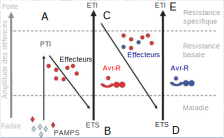
\includegraphics[width=0.8\linewidth]{Evolimunity2}
	\caption[Évolution de l'immunité des plantes d’après le modèle en \og zigzag \fg]{Évolution de l’immunité des 
	 plantes d’après le modèle en \og zigzag \fg, adaptée de \citet{Jones2006}. \\ 
	 A : Les plantes reconnaissent les \glspl{PAMP} (losanges) \textit{via} les
	 récepteurs \glspl{PRR}, ce qui induit la \gls{PTI}. B : Les agents pathogènes sécrètent des facteurs   
	 de virulence (points), qui répriment la \gls{PTI}, permettant la multiplication des agents pathogènes et  
	 conduisant à l’\gls{ETS}. C : Un effecteur  (point rouge) est reconnu spécifiquement par un récepteur (symbole 
	 rouge) codé par un \gls{gene R} de la plante, ce qui active l’\gls{ETI}. D : L’évolution des agents pathogènes  
	 permet l'acquisition de nouveaux effecteurs (en bleu), lui permettant de supprimer l’\gls{ETI} et de déclencher 
	 une nouvelle \gls{ETS}. 
	 E : L’évolution de la plante favorise  de nouveaux \glspl{gene R}, capables de reconnaître les nouveaux 
	 effecteurs, permettant ainsi une nouvelle \gls{ETI}.}
   \label{fig:zigzag}
 \end{figure}
	
      
\subsection{Les résistances qualitatives}
	
	Les résistances qualitatives ou totales sont des résistances monogéniques, reposant sur un \gls{gene R} vis-à-vis d’un agent pathogène. Leur mécanisme d’action  correspond au 
modèle \og gène-pour-gène \fg{}\citep{Flor1971, Moury2010, Thrall2016}.
En 1947, Flor a montré qu'il existe une interaction incompatible entre le lin (\textit{Linum usitatissinum}) et la rouille causée par le champignon\textit{ Melampsora lini}.  Cette relation est basée sur un modèle  gène-pour-gène qui implique qu'un gène d'avirulence (gène \textit{Avr}) chez l’agent pathogène est identifié par un \gls{gene R} chez la plante, entraînant une réaction incompatible, c’est à
dire un blocage de l’agent pathogène par la plante \citep{Dangl2001, Jones2006}; \autoref{tab:GFG}). La reconnaissance très spécifique entre gène \textit{Avr} et \gls{gene R} se produit \textit{via} des récepteurs cytoplasmiques. La résistance qualitative est donc associée à une \gls{ETI}.
Si le \gls{gene R} est inactif ou absent, ou si de manière équivalente le ravageur n'a pas le gène d'\textit{Avr}, l'interaction dite compatible résulte  en une maladie infectieuse. 
	
	
	 \begin{table}[ht]
	    \centering
		  \caption[Modèle d’interaction gène-pour-gène]{Modèle d’interaction gène-pour-gène, 
		           qui stipule qu'un gène 
	     	       avirulent (\textit{Avr}) chez l’agent pathogène est identifié
		           par un gène majeur de résistance  chez la plante.}
		  \label{tab:GFG}
		  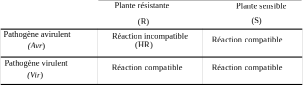
\includegraphics[width=1\linewidth]{GFG2.pdf}  
	 \end{table}
		
	 
	Les \glspl{gene R} sont connus pour de nombreux bioagresseurs  comme des  champignons, oomycètes, virus, bactéries, nématodes et insectes \citep{Dangl2001}. Les  \glspl{gene R}    jouent un rôle important dans le contrôle des maladies 
des céréales comme le blé, le riz et le maïs, mais aussi des cultures maraîchères comme la tomate,
le poivron ou la pomme de terre \citep{Ballvora2002, Hammond-Kosack1997,Schmidt2010, Stuthman2007, Gururani2012, Seid2015,  Pilet2005}.

{\small\medskip \textsc{Remarque --} Le modèle \og matching allele \fg{} est une autre façon de représenter les interactions génétiques entre hôtes et pathogènes. Il suppose que la reconnaissance du pathogène par la plante débouche sur une interaction  compatible, contrairement au modèle gène-pour-gène. L'interaction est généralement fondée sur un seul gène, associé à plusieurs allèles, alors que le modèle gène-pour gène suppose qu'il n'existe que deux allèles (sensible et résistant). Le pathogène peut se développer sur un seul génotype de l'hôte. Dans la version \og inverse matching allele \fg{}, la reconnaissance débouche sur une interaction incompatible, comme le modèle gène-pour-gène, mais toujours pour un seul génotype de l'hôte \citep{Thrall2016}.}


\subsection{Les résistances quantitatives} \label{sec:quantitatives}

	Il existe une autre catégorie  de résistance, les résistances polygéniques  \citep{Cooper1983}. Les traits polygéniques s'expriment sous une forme quantitative  qui peuvent prendre un continuum de valeurs selon les souches
d’agent pathogène, les génotypes de plante et l’environnement \citep{Pariaud2009}.
Les  caractères quantitatifs sont par exemple des caractères mesurables comme le rendement, le taux de succès de l'infection, la période de latence, le taux de croissance. On admet que plusieurs locus ou régions du génome de la plante, portant un ou plusieurs gènes, sont impliqués dans le contrôle de ces caractères et que de nombreux allèles sont responsables de la variabilité. Ces locus sont appelés \gls{QTL}  \citep{Lannou2012}.
On peut noter que lorsque  ces gènes sont associés à la résistance vis-à-vis d’un pathogène, on parle également de \gls{QRL} \citep{Young1996}. Cette résistance polygénique est aussi dite  partielle
ou quantitative,  car elle permet
de ralentir le développement de l’agent pathogène et de baisser l'intensité des symptômes.
Cette résistance est considérée comme  beaucoup plus
fréquente que la résistance qualitative et plus difficile à contourner du fait de son caractère polygénique  \citep{Kearsey1998, Sage-Palloix2007, Parlevliet1989}. 
	
	Bien que   les mécanismes moléculaires sous-jacents à cette résistance polygénique soient encore peu connus, une récente étude a proposé plusieurs mécanismes pouvant contribuer à la mise en place de ce déterminisme polygénique \citep{Poland2009}.
La résistance partielle serait conditionnée par des gènes à effet pléiotrope \footnote{Gène pléiotrope : gène qui détermine plusieurs caractères phénotypiques.}, qui agissent sur la résistance aux pathogènes et sur le
développement des plantes.  
Ceci a été montré pour l'interaction entre \textit{Phytophtora infestans} et pomme de terre, avec la publication de données  sur la colocalisation de \glsplural{QTL} pour la vigueur, la précocité et la
résistance  \citep{Collins1999}.
L’accumulation de composés antimicrobiens au
cours de la \gls{PTI} pourrait ralentir le développement de l’agent pathogène et baisser l’intensité des symptômes. La \gls{PTI} ou la réponse basale serait associée à la résistance  quantitative  \citep{Boller2009}.
Enfin, de nombreux  auteurs considèrent que les facteurs de résistance partielle seraient en réalité  des gènes  majeurs de résistance \og affaiblis \fg{} qui ne permettent pas de stopper complètement le
développement d’un pathogène  \citep{Parlevliet1977, Young1996}. 
Ainsi, \citep{Wang1994} ont  trouvé  des \glsplural{QTL} induisant une résistance partielle dans le pathosystème riz--\textit{Magnaporthe grisea} qui colocalisent avec des \glspl{gene R}. De plus,
lorsqu’un \gls{gene R} a été contourné par une souche de pathogène, ce
gène rendu inefficace permettrait tout de même de réduire le niveau de la maladie. Ce phénomène, appelé  résistance résiduelle  a été rapporté pour plusieurs pathosystèmes \citep{Nass1981, Brodny1986}.

 
\subsection{La  création ou l'amélioration variétale}
 
	L'amélioration variétale classique consiste  à créer de nouvelles variétés à partir de variétés existantes. Elle est apparue avec l'agriculture il y a environ 10\,000 ans.
L'homme cultive alors les plantes  pour son alimentation et pratique une sélection  de manière empirique depuis l'ère néolithique, gardant les graines des plus belles plantes, pour les replanter l'année suivante.
Cela a contribué progressivement à une amélioration de l'espèce cultivée par une sélection  de caractères d'intérêt agronomique  comme la taille des parties consommables (graines, tubercules), les saveurs, la résistance, le rendement. 
L'évolution des techniques de sélection, grâce notamment à la découverte du rôle des organes sexuels chez les végétaux par  Millington-Grew (1676),  des lois  de Gregor Mendel sur la génétique  et l'hérédité \citep{Biffen1905}, des travaux de \citet{Darwin1876}   et de \citep{Shull1908} sur la vigueur des hybrides, ont posé les bases scientifiques de l'amélioration variétale et perpétué cette domestication des plantes. % Au passage, Mendel découvrit ces lois concernant les principes de l'hérédité biologique à partir d'un modèle expérimental sur les petits pois (\textit{Pisum sativum}) en utilisant des procédés d’autofécondations pour produire rapidement un grand nombre de descendants et  %
%À partir des années 1930, l'utilisation de la résistante des plantes   contre
%les bioagresseurs s’est développée de plus en plus \citep{Holmes1938}.  
Les premières variétés hybrides\footnote{Les premières générations d'hybrides (appelé lignées F1) étant hétérozygotes, les semences obtenues à partir de l’autofécondation
de F1 présentent des traits non identiques aux parents. L’utilisation de variétés F1 nécessite donc d’acheter des graines chaque année afin d’hériter des caractères des deux lignées homozygotes pures.} étaient des maïs hybrides, cultivés aux États-Unis à partir des années 1930 \citep{Duvick2001}.
	 
	Aujourd'hui, l'amélioration variétale consiste dans la plupart des  cas  à sélectionner des variétés naturellement résistantes  et de les croiser avec des variétés possédant de bonnes qualités  agronomiques (rendement, vigueur, qualité, valeur nutritive, tolérance aux stress abiotiques) afin de réunir ces caractères dans une seule variété.
Par le choix des meilleures plantes dans la descendance, les sélectionneurs aboutissent après un long travail de sélections successives à la création d'une nouvelle variété, aussi appelée cultivar. Ainsi, les nouveaux cultivars sont tout aussi naturels que les espèces de plantes obtenues par domestication de manière empirique il y a des milliers d'années.  
	
	Lorsqu’un sélectionneur souhaite réaliser l'introgression d'un gène de résistance d'une espèce végétale chez une autre espèce ne possédant pas ce gène, il procède  par croisement  interspécifique
de  deux lignées pures homozygotes  parentales  \citep{Shull1908}, et possédant des caractères d’intérêt qu’il souhaite réunir dans une même lignée. Ce procédé est connu aussi sous le nom d'hybridation. Une fois la lignée \og donneuse \fg{} choisie (ici la lignée résistante), plusieurs rétrocroisements avec la variété cultivée  appelée lignée \og receveuse ou récurrente \fg{} sont  nécessaires pour obtenir une \og  lignée convertie \fg, se rapprochant le plus possible de la variété cultivée mais possédant le gène de résistance.
Cette lignée convertie  sera une lignée pure, stable et reproductible.
L'introgression  du gène \textit{Mi-1} de la tomate vis-à-vis du nématode à galles (genre \textit{Meloidogyne})  en est un exemple typique en culture maraîchère \citep{Milligan1998}. À l'échelle mondiale, c’est le seul gène de résistance actuellement présent dans les variétés de tomate contrôlant plusieurs espèces de nématodes à galles. Ce gène, issu de l’espèce sauvage \textit{Solanum peruvianum}, a été introgressé par croisement interspécifique dans la tomate cultivée \textit{Solanum lycopersicum} et les premières variétés résistantes sont apparues sur le marché à la fin des années 1940 \citep{Smith1944}.
% C’est également de cette manière qu’a été introgressée une résistance chez le blé vis-à-vis du virus \gls{BYDV}  (Sharma et al., 1995).
%Dans le cas du mildiou de la pomme de terre, onze gènes de résistance qualitative identifiés sur l’espèce sauvage \textit{Solanum demissum} ont été  introgressés dans les variétés cultivées \textit{Solanum tuberosum} depuis les années 1950 \citep{Pilet2005, Kuang2005}. 



	L'avancée des connaissances et les progrès technologiques ont permis  la création de nouvelles variétés résistantes, grâce par exemple  au marquage moléculaire et à la transgénèse. %Le marquage  moléculaire  est un marqueur génétique composé de petits fragments d'ADN que l'on appelle amorces ou sondes qui permet de localiser une région particulière du génome de la plante. 
La découverte des marqueurs moléculaires en 1987 et le développement de la PCR (Polymerase Chain Reaction) ont contribué aux premières détections de \glsplural{QTL}. 
La transgénèse correspond, quant à elle, au transfert d'un ou plusieurs gènes provenant d'un cultivar ou d'un autre organisme (bactérie, champignon)  dont l'expression  fait apparaître un caractère  déterminé.  Ces nouvelles variétés sont connues sous le nom d'organismes génétiquement modifiés (OGM). Par exemple,  le maïs \textit{Bt} est une plante transgénique dont la résistance à la pyrale  (un lépidoptère ravageur) est portée par le gène de la bactérie  \textit{Bacillus thuringiensis} (\textit{Bt}) codant la toxine \textit{Cry1Ab}. %  En effet, cette bactérie du sol est mortelle pour la pyrale et  l'innocuité de cette bactérie pour l'homme aurait  été démontrée. %(toutefois des études  continuent à étudier la véracité de cette affirmation).

	%On retrouve comme autre procédé de création variétale, le greffage sur plantes sauvages résistantes. Cette technique semble efficace et particulièrement économique.  Le greffage des légumes est une pratique ancienne. Il a été pratiqué sur certains cucurbitacées  en Chine dès le 1er siècle avant J.C.
%Il s'est vraiment développé à partir de 1920 au Japon avec des porte-greffes courges apportant plus de vigueur aux \textit{Cucurbitacées} telles la pastèque permettant ainsi de diminuer les dégâts. Actuellement, les portes greffes sont  essentiellement utilisés pour les \textit{Solanacées} ($eg.$ tomates et les piments) et les \textit{Cucurbitacées} ($eg.$ melons, concombres, pastèques, courges).

	\begin{figure}[p]
		\centering \includegraphics[width=1\linewidth]{seedvariety.jpg}
		\caption[Perte des variétés ]{Illustration de la perte d’une grande partie 
		         des variétés de fruits et légumes
                 commercialisées entre 1903 à 1983. Source : \citet{NG2011}.}
		\label{loss:varieties}
	\end{figure}

      Au cours du XXème siècle, les sélectionneurs ont créé des nouvelles variétés à partir d'un nombre très limité d'espèce de plantes  d'une culture donnée. 
Cela  a conduit à un appauvrissement important des semences (\autoref{loss:varieties}), de la diversité génétique au sein d'une même espèce  et une plus forte homogénéité dans les paysages agricoles. Par ailleurs, les temps évolutifs entre les agents pathogènes et leurs hôtes sont généralement différent dans les agroécosystèmes. Les agents pathogènes sont généralement à un stade avancé par rapport à leurs hôtes puisqu'ils possèdent un temps de génération plus court et des populations plus importantes, ce qui permet un plus grand nombre de mutations dans une période de temps fixe \citep{Zhan2014}.
Les agroécosystèmes actuels (forte homogénéité des paysages, faible nombres d'espèces de plantes) ont conduit à une évolution uniquement  des agents pathogènes et joue  un rôle majeur dans le contournement des variétés résistantes porteuses de gènes majeurs \citep{Stukenbrock2008}.


\subsection{Contournement et  coût de virulence}
\label{contournement}

	 L'émergence d'agents pathogènes à même de contourner les résistances remet potentiellement en cause l'efficacité de cette méthode de lutte. On parle de contournement de la résistance lorsque tout ou partie de la population d'agents pathogènes s'est adaptée à la résistance et peut dès lors se développer comme s’il s’agissait de plantes sensibles. On parle alors de population \og virulente \fg{} vis-à-vis du gène de résistance concerné \footnote{En biologie évolutive, la virulence est assimilée à la mort de l'hôte due à l'infection. Par souci de clarté dans ce manuscrit, quand on parle de ce type de virulence, on utilise le terme agressivité.} \citep{McDonald2002}. Les \glspl{gene R} sont rares et la plupart des sélectionneurs se concentrent sur l'introgression des principaux \glspl{gene R} dans les variétés végétales \citep{Zhan2015}. Par conséquent, les agriculteurs cultivent finalement la même résistance sur plusieurs années et à grande échelle en monoculture.  Par exemple, en 1969, 85~\% du maïs produit aux États-Unis était de la même variété.
  En 1970, les épidémies  d'helminthosporiose du maïs  (Southern Corn Leaf Blight) et de la \og brûlure jaune des feuilles du maïs \fg{} (Yellow Leaf Blight of Maize) dues respectivement aux champignons \textit{Cochliobolus heterostrophus} (race T) et  \textit{Mycosphaerella zeae-maydis}    ont détruit 17~\% de toutes les cultures de maïs aux États-Unis \citep{Pring1989}.

	 L'introduction de cultivars résistants  provoque un changement des pressions de sélection sur le bioagresseur.  Si un pathogène avirulent perd le gène d'\textit{Avr} à la suite de mutations ou recombinaisons aléatoires, cela peut conduire   à l'émergence et à l'établissement d'un variant pathogène virulent  \citep{McDonald2002, Castagnone-Sereno2002, Garcia-arenal2003a, Parlevliet2002, Moffat2001}. Par la suite, le variant virulent possédant un avantage sélectif par rapport au pathogène avirulent  sur le cultivar résistant, il peut éventuellement s'établir dans la population globale.  En quelques années ou en quelques mois, le bénéfice
fourni par les cultivars résistants peut être annulé en raison de la capacité du pathogène virulent à se propager et à se reproduire \citep{McDonald2002, Parlevliet2002}. Par conséquent, l'agriculture moderne, de par son absence ou manque de diversité génétique chez l'hôte, est  particulièrement exposée aux contournements de résistances et à l’émergence de
nouveaux agents pathogènes \citep{Stukenbrock2008, Anderson2004}. L’identification et l'utilisation accrue de nouveaux cultivars résistants par  les agriculteurs conduit inévitablement à un cycle qui épuise le stock des résistances naturelles des plantes. Ce cycle continu commence par la création d'une nouvelle variété, qui est ensuite déployée jusqu'à une perte quasiment totale de l'efficacité des \glspl{gene R}. Elle est alors remplacée par une nouvelle variété résistante et le cycle recommence... Ce cycle est connu sous le nom de \og boom and bust \fg{} (expansion-récession) \citep{Brown2011, Brown2015, Zhan2015}.

	Pour de nombreux pathosystèmes, l’introduction d’une variété résistante dans un paysage
agricole  conduit souvent à  un  contournement rapide de la résistance par les agents pathogènes. À titre d’exemple, grâce notamment aux travaux de \citet{Moury2010}, le contournement d’une résistance par un virus est un processus bien décrit, qui peut se généraliser à de nombreux pathogènes. Il existe trois étapes
dans le contournement d’une résistance.  La première étape consiste en l’apparition d’un
variant virulent, dans une population avirulente, par une ou plusieurs mutations ou recombinaisons dans un gène d’avirulence (voir Encadrés~\hypertarget{mut2}{\hyperlink{mut1}{La mutation}} et \hypertarget{recomb2}{\hyperlink{recomb1}{La recombinaison}}). 
 Deuxièmement, il faut assurer le maintien de ces mutations
dans la population. Les variants virulents et avirulents sont en compétition et l'issue de cette compétition en faveur des virulents dépend de l’avantage sélectif que ce nouveau caractère leur
procure et de la disponibilité des hôtes compatibles. La fitness de chaque variant, c’est à dire la capacité d’un individu à survivre et à se reproduire, ou encore la capacité d’un individu à transmettre ses gènes à la génération suivante, est un facteur clé pour le maintien et la multiplication des variants virulents. La sélection
des individus les mieux adaptés et la dérive génétique sont deux forces évolutives qui vont
conditionner le maintien d’une population virulente dans un environnement donné \citep{McDonald2002a} (voir Encadrés~\hypertarget{selec2}{\hyperlink{selec1}{La sélection}} et \hypertarget{der2}{\hyperlink{der1}{La dérive}}). La troisième étape se réfère à la capacité de migration du pathogène qui, associée à la sélection et la dérive génétique, permet la fixation du variant dans la population \citep{Brown2002, Charlesworth2009} (voir Encadré~\hypertarget{mig2}{\hyperlink{mig1}{La migration}}).

	Dans la littérature, de nombreux exemples de contournement de résistance ont été signalés.
Par exemple, chez  le phoma du colza (\textit{Leptosphaeria maculans}),  le contournement des résistances \textit{Rlm1}, \textit{Rlm2}, \textit{Rlm4} et \textit{Rlm9} a été démontré après trois ans de culture \citep{Rouxel2005, Rouxel2003}.
Dans le cas du mildiou de la pomme de terre (\textit{P.~infestans}), le contournement des  gènes majeurs de résistance  a été démontré après 5 à 7 ans de culture  \citep{Pilet2005, Kuang2005, Montarry2006}. 
En cultures maraîchères, l’exemple le plus typique est celui du contournement du gène \textit{Mi-1} de la tomate par des nématodes à galles des racines \citep{Castagnone-Sereno2002}. 


\subsubsection*{Coût de virulence}

	La virulence chez la plupart des pathosystèmes est généralement associée à un coût de virulence, appelé également coût de fitness, sur les plantes sensibles et résistantes, qui se traduit souvent par une diminution de la fertilité et/ou de la fécondité \citep{Laine2013, Brown2003} (\autoref{tab:cout}). 
De nombreuses études ont fait état de ce coût de fitness chez des bactéries \citep{Cruz2000, Leach2001}, des oomycètes \citep{Montarry2010}, des virus \citep{Garcia-Arenal2013}
 ou des nématodes \citep{Castagnone-Sereno2002, Castagnone-Sereno2007, Djian-Caporalino2011}. L'existence de coûts de fitness implique que même si les variants virulents sont
sélectionnés sur les cultures résistantes, ils sont  contre-sélectionnés sur les cultures sensibles, où les avirulents  se développent et se reproduisent plus rapidement.

 \begin{table}[ht]
  \centering
   \caption[Interactions entre hôte sensible ou résistant et pathogène avirulent ou virulent, d'après    
          \citet{Leonard1977, Leach2001}]{Interactions entre hôte sensible (susceptible) ou résistant et pathogène  
          avirulent ou virulent, d'après \citet{Leonard1977, Leach2001}. Le succès de l'infection, compris entre 0 (pas 
          d'infection) et 1 (efficacité maximale), peut être réduit par le coût de virulence ($k\in[0,1]$) et 
          l'efficacité de la résistance ($c\in[0,1]$), avec $c=1$ pour une résistance totale/qualitative.}
   \label{tab:cout}
		  \begin{tabular}{c}
		  \includegraphics[width=0.8\linewidth]{Leach.pdf}
		  \end{tabular}
 \end{table}

	L’analyse  des compromis évolutifs pour les modèles gène-pour-gène ont été étudiés par de nombreux auteurs  \citep{Leonard1977, Tellier2007, Brown2015}. Un compromis évolutif peut se définir par  le  choix auquel est contraint un parasite afin de maximiser sa  valeur sélective dans un contexte dans lequel les ressources sont limitées. 
Dans le cas des agroécosystèmes naturels, la coexistence de génotypes de parasites avirulents et virulents en présence d'hôtes sensibles et résistant, résulte d'un compromis évolutif. Ce polymorphisme est dû à des coûts  de virulence qui empêcheraient tout génotype virulent de se diriger vers la fixation \citep{Laine2013}. 


%	\begin{figure}
%		\centering \includegraphics[width=0.7\linewidth]{brown.pdf}
%		\caption{ Illustration de la co-évolution hôte-parasite  impliquant un  simple modèle gène-pour-gène. Source :   \citep{Brown2015} 
%		}
%		\label{co:evolution}
%	\end{figure}

\hypertarget{mut1}{}
\begin{encadre2}{La mutation}
\hyperlink{mut2}{$\curvearrowleft$}
	La mutation correspond à des modifications dans  la séquence
nucléotidique dans le génome d'un individu. Cette force évolutive est la principale source de variation génétique. C’est le mécanisme majeur
d’apparition des virulences, en particulier chez les bactéries et les virus, dont la taille conséquente des populations entraîne  plus grand nombre de mutations \citep{McDonald2002}. Parmi les agents pathogènes des plantes, le taux
de mutation des eucaryotes est compris entre $10^{-9}$ et $10^{-11}$, tandis que chez les bactéries il est
estimé à $10^{-9}$. Les virus montrent des taux de mutation entre $10^{-4}$ et $10^{-8}$ \citep{Drake1998,
Drake1999}. Pour davantage d'exemples, voir \citep{Lynch2010}. 
%Il existe trois types de mutations dites ponctuelles : les mutations par substitution correspondant au changement d’un seul nucléotide,  les mutations par insertion et les mutations par délétion.
\par
Chez les champignons et les bactéries, l’acquisition de
virulences résulte souvent de la délétion ou de l'insertion
d’un fragment d’ADN, qui a pour conséquence l’inactivation du gène d’avirulence
\citep{Kang2001, Gout2007}.
Par exemple, la virulence de certaines souches du champignon \textit{Leptospheria maculans} vis-à-vis du gène de résistance \textit{Rlm1} du colza (\textit{Brassica napus}) est due à une délétion dans le gène d’avirulence \citep{Gout2007}. Chez les virus, l’acquisition de virulence se fait
essentiellement \textit{via} des mutations par substitution nucléotidique et souvent un très
faible nombre de mutations est suffisant pour le contournement de la résistance  \citep{Jenner2000, Moury2004, Janzac2010}. 
Chez les nématodes à galles, l'émergence d'un variant virulent  pourrait être provoquée par des facteurs génétiques et/ou épigénétiques. 
Dans le cas des nématodes à galles (\textit{Meloidogyne}),  des mutations par substitution nucléotidique (ou variations nucléotidiques) ont été trouvées entre
nématodes avirulents et virulents lors d' études expérimentales
\citep{Neveu2003, Semblat2001}. Cependant, très peu de choses sont connues sur les  différents   mécanismes sous-jacents \citep{Castagnone-Sereno1994, Castagnone-sereno2019}.
\end{encadre2}

\hypertarget{recomb1}{}
\begin{encadre2}{La recombinaison}
  \hyperlink{recomb2}{$\curvearrowleft$}
     La recombinaison correspond à un échange d’information génétique entre deux
génomes différents. En fonction du type d'organismes, la
recombinaison se produit de différentes façons :  lors de la reproduction sexuée chez
les eucaryotes, lors de conjugaison bactérienne chez les procaryotes, ou lorsque
plusieurs  virus infectent simultanément une même cellule.
\par
Lorsque  plusieurs allèles de virulence sont nécessaires au contournement d’une résistance (\textit{e.g.} contournement d'un gène pyramidé), la recombinaison accentue les phénomènes de contournement par rapport  à la mutation, car cette dernière nécessite plusieurs événements successifs \citep{McDonald2002}.
\end{encadre2}


\hypertarget{selec1}{}
\begin{encadre2}{La sélection}
  \hyperlink{selec2}{$\curvearrowleft$}
	La sélection fait varier les fréquences alléliques dans les populations et permet de favoriser  les génotypes les mieux  adaptés aux conditions locales. C'est un mécanisme évolutif moteur dans l'évolution des espèces qui permet d'expliquer l'adaptation d'un individu dans un milieu donné \citep{Darwin1859}.
Ce processus évolutif entraîne l’augmentation  ou la diminution  de la fréquence de certains génotypes  en fonction de leur effet sur la reproduction ou la survie des individus (valeur sélective).
% La sélection est la principale force qui détermine les changements de fréquence des allèles mutant \citep{McDonald2002}.
	
	La sélection peut être de trois types : stabilisante, diversifiante ou directionnelle.
La sélection stabilisante permet de favoriser  la fixation des phénotypes moyens par rapport
aux phénotypes extrêmes. On retrouve ce type de sélection au niveau du poids des mammifères à la naissance,
pour lequel deux sélections s’opposent: un poids élevé augmente les chances de
survie  de l'enfant (meilleur accès aux ressources, meilleure défense) mais baisse la
probabilité de survie de la mère, alors qu’un poids faible favorise la survie de la
mère mais diminue la probabilité de survie de l’enfant \citep{Covas2002}.
La sélection diversifiante tend à favoriser la fixation des phénotypes extrêmes par
rapport aux phénotypes moyens. Ce type de sélection a pour conséquence d'éliminer les phénotypes intermédiaires.%L'exemple le plus connu est la taille des becs des pinsons ponceau à ventre
%brun (\textit{Pirenestre ostrinus}). Ces oiseaux 
%peuvent se nourrir de grosses graines ou  de petites en fonction de leur milieu. Seuls les oiseaux possédant un
%gros bec peuvent casser les coquilles dures des grosses graines tandis que les 
%oiseaux à petit bec sont assez adroits pour se saisir des petites. Les oiseaux avec
%un bec intermédiaire possède un désavantage sélectif car ils ne sont pas capables d’ouvrir les
%grosses graines et sont moins habiles  pour se saisir des petites (Smith, 1993). 
La sélection directionnelle tend à favoriser
des  traits phénotypiques (ou génotypiques) d'un extrême par rapport aux autres.
Ce type de sélection est souvent rencontré lorsqu’une population subit  des changements environnementaux abrupts.

	Depuis des  millénaires, les agents pathogènes et les plantes se sont engagés dans une bataille évolutive, les agents pathogènes tentant de surmonter les défenses des plantes et les plantes tentant de résister aux attaques des agents pathogènes \citep{Zhan2015}. 
Dans les écosystèmes naturels, ces processus co-évolutifs
ont permis de retarder et/ou diminuer les épidémies grâce à une hétérogénéité spatiale et/ou temporelle de l’environnement  \citep{Zhan2015, Burdon2014}. 
L’introduction à grande échelle d’un cultivar portant un gène de résistance à un agent pathogène   induit une pression de sélection directionnelle sur l'agent pathogène ciblé. 
La monoculture peut être ainsi considérée comme une pression de sélection directionnelle en faveur des individus virulents capables d’infecter les plantes porteuses du gène de résistance.% En effet,
L'utilisation de pesticides chimiques peut conduire également à une sélection directionnelle \citep{Pimentel1985}.
\end{encadre2}

\hypertarget{der1}{}
\begin{encadre2}{La dérive génétique}
  \hyperlink{der2}{$\curvearrowleft$}
La dérive génétique correspond à des fluctuations aléatoires de la fréquence des génotypes au sein d’une même population \citep{Henry1999}. 
La dérive génétique a comme conséquence la perte d’allèles et donc la  réduction de la variabilité génétique. La dérive génétique influence les dynamiques évolutives indépendamment des génotypes présents dans la population, car elle repose sur un processus aléatoire (contrairement à la \hyperlink{selec1}{sélection}).
\par
Il est important d’introduire le concept de taille efficace d’une population pour illustrer les conséquences de la dérive génétique. La taille efficace correspond au nombre d’individus au sein d’une population  transmettant de manière \og efficace \fg{} leurs gènes à leurs descendants.  Ainsi, la taille efficace d’une population peut être définie comme la taille d'une population \og idéale\fg{} présentant les mêmes fluctuations de fréquences d'allèles que la population étudiée  \citep{Gutierrez2012}.
La taille efficace est généralement plus petite que la taille réelle de la population \citep{Charlesworth2009}. 
 Plus la taille efficace est petite, plus l’effet de la dérive est élevé et donc plus la perte de  variabilité génétique est grande \citep{McDonald2002}. En particulier, pour des populations  soumises à la dérive génétique (notamment chez les virus), une petite taille efficace peut mener à la perte de mutations associées à la virulence et ainsi éviter ou réduire les risques  de contournement d'une résistance, augmentant ainsi sa durabilité \citep{Rousseau2019}.
\end{encadre2}

\hypertarget{mig1}{}
	\begin{encadre2}{La migration}
\hyperlink{mig2}{$\curvearrowleft$}
      La migration  est un processus par lequel des allèles (gènes) ou des individus (génotypes) particuliers sont échangés entre des populations géographiquement séparées \citep{McDonald2002}.
Dans un système de populations interconnectées, les nouvelles
mutations conférant un avantage adaptatif peuvent ainsi se propager entre les populations \citep{Burdon1999}.
\par
Ce phénomène peut entraîner l’arrivée de pathogènes virulents dans une culture où ils sont initialement absents, à cause de la présence de variants à proximité de la culture  (\textit{e.g.} plantes sauvages). L'homme peut aussi être à l'origine de la migration d'agents pathogènes, à cause de pratiques culturales par exemple  \citep{Brown2002, Burdon1993}. Ainsi, la dispersion d'agents pathogènes peut être possible au-delà des capacités naturelles de dispersion de ces derniers.  
\end{encadre2}


\section{Durabilité des résistances} \label{durabilite}
    
\subsection{Définitions}
	
	\citet{Johnson1984} a défini qu’une résistance était durable lorsqu’elle restait efficace suite à son déploiement sur une longue durée et à grande échelle, dans un environnement favorable au développement
du pathogène. %Ainsi, on peut quantifier la durabilité d’une résistance après un
%déploiement de la résistance sur un horizon temporel long et dans la plupart du temps une fois
%que la résistance ai été contournée  \citep{Johnson1981}. 
%La durabilité d’une résistance est donc fortement corrélée avec le contournement de la résistance.
%La durabilité va donc principalement dépendre du temps nécessaire pour l'acquisition d'une ou plusieurs  mutations chez l'agent pathogène et de la capacité des agents pathogènes virulents à s'établir dans la population (mode de reproduction, mode de dispersion, taille des populations) (Barrett et al,
%2008 ; Brown, 2015 ; Macdonald2002,  Stuthman et al, 2007 ; van den Bosch et al, 2007.
%Gilligan, 2003 ; Zhan et al, 2015).
La durabilité d’une résistance diffère  en fonction des systèmes hôtes-pathogènes. Plus une résistance est difficilement contournable, plus elle est durable.
La résistance qualitative aux maladies des plantes est connue pour avoir une faible durabilité vis-à-vis des pathogènes fongiques, bactériens et viraux \citep{Garcia-Arenal2003, Brown2015, Parlevliet2002}. Néanmoins, il existe des gènes de résistance qualitative durable comme le gène \textit{Tm2} chez la tomate et le gène \textit{N} chez le tabac contre le tobacco mosaic virus pour lesquels on n'a pas observé de contournement   \citep{Parlevliet2002}.
Par ailleurs, il a été démontré qu'une résistance quantitative serait plus durable qu'une résistance qualitative \citep{Mundt2014, Palloix2009}. Par exemple, la résistance à la rouille des feuilles de l'orge (\textit{Puccinia hordei}) observée chez les cultivars d'orge Minerva et Vada est une résistance  polygénique qui est aussi efficace aujourd'hui que lors de sa première utilisation en \textit{1955} \citep{Parlevliet2002}. 
Pour les nématodes (du genre \textit{Meloidogyne}), le
gène de résistance \textit{Mi-1} commercialisé depuis 60 ans, procure une durabilité assez stable \citep{Williamson2006}, bien que des contournements aient été observés ces dernières décennies à l'échelle mondiale  \citep{Castagnone-Sereno2002, Verdejo-Lucas2009,Seid2015}. 

	La définition de la durabilité par \citet{Johnson1984} est qualitative \footnote{La définition de la durabilité par \citet{Johnson1984} ne permet pas de mesurer la durabilité d'une résistance de manière quantitative et ainsi de comparer les durabilités.}. 
Il existe également des métriques quantitatives de durabilité, en lien avec des critères comme la fréquence d'agents pathogènes virulents ou encore le rendement. On retrouve dans la littérature des approches expérimentales pour mesurer la durabilité.
\citet{Barbary2014}, par exemple, ont étudié la durabilité des \glspl{gene R} \textit{Me1}  et \textit{Me3}  aux nématodes \textit{Meloidogyne incognita} en inoculant des nématodes avrirulents à très forte concentration puis en calculant le pourcentage de plantes présentant plus de 5 galles. Ce seuil permet de déterminer si la résistance a été contournée ou non. 
Cependant, dans un modèle \og gène-pour-gène  \fg, la durabilité d'une résistance dépend du temps nécessaire pour l'acquisition d'une ou plusieurs  mutations chez l'agent pathogène et de la capacité des agents pathogènes virulents à s'établir dans la population hôte sur des échelles spatiales plus ou moins larges \citep{Barrett2008, Brown2015, McDonald2002,  Stuthman2007, vandenBosch2003, Zhan2015}. Cette capacité dépend en particulier du niveau d’agrégation spatiale et/ou temporelle des variétés hôtes, ainsi que de la structure et la dynamique démo-génétique de la population de pathogènes (qui dépend du mode  et du taux de reproduction, de la dispersion, de la taille des populations, des coûts de fitness, \textit{etc.}). La prise en compte des facteurs épidémiologiques, démographiques, génétiques  et de leurs interactions  est donc importante pour quantifier la durabilité d'une résistance. Ceci est difficilement réalisable par des approches expérimentales à cause du temps et du coût de la mise en place d'expériences de terrain à grande échelle.

	Les approches de modélisation mathématique permettent d'évaluer et/ou de comparer l'efficacité et la durabilité des résistances, sur des échelles de temps longues et des échelles spatiales allant de la plante au paysage agricole. \citet{vandenBosch2003} ont proposé, à partir d’un modèle mathématique, trois mesures quantitatives de la durabilité : (i) le nombre d’hôtes non infectés  jusqu’à ce que  la résistance soit contournée,
c’est à dire que la fréquence de virulents ait dépassé un certain seuil ; (ii) le temps écoulé entre
l’introduction du cultivar résistant et le moment où la fréquence de pathogènes virulents, présents initialement, atteint un seuil prédéfini, par exemple 90~\% ; (iii) le délai d’invasion, c’est-à-dire la durée nécessaire au  pathogène virulent pour envahir les cultures de plantes résistantes, sachant qu’il est absent
de la parcelle avant l’introduction de la résistance. 
La plupart des modèles de la littérature utilisent la définition (ii) \citep{vandenBosch2003, Fabre2015, Lof2017}.

%La fréquence seuil de virulents au-delà de laquelle la résistance est considérée comme contournée est clairement arbitraire et dépend de facteurs socio-économiques \citep{Bourguet2016}.

	Dans le \autoref{article}, nous avons défini la durabilité comme le nombre de saisons au bout duquel une stratégie de déploiement composée uniquement de plantes résistantes engendre une perte de rendement relative par rapport au temps initial (\textit{i.e.} la première année de culture) supérieure à un seuil prédéfini, par exemple 1~\%. Cette mesure de durabilité est fondée sur le rendement des cultures et non la fréquence des virulents, comme dans les trois mesures proposées. 	
		
% Cette thèse a comme but la recherche  de stratégies optimales de déploiement des résistances en utilisant des principes éco-évolutifs afin d'améliorer leur efficacité et leur durabilité. Ces principes permettent de retarder l'évolution des pathogènes et d'augmenter significativement les rendements des cultures, sans l'utilisation des pesticides chimiques. L'identification de ces stratégies pourra permettre de mieux gérer le déploiement des résistances dans les agroécosystèmes et  une meilleur protection des résistances naturelles des plantes.
	 Nous allons exposer dans la suite  comment augmenter la durabilité des résistances
et le rendement des cultures à long terme grâce à des stratégies basées sur des principes
éco-évolutifs qui permettent de retarder l’émergence et/ou l’établissement des populations
virulentes  \citep{Zhan2015, Zhan2014, Brown2015, Bourguet2016}.
	 
    
\subsection[Comment améliorer la durabilité et l'efficacité des résistances variétales ?]{Comment améliorer la durabilité et l'efficacité des résistances des plantes dans les agroécosystèmes ?}
\label{durabilite_sub}

	Favoriser l'hétérogénéité spatiale et/ou temporelle des pressions de sélection dans les agroécosystèmes est la méthode la plus prometteuse afin de gérer durablement le déploiement de la résistance des plantes \citep{Zhan2015, Brown2015, Bourguet2016}. Ces stratégies sont similaires  à celles utilisées pour retarder l'évolution de la résistance aux médicaments et aux pesticides \citep{Bourguet2016, Consortium2013}.
On peut citer principalement quatre stratégies  :
(1) la combinaison de
plusieurs gènes de résistance dans la même plante (pyramidage) ; (2) l'utilisation de 
différents cultivars au sein d'un même champ (mélanges) ou  (3) entre les champs (mosaïques) ;
(4) l'alternance dans le temps de cultivars différents (rotation).
De nombreuses études expérimentales et de modélisation ont démontré l'effet bénéfique de ces stratégies pour augmenter le  rendement des cultures  et la durabilité des résistances \citep{Fabre2012,  Djian-Caporalino2014, Mundt2014, Fabre2015, Bourguet2016}. En outre, de rares études expérimentales  \citep{Djian-Caporalino2014} et différents travaux de modélisation \citep{Bourguet2016, Lof2017, Rimbaud2018} ont comparé la durabilité de ces stratégies. Sur la base des résultats  menées sur la gestion des résistances aux pesticides et aux médicaments \citep{Consortium2013}, \citet{Bourguet2016} hiérarchisent les stratégies en termes de durabilité des résistances aux maladies comme suit : 
pyramidage $>$ mélanges de variétés et mosaïques  $=$ rotation $>$ usage d'une résistance qualitative en monoculture. Toutefois, de nombreuses études ont démontré qu'il n'existe pas de stratégie universellement meilleure que les autres en termes de durabilité \citep{Rimbaud2018, Fabre2012, Djidjou-Demasse2017}. Par exemple, \citet{Sapoukhina2009}, par une approche de modélisation du déploiement spatial des gènes de résistance, a constaté que le pyramidage était tout aussi efficace qu'un mélange aléatoire de cultivars résistants monogéniques. Nous allons voir dans la suite et de manière plus détaillé, les différentes stratégies pour le contrôle des agents pathogènes et pour augmenter la durabilité des résistances des plantes. 
 
\subsubsection{Le pyramidage} \label{sec:durabilite_pyramidage}

	La stratégie la plus courante  consiste à pyramider plusieurs gènes de résistance majeurs en un seul cultivar, dans l'espoir que l'agent pathogène ne puisse pas facilement acquérir la séquence de mutations lui permettant de contourner les différents  gènes de résistance \citep{McDonald2002}.  
Dans sa revue, \citet{Mundt2018} retrace plus en détails le succès du pyramidage.
Le dogme standard a été que, si les gènes de résistance n'ont pas encore été déployés individuellement, la probabilité qu'un agent pathogène asexué acquière le facteur de  virulence contre tous les gènes de résistance pyramidés est très faible  \citep{Schafer1985}.
L'efficacité du pyramidage de \glspl{gene R} repose sur plusieurs hypothèses clés, sans lesquelles elle pourrait être compromise  : (1)
les mutations pour l'acquisition de la virulence sont indépendantes, (2) les virulences ne sont pas préexistantes dans la population de l'agent pathogène, (3) la résistance conférée par chaque gène pyramidé n'a pas encore été contournée, (4) les gènes de résistance  ont  des modes d'action non redondants \citep{Bourguet2016}.
%Il a été démontré que les gènes d'avirulence agissent également comme effecteurs de la virulence et qu'il existe une redondance considérable entre les effecteurs \citep{Jones2006, Cunnac2011}. 
 Par ailleurs, \citet{Leach2001} soutiennent  qu'il existe une relation de cause à effet entre le coût de fitness associé à la virulence  et la durabilité des \glspl{gene R} correspondants.
Ils ont donc émis l'hypothèse que, le pyramidage de gènes ayant un coût de fitness élevé, il devrait être durable.
 Il est attendu que la recombinaison dans le génome d'un agent pathogène soit un mécanisme susceptible de désavantager cette stratégie \citep{Burdon2014, Mundt2014, Brown2015}, car l'agent pathogène pourrait combiner par la suite des mutations présentes dans différents variants du pathogène pour contourner la résistance.

	
	\citet{Rimbaud2018} ont utilisé un modèle mathématique stochastique afin d'évaluer la durabilité du pyramidage de deux \glspl{gene R} pour le contrôle d'une maladie fongique.
Ils ont montré que le pyramidage  est très durable et efficace, car contourner cette résistance totale nécessiterait l'acquisition simultanée de virulences aux deux \glspl{gene R} à forts coûts de fitness.
%Cette stratégie permet de diminuer les risques de contournement et d'augmenter la durabilité des résistances par rapport au déploiement d'un seul gène de résistance \citep{Vu2014, Mundt2018, Pink2002}. 
\citet{Rimbaud2018a}, dans une nouvelle étude, ont comparé les quatre  principales stratégies de déploiement de la résistance des céréales à la rouille (\textit{Puccinia}). Ils ont montré que le pyramidage de gènes était moins  susceptible d'être contourné, mais que les conséquences pourraient être  désastreuses si cela se produisait. En effet, à long terme la forte pression de sélection directionnelle induit une adaptation de l'agent pathogène sur l’ensemble des résistances qualitatives pyramidées; cela conduit à l'émergence d'un variant double-virulent  et  à une perte de l'efficacité des résistances qualitatives (notamment en absence de coût de fitness \citep{Lof2017}). Par exemple, deux gènes de résistance qualitative  pyramidés de  la tomate vis-à-vis du champignon \textit{Cladosporium fulvum} ont été  simultanément contournés suite à l’apparition de pathogènes double-virulents, rendant inefficace toutes les résistances qualitatives \citep{Lindhout2002}.
	
	Des études ont démontré que la combinaison des résistances quantitatives avec une résistance qualitative fournit une meilleure protection des gènes majeurs de résistance \citep{Palloix2009, Brun2010, Delourme2014}. Ces études testent l'efficacité et/ou la durabilité de cultivars résistants impliquant l'introgression d'un \gls{gene R} dans des fonds génétiques \og résistants \fg{} (résistance quantitative). Ainsi,  \citet{Palloix2009} ont  démontré pour  l'interaction piment (\textit{Capsicum annuum}) –  \gls{PVY} que la durabilité du gène de résistance  \textit{pvr2}$^3$  dépendait du fond génétique de la plante dans lequel il était introgressé. \citet{Quenouille2014}, par une étude expérimentale  ont ensuite démontré que l'amélioration de la durabilité correspondait à des \glspl{QTL} de résistance présents dans le fond génétique. Cet effet pourrait résulter d'une réduction de la probabilité de fixation des mutations  bénéfiques pour le virus. Autre exemple, le pyramidage d’un gène de
résistance qualitative \textit{Rlm6}  avec des résistances partielles a montré une durabilité plus intéressante par rapport à une résistance qualitative seule chez le colza \textit{Brassica
napus}  vis-à-vis du champignon \textit{Leptosphaeria maculans} \citep{Brun2010}.
Pour les nématodes à galles, la résistance partielle du piment vis-à-vis des nématodes à galles permet également d'améliorer 
la durabilité ainsi que l'efficacité des \glspl{gene R}  \citep{Barbary2014}.
Cette  plus forte durabilité s'explique  vraisemblablement  par le fait que la résistance quantitative est polygénique, alors que la résistance qualitative dépend d'un seul gène de résistance majeur \citep{Mundt2014, Parlevliet1989}. La résistance polygénique permet de relâcher la  sélection qui s'opère sur les agents pathogènes virulents, contrairement à une résistance qualitative où la sélection est unidirectionnelle \citep{Quenouille2014, Bourguet2016}.

	Dans une autre étude de modélisation, \citet{Rousseau2019} ont étudié l’effet de stratégies de mélanges variétaux dans le but d’augmenter la durabilité des résistances aux virus. Le paysage agricole qu’ils ont étudié comprenait  deux variétés de plantes en mélange, une sensible et une résistante, et deux variants pathogènes, un avirulent et un virulent. 
Dans cette étude, ils ont testé  si la combinaison d'une résistance quantitative réduisant le goulot d'étranglement de la population virale (diminution du $Ne$) avec une résistance qualitative peut augmenter la durabilité de cette dernière. 
Ils ont comparé  les rendements d'un mélange de cultivars sensibles et résistants combinant une résistance qualitative avec une résistance quantitative (pyramidage) et d'un autre comprenant des cultivars sensibles et résistants portant une résistance qualitative (résistance monogénique).
Ils ont montré que les rendements d'un mélange avec la variété pyramidée étaient plus notables  qu'un mélange avec la variété résistante portant un \gls{gene R} pour des coûts de fitness intermédiaires. La stratégie optimale impliquant la résistance pyramidée pourrait fournir jusqu'à 95 \%  de rendement supplémentaire par rapport à un mélange impliquant la résistance qualitative seule.% En effet,
%pour les coûts de fitness élevés, la résistance était durable si bien que le rendement de la stratégie optimale
%ne pouvait être que marginalement augmenté. À l’inverse, pour les faibles coûts de fitness la résistance était
%inefficace et n’apportait aucun bénéfice dans la stratégie optimale. Pour des coûts de fitness intermédiaire, la résistance quantitative contrôlant la taille des goulots d'étranglement peut protéger une résistance qualitative en diminuant la probabilité de succès de la transmission de l'infection des plantes sensibles infectées aux plantes résistantes saines (voir encadré  \hyperlink{der1}{\hypertarget{der2}{La dérive}}) }.

	En conclusion, l'efficacité de cette stratégie seule repose sur le fait que l'acquisition de plusieurs virulences  est très difficile et qu'elle est très probablement associée à de forts coûts de fitness \citep{Brown2015, Leach2001, Fabre2009, Janzac2009}. 


\subsubsection{Les mélanges et mosaïques}
\label{subsubsec:mel}

	L'hétérogénéité des hôtes peut être assurée par  mélanges de différents cultivars  au sein d'une même parcelle  ou entre les parcelles (mosaïques de cultivars) \citep{Keesing2006, Mccallum2015}. Ces stratégies  permettent  de limiter les risques de contournement des résistances des plantes en jouant sur les pressions sélectives. L'idée standard qui contribue au  succès de cette stratégie est qu'elle perturbe la sélection directionnelle, en favorisant différents allèles ou génotypes virulents à différents endroits, retardant par conséquent la montée en fréquence de l'allèle ou du génotype virulent \citep{McDonald2002}. 
Les mélanges et les mosaïques de cultivars contribuent ainsi à améliorer le contrôle épidémiologique et la durabilité des résistances \citep{Burdon2016, Burdon2014}.
	
	Différents modèles théoriques et expériences ont pu démontrer l’effet bénéfique des mélanges de cultivars hôtes en termes de contrôle épidémiologique \citep{Zhu2000,  Mundt2002, Wolfe1985, Kiyosawa1982, Garrett1999}.
Dans sa revue,  \citep{Mundt2002} détaille notamment plusieurs facteurs influençant l'effet des mélanges pour le contrôle des maladies dans un paysage agricole.
Premièrement, on s'attend à ce que l'efficacité des mélanges diminue avec la proportion d’autoinfections\footnote{L'autoinfection  signifie que le parasite est né dans l'hôte qu'il infecte, alors que l'alloinfection signifie que le parasite est arrivé d'ailleurs et qu'il a donc dû se déplacer vers son hôte. La première infection de tout individu hôte sain doit être une alloinfection.}, qui est influencée à la fois par les caractéristiques de l'agent pathogène et de l'hôte.
Deuxièmement, des modèles mathématiques ont montré que l'efficacité des mélanges décroissait
avec la capacité de dispersion de l’agent pathogène \citep{Fitt1986}. 
Troisièmement, des expériences en conditions contrôlées et des études numériques ont montré que l'efficacité des mélanges était moindre pour les parasites générant de grandes lésions, à cause d'une saturation des  plantes infectées \citep{Lannou1994}. 

 %Au delà  de ces facteurs assez généraux, nous verrons dans la suite que  lorsque l'on considère  une stratégie de mélange ou de mosaïque entre cultivars sensibles et résistants, d'autres  facteurs comme le ratio de plantes résistantes, l'hétérogénéité spatiale des hôtes  jouent un rôle très important dans le succès de la stratégie. 
	
	Dans les agroécosystèmes,  le but des mélanges variétaux peut être  de protéger les cultivars sensibles, en les combinant avec des cultivars résistants. En effet, les variants avirulents ne peuvent pas se développer sur  les plantes résistantes et l'existence de coûts de fitness implique que les virulents sont contre-sélectionnés sur les cultures sensibles. Le mélange des deux cultivars permet de combiner ces deux effets et ainsi de contrôler les variants avirulents et virulents.
Cette relation entre la diversité des hôtes et la transmission de la maladie s'explique principalement par un effet de dilution \citep{Mundt2002}.   L'augmentation de la diversité génétique des cultures devrait réduire le taux de transmission des agents pathogènes et diminuer l'intensité des épidémies \citep{Mundt2002}.
Plusieurs approches visant à améliorer la durabilité des \glspl{gene R} sur la base de combinaisons appropriées de cultivars de plantes résistantes et sensibles ont été proposées \citep{vandenBosch2003, LoIacono2012, Fabre2012,  Fabre2015, Lof2017}.
Différents modèles théoriques et expériences   ont pu démontrer l’effet bénéfique de l’hétérogénéité phénotypique avec le mélange de plusieurs cultivars hôtes pour un contrôle épidémiologique  \citep{Mundt2002, Wolfe1985, Kiyosawa1982, Zhu2000}.
	
	\citet{Fabre2012}, à travers une étude numérique,  ont quantifié l'effet de différents  facteurs qui influencent les pertes de rendement d'une stratégie de mélange entre un cultivar sensible et un cultivar résistant à un virus. Ils ont montré que lorsque les  infections se faisaient principalement entre parcelles, la proportion optimale de plantes résistantes dans la stratégie  de mélange était de 50~\%. Par contre, dans les paysages où les infections se faisaient principalement depuis le réservoir, les stratégies de résistance pures étaient également pertinentes. En outre, les auteurs ont montré que l'efficacité des mélanges pour contrôler une maladie virale et augmenter la durabilité des résistances  dépend également de l’intensité
des épidémies et des caractéristiques du \gls{gene R}.  \citet{vandenBosch2003}, ont démontré 
pour le contrôle d'un agent pathogène foliaire, que la durabilité des \glspl{gene R} est généralement préservée en utilisant un faible ratio de  résistance.  \citet{Djidjou-Demasse2017} ont conduit une étude théorique à partir d'un modèle démo-génétique, de l'échelle d'une plante jusqu'à l'échelle du paysage afin de comparer une stratégie de pyramidage  avec une stratégie de mosaïque pour le contrôle d'une maladie virale. Ils ont montré que la stratégie de mosaïque était optimale  quand  les infections d'un champ à l'autre prédominaient, les intensités épidémiques  étaient élevées et les coûts de fitness associés à la virulence étaient faibles.
	
	L'efficacité de cette stratégie de lutte contre les maladies foliaires a été démontrée en premier lieu  sans tenir compte de la distribution spatiale des hôtes et des pathogènes \citep{Browning1969}.
En se basant sur  des études expérimentales et des simulations, \citet{Mundt1985} ont montré comment l'arrangement spatial des génotypes hôtes affecte l'efficacité  des mélanges variétaux.
Ils ont montré que l'efficacité du mélange diminue lorsque le degré d'agrégation des génotypes végétaux augmente dans un mélange de plantes sensibles et résistantes  \citep{Mundt1986, Mundt1986b}. Par exemple, les mélanges de culture de riz au japon contrôlent  mieux la pyriculariose causée par le champignon \textit{Magnaporthe grisea} lorsque le mélange variétal est au sein des collines  plutôt qu'entre collines.

	 À travers un modèle à l'échelle du paysage, \citet{Papaix2014} ont étudié l’effet du niveau d'agrégation spatiale des hôtes et du type de résistance sur le contrôle d’une maladie foliaire due
à un agent pathogène transmis par voie aérienne. 
Différents paysages, composés de deux variétés, une
sensible et une résistante, ont été analysés. Les paysages avec un faible niveau d'agrégation étaient plus efficaces  pour contrôler l'épidémie lors du déploiement
d’une variété doté d'une résistance qualitative. En revanche, dans le cas  d'une variété dotée d'une résistance
quantitative,  des paysages plus agrégés pouvaient se révéler plus efficaces, selon la proportion de plantes résistantes et leur niveau de résistance.

En ce qui concerne les nématodes à galles, les mélanges variétaux de lignée résistantes  semblent peu efficaces pour protéger les cultures sensibles aux nématodes sur le long terme  \citep{Djian-Caporalino2014}, notamment  à cause de la faible dispersion intrinsèque de ce type de parasite. 

	En conclusion,  cela fait maintenant plus de 60 ans que l'appel en faveur de l'utilisation de cultivars résistants dans un déploiement assurant de la diversité génétique a été lancé \citep{Jensen1952}. Les mélanges ont connu des succès majeurs pour lutter contre les maladies, mais leur effet dépend de certaines conditions épidémiologiques (proportion d'autoinfections, capacité de dispersion).  Les questions d'échelles spatiales, qui sont déterminées par les interactions hôtes-pathogènes, peuvent  être cruciales pour évaluer l'utilité potentielle des mélanges en termes de  contrôle épidémiologique et de durabilité des résistances.



\subsubsection{Les rotations}

	La rotation des cultures consiste à alterner différentes espèces ou cultivars dans le temps. C'est l'une des plus anciennes stratégies de gestion appliquées par les agriculteurs, pour améliorer  la fertilisation des sols et gérer les populations nuisibles \citep{Bullock1992,Bruns2012}. Elle diminue les coûts de production et améliore l'environnement, en réduisant les émissions de gaz à effet de serre et l'utilisation des pesticides \citep{Kleijn2019,Bargues-Ribera2020}.
L'utilisation des rotations entre plantes hôtes et non hôtes (de différentes espèces) est souvent réalisée en grande culture pour des raisons agronomiques, \textit{e.g.} blé-colza-soja. 
La séquence de culture la plus simple pour la gestion des dégâts causés par un pathogène  est celle dans laquelle la culture hôte est cultivée pendant un an  seulement, après quoi les cultures non hôtes sont plantées pendant une ou plusieurs années consécutives, puis la culture hôte est à nouveau plantée pendant une seule année. 
Il existe également des rotations de cultures entre cultivars résistants uniquement ou entre cultivars sensibles et résistants. Dans ce cas, les rotations des cultures permettent de modifier la montée en fréquence de pathogènes virulents afin
de freiner leur développement et de les maintenir sous un seuil de nuisibilité acceptable. 
	
	L'utilisation de cette stratégie  perturbe la sélection directionnelle en favorisant différents allèles ou génotypes mutants à différents moments, réduisant ainsi la vitesse à laquelle ils augmentent en fréquence \citep{McDonald2002}.
%À travers des modèles mathématiques ou des expérimentations sur terrains, il est possible d'étudier comment les populations d'agents pathogènes sont affectées par l'alternance de pressions sélectives  dans le temps.  La dynamique des populations d'agents pathogènes à tendance à diminuer sur le long terme lorsque les différents cultivars hôtes  varient dans le temps, puisque les taux de  reproduction (et/ou d'infection) sont différents pour chaque cultivar hôte.
Par exemple, si les pathogènes virulents sont sélectionnés en cas d'usage de plantes résistantes, ils sont contre-sélectionnés en cas d'usage de plantes sensibles au profit de pathogènes avirulents qui ont généralement une meilleure fitness. L’intensité de cette contre-sélection dépend des coût de fitness dans l’adaptation du variant virulent aux différents hôtes \citep{Zhan2015, Brown2015, Brown2011}. 
%La mise en place de rotation de culture entre cultivar résistant et sensible permet donc de diminuer la montée en fréquence  des pathogènes  virulents et d'augmenter la durabilité des résistances.

	L’évolution continue du pathogène  a souvent été mise en relation avec la notion de cycles d'expansion-récession (boom-and-bust cycles) \citep{Brown2015, McDonald2002, Zhan2015}. La  rotation des cultures dans le temps permet de rompre ce cycle, en diminuant la pression de sélection sur les populations virulentes,  de telle sorte  qu'elles ne ne se développent pas  (\autoref{rotation}).  Le succès de la rotation repose  également sur le fait que l'agent pathogène ciblé  se disperse peu d'une année à l'autre.  Par ailleurs, une stratégie de rotation efficace doit s'assurer que les populations virulentes sont en très faibles proportions au moment de l'introduction du cultivar résistant, afin de profiter pleinement de l'efficacité de la résistance.
%De plus, l'absence apparente de virulence croisée est un facteur très important dans la réussite de cette stratégie Fournet2013.


\begin{figure}
	\centering 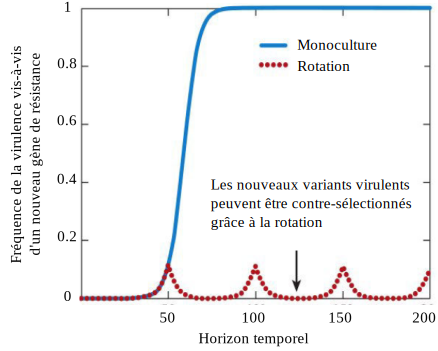
\includegraphics[width=0.8\linewidth]{rotation.pdf}
		\caption[Évolution  d’un agent pathogène vis-à-vis d'une plante porteuse d’un
		nouveau gène de résistance en monoculture  ou avec une rotation
		des cultures]{Évolution  d’un agent pathogène vis-à-vis d'une plante porteuse d’un
		nouveau gène de résistance en monoculture (courbe bleue), ou avec une rotation
		des cultures (courbe en pointillés rouges).  Adapté de \citep{Zhan2015}.
		}
		\label{rotation}
\end{figure}


%Dans les domaines de la santé publique et de l’agronomie, REX Consortium (2013) ont mis en avant l’intérêt des combinaisons entre mélange de molécules et leurs rotations dans le temps pour la gestion de la résistance conférée par les insecticides ou antibiotiques aux ravageurs et aux agents pathogènes, après avoir analysé un ensemble de 29 études théoriques sur le sujet. Ces études comparaient cette stratégie double (mélange et rotation) à des stratégies plus simples, consistant (i) en un mélange de molécules constant dans le temps, ou (ii) en une alternance temporelle entre différentes molécules utilisées une par une séparément, soit de manière cyclique, soit en changeant de molécule lorsque celle en cours d’utilisation était contournée. REX Consortium (2013) ont conclu que les stratégies combinant mélange et rotations étaient au moins aussi performantes, voire plus performantes que les autres stratégies pour retarder le contournement d’une résistance dans plus de 80~\% des comparaisons.
 Selon \citet{Zhan2015}, il existe encore trop peu d’études théoriques pour la conception et l’évaluation de stratégies  de gestion durable des maladies, notamment pour celles basées sur la rotation de \glspl{gene R} \citep{Fabre2015, Papaix2015, Lof2017, Rimbaud2018}. 
À partir d'une approche de modélisation, \citet{Fabre2015}  ont montré que les rotations et les mosaïques combinées  étaient plus bénéfiques que les mosaïques seules en termes de rendement lorsque des infections se déroulent majoritairement au sein d'une même parcelle, c'est-à-dire quand la capacité de dispersion de l'agent pathogène est faible, et pour des variants  où le contournement de la résistance vis à vis d'un virus se faisait après une seule mutation. Les auteurs ont aussi montré une augmentation de la durabilité des résistances grâce au maintien de  la fréquence des variants virulents sous un certain seuil.

	\citet{Rimbaud2018} ont trouvé que la rotation des cultivars peut être la plus efficace à long terme par rapport aux trois autres stratégies de déploiement (pyramidage, mélanges, mosaïques), une fois que tous les \glspl{gene R} ont été contournés. Cependant, ils ont montré que ce résultat dépend au moins en partie de la capacité de dispersion et de survie des agents pathogènes.  Un pathogène avec une grande capacité de dispersion aura tendance à diminuer l'efficacité de cette stratégie car le pathogène pourra se propager pour infecter d'autres champs. L'efficacité de la rotation   seule pourrait être limitée dans les régions où la culture est pratiquée sur de grandes superficies, en particulier pour les maladies propagées par voie aérienne.

%\tr{Je dois aussi présenter Zhu 2000 \citep{Zhu2000})}  
	 Certaines ont montré l’efficacité des rotations basées sur l'alternance de cultivars sensibles et résistants  pour lutter contre des pathogènes qui se dispersent peu, notamment contre les nématodes à galles \citep{McSorley2011, Miller2006, Tzortzakakis2000}. Une autre étude, menée sur la tomate en Espagne durant trois ans, a montré que cette alternance pouvait augmenter les rendements et la durabilité de la résistance des plantes  \citep{Talavera2009}. Quelques  études expérimentales ont évalué l'effet bénéfique des rotations pour différents types de pathosystèmes \citep{Zhu2000, Talavera2009, Djian-Caporalino2014, Burdon2014}. 

	 Au sein de notre laboratoire,  \citet{Djian-Caporalino2014} ont évalué et comparé expérimentalement sur trois ans  la  durabilité et l'efficacité de trois stratégies de déploiement des \glspl{gene R} chez le piment pour lutter contre les  nématodes à  galles \textit{Meloidogyne},  parasites telluriques peu mobiles :
le mélange de cultivars, les rotations  et le pyramidage de deux \glspl{gene R} dans un même cultivar. 
En s'assurant de l'absence  de virulence croisée, ils ont montré que l'alternance du \gls{gene R}  \textit{Me3} avec un autre \gls{gene R} à  mode d'action différent  \textit{Me1} chez le piment semble efficace pour réduire les populations de nématodes. Cette  efficacité pourrait reposer sur la spécificité de la virulence des gènes \textit{Me1 } et \textit{Me3},  démontrée en conditions contrôlées \citep{Djian-Caporalino2011} :  si une population peut contourner un \gls{gene R} (par exemple \textit{Me3} à résistance précoce), en revanche elle ne peut contourner un autre \gls{gene R} (par exemple le gène \textit{Me1} à résistance tardive).

%Les rotations  permettent d'éviter que les populations  ne soient soumises à des pressions de sélection constantes et n’évoluent rapidement vers la virulence (comme dans l'exemple de la \autoref{rotation}).

	
	Les nématodes à galles, évoqués à plusieurs reprises jusqu'ici, ont été choisi comme cas d'étude  dans cette thèse. Ils sont présentés  de façon plus détaillée dans la section suivante.

%\printbibliography[heading=subbibliography,segment=\therefsegment]

\section{Cas d'étude : les nématodes à galles } \label{nematode}

\subsection{Qu'est ce qu’un nématode ?}
	
\begin{figure}[h]
  \centering \includegraphics[width=1\linewidth]{schema_nem}
	  \caption[Schéma général d’un nématode]{Schéma général d’un nématode. \href{https://www.wormatlas.org/}{https://  
	  www.wormatlas.org/}}
	  \label{nematodes}
\end{figure}
	
	Les nématodes sont des vers ronds, non segmentés, filiformes et translucides (\autoref{nematodes}), qui appartiennent à l'embranchement des Nematoda, dont plus de 25000 espèces réparties  dans 20 ordres et 200 familles ont été identifiées jusqu'à présent \citep{Abad2008}.  Toutefois, on estime à plus d’un million le nombre d’espèces existantes de nématodes \citep{Hugot2001}. Ce sont des métazoaires. %tripoblastiques pseudocoelomates.
Dans le règne animal, ils représentent une grande partie de la biodiversité animale, juste après les insectes  qui constituent 80~\% de cette biodiversité. 
Ils s'acclimatent à pratiquement tous types d'environnements et sont donc distribués partout dans le monde. Les nématodes  ont réussi à s'adapter à de larges gammes d'écosystèmes et milieux : eau, sol, animaux, champignons, insectes et  plantes \citep{Bongers1998}. Certains d'entre eux participent de manière fondamentale à l'activité biologique dans divers écosystèmes. Ils jouent un rôle important dans la décomposition de déchets organiques, y compris dans la biodégradation de composés toxiques. La présence de nématodes dans les sols peut  même être un indicateur de la qualité du sol \citep{Yeates1987}.


\subsection{Les nématodes phytoparasites}
	
	Plus de  4500 espèces de nématodes phytoparasites ont été découvertes à ce jour \citep{Decraemer2006}.
Ils sont répartis dans deux ordres : celui des \textit{Dorylaimida} qui comprend les nématodes vecteurs de virus \citep{Maheswari1997} et celui des \textit{Tylenchida} qui est
l’ordre le plus important par le nombre d’espèces,  qui causent d'importants dégâts aux cultures \citep{DeGuiran1983}.
Ils mesurent tous  moins d'un millimètre de long et sont invisibles à l’œil nu.
La principale caractéristique des nématodes phytoparasites est un stylet perforant se situant dans la  partie antérieure du tube digestif. C’est une aiguille creuse
connectée à un système glandulaire hypertrophié, qui agit comme une véritable pompe en injectant des sécrétions nécessaires au parasitisme et en absorbant les nutriments
de la plante \citep{Abad2010}.  Les nématodes phytoparasites sont responsables de 11~\% de la perte de
production  des cultures vivrières \citep{Agrios2005}. Globalement, ils sont responsables de 10~\% à 20~\% de pertes de rendement sur toutes cultures confondues\citep{Raaijmakers2009}.
Les pertes annuelles mondiales seraient
estimées à plus de 100 milliards d’euros \citep{Sasser1987, Chitwood2003}. D'autres études menées 20 ans plus tard ont confirmé ces chiffres \citep{McCarter2009, Chitwood2003, Agrios2005}.
	
	De par leur comportement, il existe deux types de parasitisme : (1) les parasites aériens qui s'attaquent aux bulbes, tiges, feuilles, fleurs des plantes et (2) les parasites des racines qui peuvent être ectoparasites \footnote{se dit d'un parasite qui vit  à la surface des tissus végétaux, animaux ou humains} ou endoparasites, migrateurs  ou sédentaires.  

	Parmi les nématodes phytoparasites, les nématodes parasites des racines sont probablement la principale cause de pertes de récoltes, mais également ce sont  les plus représentés à l'échelle du globe \citep{Bird2003}.  Les nématodes phytoparasites des racines réalisent tout leur cycle de vie dans le sol et ne s’attaquent qu’aux
racines ce qui peut conduire à un dysfonctionnement du système vasculaire de la plante, voire à la mort de la plante selon le stade et les taux d’infestation. 
Les symptômes de l'infection par des nématodes des racines sont : 
	\begin{itemize}[label=--]
	\item des apparitions de galles ou de lésions racinaires qui favorisent d'autres pathogènes telluriques, fongiques 
	      ou bactériens ;
	\item une distorsion de la structure racinaire ou une augmentation du diamètre des racines ;
	\item une croissance racinaire réduite (perte racinaire) ou une  nécrose des racines pouvant entraîner la mort de 
	     la plante.
	\end{itemize}
Par exemple, les nématodes  endoparasites migrateurs pénètrent complètement et se déplacent dans les tissus parasités  des racines entraînant des lésions (genre : \textit{Ditylenchus, Pratylenchus, Rotylenchus}). Les nématodes endoparasites sédentaires pénètrent dans les tissus et se sédentarisent pour établir un site nourricier pour leur développement, entraînant la formation à terme de galles ou de kystes.

La majorité des pertes de récoltes sont causées par les nématodes endoparasites sédentaires, qui comprennent les nématodes à kystes (genres \textit{Heterodera, Globodera})  \citep{Perry2018} et les  nématodes à galles (genre \textit{Meloidogyne}) \citep{Perry2009}, ainsi que les endoparasites migrateurs, qui comprennent par exemple les nématodes à lésions des racines (genre \textit{Pratylenchus}) \citep{Mass1998}. 
 
\subsection{Les nématodes à galles du genre \textit{Meloidogyne}}
	
	Les nématodes à galles du genre \textit{Meloidogyne} sont des endoparasites obligatoires des racines. Du fait de leur taille microscopique et de leur présence au sein même des racines, ils sont longtemps passés inaperçus.  Ils créent des galles au niveau des racines, entraînant une déformation importante du système vasculaire  de la plante, mais aussi  un dépérissement des parties aériennes et parfois la mort de plante.

	Ils sont particulièrement nuisibles économiquement aux cultures agricoles du monde entier en raison de leur large gamme d'hôtes, comprenant plus de 5500 espèces de plantes \citep{Blok2008}, et de leur large répartition géographique \citep{Jones2013}.  En cas d’infestation forte, les galles peuvent envahir tout le système racinaire, ce qui provoque une diminution des rendements de la plante  et  peut conduire dans certains cas à la perte totale d’une récolte. En effet, les racines attaquées par les nématodes ne sont plus capables d’extraire correctement des nutriments du sol et donc de se développer (\autoref{degat}).  Les dommages  de certaines espèces de \textit{Meloidogyne} ont été répertoriés par \citet{Greco2010} et \citet{Wesemael2011}.  Par exemple, des pertes de rendement de 62 à 100~\% ont été signalées en culture de tomates sensibles  \citep{Seid2015, Gine2017}, 30 à 60~\% en cultures d'aubergine, 50~\% pour le melon,  37~\% à 50~\% pour la  pastèque \citep{Sikora2005} et 88~\% pour les concombres \citep{Gine2017}. 
En Europe, ils sont responsables de dégâts atteignant 10\% de la production céréalière et ils  entraînent des diminutions de récoltes de 20 à 30\% dans les vergers d'agrumes méditerranéens \citep{Feldmesser1971}.  Dans le sud-est de la France,  plus de 40\% des exploitations maraîchères sont touchées \citep{Djian-Caporalino2010, Djian-Caporalino2012}.
Le changement climatique est susceptible d'influencer nettement  la distribution de ces parasites et par conséquent d'accentuer les pertes de rendement des  cultures \citep{Bebber2014}. 

	\begin{figure}
	    \centering
		  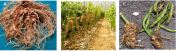
\includegraphics[width=0.9\linewidth]{degat}
		  \caption[Dégâts provoqués par \textit{ Meloidogyne incognita}]{Dégâts provoqués par \textit{ Meloidogyne 
		   incognita} sur : \textbf{A} des racines de tomates ;
		   \textbf{B}  une culture en serre d’aubergines ; \textbf{C} 
		   des racines de haricots.}
		  \label{degat}
	\end{figure}

	Plus de de 90 espèces ont été décrites \citep{Jones2013, Blok2008}, dont 23 en Europe \citep{Wesemael2011}, mais seulement quatre d'entre elles sont considérées comme particulièrement nuisibles : \textit{M.~incognita, M.~arenaria, M.~javanica} et  \textit{M.~hapla}. En France, on retrouve principalement les trois premières de ces quatre espèces.  Ces trois espèces sont à reproduction parthénogénétique mitotique   (c'est à dire à reproduction clonale) \citep{Triantaphyllou1985}. Elles sont responsables de
la majorité des pertes de rendement des cultures maraîchères causées par les
nématodes \citep{Sikora2005}. Elles sont également largement répandues dans les régions tropicales, où elles s’attaquent aux cultures de
bananier, de café, de coton de canne à sucre ou encore d’ananas \citep{Sikora2018}. Elles  prospèrent dans les sols des contrées à climat chaud et hivers courts.

	L'espèce \textit{Meloidogyne incognita} est   l'une des espèces les plus largement répandues à travers le monde et celle qui cause le plus de dégâts. \textit{M.~incognita} se distingue par son caractère extrêmement polyphage. Elle attaque plus de 200 espèces végétales, dont les tomates, aubergines, poivrons, pommes de terre, melons, concombres, laitues, chicorées, haricots, carottes, \textit{etc.} 
	Dans ce contexte, certains auteurs indiquent que \textit{M. incognita} serait l'un des parasites de plantes parmi les plus préoccupants au monde \citep{Bebber2014}. 	
	

\subsection{Le cycle de vie du nématode \textit{M. incognita}}
\label{sec:cycle}
 
 
Le cycle biologique  du nématode se déroule en  deux phases décrites ci-dessous.

\paragraph{La phase exophyte}

	Les œufs sont produits dans une matrice gélatineuse à la surface des racines.  Chaque œuf présent dans le sol libère directement une larve de deuxième stade (J2),  la  mue J1--J2 ayant lieu dans
l’enveloppe de l’œuf. Les larves ont une apparence vermiforme et sont la plupart du temps translucides ou de couleur claire. Elles sont mobiles dans le sol et, attirées par les
exsudats racinaires, elles pénètrent à l’intérieur de leur hôte. On parle aussi de stade infestant ou de larves infestantes \autoref{larve}.

	\begin{figure}
	  \centering
		  \includegraphics[width=0.7\linewidth]{J2}
		  \caption[Larve de deuxième stade de \textit{M. incognita}]{\textbf{A}  Schéma de la partie antérieure d’une   
		          J2 de \textit{Meloidogyne} d’après \citet{Vanholme2004}.
		           Stades de développement  de \textit{M. incognita}. \textbf{B} Juvéniles du deuxième stade  
		           \textit{M.incognita} observées à la loupe binoculaire (source : photos Inrae Sophia Antipolis).}
		 \label{larve}
	\end{figure}

\paragraph{La phase endophyte}
Cette pénétration a lieu préférentiellement au niveau de l’apex (extrémité) des racines en croissance et constitue le début d'une phase où le nématode va se sédentariser dans les racines de la plante entre le 3 ième et le 4 ième jours. En effet,  les larves J2 migrent dans la racine pour remonter vers le cylindre central de la plante et initier un site nourricier potentiel. Les J2 instaurent un site nourricier composé en général de 5 à 6 cellules géantes plurinucléées \footnote{se dit d'une cellule qui renferme plusieurs noyaux}  pour les assister dans leur parasitisme, en sécrétant des salives  et d’autres métabolites. 
Une fois établi, le parasite n'a plus besoin de se déplacer pour accomplir son cycle \citep{Abad2010}. Grâce à son stylet buccal, il ponctionne les cellules géantes et aspire leur contenu pour se nourrir.
%Cette larve J2 subit alors deux mues successives qui la mènent au troisième (J3), puis au quatrième stade larvaire (J4). 
		
	 Après 3 mues, les larves J3 puis J4 deviennent des femelles matures qui  produisent alors une masse d’œufs gélatineuse à l'extérieur de la racine.
Chaque femelle peut produire environs un millier d’œufs \citep{Castagnone-Sereno2013}, qui vont démarrer un nouveau cycle.
%Plus précisément dans le cadre de cette thèse,   nous nous sommes basé sur des publications dans lequel le potentiel reproducteur d'une femelle \textit{Meloidogyne incognita} pouvait être compris entre 250 et 300 œufs \citep{Castagnone-sereno2007, Djian-Caporalino2011}. 
Le cycle complet  (\autoref{cycle}) s’effectue en moyenne entre  20 à 24 jours à 25$^{\circ}$. Le cycle peut durer jusqu'à 40 jours selon la température.
Chez les espèces \textit{M. incognita} qui sont à reproduction  parthénogénétique, les mâles peuvent être très rares et ne participent pas à la reproduction \citep{Triantaphyllou1979}. La présence des mâles est plus élevée lorsque  les  J2 sont confrontées à des conditions défavorables de développement (\textit{e.g.} mauvais état des racines nourricières de la plante hôte). 
Contrairement aux J2 et femelles, les mâles ne se nourrissent pas et quittent la racine. Par ailleurs, le taux d’éclosion de l’espèce \textit{M. incognita} peut être total dans les conditions environnementales optimales. Mais il est en généralement  compris entre 60~\% et 80~\% dans les conditions expérimentales \citep{DeGuiran1979}. %Par exemple, nous avons constaté
%que dans les conditions expérimentales de l'Ehwaeti et al \citep{Ehwaeti1998} que le taux d’éclosion était de 73~\% \citep{Ehwaeti1998}.
%Nous avons donc déduit que la femelle pond 17 oeufs viables en moyenne au cours de sa durée de vie, qui est comprise entre 8 à 10 jours (Ekanayake and Vito, 1986).
La survie naturelle  dans le sol en absence de nourriture à 25 $^\circ$ C est de 25 jours, les J2  mobilisant l’ensemble de leurs réserves énergétiques avant de mourir \citep{Tsai2008}.
Les population de \textit{M. incognita} peuvent néanmoins se maintenir en infectant
les adventices hôtes ou des débris de racines dans le sol.
Enfin, les œufs  peuvent survivre des semaines ou des  mois  $via$ des stratégies telles que le retard de l'embryogenèse, la diapause ou encore des états de quiescence qui prolongent leur viabilité \citep{Perry2009}. 


\begin{figure}
	\centering \includegraphics[width=0.8\linewidth]{cycle_de_vie3}
		\caption[Cycle de vie du nématode à galles \textit{Meloidogyne} \textit{incognita} dans une racine (Photos  
		Inrae Sophia Antipolis).]{Cycle de vie du nématode à galles \textit{Meloidogyne} incognita dans une racine.  La 
		larve juvénile mobile de deuxième stade  (J2)
      	migre après 24h  en moyenne vers l'extrémité d'une racine (A)  avant de remonter le long du cylindre central au  
      	bout de trois jours (B) et atteindre l’emplacement du futur site nourricier (C-C').
	    Les stades juvéniles J3  et J4  fixés sont visibles en coupe racinaire avec les cellules géantes (*)  au bout 
	    du 10 ième et 14 ième jours respectivement (D-E).% Ces troisième et quatrième stades larvaires  ne se nourrissent pas et n’ont pas de stylet.
	    La larve (J4) muent alors une dernière fois pour produire un adulte, soit  mâle (F) ou femelle (G). La femelle 
	    mature est visible au  bout du 20 ième jour et produit une masses d'oeufs  à l'extérieur de la racine au bout 
	    du 24 ième jour (H). Adapté de \citet{Abad2008}.}
	   \label{cycle}
\end{figure}

\newpage
 
\subsection{Moyens de lutte} \label{lutte}
	
\subsubsection{La lutte chimique}

	La lutte contre les nématodes à galles a longtemps été restreinte  à l'utilisation de produits chimiques.
Tout d'abord, on retrouve  des gaz toxiques (fumigants), tels que des produits
organo-halogénés (bromure de méthyle, 1,3-dichloropropène) ou de la famille des
thiocyanates (métham-sodium, dazomet) \citep{Wesemael2011}. Ensuite, il existe  des nématicides systémiques (non-fumigants) tels que
des carbamates (aldicarbe, oxamyl, carbofuran) ou des organophosphorés (éthoprophos,
phénamiphos, fosthiazate, terbufos) \citep{Cavelier1987}. Ces produits qui se diffusent par la sève, tuent le nématode par ingestion. Toutefois, ils sont interdits sur toute culture comestible.

	L'utilisation de ces produits chimiques n'était efficace que sur de faibles profondeurs et ils n'étaient donc pas efficaces dans les couches profondes du sol.
Depuis 2006, beaucoup de ces produits chimiques ont été retirés du marché à cause de leur impact environnemental et sanitaire \citep{Abad2010}. C'est par exemple le cas du  bromure de méthyle qui a été interdit par l'UE \citep*{MBTOC2006, ECDirective2009}. 

\subsubsection{Prophylaxie et lutte physique}
		
	 La prophylaxie (hygiène des parcelles) consiste d'une part à  enlever un maximum de déchets et de racines pour que les parasites évitent de trouver de quoi se nourrir et d'autre part à détruire les adventices aux abords des parcelles, les mauvais herbes constituant un réservoir pour la multiplication des nématodes. D'autre moyens, physiques, sont utilisés pour nettoyer les sols  comme la solarisation  (\autoref{solarisation}). C'est un procédé qui consiste à inonder le sol  puis à le   recouvrir d'une bâche plastique transparente    afin de permettre de faire monter sa température jusqu’à 50$^{\circ}$C selon le principe de l'effet de serre  \citep{Porter1983}.
	
	\begin{figure}
		\centering \includegraphics[width=0.8\linewidth]{solarisation.jpg}
		\caption{Solarisation en plein champ et sous abri (photo GRAB).}
		\label{solarisation}
	\end{figure}
	
	Si cette technique a démontré son efficacité pour le contrôle des agents pathogènes fongiques,  utilisée seule elle est  peu efficace  contre les nématodes à galles et doit être renouvelée tous les 2-3 ans \citep{Anastasiadis2008}. Si la température n’est pas assez élevée en profondeur, dans certains cas (petites surfaces, sols sableux, équipement disponible), on peut utiliser la désinfection à la vapeur. Celle-ci permet d’injecter de la vapeur sous une bâche étanche recouvrant le sol pendant 1h30 à 3h. La profondeur traitée est de dix à vingt centimètres lorsque le sol est finement préparé. Cette méthode est néanmoins coûteuse et polluante (fluel).
%	\begin{figure}
	%	\centering \includegraphics[width=0.8\linewidth]{desinfection-vapeur.png}
		%\caption{ Désinfection à la vapeur (photos Inra Sophia Antipolis).
		%}
		%\label{solarisation}
	%\end{figure}
	
	
\subsubsection{La lutte culturale} \label{lutte:culturale}
		
	La lutte culturale est une méthode de lutte  qui vise à limiter le développement des parasites/pathogènes  en jouant sur leur environnement naturel et en perturbant leur cycle biologique. Elle peut inclure, de manière non exhaustive,  la gestion de l'irrigation, les rotations culturales, les plantes pièges.
La gestion de l'irrigation permet d'éviter la dissémination des nématodes par ravinement et donc une meilleur protection des cultures au champs. Le labour  profond estival peut
permettre de faire remonter les  nématodes des couches profondes du sol qui vont
sécher en surface. Néanmoins, un labour systématique a pour conséquence une diminution de la quantité de matière organique du sol.
Les rotations culturales bien réalisées jouent un rôle important dans la lutte contre les nématodes. 
Pour freiner le développement des nématodes on peut inclure dans les rotations des espèces végétales
mauvais hôtes vis-à-vis des nématodes à galles ($e.g.$ \textit{Liliaceae}, \textit{Brassicaceae}),  biofulmigantes ($e.g.$ sorgho,  \textit{Brassicaceae}) ou des  plantes pièges ($e.g.$ radis fourragers) en interculture \citep{Djian-Caporalino2019}. 
Les  plantes biofumigantes  produisent des phytoanticipines qui agissent comme
des inhibiteurs de développement ou des toxines. La culture de plante pièges consiste à planter un bon hôte pendant une courte période, suffisante pour assurer une forte pénétration des nématodes et un développement du nématode.  Ensuite, les racines doivent être enlevées ou détruites afin de tuer les nématodes avant la reproduction (dans le cas de plantes pièges résistantes la culture n'est pas détruite en générale ce qui n'est pas le cas de cultures sensibles). Par exemple,  certaines variétés de piments et melons 
  vont  attirer les  nématodes  et permettent la pénétration des larves de \textit{Meloidogyne} mais pas leur développement en femelles fécondes \citep{Berge1974, Djian-Caporalino2008}. L'utilisation de ces plantes de service fait l'objet de récents projets \citep{Djian-Caporalino2019}.
	
	


%4.2. Lutte biologique

%Certains antagonistes du sol tels que les bactéries et les champignons prédateurs peuvent être utilisés comme agents de lutte biologique contre les nématodes (Ritter, 1985 ; Robinson, 1999). Ce type de pratique présente cependant la difficulté de maintenir un auxiliaire dans un sol qui ne lui convient pas toujours. Cette méthode de lutte est donc très loin d’être appliquée à grande échelle.

	
\subsubsection{La lutte génétique}


	\begin{figure}[H]
		\centering \includegraphics[scale=0.4]{RvsS.pdf}
		\caption[Comparaison de
l’interaction des nématodes
à galles entre une plante
sensible et résistante]{ Comparaison de
l’interaction des nématodes
à galles avec A) une tomate
sensible B)  et une tomate
résistante   \textit{Mi-1}, C) un piment résistant \textit{Me1}  (photos
INRAE Sophia Antipolis).  Adapté de \citet{Djian-Caporalino2015}.}
 		\label{RvsS}
	\end{figure}




	La résistance qualitative ou totale est une méthode  efficace, respectueuse de l'environnement et économiquement viable dans la lutte contre les nématodes  du genre \textit{ Meloidogyne} \citep{Roberts1982, Roberts1990, Roberts1993, Williamson2009, Davies2015, Barbary2015}. Les mécanismes d'interaction du modèle gène pour gène, qui se traduit par un \gls{HR} en cas d'interaction incompatible (\autoref{RvsS}),  ont été décrits pour les nématodes à galles \citep{Kombrink2001, Pegard2005, Williamson2006}. Le nématode, une fois dans les racines, produit des substances chimiques  reconnues spécifiquement par un \gls{gene R} de la plante.


	Cependant, l'utilisation de la résistance aux nématodes  à galles se heurte à plusieurs problèmes. Tout d'abord, à
	ce jour, seulement une trentaine de  gènes de résistance vis-à-vis des différentes espèces de \textit{Meloidogyne}  ont été identifiés (\autoref{tab:resistance}). En particulier, il existe peu de résistances naturelles conférant une résistance totale aux nématodes à galles   :  la
carotte (gène \textit{Mj-1}), les prunus (gènes \textit{Ma}), la tomate
(gènes \textit{Mi}), la pomme de terre (gènes \textit{Rmc1},
\textit{MfaXII}),  le coton (gènes \textit{MIC-3,
rkn-1, Mi-1}), les piments/poivrons (gène \textit{N} et
gènes\textit{ Me} ) \citep{Djian-Caporalino2008}.
%La plupart  des cultivars  ont été obtenus par introgression  d'un nombre limité de cultivars naturellement résistants ou de portes-greffes \og  courges \fg{}  apportant plus de vigueur aux Cucurbitacées.

\begin{table}
	\caption[Résumé des gènes de résistance aux nématodes à galles]{Un résumé des gènes de résistance aux nématodes à  
	 galles (\textit{Meloidogyne}),  d'après \citet{Williamson2009}.}
	\centering
	\begin{tabular}{c}
	\includegraphics[width=1\linewidth]{tab_res.pdf}\\
	\end{tabular}
	\label{tab:resistance}
\end{table}

	
	Ensuite, les résistances peuvent être contournées par des populations  de \textit{Meloidogyne} qui évoluent plus ou moins rapidement \citep{Castagnone-Sereno2002, Verdejo-Lucas2009,Jarquin-Barberena1991}.  
Pour mettre en évidence, ce succès parasitaire surprenant malgré l'absence de recombinaisons sexuels et génétiques de nombreuses études expérimentales  ont travaillé sur ces questions de contournement.
Premièrement, la virulence des nématodes à galles  vis-à-vis d'un gène de résistance pourrait être due  à des  variations nucléotidiques entre
nématodes avirulents et virulents 
\citep{Neveu2003, Semblat2001}.Deuxièmement,
des chercheurs se sont intéressés  aux variations des copies de gènes dans les régions du génome d'un variant virulent comparativement à celui d'un variant avirulent pour tenter d'expliquer l'apparition du variant virulent \citep{Castagnone-sereno2019}. Leur étude a montré qu'il existe des régions du génome uniquement représentés chez les lignées avirulentes et absent sur les lignées virulentes. Ainsi, la perte de gènes chez le variant virulent  pourrait être un élément clef dans l'acquisition de la virulence. Ces résultats et/ou également  d'autre facteurs génétiques telles des  inversions, des translocations ou des éléments transposables  dans le génome de \textit{Meloidogyne}  pourraient expliquer l'apparition du variant virulent. Troisièmement, des chercheurs de notre laboratoire soupçonnent que des modifications épigénétiques  pourraient provoquer des modifications au niveau du génome qui sont connus aujourd'hui pour être des facteurs déterminants dans l'acquisition de nouveaux traits.
	
	 Cependant, on connaît très peu de choses sur les modifications génétiques et épigénétiques impliquées dans l'acquisition de la virulence chez \textit{Meloidogyne} 
De ce fait,  le taux de mutation des nématodes \textit{M.} \textit{incognita} reste encore inconnu. À titre d'exemple, le taux de mutation du nématode \textit{C. elegans}  est  de l'ordre de  10$^{-6}$ \citep{Denver2004}. 
En revanche, le taux d'apparition d'individus virulents dans une population avirulente (ou  la fréquence d'apparition de phénotype virulent dans une population avirulente)  serait plus proche de  10$^{-3}$ \citep{Castagnone-Sereno1994}.
	 
	 Le problème du contournement  est particulièrement préoccupant pour le gène de la tomate \textit{Mi-1} qui est à l'heure actuelle le seul  présent dans toutes les variétés de tomates commercialisées dans le monde. Pour cette raison, un changement de variété au cours du temps ne modifierait pas la pression de sélection appliquée sur les populations de parasites, puisque \textit{in fine} le gène de résistance resterait le même. 
L'étude de la sélection vers  la virulence a été menée dans  l'interaction entre \textit{M. incognita} et la tomate résistance \textit{Mi-1}  \citep{Castagnone-Sereno2002, Castagnone-Sereno2007}. Le contournement de ce gène a donc été mis en évidence, ce qui remet potentiellement en question la durabilité de cette méthode \citep{Castagnone-Sereno2002}.
 
 
	 
	L’analyse des traits d’histoire de vie des nématodes, lorsque les nématodes  sont inoculés à des génotypes sensibles ou résistants, montre qu’il existe un coût  associé à l'acquisition de la virulence. En effet, la virulence chez les nématodes \textit{M. incognita} est  associée à un coût de fitness sur les plantes sensibles, représenté par une diminution de la reproduction et de la fertilité \citep{Castagnone-Sereno2007, Djian-Caporalino2011} (\autoref{cost}). Ainsi, si les nématodes virulents sont sélectionnés en cas d'usage de plantes résistantes, ils sont aussi contre-sélectionnés en cas d'usage de plantes sensibles au profit de nématodes avirulents.
Dans l'étude de  \citet{Castagnone-Sereno2007}, les coûts de virulence peuvent être calculés selon la formule suivante :
\begin{equation}
 Ch(\%) = 1-RP_v/RP_{av} 
 \end{equation}
où $RP_v$ est le potentiel reproducteur  (nombre d’œufs / nombre de larves inoculées) de la lignée virulente et $ RP_{av} $  est le potentiel reproducteur  de la lignée avirulente  sur tomate sensible  \citep{Castagnone-Sereno2007}. 
À partir de cette formule, nous avons estimé le coût de virulence sur tomates sensibles
à 31~\%  pour la reproduction  et  à 9~\% pour la fertilité.

\begin{figure}
	\centering 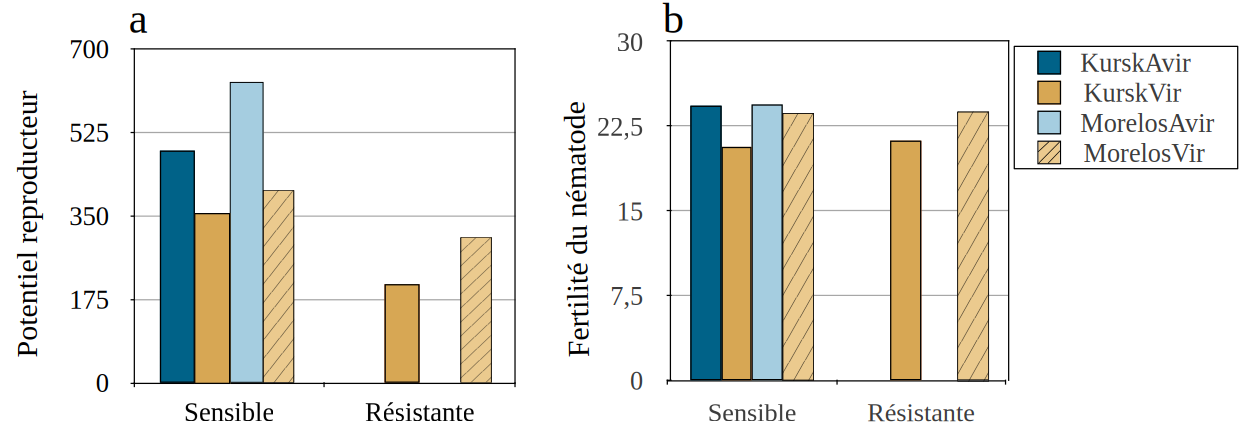
\includegraphics[width=1\linewidth]{cost2.pdf}
	\caption[a) Potentiel reproducteur et b) fertilité des nématodes \textit{Meloidogyne} \textit{incognita}. ]{ a)  
	 Potentiel reproducteur (nombre d'oeufs viables / larves inoculées) de M. \textit{incognita} sur tomates sensibles  
	 (\textit{cv.} Saint Pierre) et \textit{Mi} résistantes (\textit{cv.} Piersol). b) Nombre de femelles de M. 
	 \textit{ incognita} ayant produit une ponte par larve inoculée  sur plantes sensibles et résistantes. KurskAvir et 
	 MorelosAvir représentent les lignés avirulentes ; KurskVir et MorelosVir représentent les lignés virulentes.   
	 Adapté de \citet{Castagnone-Sereno2007}.}
	\label{cost}
\end{figure}



	
	En conclusion, des solutions alternatives à la lutte chimique existent (solarisation, biofumigation, désinfection vapeur, plante piège), mais prises individuellement elles, restent insuffisantes en termes d’efficacité  pour une augmentation significative des rendements. La résistance des plantes est une stratégie efficace et peu coûteuse pour le contrôle des nématodes à galles. La réponse immune des plantes est principalement représentée par les \glspl{gene R} dans le cas des nématodes à galles  dont l’utilisation est de plus en plus compromise à cause du nombre limité de
variétés résistantes et de la faible durabilité de certains \glspl{gene R}.
Il paraît plus que nécessaire de  mettre l'accent sur des études qui suggèrent une gestion plus durable du nombre limité et irremplaçable de résistances encore disponibles vis-à-vis des nématodes à galles.

\textit{
Dans cette thèse, nous avons identifié des rotations de cultures sensibles et résistantes pour augmenter les rendements, mais également pour préserver les rares et précieux \glspl{gene R} disponibles.}

%Dans l'infection par les nématodes, il existe différents types de réponses  des résistances chez les plantes. Notamment, chez le piment il existe deux gènes
%majeurs de résistance aux nématodes à mécanismes d’action différents (\autoref{RvsS}) : l’un (\textit{Me3}) agit de manière
%précoce et l’autre (\textit{Me1}) de manière plus tardive. Dans la suite, nous aborderons la spécificité de ces modes d'action dans le pathosystème piment-\textit{Meloidogyne} et leur lien avec la durabilité des \glspl{gene R}. 
\newpage
\subsection{Les gènes majeurs de résistance \textit{Me(s)} du piment aux nématodes à galles}

\label{sec:gene-R-piment}

\begin{encadre2}{Le piment : origine}
\label{pim}Le terme vernaculaire \og piment \fg{} regroupe l’ensemble des plantes du genre \textit{Capsicum} appartenant à la même famille des \textit{Solanaceae} que la tomate, la pomme de terre, l’aubergine et le tabac. Le genre regroupe environ vingt-cinq espèces différentes avec des différences au niveau de la forme, de la couleur du goût, de la puissance du piquant et de la taille.

\parbox{7cm}{%
\begin{figure}[H]
\hspace{3.5cm}
\includegraphics[width=0.4\linewidth]{piment.png}	

 \begin{minipage}{0.96\linewidth}
 \caption[Collection de piments de l’INRAE d’Avignon, France (Photos Inrae sophia Antipolis)]{Diversité 
      de formes et couleurs de fruit chez \textit{C.}  \textit{annuum} (échantillon de la collection de 
  piment de l’INRAE d’Avignon, France) }
 \label{piments}
 \end{minipage}	
\end{figure}
}
Parmi elles, seules cinq ont été domestiquées :
\textit{Capsicum annuum, C. frutescens, C. chinense, C. pubescens} et \textit{C. baccatum.}
Le piment a été domestiqué pour la première fois en Amérique.
Des traces archéologiques ont montré que  les piments font partie de l'alimentation des peuples d'Amérique depuis au moins 8000 ans \citep{Aguilar-Melendez2009}. L'introduction de l'espèce \textit{C. annuum} en Europe pour la première fois date du XVe siècle, lorsque Christophe Colomb le ramena de son
premier voyage. Cette espèce est maintenant la plus cultivée au monde 
Il s’agit d’une culture maraîchère qui produit des petits fruits forts et « brûlants »
ainsi que des fruits plus gros et doux couramment appelés \og poivrons \fg . Cette espèce est originaire
du Mexique, du Sud de la Bolivie et du Brésil, on la retrouve maintenant dans les régions tropicales à travers le monde et dans les pays méditerranéens.
%\begin{figure}
	%\centering \includegraphics[scale=0.15]{origine.png}
	%\caption{Aires d’origine et de domestication présumées pour les 5 espèces cultivées de
%piment}	
%\end{figure}
\end{encadre2}	


	En 1983, \citet{Hendy1983}, mettent en évidence de nouvelles sources de résistance vis-à-vis des nématodes 
à galles  à travers l’étude de la collection d’accessions de piment de l’INRAE
d’Avignon (\autoref{piments}). Deux lignées de \textit{C. annuum} génétiquement très différentes se révèlent hautement résistantes aux  principales espèces de \textit{Meloidogyne}.

	 Il s’agit de PM687, lignée  originaire de l’Inde, et de PM217, une lignée  originaire d’Amérique. Par la suite, une troisième lignée de \textit{C. annuum} très résistante aux nématodes à galles a été
mise en évidence \citep{Djian-Caporalino1999}. Il s’agit de PM702, lignée issue d’une
variété  originaire du Mexique \gls{CM334}.
À travers plusieurs   études de ces trois lignées hautement résistantes,  de nombreux  \glspl{gene R} ont été mis en évidence  (\autoref{fig:Me}).
Ces gènes, nommés gènes\textit{ Me}, agissent de manière indépendante dans une relation \og gène-pour-gène  \fg{} et sont stables à haute température \citep{Dalmasso1985, Djian-Caporalino1999, Djian-Caporalino2001, Djian-Caporalino2007}. 
Trois de ces gènes majeurs,  \textit{Me1, Me3 et Me7},  ont un large spectre d’action et contrôlent la résistance vis-à-vis des principales espèces de \textit{ Meloidogyne: M. arenaria, M. incognita, et M. javanica}.
%Les gènes \textit{Me1, Me3 et Me7} chez le piment, qui  contrôlent les espèces\textit{ M. incognita, M. arenaria et M.
%javanica}  restent efficaces %au-dessus de 30$^\circ$ C. À titre d'exemple,  le gène \textit{Mi} de la tomate  contrôlant ces mêmes espèces est inefficace  à partir de 32$^\circ$ C (Ammati1986).
%Les gènes de résistance \textit{Me1, Me3} ont été par   ,et  le gène\textit{Me7}) a été mis en évidence par.


\subsubsection{Comparaison des modes d'action des gènes \textit{ Me(s)}} 
\label{sec:compR-gene-piment}
	Les gènes de résistance \textit{Me1} et \textit{Me3 } ont montré des différences dans leur mode d'action en réponse aux nématodes  \textit{M. incognita} \citep{Blevezacheo1998, Pegard2005}. \textit{Me3 } (comme le gène \textit{Mi-1} de la tomate) agit très précocement bloquant
le nématode dans le cortex de la racine et, des réactions d'hypersensibilité sont observées au niveau
de l’épiderme ou du cortex. \textit{Me1}
induit une réponse plus tardive, permettant la pénétration et la migration du nématode dans la racine
jusqu’au cylindre central, mais empêchant le développement normal des cellules géantes qui finissent par se nécroser, entraînant la mort du nématode qui ne peut plus se nourrir. 
 
\begin{figure}
	\centering 
	    \includegraphics[width=0.8\linewidth]{M(e).png}
		\caption[ Base génétique de la résistance des lignées de piment étudiées
		     pour les principales  espèces de \textit{ Meloidogyne}.]{ Base génétique de la résistance des lignées de 
		     piment étudiées pour les principales 
		     espèces de \textit{ Meloidogyne}. D'après \citet{Djian-Caporalino2015}.
		}
		\label{fig:Me}
\end{figure}

\subsubsection{Lien entre mécanisme de défenses et contournement des résistances majeurs} \label{sec:mécanisme-contournement}

	
	D'après \citet{McDonald2002}, le risque de contournement des \glspl{gene R} par les nématodes devrait être faible : taux de multiplication faible, cycle biologique long, reproduction à parthénogenèse mitotique, faible capacité de dispersion \citep{Triantaphyllou1985}.
Pourtant , des nématodes virulents  ont été observés en fonction du mécanisme de défense impliqué chez les gènes majeurs.
Par exemple, le gène de résistance, \textit{Me3} (résistance à hypersensibilité précoce),   semble être facilement contournable \citep{ Pegard2005, Djian-Caporalino2011, Djian-Caporalino2014}, tout comme le gène \textit{Mi-1} de la tomate \citep{Castagnone-Sereno2002}. En revanche, le gène \textit{Me1}  (résistance à hypersensibilité tardive) est plus difficilement contournable, même si des contournements ont été observés quand le  gène est introgressé dans un fond génétique sensible \citep{Barbary2014}.  
 On suppose que la forte durabilité de ce \gls{gene R} serait liée au fait que les réactions d'hypersensibilité  provoquées plus profondément dans la racine bloqueraient irréversiblement le développement de tout autre génotype de nématode, empêchant ainsi la sélection d'un génotype virulent \citep{Pegard2005}. On peut légitiment se poser une question sur  un potentiel effet de ces deux modes d’action de la résistance sur la compétition  des populations avirulentes et virulentes ? Dans de nombreux pathosystèmes, la co-infection d'hôtes  par de multiples eucaryotes
sont très couramment observées chez les espèces parasitaires naturelles
et une  littérature importante s'est crée
sur les conséquences épidémiologiques et évolutives  \citep{Alizon2013, Viney2013, Zhan2013}.
La compétition entre les génotypes d'agents pathogènes pour des ressources d'hôtes limitées peut avoir un impact important sur l'évolution des agents pathogènes. 

 	\begin{figure}
	\centering \includegraphics[scale=0.3]{contournement.png}
		\caption[Lien entre mécanisme de défenses et contournement des résistances majeurs]{Lien entre
		différents types de mécanisme de résistance de 2 gènes majeurs chez le piment 
		 et possibilité
		de contournement des
		gènes de résistance, jours après inoculation (\glsname{jai}). Adapté de \citet{Castagnone-sereno2001,Pegard2005} et \citet{Djian-Caporalino2011}.}
	\end{figure}

	Pour tenter de répondre à cette question il serait souhaitable d’étudier un modèle
prenant en compte la réponse d'une résistance tardive  et la comparer à celle d'une résistance précoce.
Ces modes d'action différentiels de la plante résistante liés à la capacité des pathogènes à
contourner ou pas les gènes impactent potentiellement la durabilité des résistances.  En effet, un gène facilement contournable ne  devrait pas être déployé tous les ans alors qu'un gène difficilement contournable pourrait être déployé sur un plus long terme.

\textit{Dans cette thèse, nous nous sommes également  intéressés  à savoir comment ces différents modes d'action (précoce et tardif) impactent  la durabilité des \glspl{gene R}.
}

\section{Structure de la thèse}

	L'objectif principal de cette thèse est de concevoir et d'évaluer les différents scenarios de déploiement
des résistances variétales et des pratiques agronomiques pour gérer durablement les populations de
nématodes à galles en cultures maraîchères. %Les
%expérimentations étant difficilement réalisables à très long terme (et à l'échelle des exploitations), la
%modélisation est alors un outil intéressant pour étudier les résistances des plantes dans des stratégies de déploiement à ces échelles. 
Ce projet vise donc  au développement d’un nouveau cadre de modélisation, adapté aux spécificités du pathosystème étudié.  Il repose sur une utilisation importante de simulations numériques, ce qui a nécessité
des moyens de calcul intensif. Mes travaux se situent à l’interface de la modélisation mathématique  en épidémiologie et de l’écologie parasitaire.  Cette approche innovante repose sur : 
\begin{itemize}
\item  la construction d'un modèle représentatif des dynamiques saisonnières de nématodes à galles
à l'échelle de la parcelle et son ajustement à des données expérimentales issues de la littérature \citep{Ehwaeti1998};
\item  la recherche des stratégies optimales de déploiement d'un \gls{gene R}, combiné à des
pratiques agronomiques, et l'évaluation de la robustesse de ces stratégies;
\item l'estimation du taux de mortalité et la calibration du modèle grâce à des données d'une expérience \textit{in vivo} réalisée au cours de la thèse décrivant la dynamique d'infection de plantes sensibles par des nématodes à galles (\textit{M. incognita}).
%\item %la comparaison des stratégies optimales de déploiement de cultures résistantes et leur durabilité pour deux gènes R majeurs chez le piment, en fonction des capacités de contournement de la
%résistance par les nématodes.
\end{itemize}
L'étude des processus évolutifs, écologiques et épidémiologiques agissant sur
la durabilité des \glspl{gene R}  contre les nématodes à galles pourrait permettre de formuler  des recommandations  quant aux
pratiques agricoles qui favorisent la durabilité des résistances et  également de renforcer les processus de création et de sélection variétale. \\

Le manuscrit de thèse est organisé en 5 chapitres, avec le chapitre introductif :\\

\iffalse
Dans le chapitre 1,  nous avons présenté \textit{via} une introduction générale successivement  le
contexte socio-économique, environnementale et scientifique, le cas d’étude et les questions de recherche et
objectifs de la thèse. Plus précisément, nous avons vu que le contrôle des agents pathogènes dans l'agriculture moderne est souvent éphémère avec des approches basées sur les résistances génétiques montrant souvent une faible durabilité \citep{Kiyosawa1982,  vanderplank1968}. Nous avons montré que la principale source  de ce déséquilibre dans le niveau de protection fourni par les gènes de résistance provient des forces évolutives telles la sélection et la dérive génétique (Kimura, 1970 ; Patwa et Wahl, 2008 ;
Sniegowski et Gerrish, 2010). Il est intéressant de noter que dans cette thèse nous allons plus particulièrement nous intéresser à la sélection car la durabilité des résistances est affectée fortement par cette force en interaction avec d'autres forces évolutives (mutation, migration, recombinaison)  \citep{McDonald2002a}. En effet, dans les agrosystèmes actuels (contrairement au système naturel) l’évolution du pathogène  est subie et n'est pas  assez souvent prise en considération dans les stratégies de gestion de la résistance variétale \citep{Burdon2014}. %Comme évoqué précédemment, si un variant a acquis des mutations lui permettant d'infecter les plantes résistantes dans les agroécosystèmes plus propices (faibles diversités génétiques dans la culture, homogénéité environnementale, grandes densités d'hôtes) son 
%potentiel adaptatif peut conduire à des pressions évolutives fortes et compromettre très fortement la durabilité des résistances  \citep{McDonald2002a, Zhan2015, Brown2015}.
Nous avons montré qu'à l'heure actuelle, la recherche concentre beaucoup ses efforts sur l’identification de nouveaux \glspl{QTL} de résistance et  l'utilisation accrue de nouveaux cultivars résistants par les producteurs et les agriculteurs. Cette stratégies conduit inévitablement dans un cycle commençant par la création de nouvelles variétés, de leur déploiement et de leur remplacement à cause d'une perte quasiment totale de l'efficacité des \glspl{gene R}. Ce cycle est connu sous le nom de \og boom and bust \fg{} (expansion-récession) \citep{Brown2011, Brown2015, Zhan2015}. Pour \og casser \fg{} ces cycles, nous avons montré l'intérêt de stratégies basées sur des  principes éco-évolutifs qui permettent  de retarder l'émergence et/ou l'établissement des populations virulentes  et d'augmenter le rendement des cultures à long terme \citep{Zhan2015, Zhan2014, Brown2015, Bourguet2016}. Pour finir, nous avons montré que les rotations de cultures sont particulièrement prometteur pour le contrôle d'agent pathogène telluriques comme les nématodes à galles, endoparasites sédentaire des racines qui occasionnent des dégâts considérables aux cultures. 
\fi
 
	Dans le chapitre 2, l'objectif principal  est de présenter les concepts en épidémiologie végétale et en modélisation qui nous ont permis de concevoir  un nouveau cadre de modélisation de la dynamique saisonnière hôte-nématodes.  Premièrement, nous allons présenter un modèle épidémiologique classique pour la description de nombreuses maladies infectieuses, puis des extensions possibles et non exhaustives de ce modèle. Ces extensions portent sur des caractéristiques importantes  que l'on rencontre dans les interactions hôte-parasite dans les agroécosystèmes  comme la forme libre du parasite, la résistance des plantes et la saisonnalité.
Deuxièmement, nous allons introduire les différents modèles mathématique existants dans la littérature sur les nématodes des racines, en s'attardant plus longuement sur les nématodes à galles. La plupart des modèles se concentrent sur un seul cycle cultural, un seul aspect du cycle de vie, et peu de modèles existent sur plusieurs  saisons de culture. En s'appuyant sur  des outils de modélisation en épidémiologie végétale et en prenant en compte  les manquements de la littérature sur les nématodes à galles, nous avons proposé un modèle semi-discret  décrivant la dynamique d'infection des racines d'une plante par des nématodes au sein et entre les saisons de culture.

	Dans le chapitre 3,  nous avons identifié des stratégies optimales de rotations entre cultivars résistants et sensibles dans le but de maximiser le rendement moyen saisonnier. Nous avons considéré des stratégies avec contrainte de structure (cycles de rotations périodiques) ou sans contrainte. L'optimisation a été réalisée sur de longs horizons temporels (jusqu’à 30 saisons de culture). 
Pour ce faire, nous avons utilisé  le modèle décrit dans le \autoref{chapter2}. Nous avons tout d’abord ajusté le modèle intrasaison à des données expérimentales issues d’\citet{Ehwaeti1998}. La partie discrète du modèle correspond à un épisode de survie hivernale du nématode combiné à des pratiques agronomiques pendant l'intersaison. Ce paramètre de survie du nématode à l'intersaison a été estimé grâce à des données de terrains (voir \autoref{chapter4}. 
À partir du modèle ajusté, nous avons recherché dans un premier temps les stratégies optimales maximisant le rendement moyen saisonnier.
Par ailleurs, nous avons également déterminer la rotation optimale en fonction de différentes caractéristiques de \glspl{gene R}  et intensité épidémiologique.
Finalement, nous avons étudié la robustesse de nos résultats pour déterminer si son efficacité se maintient face à des variations de paramètres.
	
	Dans le chapitre 4, nous avons tenté d'améliorer la calibration intra-saison et intersaison de notre modèle.  Pour ce faire, premièrement nous avons réalisé  des expériences en laboratoire afin de  récolter des données expérimentales reflétant la dynamique de l’interaction entre une tomate sensible et des nématodes avirulents sur un cycle de vie. Une fois ces données récoltées,   nous avons  calibré notre modèle sur ces données afin de démontrer l'adaptation du modèle à différents scénarios épidémiologiques. Deuxièmement, nous avons estimé la survie hivernale du nématode à partir de données de suivi pluriannuelles d'épidémies de nématodes à galles  en parcelles  (comprenant des plantes hôtes, non hôtes ou mauvais hôtes) et des pratiques culturales avant la plantation hivernale.  Nous avons aussi, grâce à ces  données, pu identifier un  taux de mortalité du nématodes pendant l'hiver. Ces données issues d'expérimentations en conditions contrôlées, semi-contrôlées et obtenues sur le terrain nous ont permis d'améliorer la prédiction de nos résultats notamment sur  la durabilité des résistances et la recherche de stratégies optimales de déploiement des \glspl{gene R} (voir \autoref{article}).

Dans le chapitre 5, nous terminerons ce manuscrit par une discussion / conclusion générale de cette thèse. 



%%% Local Variables:
%%% mode: latex
%%% TeX-master: "these_main"
%%% End:
 %sans .tex

	%%%%%%%%%%%%%%%%%%%%%%%%%%%%%%%%%%%%%%%%%%%%%%%%%%%%%%%%%%%%%%%%%%%%%%%%%%%%%%%%%%%%%%%%%%%%%
	%%									Chapitre 2												%
	%%%%%%%%%%%%%%%%%%%%%%%%%%%%%%%%%%%%%%%%%%%%%%%%%%%%%%%%%%%%%%%%%%%%%%%%%%%%%%%%%%%%%%%%%%%%%
	
	\chapter{Épidémiologie, modélisation et  application aux nématodes des racines}
	\label{chapter2}
	
	\minitoc
	
	%\stcom{Je pense qu'il faudrait enlever ``et des pratiques agronomiques'' au titre de la thèse. Garder tous les logos sur la page de garde ?}
	
	\newpage
	Dans ce chapitre, nous introduisons les bases de notre modèle d'interaction entre plante hôte et nématodes à galles. La première section \ref{sec:epimod} est consacrée à la modélisation en épidémiologie. Dans un premier temps en section~\ref{sec:SIR}, nous décrivons un modèle fondamental en épidémiologie, le modèle compartimental SIR (Susceptible, Infecté, Retiré), qui décrit l’évolution d’une maladie dans une population. Nous  présentons également le nombre de reproduction de base $\mathscr{R}_0$. Dans un deuxième temps, nous présentons  quatre extensions  possibles et non exhaustives du modèle SIR, en lien avec notre stratégie de  modélisation : \ref{sec:latence} la période de latence ; \ref{sec:libres} la forme libre de l'agent pathogène, présente chez la plupart des pathogènes des plantes ; \ref{sec:sais} la saisonnalité, qui joue  un rôle important sur la dynamique des hôtes ; et \ref{sec:resist-virul} l'évolution de la virulence des agents pathogènes lors du déploiement de la résistance génétique des plantes. La deuxième section~\ref{sec:modeles-nematodes} présente les modèles de la littérature consacrés aux nématodes des racines. On retrouve plus particulièrement des modèles décrivant une saison de culture, qui cherchent à déterminer le rendement et la dynamique des nématodes (section~\ref{sec:une-saison}). D'autres modèles se concentrent sur la survie des nématodes pendant l'intersaison (section~\ref{sec:modele-intersaison}). Enfin, quelques modèles considèrent plusieurs saisons de culture, mais peu de modèles mécanistes type SIR (section~\ref{sec:plusieurs-saisons}).  Pour finir, à partir de tous ces éléments, nous présentons en section~\ref{sec:notre-strategie} notre stratégie de modélisation, pour décrire la dynamique saisonnière d'interaction entre une succession de plantes hôtes susceptibles ou résistances et les nématodes à galles.
	
	
\section{Épidémiologie végétale et modélisation}
\label{sec:epimod}
	
	L'épidémiologie est définie comme l'étude de la propagation de maladies dans l'espace et le temps. Plus particulièrement, l'épidémiologie végétale est définie comme \og l’étude des populations d'agents pathogènes dans les populations de plantes hôtes, et les maladies qui en résultent sous l'influence de l'environnement et des interférences humaines \fg{} \citep{Kranz1990}. 
	Au milieu du XX\fup{ème} siècle l’épidémiologie végétale  opéra une transition importante en passant d'une discipline qualitative  vers une discipline plus quantitative \citep{Madden2007}. \citet{Large1952} a montré l’intérêt des courbes de progression de maladies pour prédire les pertes de rendement. Par la suite, \citet{Vanderplank1960} eut l'idée radicale  qu’une analyse basée sur des modèles était essentielle pour comprendre les processus de progression d’une maladie et pour établir des stratégies de contrôle.  De bien des manières, le premier livre de \citet{Vanderplank1963} a  contribué à la naissance de la théorie de l’épidémiologie végétale basée sur des processus en dynamique des populations et sur des données empiriques.
	
	
	
	Les modèles en compartiments sont une des bases de l'épidémiologie mathématique \citep{Anderson1991, Dieckmann2000}. Ils consistent à diviser la population hôte en autant de compartiments que d’états cliniques et à relier ces compartiments entre eux par des flux d’individus. En 1766, Daniel Bernoulli inventa le tout premier modèle compartimental   permettant d'estimer l’efficacité de l'inoculation à faible dose de la variole comme  mesure préventive.
	De nombreux autres scientifiques, ont apporté leurs contributions dans le domaine de l'épidémiologie mathématique. 
\citet{Hamer1906} a dans les premiers exprimé le nombre de nouveaux cas pendant un intervalle de temps en fonction du nombre individus susceptibles et infectés. Il faut cependant attendre les travaux de \citet{Ross1911} et \citet{McKendrick1912} sur le paludisme pour que la loi d'action de masse rencontrée en chimie soit appliquée à des modèles épidémiologiques \citep{Heesterbeek2005}. Ce principe fondateur de l'épidémiologie mathématique stipule que le taux de contact entre individus susceptibles et infectés (et par conséquent le nombre de nouveaux cas) est proportionnel aux densités de ces deux sous-populations. Fondé sur ce principe, \citet{Kermack1927} publient par la suite un modèle fondamental en épidémiologie, le modèle SIR, que nous présentons ci-dessous.
	
	
	
\subsection{Un modèle simple en épidémiologie : SIR}
\label{sec:SIR}
	
	Le modèle SIR a pour  but  de décrire la dynamique de transmission d’une maladie dans une population structurée en individus sains  (\og Susceptible \fg{} $S$), infectés (\og Infected\fg{} $I$) et retirés (\og Removed \fg{} $R$). Le compartiment R contient des individus qui ne participent plus à l'infection, qui sont guéris et immunisés. 
Les compartiments peuvent correspondre à  un nombre d'individus ou à une densité de population, c'est-à-dire une proportion d'individus dans une population donnée ou un nombre d'individus par unité de surface. 
Le modèle SIR est généralement formulé en termes d'équations différentielles ordinaires, formalisme que nous retenons ci-après.
	
\subsubsection{Un modèle SIR avec démographie}
	
	Nous représentons une version du modèle SIR avec  démographie, fondé sur  le modèle historique de \citet{Kermack1932} et représenté sur la \autoref{fig:SIR}.
	
	\begin{figure}[ht]
	  \centering
	  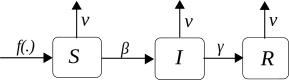
\includegraphics[width=0.6\linewidth]{SIR.pdf}
	  \caption[Diagramme du modèle SIR]{Diagramme du modèle SIR. Les compartiments représentent les individus sains ($S 
	  $), infectés ($I$) et retirés ($R$). $\beta I$ correspond à la force d'infection qui fait passer de $S$ à $I$ et 
	  $f(.)$ le flux des naissances entrant en $S$. Le paramètre $\beta$ désigne le taux de transmission, $\gamma$ le 
	  taux de guérison et $\nu$ le taux de mortalité naturelle.}
	  \label{fig:SIR}
	\end{figure}
	
Nous pouvons écrire ce modèle sous forme d'un système d'équations différentielles ordinaires :
	\begin{equation}
	  \left\{
	    \begin{aligned}
	      \frac{dS}{dt} &= f(.) - \beta SI- \nu S,\\
	      \frac{dI}{dt} &= \beta SI - \gamma I - \nu  I, \\         
	      \frac{dR}{dt} &= \gamma I - \nu R.  
	    \end{aligned}
	  \right.
	  \label{eq:SIR}
	\end{equation}
	
	Les variables d'état $S$, $I$ et $R$ dépendent du temps $t$. 
Connaissant les conditions initiales $S(0), I(0), R(0)$ à $t=0$, on peut déduire de ces équations l'évolution du système au cours du temps.
	
	Les hypothèses du modèle sont les  suivantes, en ce qui concerne les \textbf{paramètres démographiques} : 
\begin{enumerate}[label=\roman*.]
\item  $f(.)$ est une fonction qui représente les naissances par unité de temps. $f$ est positive et c'est généralement une fonction croissante de la population totale $N=S+I+R$. On suppose dans ce modèle que les individus naissent sains, donc $f$ est une entrée du compartiment $S$.
\item $\nu$ est le taux  de mortalité \og naturelle \fg{}, \textit{i.e.} indépendant de la maladie.
\end{enumerate}
et en ce qui concerne les \textbf{paramètres épidémiologiques} :
\begin{enumerate}[label=\roman*.,resume]
\item On suppose que la population est répartie de manière homogène et que la transmission est densité-dépendante, \textit{i.e.} qu'elle suit la loi d’action de masse $\beta S I$, où $\beta$ est le taux de transmission de la maladie. $\beta I$ représente la force d'infection ; d'autres formes sont présentées dans l'encadré~\ref{infection}, page~\pageref{infection}.
\item On suppose que les individus infectés sont immédiatement infectieux.
\item Les individus infectés guérissent et sont immunisés à un taux $\gamma$. 
\item Il n'y pas de surmortalité (ou agressivité) due à la maladie. Pour l'introduire, il faudrait un ajouter un  terme $- \alpha I$ à la deuxième équation du système~\eqref{eq:SIR} (qui représente l'évolution des individus $I$),
 avec $\alpha$  le taux de mortalité due à la maladie.
\end{enumerate}
	
	
	Le modèle SIR présenté en~\eqref{eq:SIR} peut se décliner de plusieurs manières. On peut par exemple considérer un modèle \textbf{en population constante}, où les naissances compensent les morts ($f=\nu N$) :
	\begin{equation}
	   \left\{
	     \begin{aligned}
	       \frac{dS}{dt} &= \nu (N - S) - \beta SI,\\
	       \frac{dI}{dt} &= \beta SI - (\gamma +\nu) I, \\         
	       \frac{dR}{dt} &= \gamma I- \nu R, 
	     \end{aligned}
	   \right.
	   \label{eq:SIR-Ncst}
	\end{equation}
	
	ou encore un modèle \textbf{sans démographie}, dans lequel il n'y a ni naissances ($f=0$) ni morts ($v=0$) : 
	\begin{equation}
		\left\{
		\begin{aligned}
			\frac{dS}{dt} &=-\beta SI,\\
			\frac{dI}{dt} &= \beta SI - \gamma I, \\         
			\frac{dR}{dt} &= \gamma I.
		\end{aligned}
		\right.
		\label{eq:SIR-nodemo}
	\end{equation}
	
	De nombreuses autres variantes du modèle SIR existent.  Par exemple, le modèle SIS permet de décrire une maladie sans immunité suite à une infection, dans lequel les individus rétablis sont susceptibles d'être réinfectés.  La possibilité intermédiaire d'une immunité temporaire peut être décrite par un modèle de type SIRS, dans lequel les individus guéris $R$ redeviennent susceptibles $S$ au bout d'un certain temps, suite à la perte de leur immunité \citep{Brauer2012}.
	
\begin{encadre2}{Force d'infection}
\label{infection}
La force d'infection $g(I,N)$ est le taux auquel un individu susceptible $S$ devient infecté. En supposant que les individus des différents compartiments sont répartis de manière homogène dans la population, on  peut décomposer la force d'infection comme suit :
	  \begin{equation*}
	    g(I,N) = c(N) \: \frac{I}{N} \: e,
	  \end{equation*}
où $c(N)$ représente le nombre de contacts par unité de temps et par individu, $\frac{I}{N}$ la probabilité que le contact ait lieu avec un individu $I$ et $e$ l'efficacité ou l'infectiosité d'un contact avec un individu $I$ (supposée constante). $c(N)$ prend généralement deux formes distinctes :
	  \begin{itemize}
\item Soit $c(N)= c_0 N$, \textit{i.e.} le taux de contact est proportionnel à la taille ou la densité de la population. On parle alors de \textbf{transmission densité-dépendante} ou de loi d'action de masse :
	    \begin{equation*}
	      g(I,N) = g(I) = c_0 e I.
	    \end{equation*}
C'est le cas du modèle SIR présenté en~\eqref{eq:SIR}, avec $\beta=c_0 e$ comme taux de transmission.
\item Soit $c(N)= c_1$, \textit{i.e.} le taux de contact est constant. On parle alors de \textbf{transmission fréquence-dépendante} :
	    \begin{equation*}
	      g(I,N) = c_1 e \frac{I}{N}.
	    \end{equation*}
 Le taux de transmission $\beta'=c_1 e$ n'est pas le même que le taux $\beta$ du cas précédent (grandeurs et unités différentes). 
 \end{itemize}
{\small \textsc{Remarque --} Dans le cas où la taille ou la densité $N$ de la population est constante, comme par exemple dans les deux variantes du modèle SIR \eqref{eq:SIR-Ncst} et \eqref{eq:SIR-nodemo}, les transmissions densité-dépendante et fréquence-dépendante sont équivalentes, avec $\beta=\beta'/N$.}
\par\medskip
	  La transmission densité-dépendante est très largement employée dans les modèles épidémiologiques, l'hypothèse que le taux de contact augmente linéairement avec la densité de population étant assez réaliste. Cependant, quand la densité de population devient très élevée, cette hypothèse est moins fondée. La transmission fréquence-dépendante est elle généralement choisie pour les maladies sexuellement transmissibles, le nombre de partenaires étant supposé indépendant de la taille ou densité de population.  Outre ces deux formes classiques pour la force d'infection, il existe d'autres modèles de transmission, qui sont par exemple présentés dans \citet{McCallum2001}.  
	\end{encadre2}
	
	
\subsubsection{Équilibres et taux de reproduction de base}
\label{sec:R0}
	Les équilibres du système (\ref{eq:SIR}) dépendent de la forme de la fonction de naissance~$f$. Le premier équilibre est $\mathcal{E}^*=(S^*,0,0)$, où $S^*$ vérifie $f(\mathcal{E}^*) = \nu S^*$.
\begin{itemize}
\item Si cette équation n'est vérifiée que pour $S^*=0$, par exemple quand $f$ est une fonction linéaire de la (densité) de population totale $f=kN$ (avec $k\neq\nu$), le premier équilibre est l'\textbf{équilibre trivial} $(0,0,0)$.
\item Si cette équation est vérifiée pour $S^*>0$, par exemple quand $f$ est une fonction constante $f=k$, alors cet équilibre $(S^*,0,0)$ est appelé \textbf{équilibre sans maladie} (\og disease free equilibrium \fg{} ou DFE en anglais), car il caractérise une situation où la maladie est absente de la population.
\end{itemize}
	
	Le second équilibre  $\bar{\mathcal{E}}=(\bar{S},\bar{I},\bar{R})$ est  appelé \textbf{équilibre  endémique}. Cet équilibre correspond à une situation où la maladie persiste dans la population et est donné par le système suivant :  
	\begin{equation}
	\left\{
		\begin{aligned}
		\bar{S} &= \frac{\nu+\gamma}{\beta}, \\
		\bar{I} &= \frac{f(\bar{S},\bar{I})}{\nu+\gamma}-\frac{\nu}{\beta},  \\
		\bar{R} &= \frac{\gamma\bar{I}}{\nu}. \\
		\end{aligned}
		\right.
	\label{sys1}
	\end{equation}
Cet équilibre n'existe que si $\bar{I}>0$, ce qui dépend de la fonction $f$ et des valeurs des paramètres.
	
	On suppose qu'il existe bien un équilibre sans maladie $\mathcal{E}^*=(S^*,0,0)$ tel que $S^*=\frac{f(\mathcal{E}^*)}{\nu}>0$. On peut alors définir le \textbf{taux de reproduction de base} du modèle SIR~\eqref{eq:SIR} comme suit :
	\begin{equation}
	  \mathscr{R}_0=\frac{\beta S^*}{v+\gamma}.
	  \label{R0}
	\end{equation}
	
	Le taux de reproduction de base est un concept clé en épidémiologie. Dans une population composée d’individus sains ($N=S^*$) dans laquelle on introduit un individu infecté, $\mathscr{R}_0$ correspond au nombre de cas secondaires d'infection engendrés par cet individu ($\beta S^*$) au cours de sa période infectieuse ($\frac{1}{\gamma + v}$) \citep{Dieckmann2000,vandenDriessche2002}. Si  $\mathscr{R}_0<1$ la maladie ne peut pas se propager, si $\mathscr{R}_0>1$ il peut y avoir une épidémie.
	
	Au niveau mathématique, $\mathscr{R}_0$ est lié à la stabilité locale de l'équilibre sans maladie : si $\mathscr{R}_0<1$ l'équilibre est asymptotiquement stable, si $\mathscr{R}_0>1$ il est instable.
En général ce seuil est lié à l'existence de l'équilibre endémique. Dans le cas, par exemple, du modèle SIR~\eqref{eq:SIR} avec naissances constantes $f=k$ :
\begin{itemize}
	\item si $\mathscr{R}_0<1$, on a un unique équilibre stable sans
	  maladie et la maladie ne peut pas s'installer ; 
	\item si $\mathscr{R}_0>1$ l'équilibre sans maladie est instable, l'équilibre endémique existe et il peut y avoir persistance de la maladie.
	\end{itemize}
	
\begin{encadre2}{Le taux de reproduction de base $\mathscr{R}_0$}
\label{encadre:R0}
 À l’origine,  $\mathscr{R}_0$ provient de la démographie \citep{Heesterbeek2002}. C’est en 1886 qu’il est introduit pour la première fois par Richard Böckh  alors qu’il cherchait à exprimer le nombre moyen de filles qu’une femme va engendrer au cours de sa vie \citep{Bockh1886}.
 \citet{Dublin1925}  définissent le $\mathscr{R}_0$ ainsi :
	  \begin{equation*}
	    \mathscr{R}_0= \int_{0}^{\infty} F(a)\beta(a) da,
	  \end{equation*}
 avec $F(a)$ la probabilité pour une femme de survivre à l’âge $a$ et $\beta(a)$ le taux de naissance de filles.
\par
Si la notion de densité seuil est apparue relativement tôt en épidémiologie, dans les travaux de \citet{Ross1911} sur le paludisme et de \citet{Kermack1927} pour les maladies à transmission directe, elle n’était au départ pas liée au $\mathscr{R}_0$. Le concept du taux de reproduction de base n’est introduit que bien plus tard  par \citet{Macdonald1952} lors de ses recherches sur le paludisme.
\par
Le concept est ensuite repris indépendamment par \citet{Dietz1975}  et \citet{Hethcote1975} pour les maladies à transmission directe. Enfin, il prend son essor dans les années 1990 grâce aux travaux méthodologiques de \citet{Diekmann1990} et au livre de référence en épidémiologie de \citet{Anderson1991}, qui lui accordent une large part.
\end{encadre2}
	
	
\subsection{Extensions du modèle SIR}
\label{sec:ext}
	 
	Le  succès du modèle SIR introduit par \citet{Kermack1932} est qu'il peut prédire le comportement de nombreuses maladies \citep{Brauer2012}. D'ailleurs, bien que les modèles compartimentaux aient été développés tout d'abord pour la compréhension et le contrôle  des épidémies  humaines puis animales, ils sont  de plus en plus appliqués en épidémiologie végétale \citep{Vanderplank1963, Madden2007,Gilligan2008}. %Van der Plank, est l'un des pionniers dans l'élaboration d'un cadre de modélisation pour l'étude de maladies transmissibles aux  végétaux (VanderPlank1960, VanderPlank1963). 
	En épidémiologie végétale les plantes sont pratiquement immobiles, mais la propagation des maladies est possible grâce à la dissémination des agents pathogènes par le vent, par l’eau ou par un vecteur \citep{Madden2007}. De nombreux modèles en épidémiologie végétale sont basés sur le modèle SIR présenté ci-dessus en section~\ref{sec:SIR}. Dans ce cadre, les variables d'état ($S,I,R$) désignent un nombre, une biomasse ou une densité de plantes, de racines, de fruits, \textit{etc.} Nous allons à présent décrire quatre extensions  possibles du modèle SIR, qui sont pertinentes en épidémiologie végétale et plus particulièrement avec notre approche de modélisation.
	
	%Les premières publications concernant les concepts associés aux modèles appliqués aux pathogènes télluriques sont dans les articles pionniers de Dimond \& Horsfall (37) et Baker (3). Par la suite, 
	%des  auteurs comme Gilligan  ont apporté une grande contribution dans le domaine de la modélisation des pathogènes télluriques \citep{Gilligan1983, Gilligan1985 Gilligan1990, Gilligan1995, Gilligan1994, Perry1983}. Toutefois, contrairement  à la  modélisation abondante des pathogènes transmis par voie aérienne \citep{Waggoner1977, thrall2002, Brown2002, Mundt2002}, la modélisation des pathogènes transmis par le sol est encore trop rare dans le  domaine de l'épidémiologie végétale \citep{Gilligan
	%1995, Thrall2007, Otten2003}.
	
\begin{quote}
	  \textsc{Notations} -- En épidémiologie humaine ou animale, le compartiment $S$ des modèle SIR désigne des individus sensibles (\og Susceptible \fg{} en anglais). En santé des plantes, le terme sensible est souvent utilisé pour désigner un trait génétique de la plante (voir~\ref{terminologie} page~\pageref{terminologie}). C'est pourquoi nous utilisons ci-dessous la notation $H$ pour les plantes saines (\og Healthy \fg{} en anglais). Par souci de cohérence avec notre modèle présenté en section~\ref{sec:notre-strategie}, nous conservons la notation classique $E$ pour les hôtes infectés en période de latence, introduite en section~\ref{sec:latence}, mais nous utilisons la notation $P$ pour la forme libre du pathogène, introduite en section~\ref{sec:libres}.
	\end{quote}

\subsubsection{La période de latence}
\label{sec:latence}
	
	Quand un individu est attaqué par un agent pathogène, il y a une période de latence durant laquelle l’agent pathogène se développe, mais l’individu hôte n’est pas encore infectieux \citep{Madden2007}. Il peut être pertinent de l'inclure dans un modèle épidémiologique, car cette période  est parfois  plus longue que la période d'infectiosité  \citep{Vanderplank1963}. Ainsi, le modèle SIR de la section précédente~\ref{sec:SIR} peut être étendu pour inclure la période de latence \citep[par exemple]{Dieckmann2000}. En épidémiologie humaine ou animale, on parle d'individus exposés (\og Exposed \fg{} en anglais) à l'infection, d'où la notation  $E$ pour le stade latent, que nous reprenons ici.
	
	À titre d'exemple, nous présentons un modèle HEIR sans démographie, où la population est mesurée en densité de racines (\autoref{fig:HEIR}). 
	
	\begin{figure}[ht]
	  \centering
		  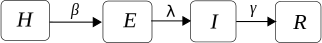
\includegraphics[width=0.6\linewidth]{HEIR}
		  \caption[Diagramme du modèle du modèle HEIR sans démographie]{Diagramme du du modèle HEIR sans démographie.  
		  Les compartiments  représentent les densités  de  racines saines ($H$), latentes  ($E$), infectées ($I$) et 
		  retirées  ($R$).
		  Le paramètre $\beta$ désigne le taux de transmission, $1/\lambda$  la durée de la période de latence et $1/
		  \gamma$ la durée de la période infectieuse.}
		  \label{fig:HEIR}
	\end{figure}
	
	En s'appuyant sur le modèle~\eqref{eq:SIR-nodemo}, nous pouvons donc écrire ce modèle HEIR selon le système d'équations différentielles suivant :
	\begin{equation}
	  \left\{
	    \begin{aligned}
	      \frac{dH}{dt} &= -\beta H I,\\
	      \frac{dE}{dt} &= \beta H I  - \lambda E, \\         
	      \frac{dI}{dt} &= \lambda E -  \gamma  I, \\
	      \frac{dR}{dt} &= \gamma I.  
	    \end{aligned}
	  \right.
	  \label{eq:HEIR}
	\end{equation}
	La différence avec le modèle~\eqref{eq:SIR-nodemo} est qu'après l'infection (flux $\beta H I$), l'agent pathogène se développe  pendant un temps $1/\lambda$ dans les racines infectées de manière latente $E$, avant que ces racines ne deviennent infectieuses $I$.
	
	

\subsubsection{La forme libre de l'agent pathogène}  
\label{sec:libres}
	
	De nombreux parasites telluriques ou aériens des plantes (bactéries, champignons, virus ou nématodes) présentent un cycle biologique complexe, où la transmission se fait via un stade de développement en dehors de la plante hôte \citep{Dwyer1994, Godfray1997}. En effet, les parasites doivent faire face à l’immobilité des plantes et donc développer des stratégies pour transmettre l’infection. Cela peut se faire par la production et dispersion massive de spores chez les champignons \citep{Agrios2005}, via un insecte vecteur pour les virus \citep{Madden2000}, ou encore grâce à une forme libre dans le sol pour les nématodes racinaires \citep{Nilusmas2017}.
Les formes libres sont souvent des formes de survie permettant au parasite non seulement de se disperser, mais aussi de survivre en l'absence d'hôtes. Chez les nématodes à kystes, les œufs peuvent rester dans le sol sous forme de kystes pendant des mois, la libération des larves dans le sol n'intervenant qu'en présence de certains exsudats de la plante \citep{Perry2018}.
	
	
	Nous présentons à titre d'exemple le modèle proposé par \citet{Cunniffe2011}, qui décrit la dynamique d'infection d'une plante par un champignon tellurique, avec un inoculum primaire sous forme libre dans le sol. Cet inoculum ($P$) correspond à des spores, des sclérotes ou encore des débris de racines précédemment colonisées. Les racines sont scindées en racines saines ($H$) et infectées ($I$). Le modèle intègre la dynamique de l'inoculum, la croissance de l'hôte et les processus d'infection des racines. Il correspond au système suivant :
	\begin{equation}
	  \left\{
	    \begin{aligned}
	      \frac{dP}{dt} &= \nu I -  \gamma P, \\
	      \frac{dH}{dt} &= \eta  \big(\kappa - (H + I)  \big) -  \big(\beta_p P + \beta_s I  \big)H,\\
	      \frac{dI}{dt} &= \big(\beta_p P +  \beta_s I  \big) H - \mu I.\\
	    \end{aligned}
	  \right.
	  \label{eq:PHI}
	\end{equation}
	L'inoculum dans le sol perd son infectiosité à un taux $\gamma$ et est reconstitué par les racines infectées à un taux $\nu$. La croissance du tissu racinaire est \og affine \fg{}, avec un taux constant $\eta\kappa$ pour les petites densités de racines (saines et infectées), qui diminue quand les racines s'approchent de leur capacité de charge $\kappa$. Il y a deux sources d'infection pour les racines saines $S$ : l'inoculum $P$ qui génère les infections primaires associées au taux de transmission $\beta_p$ ; et les racines infectées $I$, qui génèrent les infections secondaires associées au taux de transmission $\beta_s$. Dans les deux cas la transmission est supposée densité-dépendante, tout comme dans le modèle SIR~\eqref{eq:SIR} présenté en début de chapitre. Enfin, le champignon induit une mortalité des racines infectées à un taux constant $\mu$. 
	Dans ce même article, le modèle~\eqref{eq:PHI} est étendu pour prendre en compte un pathogène antagoniste aux champignons telluriques, utilisé comme agent de lutte biologique.
	
	L'existence d'une forme libre est particulièrement importante pour les agents pathogènes des agro-écosystèmes saisonniers, comme cela est décrit dans la section suivante.
	
	
\subsubsection{La saisonnalité}
\label{sec:sais}
	
	Les agro-écosystèmes saisonniers sont marqués par l'absence périodique de l'hôte, due à la récolte. 
Cette période d'absence exerce de forts goulots d’étranglement démographiques sur les populations d'agents pathogènes. Pour survivre, les agents pathogènes se tournent vers des hôtes alternatifs ou développent des stades sous forme libre (voir section~\ref{sec:libres} ci-dessus) leur permettant de supporter de longues périodes sans hôte. 
	
	Dans un système saisonnier, l'infection est initiée par un inoculum primaire, provenant d'une forme libre du pathogène, de pathogènes hébergés par des plantes sauvages ou de débris de plantes de la saison précédente. Cette infection primaire est suivie d'infections secondaires, \textit{i.e.} des infections de plante à plante \citep{Campbell1990}. Lorsque plusieurs cycles d’infections secondaires se succèdent au cours d’une saison, on parle de maladie polycyclique. À l'inverse, si la maladie repose principalement sur les infections primaires et qu'il n’y a qu’un seul cycle d’infection à partir d'une forme libre de survie, la maladie est dite monocyclique.
À la fin de la saison de culture, l'agent pathogène adopte une stratégie de survie pour affronter l’absence de l’hôte jusqu'à la saison suivante. 
	 
	La saisonnalité est modélisée par des forçages périodiques continus \citep{Murray2013} ou via des modèles semi-discrets, qui permettent d'introduire des événements discrets dans une dynamique continue. Ces modèles sont particulièrement adaptés aux agro-écosystèmes saisonniers : la partie continue représente la dynamique des interactions plante-pathogène pendant la saison de culture ; la partie discrète correspond à l'intersaison et aux changements abrupts qui affectent les populations au moment de la récolte et de la plantation. Le formalisme semi-discret est illustré sur la \autoref{fig:semi-discret}
	
	 \begin{figure}[ht]
	  \centering
		  \includegraphics[width=.9\linewidth]{semi-discrete.png}
		  \caption[Illustration du formalisme semi-discret.]{Illustration du formalisme  semi-discret.
		    Le trait plein de l’axe du temps représente les phénomènes continus pour $t \in (\tau_k;\tau_{k+1})$  
		    (\textit{e.g.} cycles d’infection, croissance de l'hôte). Le trait discontinu représente les phénomènes 
		    discrets pour $t = \tau_k$ ($e.g$  récolte et plantation de l'hôte, survie du parasite sous forme libre).
		    D'après \citet{Mailleret2009}.}
		  \label{fig:semi-discret}
	 \end{figure}
	
	\citet{Shaw1994} est le premier à avoir utilisé un modèle semi-discret pour décrire la dynamique d'une épidémie végétale. Il a montré qu'un tel modèle peut conduire à des dynamiques chaotiques, tandis que sans discontinuités, les modèles convergent vers des équilibres stables. Par la suite, des modèles semi-discrets ont été utilisés dans des agro-écosystèmes saisonniers pour étudier la persistance d'agents pathogènes \citep{Madden2002}, l'évolution et la coexistence de pathogènes \citep{Vandenberg2010,Vandenberg2011,Hamelin2011,Mailleret2012}, ou encore pour déterminer des stratégies de déploiement de plantes résistantes \citep{Fabre2012,Fabre2015}. Nous en présentons deux ci-dessous : le modèle de  \citet{Vandenberg2011} et celui de \citet{Mailleret2012}.
	
	%\citet{Madden2002} : modèle  type SEIR avec saisonnalité ; conditions nécessaires à la persistance à long terme d'une maladie végétale après l'introduction d'un micro-organisme pathogène dans une culture annuelle sensible .
	
	
	Le modèle de \citet{Vandenberg2011} est fondé sur un modèle épidémiologique classique décrivant l'évolution des densités d'hôtes sains ($H$) ou infectés ($I$) pendant la saison de culture, auquel on introduit une forme libre de survie du pathogène ($P$) présente uniquement pendant l'intersaison. Il intègre également la croissance de la plante hôte. La dynamique du modèle est décrite ci-dessous et illustrée dans la \autoref{fig:vandenberg}.
	
	\begin{figure}[ht]
	  \centering
	  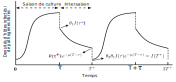
\includegraphics[width=1\linewidth]{vandenberg_sais.pdf}
	  \caption[Dynamique du modèle épidémiologique semi-discret de \citet{Vandenberg2011}]{Dynamique du modèle 
	  épidémiologique semi-discret de \citet{Vandenberg2011}, décrit dans les équations (\ref{eq:vandenberg-saison}-
	  \ref{eq:vandenberg-plant}). L'évolution de l'épidémie est représentée en suivant : la densité d'hôtes infectés 
	  ($I$) pendant les saisons de cultures, \textit{i.e.} pour $t\in(nT^+,nT+\tau^-)$, avec $n=0,1$ ; et la densité de 
	  pathogènes sous forme libre ($P$) pendant l'intersaison, \textit{i.e.} pour $t\in(nT+\tau^+,(n+1)T^-)$. Les sauts 
	  représentent les récoltes ($nT+\tau$) ou les plantations ($nT$) avec $P(\tau^+)=\theta_1 I(\tau^-)$, 
	  $P(T^-)=P(\tau^+)e^{_\mu(T-\tau)}$, $I(T^+)=\theta_2P(T^-)$. 
	   Adapté de \citet{Vandenberg2011}.}
	  \label{fig:vandenberg}
	\end{figure}
	
	On considère la saison $n$, avec $n=0,1,\ldots$
\begin{enumerate}
\item \emph{Saison de culture, soit $t\in(nT^+,nT+\tau^-)$}\quad
Le pathogène sous forme libre est absent, la croissance, la mortalité et l'infection de la plante hôte sont représentées : 
	\begin{equation}
	  \left\{
	    \begin{aligned}
	      P~ &= 0, \\
	      \frac{dH}{dt} &=  f(H,I) - \beta HI - \nu H,   \\
	      \frac{dI}{dt} &= \beta HI - (\nu+\alpha) I,
	    \end{aligned}
	  \right.
	  \label{eq:vandenberg-saison}
	\end{equation}
	avec $f(H,I)$ la fonction de croissance des hôtes, $\beta$ le taux de transmission supposée densité-dépendante, $\nu$ le taux de mortalité naturelle des hôtes et $\alpha$ l'agressivité, \textit{i.e} la mortalité induite par le pathogène.
	\item  \emph{Récolte, soit $t=nT+\tau$}\quad
	  À la fin de chaque saison de culture, les plantes sont arrachées et le pathogène se tourne vers une stratégie de survie ($P$):
	  \begin{equation}
	    \left\{
	      \begin{aligned}
	        P(nT+ \tau^{+}) &= \theta_1 I(nT+\tau^{-}),\\
	        H(nT+ \tau^{+}) &=0,   \\
	        I(nT+ \tau^{+}) &=0,
	      \end{aligned}
	    \right.
	    \label{eq:vandenberg-recolte}
	  \end{equation}
	  avec $\theta_1\in(0,1)$ la proportion d'hôtes infectés ($I$) qui alimentent la forme libre du pathogène ($P$). 
	\item  \emph{Intersaison, soit $t\in(nT+\tau^+,(n+1)T^-)$}\quad
	  L'hôte est absent et le pathogène sous forme libre  meurt à un taux $\mu$ :
	  \begin{equation}
	    \left\{
	      \begin{aligned}
	        \frac{dP}{dt} & = -\mu P, \\
	        H &= 0, \\
	        I~ &= 0. \\
	        \end{aligned}
	    \right.
	    \label{eq:vandenberg-intersaison}
	\end{equation} 
	\item  \emph{Nouvelle saison, soit $t=(n+1)T$}\quad
	  Au début de la saison de culture suivante, une proportion $\theta_2 \in (0,1)$ des pathogènes sous forme libre retournent dans l'hôte et initient la phase épidémique :
	  \begin{equation}
	   \left\{
	      \begin{aligned}
	        P((n+1)T^{+}) &= 0,\\
	        H((n+1)T^{+}) &=H_0 - I((n+1)T^{+}),   \\
	        I((n+1)T^{+}) &=\theta_2 P((n + 1)T^-),
	      \end{aligned}
	    \right.
	    \label{eq:vandenberg-plant}
	  \end{equation}
	  où  $H_0$ est la densité de culture au début de chaque saison, supposée constante.
	\end{enumerate}	
	
	Les auteurs ont étudié l'influence de deux compromis : l’un entre transmission ($\beta$) et agressivité ($\alpha$) et l'autre entre transmission et survie du pathogène sous forme libre ($\mu$). Notamment, ils ont montré  que des durées d'intersaison plus longues sélectionnent des taux de transmission $\beta$ plus élevés dans le cas du compromis $\beta$--$\alpha$, mais plus faibles dans le cas du compromis $\beta$--$\mu$. En l’occurrence ils ont démontré que dans ce système, l’évolution tend a maximiser le $\mathscr{R}_0$ du pathogène.
Dans un environnement périodique,  $\mathscr{R}_0$ est obtenu en linéarisant le système au voisinage de l'état stationnaire sans maladie \citep{Bacaer2006, Bacaer2007}.

	%\citet{Vandenberg2010} par différents  modèles en temps continu
	%avec des dynamiques d’infections dite aérienne ou tellurique combiné avec des épisodes discrets, ont étudié dans quelle mesure l'absence périodique d'hôte  engendre un branchement évolutif. En se basant sur des simulations numériques, 
	%les auteurs ont conclu que \og la périodicité de la disponibilité des hôtes
	%ne permet pas de générer un branchement évolutif, comme observée chez de nombreux agents pathogènes des plantes \fg{}.  
	
	Le second modèle présenté est celui de \citet{Mailleret2012}, basé sur le modèle de \citet{Madden2002}. Il décrit la dynamique épidémique saisonnière d'un pathogène de plante aérien ou tellurique, avec infections primaires et secondaires. La seule différence entre les deux versions du modèle est la forme du taux de dégradation de l'inoculum primaire (forme de survie du pathogène) pendant la saison de culture : il dépend de la densité d'hôtes pour le pathogène tellurique (propagules relâchées suite à un signal chimique de la plante), mais pas pour le pathogène aérien (spores relâchées selon les conditions environnementales). Il est représenté sur la \autoref{fig:mailleret} et sa dynamique est décrite ci-dessous.
	
	\begin{figure}[ht]
	  \centering
	   \includegraphics[width=1\linewidth]{Mailleret_semi-discrete}
		\caption[Diagramme du modèle épidémiologique semi-discret de \citet{Mailleret2012}]{Diagramme du modèle  
	    épidémiologique semi-discret de \citet{Mailleret2012}, correspondant aux équations~(\ref{eq:mailleret-saison}--
	    \ref{eq:mailleret-plant}). Deux périodes se succèdent pendant l'année de durée $T$ : 
	    la saison de culture, durant  laquelle la plante hôte est présente ($t \in (nT, nT + \tau])$ ; 
	    et la saison hivernale sans plante hôte $(t \in 
	    (nT + \tau, (n + 1)T])$. Le compartiment $P$ représente l'inoculum primaire (forme libre du pathogène), $H$ les 
	    plantes saines et $I$ les plantes infectées.
	    Les flèches pleines représentent les processus continus : infections primaires (taux $\Theta$) et secondaires 
	    (taux $\beta$), ainsi que mortalité liée à l’infection (taux $\alpha$) pendant la saison de culture ; mortalité 
	    de l'inoculum primaire (taux $\mu$) pendant la saison hivernale. Les flèches en pointillés représentent les 
	    processus discrets : plantation d’une nouvelle culture ($H_0$) au début de la saison de culture ; arrachage des 
	    plantes (ou perte des feuilles) et conversion des plantes infectées en inoculum primaire (taux $\pi$) au début 
	    de la saison hivernale. Adapté de \citet{Mailleret2012}. }
		\label{fig:mailleret}
	\end{figure}
	
	On considère, comme précédemment, la saison $n$, avec $n=0,1,\ldots$
\begin{enumerate}
\item \emph{Saison de culture, soit $t\in(nT^+,nT+\tau^-)$}\quad
La dégradation de l'inoculum primaire ($P$) pour un pathogène aérien (taux $\Lambda$) ou tellurique (taux densité-dépendant $\Xi$), les infections primaires (taux $\Theta$) et secondaires (taux $\beta$) des plantes saines ($H$), supposées densité-dépendantes, ainsi que  la mortalité (taux $\alpha$) des  plantes infectées ($I$) sont représentées : 
	\begin{equation}
	  \left\{
	    \begin{aligned}
	      \dot{P} &=
	      \left|
	      \begin{aligned}
	        &- \Lambda P &&\text{pathogène aérien} \\
	        &- \Xi P H &&\text{pathogène tellurique}
	      \end{aligned}
	      \right.\\
	      \dot{H} &= - (\Theta P  + \beta I) H,\\
	      \dot{I} &= + (\Theta P  + \beta I) H - \alpha I.
	    \end{aligned}
	  \right.
	  \label{eq:mailleret-saison}
	\end{equation}
	\item  \emph{Récolte, soit $t=nT+\tau$}\quad
	  À la fin de chaque saison de culture, les plantes sont arrachées (les feuilles des arbres tombent) et les débris de plantes infectées sont convertis en inoculum primaire (taux $\pi$) :
	  \begin{equation}
	    \left\{
	      \begin{aligned}
	        P(nT+ \tau^{+}) &= P(nT + \tau) + \pi I(nT + \tau),\\
	        H(nT+ \tau^{+}) &=0,   \\
	        I(nT+ \tau^{+}) &=0.
	      \end{aligned}
	    \right.
	    \label{eq:mailleret-recolte}
	  \end{equation} 
	\item  \emph{Saison hivernale, soit $t\in(nT+\tau^+,(n+1)T^-)$}\quad
	  L'hôte est absent et l'inoculum primaire se dégrade (taux $\mu$) :
	  \begin{equation}
	    \left\{
	      \begin{aligned}
	        \frac{dP}{dt} & = -\mu P, \\
	        H &= 0, \\
	        I~ &= 0. \\
	        \end{aligned}
	    \right.
	    \label{eq:mailleret-intersaison}
	\end{equation} 
	\item  \emph{Nouvelle saison, soit $t=(n+1)T$}\quad
	  Au début de la saison de culture suivante, de nouveaux hôtes sains sont plantés (les feuilles des arbres apparaissent) :
	  \begin{equation}
	   \left\{
	      \begin{aligned}
	        P((n+1)T^{+}) &= 0,\\
	        H((n+1)T^{+}) &= H_0, \\
	        I((n+1)T^{+}) &= 0.
	      \end{aligned}
	    \right.
	    \label{eq:mailleret-plant}
	  \end{equation}
	\end{enumerate}
		
	En supposant que les infections primaires sont rapides par rapport aux autres processus, les auteurs ont obtenu et étudié des modèles réduits \og compacts \fg{}, pour les pathogènes aérien et tellurique. Par ailleurs, ils se sont intéressés à la coexistence de deux souches de pathogène, en supposant qu'une souche est plus performante pendant la saison de culture (taux d'infection secondaire $\beta$ plus élevé) et l'autre pendant la saison hivernale (taux de mortalité $\mu$ plus faible). Ils ont montré que la coexistence des deux souches est possible pour le pathogène aérien, mais pas pour le pathogène tellurique, qui ne diffère du pathogène aérien que par la forme densité-dépendante du taux de dégradation de l'inoculum primaire. Ce résultat révise les conclusions de \citet{Vandenberg2010,Vandenberg2011}, qui sont fondés sur des modèles d'évolution en environnement saisonnier dans lesquels le principe d'exclusion compétitive\footnote{Principe d'exclusion compétitive (ou principe de Gause) : deux populations partageant la même niche écologique (\textit{e.g.} exploitant une ressource limitante unique) ne peuvent coexister indéfiniment.} s'applique.
	
	
\subsubsection{Hôtes résistants et  pathogènes virulents}
\label{sec:resist-virul}
	
	
	
	L'utilisation de variétés résistantes est un moyen de lutte à la fois efficace et respectueux de l'environnement (voir section \ref{sec:resistance} du chapitre \ref{intro}). Cependant, leur déploiement intensif peut mener à des contournements par des pathogènes virulents (voir section \ref{contournement} du chapitre \ref{intro}). Ainsi, différents travaux de modélisation se sont intéressés aux interactions entre plantes sensibles et résistantes, d'une part, et pathogènes avirulents et virulents, d'autre part, afin d'améliorer la durabilité des résistances ou le rendement des cultures \citep{vandenBosch2003,Fabre2012,Papaix2014,Fabre2015,Lof2017,Djidjou-Demasse2017}. 
Nous présentons ci-dessous plus en détails le modèle de \citet{Fabre2012} et son extension \citet{Djidjou-Demasse2017} qui sont aussi fondés sur un formalisme semi-discret.
	
	\citet{Fabre2012} ont recherché des stratégies de déploiement des plantes résistantes en fonction des caractéristiques du cultivar résistant, de l'aménagement du paysage et des pratiques culturales. Pour ce faire les auteurs ont développé un modèle décrivant la dynamique saisonnière d'une population de virus dans un paysage composé de culture résistantes et sensibles  dans une  mosaïque.
Pour  nombreux champignons ou nématodes phytoparasites, les virus responsables des maladies des plantes dépendent de leur hôte pour survivre et  la transmission du virus  a lieu lorsque les plantes  entrent en contact avec le virus ou via des vecteurs du virus. En cas d'absence de plantes cultivées, des réservoirs naturels (plantes sauvages, adventices) abritent le virus toute l'année, ainsi le virus peut donc survivre à l'hiver. L'infection primaire  démarre la phase épidémique. La propagation de la maladie est assurée par les infections secondaires : le virus se transmet aux plantes du même champ (auto-infection) ou  aux plantes des champs limitrophes (allo-infection).  Par conséquent, ces voies d'infection (i) entre le réservoir et les champs, (ii) entre les plantes du  même champ et (iii)  entre les plantes des autres champs peuvent éventuellement influencer les dynamiques des épidémies virales.
	
	Pour modéliser la saisonnalité des systèmes de culture, ils ont utilisé un modèle semi discret \citep{Mailleret2009}.  Ici, la partie continue est représenté par un modèle de type SI décrivant les dynamiques de transmission de l'infection de plantes à l'intérieur du même champ et  de plantes provenant d'autres champs.  Le paysage est composé de deux génotypes d'hôtes cultivés sensibles  et résistants   et deux variantes de virus avirulent  et virulent. Le cultivar sensible peut être infecté par les deux variants du virus. La plante résistante (porteuse de gènes R et impliquée dans une relation gène pour gène) peut être infectée uniquement par le variant virulent.  Le modèle permet de simuler l'épidémie d'une maladie virale pendant des années $y \in ([1,n_y])$ dans un paysage saisonnier et d'un réservoir de virus.  
		
	Nous décrivons d'abord le modèle dans un paysage composé uniquement de cultivar sensible. $\phi$ étant la proportion de champs composés de  plantes résistantes, ici $\phi = 0$.
	
	
	\begin{equation}
	\frac{I_{S,y}}{dt} = (n_p - I_{S,y})(\alpha_{E} + \beta_C (n_f -1) I_{S,y} + \beta_F I_{S,y})
	\label{sys4}
	\end{equation}
	
	
	Le compartiment $I_{S,y}$ représente  le nombre de plantes infectées dans un champ sensible donné au cours de l'année $y$. La taille de la population hôte est de $n_p$ plantes par champ. Le nombre de nouvelles infections par unité de temps est déterminé par le principe de l'action de masse entre les plantes saines et infectées, qui implique des contacts aléatoires entre les plantes.   Les épidémies virales se propagent dans une métapopulation d'hôtes composée de champs de taille $n_f$  et d'un réservoir.  Trois voies d'infection sont considérées dans ce paysage :  (i) entre le réservoir et les champs, (ii) entre les champs et (iii) à l'intérieur d'un champ. Les plantes saines $n_p - I_{S,y}$ peuvent contracter la maladie à partir des plantes  infectées $I_{S,y}$ dans le même champ à un taux de contact $\beta_F $ (unité : plante $^{-1} \cdot t^{-1}$)  ou à partir des plantes infectées dans les autres champs $(n_f -1) I_{S,y}$  à un taux de contact $\beta_C$ ( plante$^{-1} \cdot t^{-1}$).  Les plantes saines peuvent également contracter la maladie à partir de plantes infectées dans le compartiment du réservoir à un taux $\alpha_E$ (t$^{-1}$). La taille du réservoir n'est pas explicitement modélisée.
	
	Le modèle est étendu pour prendre en compte la proportion $\phi$ de champs cultivés composés de plantes résistantes : 
	\begin{align}
	\frac{I_{S,y}}{dt} &= (n_p - I_{S,y})\big[\alpha_{S,y} + \beta_C \big[((1-\phi)n_f -1) I_{S,y} + \phi n_f I_{R,y}\big] + \beta_F I_{S,y}\big] \label{sys5} \\ 
	\frac{I_{R,y}}{dt} &= (n_p - I_{R,y})\big[\alpha_{R,y} + \beta_C \big[(1-\phi)n_f \theta I_{S,y}) + (\phi n_f -1) I_{R,y} \big] + \beta_F I_{R,y}\big] \label{sys7} 
	\end{align}
	
	 Les équations \eqref{sys5} et \eqref{sys7}  permettent de prendre en compte les infections depuis les champs résistants vers les champs sensibles  et inversement. On sait que dans un champ composé de plantes résistantes seuls les variants virulents sont présents, tandis que dans les champs composés de plantes sensibles les variants virulents et avirulents dit \og sauvages \fg sont présents. Dans ce cas de figure, deux génotypes sont en compétition pour les ressources de la plante sensible. Dans l'équation \eqref{sys7}, le paramètres $\theta$ représente la fréquence de variants virulents qui coexistent avec le variant sauvage  à l'équilibre dans un champ ou parcelle composé uniquement de plantes sensibles. La fréquence de variants virulents à un équilibre de \og mutation-sélection \fg va dépendre du taux de mutation pour contourner la résistance et des coûts de fitness associés à l'acquisition de la virulence. Ce paramètre est donc un paramètre important car il représente les caractéristiques du gène de résistance.   
Durant l'hiver, la fréquence des variants au sein du  réservoir dépend de leur fréquence dans le paysage.
	
	Les auteurs ont étudié à partir de leur métrique pour différents scénarios épidémiologiques l'effet du ratio de plantes résistantes et des caractéristiques de la résistance. 
Ils ont conclu qu'il n'y a pas de stratégies universellement optimales (résistance pure \textit{vs} mosaïque).
 Les auteurs ont montré que l'intensité des épidémies jouait un rôle important sur les dommages relatifs et donc sur la  gestion de l'épidémie virale.
Lorsque l'intensité des épidémies était élevée et pour toutes les résistances testées une stratégie mosaïque était optimale.
Le choix du gène majeur de résistance (\textit{i.e.} le nombre de mutations nécessaires au contournement et le coût de fitness associé à chaque mutation dans les plantes sensibles) et le ratio de plantes est un facteur important dans la stratégie de déploiement de la résistance. Un ratio plus important  de plantes résistantes pouvait être déployé lorsque le gène de résistance était associé à de très forts coûts de fitness. En outre, dans le cas où la voie principale d'infection se faisait au niveau du réservoir une stratégie 100 \% résistant pouvait être optimale, parce que le réservoir hébergeait initialement très peu de variants virulents, ce qui entraîne peu d'infections de plantes résistantes. Par contre, lorsque les infections se faisaient principalement entre champs, des proportions intermédiaires de plantes résistantes étaient optimales. Ce résultat était possible grâce à l'effet de dilution qui tend à réduire les transmission de la maladie et donc la gravité des épidémies dans les mélanges de cultivars (voir sous sous section~\ref{durabilite_sub}.\ref{subsubsec:mel}). 
Cette étude a permis de démontrer l'importance des études numériques pour fournir des recommandations quant à un déploiement efficace et durable de la résistance à un virus en fonction des différents leviers d'actions des agriculteurs. Cette étude montre l'importance que constitue une stratégie mosaïques pour le contrôle d’une
maladie virale, en fonction des facteurs tels la connectivité entre les champs et réservoir et deux autres voies d'infections, l’intensité des épidémies et les caractéristiques du gène majeur de résistance. 
	
	\citet{Djidjou-Demasse2017} ont étendu ce modèle pour pouvoir considérer plusieurs gènes de résistance. Ils ont comparé les performances des stratégies de déploiement de deux à cinq gènes de résistance dans le paysage, obtenues soit en combinant les cultivars sensible et résistants monogéniques sous forme d'une mosaïque paysagère, soit en combinant les cultivars sensible et pyramidé. Ces stratégies faisaient intervenir des proportions prédéfinies ou optimisées des différents cultivars , ces proportions étant uniformes ou variables dans le temps.
Les auteurs ont conclu que les mosaïques étaient plus efficaces que le  pyramidage pour réduire les dommages causés par les pathogènes.
	
\section{Modèles appliqués aux nématodes des racines}
\label{sec:modeles-nematodes}
	
	Il existe différents  types de modèles dans la littérature. Tout d'abord, on retrouve ceux qui modélisent les dynamiques de populations à l’échelle d'un cycle cultural, qui représentent la grande majorité des approches. Ensuite, il existe  des modèles plus spécifiques qui s'attachent plus particulièrement à une phase du cycle de vie comme par exemple les modèles de survie hivernale \citep{Jeger1985, Starr1985, Jeger1993} . Enfin, plus rarement,  des  modèles multi-saisons qui permettent de développer un cadre de modélisation pour l'étude de stratégies de contrôle des nématodes  (\textit{e.g.} rotations, jachères, utilisation de pesticides) et/ou de leur évolution sur le long terme (\textit{e.g.} leur capacité à contourner un \gls{gene R}). 
	
	
\subsection{Une saison  de culture}
\label{sec:une-saison}
	
	
\subsubsection{Modèles de perte de rendement}
\label{sec:perte-de-rendements}
	
	Différentes équations ont été proposées pour mettre en relation la densité de population initiale de nématodes $P_i$ et le rendement de la culture $Y$ ou  le rendement relatif $y=\frac{Y}{Y_{max}}$, où $Y_{max}$ est le rendement attendu en l'absence de nématodes, notamment pour les nématodes à kystes de la pomme de terre (\textit{Globodera}) ou pour les nématodes à galles (\textit{Meloidogyne}).
	
	\citet{Brown1969} a effectué des régressions linéaires entre le rendement et le nombre initial d'œufs (avec ou sans transformation logarithmique) ou de kystes (avec ou sans transformation en racine carrée). \citet{Oostenbrink1966} a également utilisé un modèle de régression linéaire avec transformation logarithmique. %\stcom{Je n'ai pas ce dernier papier, à vérifier.}
	
	\citet{Seinhorst1965} a introduit une relation empirique entre rendement relatif ($y$) et densité initiale de nématodes ($P_i$), qui s'ajuste bien à des données expérimentales. Elle  est donnée  par cette équation :  
	\begin{equation}
	    \begin{cases}
	      y  =  m + (1-m)  z^{P_i-T} & \text{si }  P_i>T,  \\
	      y  = 1 &\text{si } P_i \leqslant T,
	    \end{cases}
	  \label{eq:Seinhorst1965}
	\end{equation}
où $P_i$ est la densité de population de nématodes dans le sol
au moment des semences ou de la plantation de la culture (exprimée en
œufs et/ou J2 par cm$^3$ ou g de sol) ; $T$ est la  tolérance, soit le seuil d'infestation initiale en dessous duquel aucun dommage n'est subi par la plante ;  $m$ est le ratio entre le rendement minimal à des valeurs très élevées de densité initiale de nématodes ($Pi  \rightarrow \infty$)  et le rendement maximal $Y_max$ (des valeurs de $m$ proches de 1 peuvent correspondre à un cultivar résistant) ; $y$ est le rendement relatif (le rendement à un
	 $P_i$ donné divisé par le rendement à $P_i$  $\leq$ $T$) ; et $z$ est une constante telle que $z<1$. \citet{Seinhorst1965,Seinhorst1970} a montré que $z^{-T}$  prend en général des valeurs entre $1$ et $1,15$.
	
	Ce modèle, qui a l'avantage d'être simple, a été utilisé surtout pour modéliser des
dommages causées par  une ou plusieurs générations de nématodes sur une
saison de culture. L'auteur l'a employé dans divers travaux \citep[par exemple]{Seinhorst1965,Seinhorst1970, Seinhorst1972, Seinhorst1986, Seinhorst1998}.
Dans la littérature,  de nombreux  travaux ont utilisé ce modèle  dans le  but de reproduire assez fidèlement des données issues d'expériences sur le terrain ou en conditions contrôlées ou semi-contrôlées. Une grande partie de ces travaux sont répertoriés  dans l'article  de  \citet{Greco2010}. Cet article fournit notamment les valeurs des paramètres  ($T$, $m$ et $z$) pour une grande variété de plantes et pour les espèces très préoccupantes du genre \textit{Meloidogyne}. Certains travaux sont repris ci-dessous.
	
	 \citet{Duncan1983} ont modélisé les effets des nématodes à galles \textit{Meloidogyne javanica} et \textit{M.~incognita} sur la croissance du niébé cv.~\textit{Californian Blackeye No.~5}  et ont montré que les dommages étaient plus importants avec \textit{M.~javanica} qu'avec \textit{M.~incognita}.  \citet{McSorley1992} ont montré  que l'effet de \textit{M.~arenaria} sur le rendement de l'arachide pouvait être modélisé efficacement à l'aide de ce modèle de Seinhorst~\eqref{eq:Seinhorst1965}. 
	%\stdel{Ils ont obtenu  comme valeurs de  paramètres : $T=1$ oeuf/100cm$^3$ de sol, $m=0,088$ et $z=0,90$.}
	
	\citet{Ehwaeti1998} ont mené une étude expérimentale pour examiner les dommages causés par
\textit{M.~incognita} à des  tomates, \textit{Lycopersicon esculentum}, cv.~\textit{Moneymaker} et ils ont mis en relation la densité initiale de  nématodes dans le sol avec un proxy de rendement relatif de tomates  à 42 et 135 jours de culture (\autoref{fig:Ehwaeti1998}). Cette approximation du rendement relatif est le ratio entre la biomasse racinaire  de tomates en présence et en absence de nématodes à 42 jours et à 135 jours après inoculation. De plus, ils ont ajusté leurs données expérimentales au  modèle de Seinhorst~\eqref{eq:Seinhorst1965}.
	%\stdel{Après 135 jours de culture, soit trois générations de nématodes, ils ont obtenu  comme estimation comme valeurs de  paramètres :$T =0,032$ œuf/g de sol, $z= 0,42$ et $m= 0,23$.}
	
	\begin{figure}[htp]
		\centering \includegraphics[width=1\linewidth]{ehwaeti2000-rendement.pdf}
		\caption[Rendement relatif de tomate en fonction des densités initiales de \textit{Meloidogyne incognita} dans le sol \citep{Ehwaeti1998}.]{Relation entre les densités initiales de populations  de nématodes \textit{Meloidogyne incognita} dans le sol et la biomasse relative de tomate (\textit{i.e.} ratio entre  biomasse racinaire  en présence et en absence de nématodes) à 42 et 135 jours post inoculation. Les courbes montrent l'ajustement au modèle de Seinhorst~\eqref{eq:Seinhorst1965}. D'après \citet{Ehwaeti1998,Ehwaeti2000}.}
		\label{fig:Ehwaeti1998}
	\end{figure}
		
	\citet{DiVito2004} ont modélisé la  relation entre les densités de populations initiales de \textit{M. incognita} et la perte de rendement du haricot cultivé en pots dans une serre (\autoref{Divito}).
	
\begin{figure}[hbtp]
\centering \includegraphics[width=1\linewidth]{Di_vito.png}
\caption[Rendement relatif de haricot en fonction des densités initiales de \textit{Meloidogyne incognita} dans le sol \citep{DiVito2004}.]{Relation entre les densités de populations initiales de \textit{Meloidogyne incognita} ($P_i$) et le rendement relatif ($y$) du haricot cultivé en pots dans une serre. Les courbes montrent l'ajustement au modèle de Seinhorst~\eqref{eq:Seinhorst1965}, les valeurs des paramètres $T$ et $m$ sont indiquées. D'après \citet{DiVito2004}.}
\label{Divito}
\end{figure}
	
	D'autres modèles ont été utilisés pour représenter la perte de rendement. \citet{Elston1991} ont étudié l'impact des nématodes à kystes de la pomme de terre (\textit{Globodera pallida}) sur cinq génotypes de pomme de terre partiellement résistant et un non résistant cultivés aux champs. Ils ont introduit un modèle linéaire inverse entre rendement relatif et densité initiale de nématodes : 
	\begin{equation}
		y = 1 - \frac{(1-m) P_i}{c + P_i}
		\label{eq:Elston1991}
	\end{equation}
	où $m$ correspond au paramètre du modèle de Seinhorst~\eqref{eq:Seinhorst1965}, soit le ratio entre le rendement minimal à des valeurs élevées de densité de nématodes et le rendement maxima sans nématodes, et $c$ est une constante. Dans cette étude, ils ont conclu que ce modèle alternatif pouvait décrire la perte de rendement avec moins de paramètres que le modèle de Seinhorst. 
	De plus, ils ont constaté que lorsque le paramètre $m$ était ramené à zéro,  cela ne nuisait pas à l'ajustement du modèle aux données.  Ils ont donc  proposé un modèle  plus simple encore, correspondant au modèle \eqref{eq:Elston1991} avec $m=0$ :
	\begin{equation}
		y =\frac{1}{1 + \frac{P_i}{c}}.
		\label{eq:Elston1991si}
	\end{equation}
	
	\medskip
	La plupart des modèles  de la littérature appliqués aux nématodes sont  des équations  qui relient les  populations finales de nématodes (\ref{eq:Seinhorst1966-migratory}--\ref{eq:Jones1978}) ou le rendement (\ref{eq:Seinhorst1965}--\ref{eq:Elston1991si}) aux populations initiales de nématodes sur une saison. Le seul paramètre ayant une  interprétation biologique claire est la tolérance $T$, \textit{i.e.} la faculté de l'hôte à tolérer le pathogène durant une saison de culture. 
	
	
	\subsubsection{Modèles de la dynamique des nématodes}
	
	Ces modèles relient les densités de nématodes en début et fin de saison de culture. Ils ont été introduits par \citet{Seinhorst1966,Seinhorst1967a,Seinhorst1967b,Seinhorst1967c,Seinhorst1970} et ont ensuite été largement repris.
	
	
	Cet auteur a utilisé le modèle logistique (voir Encadré~\ref{logistique}) pour représenter la dynamique des nématodes et relier la densité de population finale $P_f$ avec la densité de population initiale $P_i$ :
	\begin{equation}
	  P_f =  \frac{E_1 P_i e^{rt}}{ E_1 - P_i + P_i e^{rt}},
	  \label{eq:Seinhorst1966-migratory}
	\end{equation}
	
	où $e^{rt}$ est le nombre de descendants viables par femelle à l'instant $t$, avec $r$ le taux d'accroissement intrinsèque, et $E_1$ est la densité de nématodes à l'équilibre, soit la capacité de charge du modèle logistique (généralement notée $K$). 
	
	Ce modèle s'applique à la dynamique d'une large gamme de nématodes parasites des plantes. Cependant, il est plus approprié aux nématodes migrateurs (\textit{e.g.} l'ectoparasite \textit{Tylenchorhynchus dubius}), qui se multiplient continuellement pendant la croissance d'une culture hôte \citep{Seinhorst1970}. 
		
	Un autre type de modèle,  basé sur le modèle de compétition de
	\citet{Nicholson1935} et sur une courbe logistique,  décrivant la relation entre la densité initiale ($P_i$) dans le sol  et la densité finale ($P_f$) à  la fin d'une saison de culture a été proposé par  \citet{Seinhorst1967c,Seinhorst1970,Seinhorst1986} :
	\begin{equation}
		% P_f= a y\frac{ (1-q^{P_i})}{-{^e{log(q)}}} = y M  (1- e^{-x})
		P_f= a y\frac{ \left(1-q^{P_i}\right)}{-\ln(q)} = y M  \left(1- e^{-a P_i M^{-1} }\right)
		\label{eq:Seinhorst1970-sedentary}
	\end{equation}
	avec M = $a {(-\ln(q)})^{-1}$.
Dans cette   équation, $q<1$ est une constante très proche de 1  et peut être considérée comme la proportion de sites  potentiels pour le nématode ;
$a$ est le taux de multiplication maximum du nématode;  
$M$ est la densité de population maximale théorique en l'absence
de dommages ; et $y$ représente le rendement relatif. Le paramètre $P_i$ est généralement connu, il faut donc estimer les paramètres $M$, $y$ et $a$ grâce à des données issues d'études expérimentales bien réalisées. L'estimation du rendement relatif $y$ est obtenue par l'ajustement de données expérimentales au modèle de Seinhorst~\eqref{eq:Seinhorst1965} car le paramètre $y$  est généralement considéré comme le même $y$ dans les deux modèles de Seinhorst~ \eqref{eq:Seinhorst1965} et~\eqref{eq:Seinhorst1970-sedentary}. 
	
	\begin{encadre2}{Modèle de Verhulst}
	  \label{logistique}
	  En 1837, le biologiste belge Pierre-François Verhulst introduit le  modèle logistique en temps continu \citep{Verhulst1838} . Ce modèle permet de reproduire les dynamiques de nombreux macro- et micro-organismes. Il prend en compte  un processus d’autorégulation de la population observée, ou encore de compétition intra-spécifique pour les ressources (nourriture ou/et territoire) \citep{Brauer2012}.
	  Dans ce modèle, la dynamique de  la population  $P$ au cours du temps $t$ est donnée par :
	  \begin{equation*}
	    \left\{
	      \begin{aligned}
	        \dot{P}(t)&= rP(t) \left(1 - \frac{P(t)}{K}\right),\\
	        P(0)&= P_0,
	      \end{aligned}
	    \right.
	  \end{equation*}
où $r$ est le taux de croissance, $K$ la capacité de charge (\og carrying capacity \fg{} en anglais)  de la population et $P_0$ la taille initiale de la population. En intégrant cette équation, on trouve :
	  \begin{equation*}
	        P(t) = \frac{KP_0e^{rt} }{ K - P_0+ P_0 e^{rt}} = \frac{K}{1+\left(\frac{K}{P_0}-1\right) e^{-rt}} \quad  
	        \forall t \geqslant 0.
	  \end{equation*}
	 	La croissance logistique correspond à une croissance quasi exponentielle pour des faibles tailles de population, avec une saturation quand cette taille approche de la capacité de charge $K$. Cette dernière représente la taille de population maximale qui peut être maintenue de manière durable à partir des ressources disponibles.  Par ailleurs, l'équation logistique possède deux états d'équilibres :  $E_0 = 0$, qui correspond à une population éteinte,  et $E_1 = K$, la capacité de charge.
	\end{encadre2} 
	  
	  Selon \citet{Seinhorst1967a}, ce type de modèle~\eqref{eq:Seinhorst1970-sedentary} serait plus approprié pour les nématodes sédentaires, $eg.$ les nématodes à galles du genre \textit{Meloidogyne}. 
\citet{Ehwaeti1998} suite à leur étude expérimentale pour examiner les dommages causés par
\textit{M.~incognita} à des  tomates,  ont également mis en relation la densité initiale de  nématodes dans le sol avec leur densité finale à 135 jours de culture (\autoref{fig:Ehwaeti2000_ajustement_densite_finale}). De plus, ils ont ajusté leurs données expérimentales  au  modèle de Seinhorst~\eqref{eq:Seinhorst1970-sedentary}.
\begin{figure}[htp]
\centering \includegraphics[width=1\linewidth]{Ehwaeti2000_ajustement_densite_finale}
\caption[Densités finales de \textit{Meloidogyne incognita}  en fonction de leurs densités initiales dans le sol à 135 jours de cultures post inoculation \citep{Ehwaeti1998}.]{Relation entre les densités de populations initiales et finales de nématodes \textit{Meloidogyne incognita}) à 135 jours post inoculation. La courbe montrent l'ajustement au modèle de Seinhorst~\eqref{eq:Seinhorst1970-sedentary}. D'après \citet{Ehwaeti1998,Ehwaeti2000}.}
\label{fig:Ehwaeti2000_ajustement_densite_finale}
\end{figure}
	
	
	
	
	En ce qui concerne les nématodes à kystes de la pomme de terre se nourrissant des racines de la pomme de terre deux formes de compétition sont présentes pour les ressources d'une plante (voir Encadré ~\ref{competition}). Il y a un nombre maximum de sites nourriciers par unité de poids de racines de la pomme de terre pour nourrir un nématode femelle (\textit{contest competition}). En outre, les nématodes femelles s'alimentant au niveau d'un site nourricier de manière égale pour se reproduire conduit à une diminution des ressources de la plante (\textit{scramble competition}). 
Des  considérations plus spécifiques sur la biologie des nématodes à kystes de la pomme de terre  ont été prises en compte dans le modèle de \citet{Jones1978b}  pour relier les densités finales de nématodes $(P_f)$ en fonction de leurs densités initiales  $(P_i)$ : 
	
\begin{equation}
	  P_f  = \frac{e^{rt} H P_i}{1 + \frac{b H P_i}{h} }= \frac{P_i}{\frac{1}{e^{rt} H} + \frac{bP_i}{h e^{rt}} }
	  \label{eq:Jones1978}
\end{equation}
où  $h$ est la densité de racines dans le sol ; $H$ est la proportion de juvéniles viables qui s'installent avec  
succès dans les racines ; $b$ est le ratio de mâles par rapport aux nombres de femelles dans la population ; et  
$e^{rt}$ est le  nombre moyen d’œufs produits par une femelle, avec $r$  le taux d'accroissement intrinsèque. . 
	
	L'équation~\eqref{eq:Jones1978} a aussi été modifiée pour introduire la compétition intraspécifique, en considérant $h$ comme une fonction décroissante  de la densité initiale de nématodes dans le sol $P_i$. Ainsi, la densité finale de nématodes dans le sol décroît avec les fortes valeurs de $P_i$ à cause de la compétition pour les ressources de la plante. 
	
	
	\begin{encadre2}{La compétition}
	\label{competition}La compétition pour les ressources est l’une des principales interactions écologiques essentielles dans la régulation des populations et des communautés. Elle est définie comme une interaction entre espèces vivantes dans laquelle les performances d’un individu en termes de reproduction, de croissance ou de survie, sont réduites par la présence d’autres espèces.  La compétition peut intervenir aussi bien entre des individus d’espèces différentes (compétition inter-spécifique) qu’au sein d’une population d’individus de la même espèce (compétition intra-spécifique).  Deux formes de compétitions, suggérées  par \citet{Nicholson1954}, traduisent la manière dont les ressources sont réparties entre les individus : i) la compétition par exploitation (\textit{scramble competition}) et ii) la compétition par interférence   (\textit{contest competition}). Pour la compétition par exploitation, la ressource limitante  est partagée de manière égale entre les compétiteurs, de telle sorte que la quantité de nourriture par individu diminue avec l'augmentation de la densité de population. De ce fait, la compétition par exploitation est  une forme de compétition où les individus ont un effet négatif les uns sur les autres en consommant une ressource limitante.  Cette forme de  compétition est  dite indirecte car elle ne requiert pas d’interaction directe entre les individus.  La compétition par exploitation est répandue et a été introduite par le modèle logistique (voir Encadré~\ref{logistique}).
	 \par\medskip
	  A l’inverse, il existe une autre forme de compétition appelée compétition par interférence.  Dans ce cas,  les compétiteurs les plus forts obtiennent  les ressources trophiques dont ils ont besoin pour survivre ou se reproduire au détriment des plus faibles. Ils réduisent les performances des compétiteurs dominés (les plus faibles)  en accaparant partiellement ou totalement l’accès à la ressource convoitée. Cette ressource peut être une source d’alimentation, un habitat ou un partenaire sexuel.  
	\end{encadre2}
	
	%\stdel{Un des avantages de cette  nouvelle équation est qu'elle prend en compte davantage le cycle de vie du nématode. En effet, après avoir pénétré dans l'hôte, le nématode à kyste  s'installe pour se nourrir au centre d'une jeune racine. L'alimentation induit le développement de cellules géantes qui interrompent l'activité vasculaire normale dans la racine. Ainsi il est important de prendre en compte l'impact de la densité de nématodes sur la biomasse racinaire. \stcom{Le cycle de vie du nématode n'apparaît pas clairement pour moi dans l'équation ci-dessus. $h$ qui décroît avec $P_i$, est-ce de la compétition ou alors l'impact de la densité de nématodes sur la biomasse racinaire ? }}
	 %Certains des nématodes se transforment en petits mâles semblables à des vers qui finissent par s'échapper dans le sol. Après la reproduction, les femelles meurent et leur corps se transforme en kystes protecteurs à parois dures, remplis d'œufs minuscules et ovales. Ces kystes finissent par se retrouver dans le sol et éclosent qu'au contact d'exsudat induit par les racines des plantes (Abad2010). Les oeufs peuvent rester dans le sol pendant des années avant d'éclore. Ce type de modélisation  plus réaliste est un  bon cadre  pour refléter l'intensité d'une épidémie causé par des parasite telluriques et constitue donc une référence pour la modélisation de maladies telluriques à l'échelle d'une saison de culture.
	
	%Par ailleurs, Jeger and Strarr  \citep{Jeger1985} ont développé  un modèle théorique de la dynamique de la survie hivernale des nématodes à galles (\textit{Meloidogyne spp.}) 
	%en considérant le rôle de l'éclosion des œufs et de la mortalité des juvéniles (J2) sous formes libres en absence de l'hôte pendant l'hiver.
	%Dans la suite nous aborderons les modèles qui se sont intéressés  à l'impact des densités initiales de nématodes dans le sol sur le rendement de la plante. 
	
	
\subsection{Modèle de survie hivernale}
\label{sec:modele-intersaison}
	
	La survie des nématodes varient selon les facteurs biotiques (biologie des nématodes, présence ou absence des hôtes, présence d'autres espèces dans le milieu) et abiotiques (température, sol)  \citep{Bergeson1968, Abad2010, Perry2009}. Ces conditions sont elles mêmes sujets aux variations notamment à cause des conditions  environnementales (e.g. hiver) et plantes cultivées qui diffèrent d'une parcelle, ou d'une exploitation à l'autre (e.g plantes annuelles) ce qui  affectent d'autant plus la survie des nématodes phytoparasites.   
\citet{Jeger1985} ont développé  un modèle théorique de la dynamique de la survie hivernale des nématodes à galles (\textit{Meloidogyne spp.}) 
en considérant le rôle de l'éclosion des œufs et de la mortalité des juvéniles (J2) sous forme libre en absence de l'hôte pendant l'hiver. Chez l'espèce \textit{Meloidogyne}, 
les femelles peuvent produire des œufs pendant deux à trois \citep{DeGuiran1983}. Sous  conditions  favorables  d’humidité  et de températures, la plupart des œufs éclosent immédiatement et évoluent en larves.  Lorsque  les  conditions  sont  peu  favorables,  ils  peuvent  passer  sous  une  forme  de  résistance  et  survivre  plusieurs années    dans  le  sol  \citep{DeGuiran1983}. La  température  du  sol  est  primordiale  en  dessous  de  12  $^\circ$C  et  au­ dessus  de  22  $^\circ$C,  les  juvéniles  se  déplacent  difficilement  \citep{Vrain1978}.  Entre  0  et  5 $^\circ$ C,  les  juvéniles  survivent  pendant  sept jours mais ne sont plus infectants, et  meurent  en  vingt  jours  \citep{Vrain1978, Tsai2008}.  L’existence d'une telle  survie des nématodes sous des conditions défavorables justifie que l'auteur utilise un modèle plus mécaniste dont les variables ou les populations  sont décrites par des équations différentielles ordinaires plutôt qu'une équation discrète. Ce modèle a été repris dans d'autres études \citep{Starr1985, Jeger1993}. 

	
\subsection{Plusieurs saisons de cultures}
\label{sec:plusieurs-saisons}
	
	 La  dépendance d'une année à l'autre des densités de populations de nématodes phytoparasites  à un endroit donné est importante. De ce fait, le nombre de nématodes d'une espèce donnée  dans le sol l'année suivante est déterminé par des stratégies de gestion qui ont été mises en place  pour éviter des dommages aux cultures et la multiplication des nématodes l'année précédente \citep{Seinhorst1970}.   À travers des modèles mathématiques, il est possible de suivre les densités de populations des nématodes et d'étudier comment ces populations sont affectées dans le temps par la mise en place de ces stratégies de gestion.
Les rotations de cultures (de variétés ou d'espèces) sont considérées comme l'une des meilleures stratégies de contrôle des nématodes. Les modèles de rotation des cultures sont variés et dépendent du cadre de modélisation utilisé. Il s’agit par exemple de modèles de programmation linéaire ou de modèle statistiques ou dynamiques.  Ces cadres de  modélisation généralement proposent une gestion optimale des nématodes phytoparasites par des stratégies permettant le maintien des densités de nématodes sous un seuil de nuisibilité et  augmenter les rendements des cultures.
	%Selon la théorie, la  dépendance d'une année à l'autre des densités de population de nématodes phytoparasites  à un endroit donné est importante, $ i.e$ le nombre de nématodes d'une espèce donnée  présent dans le sol l'année suivante est déterminé par les stratégies de gestion qui ont été mise en place  pour éviter des dommages aux cultures et la multiplication des nématodes l'année précédente (\citep{Seinhorst1970}). 
	
	
\subsubsection{Modèle de programmation linéaire}
	
	 De nombreux modèles de rotation ont utilisé un cadre de programmation linéaire. La programmation linéaire offre un moyen pratique et efficace  de modéliser les relations entre des séquences de cultures sur une période de plusieurs années. \citet{Taylor1999} ont utilisé la programmation dynamique stochastique pour maximiser le profit  attendu des séquences de rotations  d'arachides et de coton pour le contrôle épidémique du nématode à galle, \textit{Meloidogyne  arenaria}. Une vue d'ensemble plus complète de l’utilisation des modèles de rotations grâce à la programmation linéaire est disponible dans l'excellente review de \citep{Dury2012}.  Nous ne rentrerons pas plus en profondeur dans cette thématique car nous nous sommes plus particulièrement intéressés dans cette thèse aux modèles dynamiques.
	
	
\subsubsection{Modèles statistiques ou dynamiques}

	  \citet{Kinloch1986} a proposé un modèle  pour décrire l'influence des rotations des cultivars de soja et de maïs  sur les densités de  \textit{M. incognita} dans le sol.
La dépendance des densités de nématodes d'une année à l'autre en même endroit rend la dimension temporelle très importante.  Des données sur la rotation des cultures ont été collectées de 1972 à 1980 sur un site infesté par \textit{M. incognita} en Floride.  Les cultures d'été consistaient à des cultivars de soja sensibles ou résistants contre M. \textit{incognita} cultivés soit en monoculture, soit en rotation avec du maïs. Pendant les mois d'hiver une jachère était mise en place. À la fin de chaque saison de culture (en novembre), toutes les parcelles étaient échantillonnées afin de déterminer les densités de nématodes dans le sol (juvéniles de deuxième stade). Les auteurs ont mis en relation la densité de nématodes de l'année ($Y$) en fonction de la densité  de nématodes de l'année précédente ($X$), et en fonction des cultures précédant les deux mesures (\autoref{fig:XY}).
	
	\begin{figure}[H]		
		\centering	
		    \includegraphics[width=0.6\linewidth]{multisaisXY.pdf}
			\caption[
			Relations entre les populations de nématodes \textit{Meloidogyne incognita} après récolte   au cours de  
			deux années successives de plantation.]{
			Relations entre les populations de nématodes \textit{Meloidogyne incognita} après récolte au cours de deux 
			années successives de plantation de soja sensible (S), $Y = 44,919 + 2,5667X - 0,006X^2$; de soja résistant 
			($R$); de maïs ($M$). $E$ représente la droite $Y=X$.
			\label{fig:XY}}
	\end{figure}
	
	 L'influence de  différentes séquences de rotation sur la densité de nématodes après la récolte a été simulée dans cet article.  
L'auteur a  évalué plusieurs séquences  pour la gestion  des  nématodes \textit{Meloidogyne incognita} en rotation des cultures et a conclu qu'une rotation occasionnelle avec du maïs ou tous autres cultures mauvais hôtes avec des hôtes résistants pourrait être une solution efficace  pour la gestion de \textit{Meloidogyne incognita}.
	
	\citet{Vandenberg2005}, ont modélisé la dynamique de  populations des  nématodes endoparasites migrateurs des racines  (\textit{Pratylenchus penetrans}) et la perte de rendements d'un système de culture, basé sur l'alternance  de différentes cultures hôtes  et de jachères. Ils ont examiné en tout 6 rotations de cultures  différentes.
Pour modéliser la dynamique des nématodes sur plusieurs saisons, les auteurs ont mis en relation la densité finale après la récolte, $P_f$  avec la densité initiale de nématode  avant que la culture ne soit plantée ou semée,  $P_i$  :
	
	 \begin{equation}
	        P_f = \frac{P_i}{ \alpha + \beta P_i},
	        \label{sys2}
	 \end{equation}
	 
\noindent{où} $\frac{1}{\alpha}$ représente la pente de la courbe à l'origine et $\frac{1}{\beta}$ représente l'asymptote horizontale de la courbe. On peut remarquer que la structure
de l'équation~\eqref{eq:Seinhorst1966-migratory} dans la  section~\ref{sec:une-saison} est similaire à l'équation~\eqref{sys2} en posant $\frac{1}{e^{rt}}= \alpha$ et $\beta$  égale à $(e^{rt}-1)/e^{rt}E_1$ et en réécrivant l’équation ~\eqref{eq:Seinhorst1966-migratory} sous cette forme :
	
	\begin{equation}
	  P_f =  \dfrac{P_i}{  \frac{1}{e^{rt}} + \dfrac{(e^{rt}-1)}{e^{rt}E_1}P_i},
	  \label{eq:Seinhorst1966-migratory}
	\end{equation}
	
	
	En partant de l'équation~\eqref{sys2} et en prenant $\beta=0$ les auteurs ont pu estimer la survie du nématode à l'intersaison par l'équation :
	\begin{equation}
		P_f=\frac{1}{\alpha} P_i.
		\label{survie} 
	\end{equation}
	
	
	\noindent{où} $\frac{1}{\alpha}$ en termes d'interprétation biologique correspond à la probabilité de  survie en absence de l'hôte. L'intersaison correspond à une période sans culture hôte dans laquelle une culture non hôte peut être présente ou une jachère peut être mise en place. %  L'équation~\ref{survie}  est également pertinente pour estimer la fraction du nématode %population qui survit à une mesure de contrôle \citep{Vandenberg2005}.
	
	En second lieu, toujours à partir de la structure du système \eqref{sys2} ils ont  développé un modèle dynamique saisonnier pour le contrôle d'une seule espèce de nématode qui interagit avec plus d'une culture hôte dans la rotation \footnote{Dans une rotation, $n$ cultures sont cultivées pendant $n$ année. Chaque culture est considérée comme une phase de la rotation, la culture $1$ étant phase $1$, la culture $2$ étant la phase $2$ et ainsi de suite.}. La dynamique des densités de populations de nématodes $P(t)$  au début de l'année $t$ dans une rotation de $n$ cultures est la suivante :
	
	
	$$
	 \left.
	    \begin{array}{ll}
	        P_{t+1} =&   \frac{P_t}{\alpha (\tau (t)) + \beta (\tau(t))} \\
	  
	    \end{array}
	\right \} P_1= \pi_0,
	$$
	
	dans laquelle $\tau(t)=t(\text{mod})n$. La fonction $t(\text{mod})n$ est telle que $t$ est égale à $1$ à l'année $1$, égale à $2$ à l'année $2$, égale à $n$ à l'année $n$ et à nouveau égal à $1$ à l'année $n+1$, égale à $2$ à l'année $n+2$ ainsi de suite. La densité de nématodes avant la première culture, $0$, dans un champ est un
paramètre spécifique du modèle. Les paramètres $ \alpha(\tau(t))$ et $\beta(\tau(t))$ dépendent
de la culture cultivée au cours  de l'année $t(\text{mod})n$.
Les expressions analytiques pour
les états stables  de ce modèle dynamique ont été obtenues et démontrées. La dynamique des populations
est combinée avec un modèle d'évaluation de la perte de rendement pour permettre l'évaluation des
rendement financiers \footnote{Le modèle de rendement financier s'inspire du modèle de rendement présenté \eqref{eq:Elston1991si}} associés. Pour plus de détails sur le modèle de pertes de rendements économiques et le calcul des états d'équilibres voir \citet{vandenberg2011b}.
	
	 Le modèle a été ajusté à des données pluri-annuelles d'un système de culture adapté à la gestion des nématodes \textit{Pratylenchus penetrans} avec des traitements divers au cours des saisons.   L'estimation des paramètres de ce modèle multi-saisons pour chaque type de culture dans la rotation a été effectuée à l'aide de statistiques bayésiennes telles que les chaînes de Markov Monte Carlo (MCMC). Les auteurs ont étudié
un cas où la même équation s'applique à chacune des cultures, et les différences entre
les cultures sont prises en compte uniquement dans les estimations des paramètres.
En termes de cas d'étude, les auteurs ont  évalué six rotations de quatre ans comprenant trois types de cultures (laitues, carottes, poireaux  et une seule période de jachère \footnote{Par exemple une rotation peut ressembler à une succession chaque année de laitues-poireaux-carottes-jachère. La première année l'agriculteur cultive des laitues, la seconde année des carottes, la troisième année des poireaux et la quatrième année une jachère}). Pour chaque rotation, les densités de \textit{Pratylenchus penetrans} avant la plantation de chacune des quatre cultures, ont été calculées à l'état d'équilibre. Pour chaque culture dans chaque rotation, le rendement et la production financière ont été calculés, ainsi que le rendement   moyen financier par rotation.   Ce cadre de modélisation spécifique repose sur la calibration  des paramètres (du modèle dynamique) grâce à une quantité très importante de données expérimentales et l’utilisation de modèles statistiques complexes.
	En partant de cette structuration de modèle d'autres auteurs ont proposé des modèles saisonniers de la même structure \citep{Ferris1992, Burt1996}.
	
	Dans la littérature, on retrouve rarement d'autres types de modèles à l’échelle  de plusieurs saisons de culture dans le cas des nématodes phytoparasites ou des racines. Après avoir réalisé un état des lieux sur les modèles existants appliqués aux nématodes à galles, nous avons pu constater que les rares  modèles  qui existent et qui décrivent la dynamique des nématodes  des racines sur le  long terme dans des rotations de cultures  sont basés sur le long terme dans des rotations de cultures sont basés sur des modèles statistiques ou dynamiques.  
Le modèle de \citet{Vandenberg2005}  a presque une structure que nous pourrions utiliser pour modéliser la dynamique des nématodes sur plusieurs saisons.  Par exemple, ce modèle repose principalement sur des équations discrètes, une qui relie le début et la fin de la saison et une qui décrit la survie du nématode.   
Toutefois, le modèle de  \citet{Vandenberg2005} qui modélise un seul génotype de plantes sensibles et de nématodes avirulents ne  permet pas d'étendre ce cadre de modélisation à d'autres génotypes de nématodes et de plantes. Effectivement, il est peu adaptable par son manque de description plus fines des processus biologiques qui régissent l’interaction plante-nématode durant la phase épidémique. 
	
	Dans notre étude, il était important pour nous de bien décrire finement les processus biologiques de l’interaction hôte-nématode  par rapport à ce que nous voulions faire. Nous avions dans premier temps le but de rechercher des stratégies de rotation entre cultivars de plantes sensibles et résistantes permettant une meilleur gestion  des nématodes à galles. Ces stratégies de rotations de cultivars sensibles et résistants sont connues (surtout pour d'autres pathosystèmes) pour permettre de limiter les risques de contournement des résistances des plantes et d'augmenter le rendement des cultures en jouant sur les pressions sélectives.  De fait, il était important pour nous d'avoir un cadre de modélisation permettant de suivre et de comprendre comment i) les dynamiques de populations de nématodes (avirulents et virulents) sont affectées par l'alternance de pressions sélectives dans le temps et ii) de leur impact sur le rendement des cultures. 
Chez les nématodes à galles, l'acquisition de la virulence s'octroie au prix de  coûts de virulence sur le taux de  reproduction et d'infection. Ainsi, les nématodes virulents sont sélectionnés en cas d'usage de plantes
résistantes, mais ils sont contre-sélectionnés en cas d'usage de plantes sensibles au profit
de nématodes avirulents à cause d'une moindre fitness.
L’intensité des pressions sélectives  dépend des différences des traits  d'histoire de vie entre les compétiteurs (taux reproduction, capacité d'infection et des éventuelles coût de virulence). Pour décrire précisément ses effets sur la dynamique de la population, il était donc nécessaire d’adopter une approche plus mécanistique qui permet de décrire plus finement les processus biologiques de l'interaction plante-nématode et d'étendre notre modélisation aux cas virulents/avirulents. 
	Les systèmes dynamiques de modèles semi-discrets pourraient permettre  de décrire, suivre et de comprendre   comment les changements de cultivars hôtes  pendant la phase épidémique  et la phase de survie (\textit{i.e.} absence d'hôte, mauvais hôte) influencent successivement les  dynamiques de populations des nématodes \footnote{la
variation du nombre de nématodes dans le temps
est définie comme étant une dynamique de la population}  sur plusieurs saisons de cultures. Puisque ces modèles semi-discrets intègrent explicitement les processus biologiques comme l'infection et la reproduction,   ils rendent possible l’intégration  des coûts de virulence et de la mutation en fonction des caractéristiques de la résistance dans notre étude. La compréhension de la biologie du nématode et l'utilisation de modèles mécanistes saisonniers  sont des atouts majeurs pour permettre la recherche de stratégies de gestion bien adaptées aux nématodes des racines sur le long terme.
	 
	 
	
	
	
	\subsubsection{Modèles mécanistes du type PHI, PHEI et saisonnalité}
	La littérature est quasiment exempte de modèles mathématiques mécanistes saisonniers rattachés de manière très concrète à des processus biologiques appliqués aux
nématodes des racines dans les agrosystèmes actuels. Par exemple, un des seuls modèles a été conçu
par \citet{Tankam-Chedjou2020}  dans le cadre de l’équipe associée Cameroun-France EPITAG de l’Inria. Ils  ont développé  un modèle  multi-saison pour le contrôle épidémique des nématodes foreurs des racines de la banane plantain \textit{Radopholus simili}. Le nématode de la famille des \textit{Pratylenchidae}, \textit{Radopholus similis} est un parasite obligatoire qui  se nourrit que de racines fraîches et induit une nécrose au niveau des  racines. On le trouve principalement dans les racines et les rhizomes, et peu dans le sol. Lorsqu'il infecte des racines fonctionnelles, \textit{Radopholus similis} creuse les tissus en se nourrissant. Les femelles pondent quatre à cinq oeufs par jour pendant deux semaines dans les zones de nécrose des racines. Les juvéniles restent alors soit dans la racine et creusent un terrier pour se nourrir de tissus frais, soit ils partent et migrent dans le sol pour trouver une autre racine.
Cette étude repose  sur l’utilisation de modèles semi-discrets, dans lesquels la partie en temps continu modélise les interactions entre les nématodes et les plantes au cours de la saison. La partie en temps discret est similaire au modèle de \citet{Hamelin2011} ou de  \citet{Mailleret2012} et de permet  décrire le passage à l'interculture, soit à une jachère ou une culture non hôte (voir section~\ref{sec:ext}.\ref{sec:sais}).  C'est un modèle qui a été conçu  pour un nématode en particulier qui diffère  en termes de biologie et de stratégies de contrôle par rapport au modèle d'étude de cette thèse, le nématode M. \textit{incognita}.
	 Le modèle de  \citet{Tankam-Chedjou2020} permet effectivement de modéliser la  partie continue de l’interaction hôte-parasite  par un modèle mécaniste du type \og PHI \fg . 
	
	 En revanche, ce modèle ne prend pas en compte la période de latence ($E$) très importante dans le processus  biologique du nématode  \textit{M.~incognita}. Par ailleurs, une autre caractéristique typique
dans les agrosystèmes au delà la saisonnalité est la résistance génétique des plantes. La littérature est quasiment exempte de modèles décrivant l'évolution de populations de nématodes en réponse à des variations de qualité d'hôtes au cours du temps telle que les alternances de variétés résistantes et sensibles, notamment pour les nématodes des racines. Ces variations sont connues pour influer considérablement sur l'adaptation des populations parasites en général \citep{Crossan2007, McDonald2002, Zhan2015} et l'évolution de la virulence chez les nématodes après l'introduction de la résistance génétique des plantes  \citep{Castagnone-Sereno2002}. 
	Par une approche similaire au modèle de~\citet{Tankam-Chedjou2020},  nous avons développé en mème temps dans des groupes de travail proches, un modèle épidémiologique semi-discret pour le contrôle des nématodes à galles. À notre connaissance, aucune étude n'a élaboré un modèle prenant en compte la spécificité des nématodes  \textit{M.~incognita}  à forme libre, peu mobiles, enchaînant phases de
développement sur le chevelu racinaire de plantes (sensibles ou résistantes) et phases de survie dans le sol (influencés par des pratiques  agricoles, l'absence d'hôtes ou présence de mauvais hôtes).  Pour palier à ce manque dans la littérature, nous avons développé un modèle décrivant la dynamique de populations des nématodes selon un formalisme semi discret \citep{Madden2002, Mailleret2012}.  Ce cadre de modélisation serait particulièrement intéressant pour étudier de manière numérique  les dynamiques  qui régissent l'interaction hôte - nématodes à galles et pourrait être un cadre très convaincant pour développer des stratégies de gestion des résistances et augmenter les rendements sur le long terme.  
	
	
	 
	
\section{Notre stratégie de modélisation}\label{sec:notre-strategie}

\subsection{Nos hypothèses} \label{sec:nos-hypotheses}
	
	Nous avons choisi de décrire la dynamique d’une population de nématodes dans les racines
d’une plante comme une épidémie de parasites à forme libre se développant sur un chevelu racinaire en croissance.
Le cadre de modélisation que nous avons choisi s'appuie sur un formalisme du type semi-discret  et permet de suivre  la dynamique des formes de vie libres du parasite pendant les épidémies saisonnières \citep{Madden2002, Hamelin2011, Mailleret2012}. Pour prendre en compte la période de développement du nématode juvénile en une femelle mature, cela nécessite l'ajout  de la période de latence qui correspond à  un compartiment $E$ (section~\ref{sec:ext}.\ref{sec:latence}) dans le modèle  PHI (section~\ref{sec:ext}.\ref{sec:libres}). L'unité élémentaire racinaire  correspond  à un site nourricier potentiel pour un nématode.  On considère que le chevelu racinaire est composé de sites potentiellement hôtes pour une femelle, c'est pour cela que nous parlons de sites nourriciers potentiels. Ainsi, \og un site \fg{} correspond à une quantité de racine nécessaire pour établir 1 site nourricier pour 1 nématode. 
		 
	Tout d'abord, nous ne considérons que les interactions entre nématodes avirulents  et une plante sensible.
	On introduit l'indice $_a$ se réfère aux populations de nématodes avirulents et l'exposant $^X$  indique le type de plante cultivée dans la saison culturale en cours, ici une plante sensible (exposant $^S$).  Dans ce  modèle,  les variables  représentent quatre compartiments : les densités de nématodes avirulents libres   dans le sol ($P_a$), les densités de racines  saines d'une plante sensible  ($H^S$), les  densités de sites nourriciers infectés  de manière latente ($E_a$) et infectieuse ($I_a$)  par les nématodes avirulents. Nous représentons le modèle 
compartimental dans un diagramme de transmission d’une infection entre la population de nématodes avirulents et la 
population de plantes sensibles au sein d’une saison de culture (\autoref{fig:mod-planteS-nemavr}) :



	\begin{figure}[H]	
		\centering	\includegraphics[width=1\linewidth]{mod_avirulent_planteS.pdf}
		 \caption[Diagramme compartimental de la dynamique d'infection d'une plante par des nématodes.]{\textbf{(a)  Cycle de vie de \textit{Meloidogyne incognita}} (section \ref{sec:cycle}). \textbf{(b)}  Diagramme représentant la 
		 dynamique 
		 d’infection d’une plante sensible saine $H^S$ par des nématodes $P_a$, avant de devenir infectée de manière latente $E_a$  et ensuite infectieuse $I_a$  
		 quand les nématodes avirulents pondent par reproduction asexuée ou clonale. $\beta$
		 correspond au taux d’infection entre les plantes et les nématodes ; 
		 $\lambda$ désigne le taux de passage du compartiment $E_a$ à $I_a$ ; $r$ désigne le taux de reproduction des 
		 nématodes; $\eta$ est le taux de mortalité des nématodes dans le sol et $\alpha$ le taux de mortalité des 
		 nématodes dans la plante.}	
		 \label{fig:mod-planteS-nemavr}		
	\end{figure}
	
	
	Nous représentons la dynamique des nématodes sur une plante sensible  pendant la saison culturale, selon le système  suivant : 
	
\begin{equation} 
	\left\{
		\begin{aligned}
		\dot{P_a} & =-\beta P_a H^S -\eta P_a + r I_a,&\\
		\dot{H^S} &= \mu x f(H^S,E_a,I_a) -\epsilon_a^S \beta P_a H^S,& \\
		\dot{E_a} &=  \epsilon_a^S \beta P_a H^S  - \lambda E_a, &\\
		\dot{I_a} & = \lambda E_a -\alpha I_a.&\\
		\end{aligned}
	\right.		
	\label{eq:planteS-nemavir}																		
\end{equation}
		
	$\beta$ représente le taux de contamination entre les racines des plantes et les
nématodes libres dans le sol et  $\eta$  la mortalité naturelle 
des formes libres vivant dans le sol. -$ \epsilon \beta P_a H^S$ représente donc la vitesse d'infection de sites nourriciers potentiels. On suppose ici que la mobilité des nématodes étant très faible, ce sont les racines qui vont chercher les nématodes.  $\epsilon_a^S$ est  le taux de conversion entre unité de racine et densité de nématodes ($\epsilon_a^S=1$). Le  parasite passe ainsi d'une forme de vie libre  dans le sol à une forme de vie sédentaire dans la plante. Avant le passage au compartiment infectieux $I_a$, le nématode constitue des sites nourriciers pour ce nourrir et se développer  pendant un temps $1/\lambda$ dans $E_a$ (17 jours en moyenne). Cette période correspond au temps de  maturation du nématode en femelle adulte. On suppose qu'une fois que le nématode J2 installe son parasitisme à l'intérieur d'un site nourricier potentiel il va au bout des 3 mues nécessaires pour devenir une femelle mature. C'est pour cela qu'il n'y a pas de mortalité entre le temps de passage entre $E_a$ à $I_a$.
Les nématodes infectieux se reproduisent à un taux $r$  (nombre de nématodes par sites nourriciers et par jour). Le taux de mortalité des nématodes dans la plante est contrôlé  par un taux  $\alpha$ par unité de temps.   Le terme $-\alpha I_a$ correspond aux pertes du chevelu racinaire infecté. L'utilisation du site nourriciers par le nématode implique la formation de 5 à 6 cellules géantes hypertrophiés qui dégradent fortement le fonctionnement normal de ce site. Nous avons  fait l'hypothèse  qu'une fois que le nématode meurt dans la racine cette quantité de racine n'est plus fonctionnelle et donc plus disponible. 
	
	
	 Pendant une saison de culture, les racines d'une plante hôte possèdent une croissance linéaire. $f(H^S,E_a,I_a)$ représente la fonction de croissance du chevelu racinaire. Le chevelu racinaire de la plante saine croit à un taux $\mu x$  \citep{Leskovar1990}. $x$ est le facteur de conversion entre masse de racine et densité de sites nourriciers potentiels. Toutefois, la prévalence de l'infection a un effet négatif sur la croissance de la plante notamment sur les racines \citep{Ehwaeti1998}. Cela est pris en compte dans la modélisation grâce à une fonction exponentielle décroissante  de la prévalence de l'infection $\pi= (E_a+I_a)/(H^S+E_a+I_a)$, modulée par un facteur $k$ : $\mu x e^{k \pi}$.  D'autres fonctions ont été comparées par ailleurs, sans toutefois que nous ayons observé de grands changements dans notre modélisation \citep{Mercat2015}. 
	   
	Nous pouvons noter que nous n'avons pas d'infections secondaires dans ce modèle \eqref{eq:planteS-nemavir} contrairement aux modèles présentés de \citet{Mailleret2012} en section~\ref{sec:ext}.\ref{sec:sais}.
	  
	
	
\subsection{Prise en compte de l'intersaison}
	
	Ensuite, nous présentons un cadre où la succession de deux périodes de temps est considérée : la saison de culture de l'hôte et l'intersaison pendant laquelle la plante hôte d'intérêt est absente. Soient $\tau$ la durée de la saison de culture et $T$  la durée de l'année. Ainsi, ($T - \tau$) est la durée de l'intersaison.  
La formalisation mathématique est  détaillée dans la suite.
	
\begin{enumerate}
\item \emph{Saison de culture, soit $t\in(nT^+,nT+\tau^-)$}\quad  Le parasite sous forme libre dans le sol est en    
présence de la culture hôte sensible. Ainsi, nous considérons que 
la dynamique de la $n$ ième année est régie par les équations~\eqref{eq:planteS-nemavir}. 
\item  \emph{Récolte, soit $t=nT+\tau$}\quad
À la fin de chaque saison de culture,  les plantes hôtes cultivées sont récoltées:
\begin{equation}
	\left\{
		\begin{aligned}
	    P_a (nT + \tau^+)=& P_a(nT + \tau),\\
		H^S (nT + \tau^+)=& 0,\\
		E_a (nT + \tau^+)=& 0,\\
		I_a (nT + \tau^+)=& 0.\\
		\end{aligned}
 \right.																		
\end{equation}    
\item  \emph{Intersaison, soit $t\in(nT+\tau^+,(n+1)T^-)$}\quad
L'hôte d'intérêt est absent et le pathogène sous forme libre survit.  On présume que la densité $P$ en début de chaque saison de culture, pour une année $n$, est donnée par la densité de nématodes à la fin de la saison de culture de l’année précédente, multipliée par la probabilité de  survie du nématode $\varphi$ (compris entre 0 et 1). Cette partie du modèle est calculée par une équation discrète de la manière suivante :
\begin{equation}
  P_a ((n+1)T)= \varphi P_a(nT + \tau).
  \label{eq:intersaison-planeS-nemavir}
\end{equation}  
La survie du nématode dans bien des cas dépend de sa capacité à survivre sans hôte. En réalité, dans certains systèmes de culture comme ceux pratiqués dans le sud de la France les périodes hivernales consistent à cultiver des salades sensibles ou des mauvais hôtes. Nous avons procédé à l’estimation de la survie du nématode à l'intersaison et en présence de cultures pour obtenir une valeur réaliste de ce paramètre (voir \autoref{chapter4}).  
Ce paramètre $\varphi$ et la période d'intersaison peuvent s'adapter en fonction des cultures d'hiver sensibles ou mauvais hôtes cultivées, comme la mâche ou le sorgho qui sont souvent utilisés en combinaison avec des tomates (Djian-Caporalino, communication personnelle). Il existe d'autres façon bien entendu de modéliser l'interculture comme nous l'avons vu de manière détaillée en section~\ref{sec:ext}.\ref{sec:sais}.
\item  \emph{Nouvelle saison, soit $t=(n+1)T$}\quad
Au début de chaque nouvelle saison, une densité initiale de plantes hôtes sensibles saines ou considérées comme non infectées $H_0$ est plantée :   
\begin{equation}
	\left\{
		\begin{aligned}
		P_a ((n+1)T^+)=& P_a((n+1)T^-),\\
		H^S ((n+1)T^+)=& H_0,\\
		E_a ((n+1)T^+)=& 0,\\
		I_a ((n+1)T^+)=& 0.\\
		\end{aligned}
	\right.																				
	\label{sys} 
\end{equation}	
\end{enumerate}
	
	Nous avons donc un modèle semi-discret, avec une partie continue qui modélise la dynamique de
l’infection d’une plante sensible par des nématodes avirulents pendant une saison de culture de durée $\tau$ et une partie discrète qui modélise la survie du nématode à l'intersaison. Autrement dit,  la partie discrète du modèle décrit la dynamique intersaisonnière de récolte et de plantation ainsi que la dynamique hivernale du nématode. La partie continue décrit la dynamique de la transmission de la maladie en présence de l'hôte en saison (\autoref{semi:discrete_nilusmas}).
	
\begin{figure}[H]
	\centering \includegraphics[width=1\linewidth]{semi_discret_NS.pdf}
		\caption[Diagramme compartimental de  la dynamique saisonnière de l'infection d'une plante sensible par des   
		nématodes avirulents.]{
		Ce diagramme compartimental  représente la dynamique saisonnière de l'infection pendant une année de longueur  
		$T$. La saisonnalité est caractérisée par  la succession de deux périodes : la saison de croissance, durant 
		laquelle la plante hôte est présente ($t \in (nT, nT + \tau])$, et la saison hivernale, qui représente 
		l'absence de la plante hôte et donc la phase de survie $(t \in (nT + \tau, (n + 1)T])$. Le compartiment $P_a$ 
		représente les densités de nématodes sous forme libre, $H^S$ les densités de racines racines  saines, $E_a$ 
		les densités de racines infectées de manière latente et $I_a$ les racines infectées quand les nématodes 
		produisent des œufs par reproduction clonale.  $\beta$ représente le taux de transmission; $r $ taux   
		reproduction du nématode ;  $\alpha$ et $\eta$ représentent le taux
		de mortalité des nématodes dans la plante et dans le sol respectivement.  
		Le trait plein de l’axe du temps représente les phénomènes continus (cycles d’infection sur des racines    
		sensibles par les nématodes avirulents). Le trait discontinu représente les phases de survie de l'agent 
		pathogène  (\textit{e.g.} la phase de survie hivernale) pendant l’intersaison (zone grise). Adapté de 
		\citet{Mailleret2012}.}
	\label{semi:discrete_nilusmas}
\end{figure}
	
	
\subsection{Introduction des génotypes virulents} \label{sec:introduction-virulents}
	
	Enfin, dans cette partie nous avons choisi de décrire le modèle complet qui  prend  en compte deux génotypes de plantes (résistant / sensible) et deux types de variants de nématodes (avirulent / virulent). Nous avons étendu le modèle~\eqref{eq:planteS-nemavir} pour introduire les nématodes virulents. L'indice $_v$   se réfère aux populations de nématodes virulents.  Le modèle étendu comporte trois nouvelles variables :  $P_v$ qui représente la densité de nématodes virulents sous forme libre dans le  sol;
$E_v$ qui représente les  densités de sites nourriciers infectés  de manière latente par les  virulents;  $I_v$ qui représente les  densités de sites nourriciers infectés par les virulents.   
	 
	Dans ce modèle, les populations de nématodes avirulentes $P_a$ et virulents $P_v$ durant la saison culturale sont en présence de  densités de racines saines $H^X$ d'une culture hôte  sensible ($X=S$)   ou résistante ($X=R$). À l'aide de deux sous modèles, nous avons choisir de décrire la modélisation de saisons de cultures,  soit avec des plantes sensibles ou résistantes.
	 

\subsubsection{Interaction d'une plante sensible -- nématodes avirulents et virulents}
	
	Nous représentons le modèle dans un diagramme de l'interaction entre une plante sensible et les populations de nématodes avirulents et virulents  par la \autoref{mod-sensible} :

\begin{figure}[H]
	\centering \includegraphics[width=0.5\linewidth]{mod_planteS.pdf}
		\caption[Modèle d'infection d'une plante sensible par des 
		nématodes avirulents et virulents]{
		Ce diagramme représente la dynamique d’infection sur une plante 
		saine $H^S$   par des nématodes virulents $P_v$   
	    	et avirulents $P_a$, avant de devenir infectée de manière 
	    	latente ($E_v$  et $E_a$) ensuite infectieuse ($I_v$  
		et $I_a$) quand les nématodes virulents et avirulents  pondent 
		par
		reproduction asexuée ou clonale. $\beta$ correspond au taux 
		d’infection entre les plantes et
		les nématodes ; $\lambda$ désigne le taux de passage du 
		compartiment $E$ à $I$ ; $r$ désigne le taux
		de reproduction des nématodes ; $\eta$ est le taux de mortalité 
		des nématodes dans le sol et
		$\alpha$ le taux de mortalité des nématodes dans la plante. Il 
		faut noter que les nématodes virulents se   
		développent  plus lentement que les avirulents parce qu'ils 
		souffrent de coûts de virulence, à deux niveaux : 
		une baisse sur l'infection $(w_\beta)$ 
		et une autre sur la  reproduction $(w_r)$. $\delta$ est la 
		fréquence d’évolution des descendants de nématodes avirulents à 
		virulents.}
		\label{mod-sensible}
\end{figure}
	
	Le système d'équation associé est le suivant :
		
\begin{equation}
	\left\{
		\begin{aligned}
		\dot{P_a} & =- \beta P_aH^S -\eta P_a + (1-\delta)r I_a,&\\
		\dot{P_v} & =-\beta P_vH^S -\eta P_v + \delta r I_a +(1-w_{r})r I_v,&\\
		\dot{H^S} &= \mu x f(H^S,E_a,E_v,I_v,I_a)-\epsilon_a^S  
		\beta P_a H^S-(1-w_{\beta}) \epsilon_v^S \beta P_v H^S,& \\
		\dot{E_a} &= \epsilon_a^S \beta P_a H^S  - \lambda E_a, &\\
		\dot{E_v} &=  (1-w_{\beta}) \epsilon_v^S \beta P_v H^S  - \lambda E_v, &\\
		\dot{I_a} & = \lambda E_a - \alpha I_a ,&\\
		\dot{I_v} & = \lambda E_v - \alpha I_v .&\\
		\end{aligned}
	\right.
	\label{eq:mod-sensible}
\end{equation}
avec $f(H^S,E_a,E_v,I_v,I_a)= e^{-k \pi}$ et $ \pi= \frac{E_a+E_v+I_v+I_a}{H^S+E_a+,E_v+I_v+I_a}$. 	
	
	 Par ce modèle nous pouvons modéliser les saisons de culture, de période $\tau$, de plantes sensibles
. Deux types de nématodes sont en compétition pour la plante saine $H^S$ : (i) les nématodes avirulents
$P_a$ peuvent infecter les plantes sensibles ($\epsilon^S_a =1$); (ii) 
les nématodes virulents $P_v$  sont capables d'infecter 
les plantes sensibles ($\epsilon^S_v =1$), mais ils se développent de manière moins efficace 
sur les plantes sensibles car l'acquisition de la virulence est associée
à des coûts de virulence. Les coûts de virulence sont susceptibles de se manifester à deux niveaux :  une baisse sur l'infectivité $(w_\beta)$ 
et une autre sur la  reproduction $(w_r)$ \citep{Jarquin-Barberena1991, Castagnone-Sereno2007, Meher2009,
 Djian-Caporalino2011}. $\delta$ est la fraction
d’apparition de descendants de nématodes avirulentes à virulents.
La densité initiale de la population totale de nématode $P_0$ est composée de nématodes
avirulents et virulents. En outre, nous avons supposé qu'une fraction $\delta$ des
descendants de nématodes avirulents sont virulents \citep{Castagnone-Sereno1994},
en raison de mutations et/ou de mécanismes épigénétiques. Selon les résultats de laboratoire
montrant que la virulence est un caractère 
stable chez le nématode \citep{Castagnone-Sereno1993},
nous avons également supposé que, une fois acquise, la virulence
ne pouvait pas être perdue par la lignée virulente.
	 
\subsubsection{Interaction plante résistante -- nématodes avirulents et virulents} \label{sec:model-resistance-precoce}
	
	Nous représentons le modèle dans un diagramme de l'interaction entre une plante sensible et les populations de nématodes avirulentes et virulents  par la \autoref{fig:resistance_tardive}a dans \Cref{annexeChap5}.
		
		\iffalse
\begin{figure}[H] 
	\centering \includegraphics[width=0.5\linewidth]{mod_planteR.pdf}
		\caption[Modèle  de résistance précoce]{Ce diagramme représente la dynamique d’infection sur une plante saine $H^R$
		par des nématodes virulents $P_v$,   avant   
		de devenir infectée de manière latente $E_v$ ensuite infectieuse
		$I_v$ quand les nématodes virulents  pondent par
		reproduction asexuée ou clonale. Les nématodes avirulents
		$P_a$ sont incapables d'infecter et de se reproduire sur
		la plante résistante $(\epsilon_a^R=0)$. $\beta$ correspond au
		taux d’infection entre les plantes et
		les nématodes ; $\lambda$ désigne le taux de passage 
		du compartiment $E_v$ à $I_v$ ; $r$ désigne le taux
		de reproduction des nématodes ; $\eta$ est le taux de mortalité des nématodes dans le sol et
		$alpha$ le taux de mortalité des nématodes dans la plante.
		Il faut noter que les nématodes virulents souffrent de coûts de virulence, à deux niveaux : une baisse sur 
		l'infection $(w_\beta)$ 
		et une autre sur la  reproduction $(w_r)$. 
		}
		\label{fig:planteR-nemavir-vir}
\end{figure}
		\fi
	
Le système d'équation associé est le suivant :

\begin{equation}
	 \left\{
		\begin{aligned}
		\dot{P_a} & =- \beta P_aH^R -\eta P_a ,&\\
		\dot{P_v} & =-\beta P_vH^R -\eta P_v  +(1-w_{r})r I_v,&\\
		\dot{H^R} &= \mu x f(H^R,E_v,I_v) -(1-w_{\beta}) \epsilon_v^R \beta P_v H^R,& \\
		\dot{E_v} &=  (1-w_{\beta}) \epsilon_v^R \beta P_v H^R  - \lambda E_v, &\\
		\dot{I_v} & = \lambda E_v -\alpha I_v .&\\
		\end{aligned}
	\right.
\label{eq:ResistanceP-nemavir-nemvir}
\end{equation}
avec $f(H^R,E_v,I_v)= e^{-k \pi}$ et $ \pi= \frac{E_v+I_v }{H^R+E_v+I_v}$.
	
	Par ce modèle nous pouvons modéliser les saisons de culture de plantes résistantes. Ce modèle de résistance décrit une résistance précoce.
Ici, une fois qu'un nématode avirulent sous sa forme libre  pénètre dans la racine d'une plante résistante $H^R$ il est piégé au niveau du cortex  racinaire de la plante résistante ($\epsilon_a^R=0$). Ceci est dû à  une réaction d'hypersensibilité, c'est-à-dire  une mort rapide et localisée des cellules végétales autour du
nématode à cause de l’expression d’un gène de résistance, empêchant le développement et la multiplication du nématode.  Contrairement à l'interaction avec une plante sensible, les nématodes avirulents  $P_a$  sont incapables d'infecter les plantes résistantes et de se développer. Ceci  explique pourquoi les variables $I_a$ et $E_a$ sont absentes. Les nématodes virulents $P_v$ sont capables d'infecter les plantes résistantes et sensibles ($\epsilon_v^R$= 1), mais l'acquisition de la virulence  est également associée aux coûts de virulence. Les coûts de virulence sont aussi susceptibles de se manifester aux niveaux de l'infectivité $(w_\beta)$  et de la  reproduction $(w_r)$. Dans une interaction impliquant un gène R,  il peut exister ce que l'on appelle  un coût de fitness additionnel ou \og effet résiduel \fg{} de la plante résistante. Dans ce cas, on peut observer une différence de niveau entre le potentiel reproducteur des virulents se développant sur une plante sensible et sur une plante  résistante qui serait liée à un manque d’efficacité de la résistance.  Une analyse  statistique plus approfondie, nous a montré qu’il n’y a pas d’effet résiduel de la résistance portant  le gène \textit{Mi-1} \citep{Castagnone-Sereno2007}. Les coûts de virulence sont donc identiques sur plante sensible et résistante.
Dans ce modèle, la fraction $\delta$ des descendants de nématodes avirulents en virulents est absente car il n'y a pas de nématodes avirulents qui peuvent se développer sur une plante résistante.    
	
	Le modèle saisonnier complet est donc l'ensemble de ces deux sous modèles \eqref{eq:mod-sensible} et   \eqref{eq:ResistanceP-nemavir-nemvir} associés à une séquence de rotation entre plantes sensibles et résistantes.
Les conditions initiales du modèle multi-saisonnier complet ont été fixées à $H^X (0) = H_0$, les
biomasses initiales des racines des hôtes nouvellement plantés, $P_a = (1-p_v)P_0$ et $P_v = p_v P_0$ , où
$P_0$ se réfère à la densité initiale des nématodes dans le sol et $p_v$ à la proportion initiale de
des nématodes virulents dans le sol. Les valeurs initiales de $I_a$ , $E_a$ , $I_v$ et $E_v$ ont été fixées à 0 parce que les plantes étaient supposées être saines au moment où elles étaient plantées.
À la fin de chaque saison de culture, les plantes sont arrachées. Au début de la prochaine
saison de culture, les racines saines et infectées sont ainsi ramenées à leurs valeurs initiales, $H_0$ et
0, respectivement. Les densités de nématodes $P_a$ et $P_v$ sont fixées à leur valeur à la fin de la
saison de culture précédente, multipliée par une probabilité de survie $\varphi$. On suppose que l'intersaison n'a pas d'effet différentiel selon que les nématodes soient virulents ou non (pas de sélection à l'intersaison).
Cette partie du modèle est calculée par une équation discrète de la manière suivante :
	 
	
	\begin{equation}
		\left\{
		 \begin{aligned}
		    P_a ((n+1)T) &= \varphi P_a(nT + \tau),\\
		    P_v ((n+1)T) &= \varphi P_v(nT + \tau).
		 \end{aligned}
		\right.
		\label{eq:intersaison-nemavir-nemvir}
	\end{equation}

	
	
	Le modèle complet de la plante L'interaction des nématodes sur plusieurs saisons de culture est donc un modèle hybride, avec une
partie continue pour décrire la dynamique de l'infection par les nématodes pendant une saison de culture
de longueur $\tau$ , et une partie discrète pour décrire la survie des nématodes entre les saisons (\autoref{semi:discrete_complet_nilusmas}).
	
	
	
	\begin{figure}	
		\centering \includegraphics[width=1\linewidth]{semi_discret_comp_NS.pdf}
		\caption[Diagramme compartimental de  la dynamique saisonnière de l'infection d'une plante sensible ($X = S$) 
		ou résistante ($ X=R $) par des nématodes avirulents et virulents.]{
		Diagramme compartimental représentant le modèle d'interaction plante-nématode
		pour deux saisons de culture successives de plantes résistantes ($X = R$) et sensibles ($X = S$). La 
		saisonnalité est caractérisée par  la succession de deux périodes : la saison de croissance, durant laquelle la 
		plante hôte est présente ($t \in (nT, nT + \tau])$, et la saison hivernale, qui représente l'absence de la 
		plante hôte et donc la phase de survie $(t \in (nT + \tau, (n + 1)T])$. Les racines saines des plantes ($H^X$) 
		sont infectées par des nématodes virulents (indice $_v$) et avirulents (indice $_a$) dans le sol ($P$), avant 
		de devenir infectées de manière latente ($E = E_a + E_v $), puis infectieux ($I = I_a + I_v$) .  $\beta$ 
		représente le taux de  transmission; $r $ taux   reproduction du nématode ;  $\alpha$ et $\eta$ représentent le 
		taux de mortalité des nématodes dans la plante et dans le sol respectivement.  
		Le trait plein de l’axe du temps représente les phénomènes continus (cycles d’infection sur des racines 
		sensibles ou résistantes par les nématodes avirulents et virulents). Le trait discontinu représente les phases 
		de survie des nématodes avirulents et virulents (\textit{e.g.} la phase de survie hivernale) pendant 
		l’intersaison en condition de cultures (zone grise). Adapté de \citet{Mailleret2012}.}	
		\label{semi:discrete_complet_nilusmas}
	\end{figure}

	
	
	 Dans l'esprit de~\ref{sec:ext}~\autoref{sec:resist-virul}, nous étudierons des stratégies de déploiement de la résistance pour une gestion efficace et durable d'agents pathogènes de plantes. Nous nous concentrons particulièrement sur les rotations car ce sont celles qui ont montré leur efficacité sur le contrôle des nématodes à galles.  Ce nouveau cadre de modélisation a  permis en premier lieu la recherche de stratégies optimales de déploiement de différents  gènes de résistance, et l'évaluation de la robustesse de ces stratégies. C'est l'objet du chapitre suivant qui est présenté sous forme d'article.
	
	
	
	
	
	
	%\bibliographystyle{newphy}
	%\bibliography{mybiblio}
 %sans .tex




%%%%%%%%%%%%%%%%%%%%%%%%%%%%%%%%%%%%%%%%%%%%%%%%%%%%%%%%%%%%%%%%%%%%%%%%%%%%%%%%%%%%%%%%%%%%%
%%									Chapitre 3												%
%%%%%%%%%%%%%%%%%%%%%%%%%%%%%%%%%%%%%%%%%%%%%%%%%%%%%%%%%%%%%%%%%%%%%%%%%%%%%%%%%%%%%%%%%%%%%


{\chapter[Deploying nematode-resistant plants ]{Un modèle démo-génétique d'interaction entre plantes et nématodes pour un déploiement optimal des gènes de résistance} \label{article}
\label{chapter_3}}
	\minitoc
	\newpage

%%%%%%%%%%%%%%%%%%%%%%%%%%%%%%%%%%%%%%%%%%%%%%%%%%%%%%%%%%%%%%%%%%%%%%%%%%%%%%%%%%%%%%%%%%%%%

\iffalse
Les nématodes à galles (RKNs) sont des ravageurs du sol qui ont un impact économique majeur dans le monde entier. Ils sont considérés comme l'un des pathogènes les plus importants au monde \citep{Trudgill2001}. Dans les plantes, des gènes de résistance dits majeurs, fonctionnant selon le modèle « gène pour gène », ont été identifiés.  L'utilisation au champ de plantes résistantes est perçu comme un des moyens les plus efficaces pour contrôler les nématodes \citep{Roberts1990}. 
Les résistances peuvent être utilisées de plusieurs manières dans le cadre de la lutte contre les nématodes en cultures maraîchères : (i) classiquement, en cultivant une variété agronomique porteuse d'un seul gène de résistance (ii) en rotations des cultures  entre les cultures  agronomiques  plus sensibles ou des cultures non-hôte    
 \citep{Djian-Caporalino2014}. L'utilisation de résistances en rotation peut s'intégrer aussi dans des prototypes de système de culture qui combinent   d'autres pratiques agronomiques à l'interculture : plante pièges, plantes biofumigantes et  solarisation.
\fi

\thispagestyle{empty}
L’utilisation de variétés  résistantes
est une voie en plein essor qui se heurte à des défis majeurs. Premièrement,
le nombre  d’espèces végétales avec des variétés commercialisées porteuses de gènes de résistance aux nématodes est limité (seulement tomate et piment en maraîchage). De surcroît, l'apparition de génotypes virulents, à même de contourner les résistances,  remet potentiellement en cause la durabilité de ces méthodes de lutte, à l'échelle de la parcelle comme de l'exploitation \citep{Jarquin-Barberena1991,Djian-Caporalino2011,Djian-Caporalino2014}. Fort heureusement, la virulence chez les nématodes est généralement associée à un coût de fitness sur les plantes sensibles et résistantes, représenté par une diminution de la fertilité et de la fécondité \citep{Castagnone-Sereno2007,Djian-Caporalino2011}. Ainsi, si les nématodes virulents sont sélectionnés en cas d'usage de plantes résistantes, ils sont aussi contre-sélectionnés en cas d'usage de plantes sensibles au profit de nématodes avirulents.
De plus, puisque les nématodes ont une faible capacité de dispersion intrinsèque, l'alternance entre les  plantes résistantes et sensibles en rotation serait  une stratégie plus appropriée qu'une stratégie basée sur l’arrangement spatial des hôtes.

 Nous  proposons  un modèle décrivant la dynamique saisonnière d'une population de nématodes à galles à l'échelle d'une plante grâce à un formalisme semi-discret \citep{Mailleret2009}. Le modèle sur lequel nous avons travaillé décrit la dynamique de croissance d’une plante infectée par des nématodes au cours des saisons de culture, 
  alternant avec un épisode discret de survie du nématode dans le sol entre les saisons.
À partir de ce modèle, le but de notre travail a été de rechercher  des stratégies optimales de rotation de plantes résistantes et  sensibles afin de maximiser le rendement moyen saisonnier.
 L'optimisation a été réalisée  pour différents scénarios épidémiologiques en interaction avec différents gènes majeurs de résistances.  Nous avons également testé la robustesse de nos résultats pour
déterminer si l'efficacité des rotations périodiques optimales peut
être maintenue suite à des variations dans les valeurs de paramètres du modèle. 
La rotation des cultures s'est avérée être une stratégie de lutte efficace. Elles se caractérise par de faibles ratios de plantes résistantes.

 Nous proposons  dans la suite notre article publié le 04 Mai 2020 dans le journal  \textit{Evolutionary Applications} (volume 13, pages 2206-2221). Cet article de journal fait office de \autoref{article} du manuscrit de thèse.



\selectlanguage{english}
%\bibliographystyle{newphy}
%\bibliography{mybiblio}

\newpage
% Début du chapitre

%\section{Le modèle simple d'étude }
%\subsection{Description du modèle}
%\subsection{$R_0$ inter-saison}  
%\subsection{$R_0$ intra-saison} 

%\section{Article}

\title{Multiseasonal modelling of plant-nematode interactions reveals efficient plant resistance deployment strategies}

\author{Samuel Nilusmas$^{1,2}$, Mathilde Mercat$^1$, Thomas
Perrot$^1$, Caroline Djian Caporalino$^1$, 
Philippe Castagnone-Sereno$^1$, Suzanne Touzeau$^{1,2,*}$, Vincent
Calcagno$^{1,*}$,  and Ludovic Mailleret$^{1,2,*}$}

\date{$^1$Université Côte d'Azur, INRAE, CNRS, ISA, Sophia Antipolis, France;
  $^2$Université Côte d'Azur, Inria, INRAE, CNRS, Sorbonne Université,
  BIOCORE, Sophia Antipolis, France\\[1ex]
  Author for correspondence: \\
  Samuel Nilusmas: samuel.nilusmas@gmail.com\\[1ex]
  $^*$These authors should be considered joint senior author.
}
\maketitle




\bigskip
\par\noindent


\bigskip
\par\noindent{Funding Information}\\
INRAE, France\\
Région Sud PACA, France 

% ***************   ABSTRACT    ***************%
{
\bigskip
\noindent\rule{\linewidth}{.2mm} \\[5mm]
\selectlanguage{english}
\textsc{summary}
\medskip

\begin{itemize}
\item Root-knot nematodes, \textit{Meloidogyne spp.}, are soil-borne
  polyphagous pests with major impact on crop yield
  worlwide. Resistant crops efficiently control avirulent root-knot
  nematodes, but favour the emergence of virulent
  forms. Since virulence is associated with fitness costs,
  susceptible crops counter-select virulent root-knot nematods.  In
  this study we identify optimal rotation strategies between
  susceptible and resistant crops to control root-knot nematodes and
  maximize crop yield.
\item We developed an epidemiological model describing the
  within-season dynamics of avirulent and virulent root-knot nematodes
  on susceptible or resistant plant root-systems, and their
  between-season survival. The model was fitted to experimental data
  and used to predict yield-maximizing rotation strategies, with
  special attention to the impact of epidemic severity and genetic
  parameters.
\item Crop rotations were found to be efficient under realistic
  parameter ranges. They were characterised by low ratios of resistant
  plants, and were robust to parameter uncertainty. Rotations provide
  significant gain over resistant-only strategies, especially under
  intermediate fitness costs and severe epidemic contexts. Switching
  from the current general deployment of resistant crops to custom
  rotation strategies could not only maintain or increase crop yield,
  but also preserve the few and valuable R-genes available.
\end{itemize}

\par\noindent\textbf{Keywords:} computer simulation, crop protection, disease resistance, mathematical model, nematode infections, pest control, population dynamics, rotation, seasons, virulence




%******************   SECTION INTRODUCTION   ***************%

\section{Introduction}

As the global population increases, finding effective and durable
crop protection strategies has become a major challenge \citep{Cunniffe2015}.
Predictions indicate that population growth, combined with changes in
dietary habits, will lead to an increase in the global food demand
by at least $50\%$ in 2050 \citep{Tilman2011,Springmann2016}. To meet
this demand, crop production will have to increase, with expected
negative environmental impacts (biodiversity and forest loss, reduced
freshwater availability, soil degradation and CO2 emissions) if relying
on the extensive use of chemical pesticides and monocultures \citep{Tilman2001,Stoate2009,Zhan2015}.
Furthermore, crop losses are expected to increase as well, owing to
the emergence or evolution of plant pests and diseases \citep{Palumbi2001,Stukenbrock2008}.
These trends call for experimental and theoretical studies aiming at
protecting crops and increasing their yield durably, while reducing
pesticide dependence. In this context, the development of
environmentally-friendly pest management strategies based on
biological control, better cultural practices and the use of resistant
plants are very promising \citep{Mundt2014,Zhan2015,vanLenteren2018}.

Natural plant resistance is among the most efficient alternatives
to pesticides in economic, environmental and social terms.
Qualitative plant resistance rests on gene-for-gene interactions \citep{Flor1971},
in which an avirulent gene (Avr-gene) in the pest or pathogen interacts
with a major resistance gene (R-gene) in the plant, resulting in disease
resistance through what is usually called effector-triggered immunity
or incompatible reaction \citep{Dangl2001,Jones2006}. If the R-gene
is inactive or absent, or equivalently if the pest lacks the Avr-locus,
the interaction instead results in plant infection. Major R-genes
are rare in nature and plant breeders mostly work on the introgression
of a small list of major R-genes into different genetic backgrounds
to create commercial crop cultivars. Therefore, farmers ultimately
employ the same resistance genes over several years and on large spatial
scales. Such an intensive use of resistance generates strong selection
pressures on populations of avirulent pests, that can lose the Avr-gene
through mutation, causing the emergence and establishment of virulent
variants \citep{Leonard1977,Castagnone-Sereno2002,McDonald2002,Parlevliet2002,Garcia-Arenal2003}.

According to \citet{Johnson1981}, a durable resistance is one that
remains effective in a cultivar for a long period of time despite its
widespread cultivation. In a gene-for-gene system,
resistance durability may depend on the time required for a mutation
at the Avr-gene to occur and the time for the virulent pathogen to
establish
\citep{vandenBosch2003,Stuthman2007,Barrett2008,Fabre2009,Brown2015,Zhan2015}.
The latter might be expected to be very short, considering the huge
advantage for a pathogen to overcome resistance and become virulent.
However, significant polymorphism exists at virulence genes, that can
at least partly be explained by fitness costs associated with
virulence \citep{Stahl1999,Tian2003,Laine2008}. Numerous studies have
reported fitness costs in bacteria \citep{Cruz2000,Leach2001},
oomycetes \citep{Montarry2010} or viruses \citep{Garcia-Arenal2013}.
The existence of fitness costs implies that even though virulent
pathogens are selected for in resistant crops, they are selected
against in susceptible crops, where avirulent pathogens grow and
reproduce faster.

Several approaches to improve the durability of resistant
  genes have been proposed
  \citep{vandenBosch2003,Fabre2012,Papaix2014,Fabre2015,Lof2017}.  The
  most common deployment strategies are mixtures, mosaics and
  rotations of resistant and susceptible plant cultivars, all of
  which exploit spatial and/or temporal heterogeneity in selection
pressures
\citep{Kiyosawa1982,Mundt2002,Pink2002,Djidjou-Demasse2017,Rimbaud2018}.

Root-knot nematodes (\textit{Meloidogyne spp.}, Kofold \& White) are
ubiquitous plant pathogens \citep{Trudgill2001,Jones2011}. They are
obligate extremely polyphagous plant endoparasites, that cause
damage to the roots of thousands of host plant species
\citep{Perry2009, Wesemael2011}.  Overall, their economic impact has
been estimated at over 121 billion dollars of crop losses each year
\citep{Chitwood2003}.  For several decades, controlling these
parasites has relied on chemical treatments, but these proved
extremely damaging to the environment and to human health and have
been banned \citep{Zasada2010,Abad2010}. {Root-knot nematode
  infestations are becoming an increasing source of concern in
  vegetable production due to these recent restrictions on the use of
  chemical nematicides. For instance, a survey by
  \citet{Djian-Caporalino2012} showed that in the South of France,
  more than $40\%$ of horticultural holdings are impacted by root-knot
  nematodes, sometimes with insurmountable financial consequences.
The fight against root-knot nematodes {is now therefore
  largely based on the use of plant cultivars bearing resistance
genes \citep{Williamson2009}. However, resistance breaking by virulent
nematodes has been demonstrated in the laboratory
\citep{Jarquin-Barberena1991,Djian-Caporalino2011,Meher2009} and
{is more and more observed in field conditions
  \citep{Verdejo-Lucas2009}.

As for other plant parasites, virulence in root-knot
  nematodes is associated with a fitness cost and it was shown that
virulence reduces the capacity to infect the plant, as well as the
number of eggs laid per female
\citep{Castagnone-Sereno2007,Djian-Caporalino2011}.  Therefore,
setting up rotation strategies of resistant and susceptible cultivars
has the potential to increase the durability of resistance genes and
the efficacy of resistance–based nematode control.  However, field
tests of deployment strategies in terms of epidemic control and
resistance durability remain difficult, owing to their labor intensive
nature and to the long time horizons involved
\citep{Djian-Caporalino2014}.

In these conditions, modelling approaches constitute a powerful way to
explore resistant plant deployment strategies and assess their
efficiency to reduce yield losses and increase control durability
\citep{Brown2015,Papaix2018}. {The} literature is very poor in
theoretical modelling studies addressing the control of soil-borne
pathogens with limited dispersal, such as {root-knot nematodes}. For
instance, most studies deal with pathogens that can disperse over
large spatial scales
\citep{Gilligan1995,Thrall1997,Otten2006,Fabre2012,Djidjou-Demasse2017,Lof2017}. {Root-knot
  nematodes}, in contrast, have very limited mobility in the soil,
feeding and reproducing locally in the plant root
system. Consequently, nematode populations barely mix and strategies
based on spatial arrangements are poorly applicable. In addition, the
major {root-knot nematode} species reproduce solely by clonal
reproduction so that techniques based on recombination between
virulent and avirulent genotypes do not operate.

The purpose of this study was to assess quantitatively whether
rotation strategies between susceptible and nematote-resistant
cultivars can efficiently control nematodes, and to
determine which optimal crop rotation strategies should be used to
maximize crop yield over several seasons. We did this by building a
semi-discrete plant epidemic model \citep{Fabre2012, Mailleret2009,
  Mailleret2012}, tailored to the {root-knot nematode}
pathosystem. The model describes the within-season dynamics of the
interaction between a plant root system and {root-knot nematodes}, the
owerwintering dynamics between consecutive seasons and the potential
evolution of the nematode population from avirulent to virulent
forms. The model was parameterized from the literature and fitted to
experimental data \citep{Ehwaeti1998}.  We used the model to compute
optimal crop rotation strategies with respect to a proxy of crop yield
over different time horizons. Given that the fitness costs vary among
R-genes and nematode strains, and are crucial to the durability of
R-genes, we payed special attention to the influence of these genetic
parameters. We evaluated to what extent crop rotation provided better
crop yield than the widely used resistant plant-only strategy (pure
resistant strategy) for different epidemic scenarios and genetic
parameters. We also tested the robustness of our results to determine
whether the effectiveness of optimal periodic rotations can be
maintained even if epidemiological and genetic parameters are not
known precisely. We investigated the key factors to be taken into
account for optimal resistance plant deployment strategies against
{root-knot nematodes}.


% ******************   SECTION MATERIAL & METHODS   ***************%

\section{Materials and methods}

We developed and applied a model of the interaction between crop
plants and a nematode pest. Plants can be either resistant or
susceptible, and the nematodes can be either virulent or
avirulent. Resistant plants do not get infected by the avirulent
nematodes but they do prompt the evolution of virulent
nematodes. Thus, there is a potential trade-off. In the short term,
resistant plants give higher yields because they are not infected by
the nematodes. However, in the longer term, strategies that include
susceptible plants can give higher yields by keeping the levels of
virulence in the nematodes lower. We used the model, parameterised to
a real world system of economic importance, to investigate the
trade-offs between these strategies. Furthermore, we studied the
influence of parameter values, by implementing contrasted epidemic
scenarios and performing a robustness analysis.

\subsection{Study system}

We focused on root-knot nematodes of the species \textit{Meloidogyne
  incognita} (Kofold \& White). These are obligate endoparasites of
plant roots, and reproduce only by clonal reproduction. \textit{M.\
  incognita} is one of the most prevalent species in the warm
conditions of Mediterranean countries, especially in protected crops
\citep{Wesemael2011}. It is one of the most serious concerns for
tomato growers in the South of France and other Mediterranean
countries, for instance in Morocco where tomatoes are still
planted for many consecutive years.

The life cycle of \textit{M.\ incognita} consists in four stages that
can be achieved in three to five weeks, depending on environmental
conditions \citep{Abad2010}. Second-stage juveniles dwell in the soil
and penetrate the plant when a root grows in their vicinity. Once a
nematode reaches the vascular cylinder of the root, salivary
secretions induce the creation of a feeding site. These are composed
of five to six hypertrophied plant cells, known as giant cells. The
nematode spends the rest of its life in this feeding site, where it
develops until reproduction.  When mature, adult females release
several hundreds of eggs (between $300$ to $2000$ eggs/female on 
average) outside the root, that will hatch into
free living juveniles and complete the cycle
(\autoref{fig1}a).

\begin{figure}[ht]
  \centering 
   \includegraphics[width=\linewidth]{fig1.pdf} 
  \caption[(a) Life cycle of root-knot nematodes
     and (b) Schematic description of model
      \eqref{sys0}.]{\textbf{(a)} Life cycle of root-knot nematodes
      (adapted from \citet{Williamson2003} and
      \citet{Abad2010}). \textbf{(b)} Schematic description of model
      \eqref{sys0}. Root-knot nematode eggs hatch as J2 larvae (free
      living nematodes $P$) which can penetrate healthy parts of plant
      roots (healthy roots $H$). After infection, the larva migrates
      down to the root tip, enters the vascular cylinder and migrates
      up the root to settle and induce a feeding site on host cells
      (giant cells, latently infected roots $E$). The nematode ingests
      the cytoplasm of the giant cells to maturate into a pear-shaped
      mature female that releases its eggs onto the root surface
      (infectious roots $I$) in a protective matrix (egg mass). When
      conditions are favourable, eggs hatch and the cycle starts
      again. Text colors match between both panels.}
  \label{fig1} 
\end{figure}

In the \textit{Solanaceae} plant family, a few resistance genes are
known to block the development and reproduction of root-knot
nematodes: the \textit{Mi-1} gene in tomato (Lycopersicon
lycopersicum, Linnaeus) \citep{Milligan1998} and the\textit{ N},
\textit{Me-1} and \textit{Me-3 }genes in sweet pepper
(\textit{Capsicum annuum}, Linnaeus)
\citep{Djian-Caporalino2007,Djian-Caporalino2011}.  The most pervasive
resistance breakdown issue consists in the \textit{Mi-1} gene being
overcome by \textit{M.\ incognita} \citep{Ornat2001,Seid2015}.
\textit{Mi-1}, originally from the wild species \textit{Solanum
  peruvianum}, was introgressed into tomato by interspecific crosses
in the early 1940s.  The first resistant varieties appeared on the
market by the end of that decade. Since then, many resistant varieties
have been globally deployed, all bearing the same resistance
gene. Nowadays, resistance breaking by \textit{M.\ incognita}
populations is recorded worldwide, in virtually every area growing
tomatoes \citep{Seid2015}. In this study, we will thus use
  \textit{Mi-1}/tomato/\textit{M.\ incognita} as our example system.


\subsection{Model of plant-nematode interactions}

The interaction between nematodes and plants during a cropping season
was modeled as an epidemic of free living pests infesting and
spreading among the plant root system (\autoref{fig1}b). We
first consider only avirulent nematodes and a susceptible plant. The
model describes in continuous time the changes in four variables: the
density of free living nematodes in the soil ($P_{a}$), the density of
healthy susceptible plant roots ($H^{S}$) and the density of latent
($E_{a}$) and infectious ($I_{a}$) feeding sites induced by nematodes.
It is represented by the following system of differential equations:

\begin{equation}
  \left\{
    \begin{aligned}
      \dot{P_{a}} & =-\beta P_{a}H^{S}-\eta P_{a}+rI_{a},\\
      \dot{H^{S}} & =\mu xf(H^{S},E_{a},I_{a})-\epsilon_{a}^{S}\beta P_{a}H^{S},\\
      \dot{E_{a}} & =\epsilon_{a}^{S}\beta P_{a}H^{S}-\lambda E_{a},\\
      \dot{I_{a}} & =\lambda E_{a}-\alpha I_{a}.
    \end{aligned}
  \right.
  \label{sys0}
\end{equation}

When a free living avirulent nematode $P_{a}$ comes into contact with
a portion of healthy plant root $H^{S}$, the latter becomes latently
infected $E_{a}$ at rate $\epsilon_{a}^{S}\beta P_{a}H^{S}$, where
$\beta$ is the infection rate and $\epsilon_{a}^{S}=1$ is a conversion
factor between nematode and root densities (\autoref{table1}).
After a time period $1/\lambda$, the infected root portion becomes
infectious ($I_{a}$) and starts producing free living avirulent
nematodes ($P_{a}$) at rate $r$. Free living nematodes in the soil
and infectious nematodes in the roots die at rates $\eta$ and $\alpha$,
respectively. Roots are assumed to grow linearly with time at basic
rate $\mu x$ \citep{Leskovar1990}, where $x$ is a conversion factor
between root biomass and root density. Root infection by nematodes
is known to impact root growth \citep{Zeck1971}, which is taken into
account through function $f(.)$. This function discounts the basic
growth rate by a decreasing exponential function of infection prevalence
$\pi=\frac{E_{a}+I_{a}}{H^{S}+E_{a}+I_{a}}$ multiplied by a scaling
factor $k$: $f(H^{S},E_{a},I_{a})=e^{-k\pi}$.

The model \eqref{sys0} is readily extended to take into account
susceptible and resistant plants, as well as the co-occurence of
avirulent and virulent nematodes. Variable $P_{v}$ represents the
density of virulent free living nematodes in the soil; similarly
$I_{v}$ and $E_{v}$ represent the densities of feeding sites infected
by latent and infectious virulent nematodes, respectively. In what
follows, superscript $X$ indicates the type of cultivated plant in the
current cropping season, \textit{i.e.}\ either susceptible ($X=S$) or
resistant ($X=R$). The model, represented graphically in Supporting
Information Fig.~S1, then reads:
\begin{equation}
  \left\{
    \begin{aligned}
      \dot{P_{a}} & =-\beta P_{a}H^{X}-\eta P_{a}+(1-\delta)rI_{a},\\
      \dot{P_{v}} & =-\beta P_{v}H^{X}-\eta P_{v}+\delta rI_{a}+(1-w_{r})rI_{v},\\
      \dot{H^{X}} & =\mu xf(H^{X},E_{a}+E_{v},I_{a}+I_{v})-\epsilon_{a}^{X}\beta P_{a}H^{X}-(1-w_{\beta})\epsilon_{v}^{X}\beta P_{v}H^{X},\\
      \dot{E_{a}} & =\epsilon_{a}^{X}\beta P_{a}H^{X}-\lambda E_{a},\\
      \dot{E_{v}} & =(1-w_{\beta})\epsilon_{v}^{X}\beta P_{v}H^{X}-\lambda E_{v},\\
      \dot{I_{a}} & =\lambda E_{a}-\alpha I_{a},\\
      \dot{I_{v}} & =\lambda E_{v}-\alpha I_{v}.
    \end{aligned}
  \right.
  \label{sys1}
\end{equation}

Avirulent and virulent nematodes compete for healthy plant roots
$H^{X}$ in the following way: avirulent nematodes $P_{a}$ can infect
susceptible plants ($\epsilon_{a}^{S}$ =1) but are unable to infect
resistant plants ($\epsilon_{a}^{R}$ =0), while virulent nematodes
$P_{v}$ are able to infect both resistant ($\epsilon_{v}^{R}$ =1) and
susceptible plants ($\epsilon_{v}^{S}$ = 1).  Importantly, virulent
nematodes grow more slowly than avirulent ones because they suffer
from fitness costs, at two levels: reduced reproduction ($w_{r}$)
\citep{Jarquin-Barberena1991,Castagnone-Sereno2007,Meher2009,Djian-Caporalino2011}
and reduced infectiveness ($w_{\beta}$)
\citep{Castagnone-Sereno2007,Castagnone-Sereno2015}, the latter cost
being weaker and more variable among nematode strains.  We considered
that there was no additional fitness cost (also called ''residual
effect'') on resistant plants. Indeed, we conducted statistical tests
and found no significant differences in terms of fitness costs when
virulent nematodes grew on resistant \textit{Mi-1 }or susceptible
tomato plants \citep{Castagnone-Sereno2007}.  Furthermore, we assumed
that a fraction $\delta$ of avirulent nematode offspring are virulent
\citep{Castagnone-Sereno1994}, due to mutation and/or epigenetic
mechanisms. Following laboratory evidence showing that virulence is a
stable character in resistance-breaking nematode populations
\citep{Castagnone-Sereno1993}, we also assumed that, once acquired,
virulence could not be lost by the virulent lineage. We can thus
charaterize a resistance gene and its suceptibility to resistance
breakdowns with a set of three genetic parameters: the two fitness
costs associated with nematode virulence ($w_{\beta}$ and $w_{r}$) and
the proportion of virulent variants in the nematode offspring
($\delta$).

The initial conditions of the full multi-seasonal model were set to
$H^{X}(0)=H_{0}$, the initial root biomass of newly planted
individuals, $P_{a}=(1-p_{v})P_{0}$ and $P_{v}=p_{v}P_{0}$, where
$P_{0}$ refers to the initial nematode density in the soil and $p_{v}$
to the initial proportion of virulent nematodes in the soil. Initial
values of $I_{a}$, $E_{a}$ , $I_{v}$ and $E_{v}$ were set to 0 because
plants were assumed to be healthy at the time they were planted.

\label{phi}
At the end of each cropping season, plants are removed. At the
beginning of the next cropping season, healthy and infected roots are
thus reset to their initial values, $H_{0}$ and 0,
respectively. Nematode densities $P_{a}$ and $P_{v}$ are set to their
value at the end of the previous cropping season, multiplied by a
survival probability $\varphi$.  The full model of plant nematode
interaction over multiple cropping seasons is therefore a hybrid
model, with a continuous part to describe the nematode infection
dynamics during a cropping season of length $\tau$, and a discrete
part to describe nematode survival between seasons
\citep{Mailleret2009,Mailleret2012}. Note that parameter
  $\varphi$ and the between-season period can accomodate non-host or
  poor-host winter crops, such as salads or sorghum that are often
  used in combination with tomatoes.  The sole requirement is that
  such winter crops do not differentially select for avirulent or
  virulent nematodes, which is what available evidence suggests
  (Djian-Caporalino, personal communication).

For simulations and numerical investigations, models \eqref{sys0} and
\eqref{sys1} were implemented using the R software,
  version~3.4.4
(\href{https://www.r-project.org}{https://www.r-project.org}), and
ordinary differential equations were solved with the \textsc{deSolve}
R package \linebreak
(\href{https://CRAN.R-project.org/package=deSolve}{https://CRAN.R-project.org/package=dSsolve}).
We also analysed the existence and stability of the nematode-free
stationary solution and computed the season-to-season basic
reproduction numbers $R_{0}$ for avirulent and virulent nematodes
\citep{Mailleret2012}. $R_{0}$ computations are detailed in Supporting
Information Methods~S1.

\subsection{Model parameterisation}

Most parameter values could be set from published estimates in the
literature (\autoref{table1}). No data were available for three
parameters: the infection rate ($\beta$), the conversion factor
between root biomass and density of feeding sites ($x$) and the plant
growth scaling factor ($k$). Their values were thus estimated by
fitting model~\eqref{sys0} to an experimental dataset reporting the
final nematode density in plant roots as a function of initial
nematode density in the soil \citep{Ehwaeti1998}. Specifically,
avirulent \textit{M.\ incognita} nematodes were inoculated at
controlled densities in the soil, then tomato plants (cv
\textit{Moneymaker}) were planted and the nematode density
in the root system was measured after 42 days and 135 days of
cultivation. The relative root biomass (\textit{i.e.}\ root biomass
divided by the control root biomass with no nematode) was also
measured. Both measurements after 135 days were used to fit our model,
and the measurements at day 42 were compared to predicted values to
assess model validity (\autoref{fig2}). More details are available in
Supporting Information Methods~S2.
\begin{figure}[ht]
  \centering
   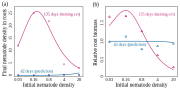
\includegraphics[width=\linewidth]{fig2.pdf} 
  \caption[Fit of the model to experimental data over one cropping
    season.]{Fit of the model to experimental data over one cropping
    season \citep{Ehwaeti1998}.  \textbf{(a)} Final density of
    nematodes in the roots and \textbf{(b)} relative biomass after 42
    (in blue) and 135 days (in magenta), as
    functions of the initial density of nematodes in the soil (log
    scale). Model outputs are shown as solid curves, circles and
    triangles represent experimental measurements.}
\label{fig2} 
\end{figure}

Parameters characterising virulent nematodes, \textit{i.e.}\ the fitness costs,  were selected from data on the \textit{Mi-1} resistant tomato  \citet{Castagnone-Sereno2007}. All parameters are summarised in \autoref{table1}.

\begin{table}[p]
  \small
  \caption{Model variables and parameters.}
  \label{table1}
  \begin{tabular}{@{}l@{ }l@{ }l@{ }l@{ }l@{ }l@{}}
    \hline
    Symbol & Description                      & Value(s) & & Unit &Ref.\\
    \hline
    $H^X$  & Density of healthy plant root    &          & & UR   & \\
    $P$    & Density of free living nematodes &          & & UN   & \\
    $E$    & Density of latently infected feeding sites& & & UR   &  \\
    $I$    & Density of infectious feeding sites &       & & UR   &  \\
    \hline
    $H_0$  & Initial root density & 6 &$(4.2,7.8)$ & UR & [1] \\
    $P_0$   & Initial nematode density in the soil & $0.8$ &$(0.03,20)$ & UN & [2] \\
    $p_v$ & Initial proportion of virulent nematodes & $10^{-3}$ &$(7\,10^{-4},1.3\,10^{-3})$ & -- & [3] \\
    $\beta$ & Infection rate & $1.11\,10^{-4}$ &$(7.78\,10^{-5},1.44\,10^{-4})$ & UR$^{-1}$ day$^{-1}$  & [*] \\
    $w_{\beta}$ & Fitness cost on infectiveness & $0.09$ &$(0.06, 0.12)$ & -- & [4] \\
    $\lambda$ & Transition rate from $E$ to $I$ & $0.06$ &$(0.042,0.078)$ & day$^{-1}$ & [4,5] \\
    $r$ & Nematode reproduction rate & $17$ &$(11.9, 22.1)$ & UN UR$^{-1}$ day$^{-1}$ & [4] \\
    $w_{r}$ & Fitness cost on reproduction & $0.31$ &$(0.22, 0.40)$ & -- & [4] \\
    $\delta$ & Fraction of  virulent offspring & $10^{-6}$ &$(7\, 10^{-7},1.3\,10^{-6})$ & -- & [3] \\
    $\alpha$ & Nematode mortality rate in roots & $0.125$ &$(0.0875, 0.1625)$ & day$^{-1}$  & [4,5] \\		
    $\eta$ & Nematode mortality rate in the soil & $0.04$ &$(0.028, 0.052)$ & day$^{-1}$ & [6] \\
    $\varphi$ & Between-season survival probability & $0.4$ &$(0.28, 0.52)$ & -- & [7] \\
    $\epsilon_y^X$ & Nematode infection success & \multicolumn{2}{@{ }l}{
                                                    \begin{tabular}[t]{@{}l@{}}
                                                      0 if $X=R$ and $y=a$\\[-6pt]
                                                      1 otherwise
                                                    \end{tabular}
    } & UR UN$^{-1}$  & \\		
    $\mu\,x$ & Plant root growth rate & $0.42$ &$(0.294, 0.546)$ &UR day$^{-1}$ & [1*]  \\
    $k$ & Nematode impact on root growth & $10.33$ &$(7.23,13.43)$ & -- & [*] \\ 
    $\tau$ &  Duration of a cropping season & $135$ & & days & [8] \\
    \hline
  \end{tabular}
  \par\medskip\footnotesize
  All parameters, except  $\epsilon_y^X$ and $\tau$, were varied for the sensitivity and robustness analyses: default value and $\pm 30\%$ variations  (indicated in brackets) were tested; larger variations were tested for $P_0$, in line with \citet{Ehwaeti1998}. \\
  \textbf{Units:} UR: number of feeding sites per gram of soil; UN: number of nematodes per gram of soil.  \\
  \textbf{Sources}: [1] \citet{Leskovar1990}; [2] \citet{Ehwaeti1998};
  [3] \citet{Ploeg1999}; [4] \citet{Castagnone-Sereno2007}; [5]
  \citet{Ekanayake1986}; [6] \citet{Tsai2008}; [7] Castagnone-Sereno, C.,
  unpublished data; [8] Djian-Caporalino, C., unpublished data; [8]
  Djian-Caporalino, C., unpublished data; [*] Estimated.
\end{table}

\subsection{Performance of resistance deployment strategies}
\label{sec:hrd}
We considered several resistance deployment strategies: the two
``pure'' resistant-only and susceptible-only strategies, consisting in
planting one crop type all the time; periodic rotation strategies,
alternating resistant and susceptible plants according to a repeated
pattern; and unconstrained strategies, \textit{i.e.}\ arbitrary
sequences of susceptible and resistant plants.

The performance of {each} strategy was quantified
with the ``healthy root density'' ($\overline{HRD}$), a proxy of
crop yield defined as the mean of the integral of healthy plant root
densities over the $n$ cropping seasons: 
\begin{equation}
  \overline{HRD}=\frac{1}{n} \sum_{i=1}^{n} \int_{i^{\text{th}}\text{ season}} H^{X}(t) dt
  \label{hrp}
\end{equation}
This quantity is similar to the healthy leaf area duration ($HAD$),
the integral of healthy green canopy area during a growing season,
used by many authors for airborne pathogens \citep{Waggoner1987,Gooding2000,vandenBosch2003,LoIacono2012,Elderfield2018,Papaix2018}.

The durability of resistance was then defined as the number of
consecutive seasons the resistant crop can be planted without losing
more than $1\%$ of crop yield ($\overline{HRD}$), compared to the
first year the resistance is used.  This definition is close to the
``usefulness time'' used in \citet{vandenBosch2008}, \textit{i.e.}\
the number of seasons until the yield drops under a preset
threshold. Such a metric helps assess the severity of the resistance
breaking problem at hand.

\subsection{Acceptable, efficient, and optimal strategies}

In order to quantify the benefit of each resistance deployment
strategy (or lack thereof), we computed its relative gain. It is
defined as the gain in healthy root density ($\overline{HRD}$) that
the strategy provides over the resistant-only strategy, normalised by
the gain that the resistant-only strategy provides over the
susceptible-only strategy.  This is illustrated in \autoref{fig3}.
For a given number of cropping seasons, \textit{i.e.}\ a given time
horizon, a positive relative gain indicates that the strategy
outperforms the resistant-only strategy, whereas a negative value
indicates that the resistant-only strategy is better. By definition,
the relative gain of the resistant-only strategy is equal to zero.
This metric is useful to determine whether, and how much, rotation
strategies are an improved way to deploy plant resistance. Moreover,
it allows comparisons across parameter values and epidemic situations
(see also \citet{Fabre2015}).

Based on this metric, we identified three types of strategies
(\autoref{fig3}). The optimal strategy is defined as the strategy that
maximizes the crop yield proxy $\overline{HRD}$~\eqref{hrp} and thus
the relative gain. Efficient strategies are defined as all strategies
that provide a relative gain at least $50\%$ as high as the optimal
strategy.  Last, acceptable strategies are all strategies with a
positive relative gain, \textit{i.e.}\ strategies that outperform
(even modestly) the resistant-only strategy.In what follows, the main
topic of interest will be to improve the efficacy of resistant-plant
based nematode control strategies. Therefore, we will essentially
concentrate on efficient and optimal deployment strategies.

In order to identify optimal periodic strategies, we computed all
periodic rotation strategies, beginning with resistant crops and
alternating $m$ and $p$ seasons of resistant and susceptible plants,
respectively. We denoted by $mR+pS$ these periodic strategies. As an
example, \autoref{fig3}a displays the healthy root density
($\overline{HRD}$) of all periodic rotation strategies over a
15-season time horizon. The optimal periodic strategy is $1R+5S$,
which corresponds to 1 season of resistant plants followed by 5
seasons of susceptible plants, and so on. A graphical representation
in \autoref{fig3}b--d displays the nematode and plant root dynamics
over time. We also identified unconstrained optimal strategies by
using a genetic algorithm implemented through the \textsc{genalg} R
package
(\href{https://CRAN.R-project.org/package=genalg}{https://CRAN.R-project.org/package=genalg}).
A chromosome in the genetic algorithm represented a full sequence of
susceptible ($S$, coded as 0) or resistant ($R$, coded as 1) plants
over the time horizon considered.  The population of chromosomes
(population size: 200) was initiated with random chromosomes. At each
generation, the best $20\%$ of chromosomes (according to our yield
proxy) were retained to form the next generation, with mutation
occurring at rate 0.01 (default parameter values of the package). The
algorithm was run for 50 generations, for each time
horizon. Convergence generally occurred in no more than 10
generations. The best chromosomes in the final generation were used to
determine the set of optimal unconstrained strategies.  We determined
optimal strategies for time horizons between 1 and 30 cropping
seasons. We also reported the corresponding ratios of resistant
plants, \textit{i.e.}\ the number of seasons with resistant plants
divided by the total number of seasons.

\begin{figure}[ht]
  \centering
   \includegraphics[width=\linewidth]{fig3.pdf} 
  \caption[Performance    of all periodic rotation strategies over a 15-season time horizon.]
  {\textbf{(a)} Performance ($\overline{HRD}$, colour scale)
    of all periodic rotation strategies, according to their number of
    seasons of resistant (in columns) and susceptible (in rows)
    plants, over a 15-season time horizon; performance of the
    susceptible-only, resistant-only and optimal strategies are
    indicated on the color scale.  The relative gain is defined as the
    gain in performance obtained by shifting from the resistant-only
    to another strategy, relative to the gain in performance obtained
    by shifting from the susceptible-only to the resistant-only
    strategy. The optimal periodic rotation strategy $1R+5S$ is
    identified by a black dot. Dotted$-$ and plain$-$line framed
    strategies represent acceptable periodic rotation strategies
    (relative gain $>0$) and efficient periodic rotation strategies
    (relative gain $>50\%$ of the optimal relative
    gain). \textbf{(b--d)} Graphical representation of two strategies:
    the resistant-only strategy (in blue) and the $1R+5S$
    periodic strategy (in gold), which is optimal over a
    15-season time horizon; shaded areas correspond to the inbetween
    seasons. Default parameter values were used (\autoref{table1}).  }
  \label{fig3}
\end{figure}

\subsection{Parameter exploration and epidemic scenarios}

To asses the impact of parameter values, we performed a global
sensitivity analysis \citep{Saltelli2008} on the healthy root density
$\overline{HRD}$~\eqref{hrp}, the yield proxy which quantifies the
performance of the resistance deployment strategies. We used the
multi-seasonal model~\eqref{sys1} and simulated the optimal periodic
rotation strategy over a 15-season time horizon. We varied all
parameter values by $\pm 30\%$ (default values given in
\autoref{table1}), except for the initial nematode density in the soil
$P_0$, for which larger variations were tested, in line with
\citet{Ehwaeti1998}. More details are available in Supporting
Information Methods~S3. The most influential parameters were found to
be the nematode reproduction rate $r$, the infection rate $\beta$, the
nematode mortality rate in the soil $\eta$ and the nematode mortality
rate in the root $\alpha$, four epidemiological parameters which
explained more than $80\%$ of the total $\overline{HRD}$ variability
(supporting information Fig.~S3). By varying these parameters around
their default value, we defined four epidemic scenarios, corresponding
to different levels of epidemic severity, from Low to Extreme
(\autoref{table2}).

\begin{table}[ht]
  \centering
  \caption{Definition of the four epidemic scenarios based on the four most influential  parameters: nematode reproduction rate ($r$), infection rate ($\beta$), nematode mortality in the soil ($\eta$) and in the roots ($\alpha$).}
  \label{table2}
  \begin{tabular}{lccccc}
    \hline
    Scenario & $\beta$ & $r$     & $\alpha$ & $\eta$  \\
    \hline
    Low      & $-30\%$ & $-30\%$ & $+30\%$  & $+30\%$ \\
    Medium   & --      & --      & --       &  --     \\
    High     & $+30\%$ & $+30\%$ & --       &  --     \\
    Extreme  & $+30\%$ & $+30\%$ & $-30\%$  & $-30\%$ \\
    \hline
  \end{tabular}
  \par\medskip\footnotesize
  Default parameter values (--) or default values $\pm 30\%$ were used (all values in \autoref{table1}).
\end{table}

Furthermore, we analysed with particular attention the influence of the genetic
parameters (fitness costs $w_{\beta},\,w_{r}$ and proportion of
virulent offspring $\delta$), possibly in combination with the
 epidemic scenarios, on the nature and  relative gain
of optimal rotation strategies. Specifically, we sought to determine
when optimal rotation strategies could outperform the usual
resistant-only strategy and to what extent crop yield could be
increased by using such rotation strategies.

\subsection{Robustness to parameter uncertainty}

Finally, we evaluated the robustness of our results to determine to
what extent optimal periodic strategies would remain effective if
biological parameters were not known with perfect precision. For the
medium, high and extreme epidemic scenarios defined in
\autoref{table2}, the optimal periodic strategy was computed over a
15-season time horizon and its performance was tested against
$\pm 10\%$, $20\%$ and $30\%$ variations of all parameters except the
initial nematode density in the soil $P_0$, for which larger
variations were tested (\autoref{table1}). In contrast with the
analysis focusing on the impact of the genetic parameters, the
periodic strategy was not computed afresh when the parameters
varied. For each epidemic scenario, we explored the parameter space
using a fractional factorial design containing 2187 parameter
combinations. The design was obtained using the \textsc{planor} R
package
(\href{https://CRAN.R-project.org/package=planor}{https://CRAN.R-project.org/package=planor}).


% ****************   SECTION RESULTS  ***************%

\section{Results}
\label{sec:Res} 

\subsection{Optimal and efficient deployment strategies} \label{sec:optimal_eff}

The performances (crop yield proxy $\overline{HRD}$) of
pure, optimal and efficient deployment strategies are shown
in \autoref{fig4}a, for different time horizons and the default
parameters. As expected, the resistant-only, efficient and
optimal strategies outperformed the susceptible-only strategy, since
the deployment of resistance prevents infection by avirulent
nematodes. However, for these strategies, {the crop yield proxy}
decreased with the time horizon. This is also expected, as the
deployment of resistance also causes virulent nematodes to appear and
take over the nematode population.

\begin{figure}[htp]
  \centering
  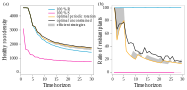
\includegraphics[width=\linewidth]{fig4.pdf} 
  \caption[(a) Performance and
    (b) ratio of resistant plants as functions of the time
    horizon, for different deployment strategie]{\textbf{(a)} Healthy root density ($\overline{HRD}$) and
    \textbf{(b)} ratio of resistant plants as functions of the time
    horizon, for different deployment strategies: susceptible-only
    (magenta), resistant-only (blue), efficient periodic rotations (grey
    area), optimal periodic rotation (gold) and optimal
    unconstrained (black). Different unconstrained optimal strategies
    (yielding the same $\overline{HRD}$) were identified, so the ratio
    of resistant plants is represented in panel (b) by its average
    value (the ratio range is represented in Supporting Information Fig.~S2). Default parameter values were used (\autoref{table1}).}
\label{fig4} 
\end{figure}

For up to five years of cultivation, the resistant-only strategy
performed as well as any optimal deployment strategy, but over longer
time horizons, it could be significantly outperformed. For instance,
over 15 cropping seasons, the {healthy root density} was around
$2044$~UR.day for optimal strategies, while it had dropped to
$1822$~UR.day for a pure resistant-only strategy (\autoref{fig4}a). By
definition, efficient periodic rotations performed better than the
resistant-only strategy and were worse than but close to the optimal
periodic rotation.  Interestingly, for all time horizons considered
(up to 30 years), the optimal periodic and the unconstrained
strategies had almost identical performances. This indicates that
periodic rotations are almost optimal in this system.

The deployment of a pure resistant-only strategy is thus reasonable
for at most five years in this cropping system. Beyond that, the
optimal strategy generally was to alternate one season of resistant
plants with a few seasons of susceptible plants, as shown for instance
in \autoref{fig3} for a 15-season time horizon. This optimal strategy
ensures that virulent nematodes remain sufficiently rare in the soil,
{sustaining} the efficiency of resistant plants, which severely reduce
the avirulent nematode population. Other periodic rotations
outperformed the resistant-only strategy. Yet, while there was
generally one single optimal periodic rotation strategy for a given
time horizon and parameter set, there were only a few acceptable and
even less efficient rotation strategies (\textit{e.g.}~10 acceptable
and 5 efficient strategies out of 105 periodic rotation strategies;
\autoref{fig3}a).


For a given time horizon, the average ratio of resistant plants
{characterizing} the unconstrained optimal strategy {was generally
  higher} than for the optimal periodic rotation strategy; for
acceptable and efficient periodic rotations, the ratio also tended to
be slightly higher than for the optimal periodic rotation
(\autoref{fig4}b).  For instance, over a 15-season time horizon, the
genetic algorithm identified 11 equivalent solutions and the ratio of
resistant plants deployed was on average $30\%$. For the optimal
periodic strategy, it was only $20\%$ and for acceptable and efficient
periodic rotation strategies, it ranged between $20\%$ and
$27\%$. Unconstrained optimal strategies identified by the genetic
algorithm were actually fairly similar to optimal periodic rotations
in terms of structure, except that more resistant plants were used in
the final seasons, explaining the higher ratio of resistant plants in
unconstrained strategies.

\subsection{Influence of fitness costs}

We computed the optimal periodic rotation strategies as functions of
the two fitness costs on infectiveness ($w_{\beta}$) and reproduction
($w_{r}$), to explore their effects on the two metrics defined above:
the relative gain brought about by optimal periodic rotations and the
resistance durability. Results are displayed in \autoref{fig5}a.

\begin{figure}[ht]
  \centering
   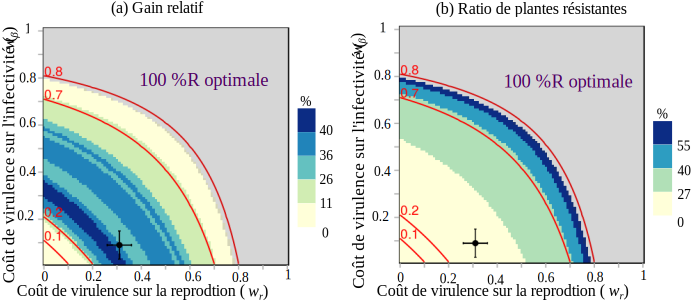
\includegraphics[width=\linewidth]{fig5.pdf} 
  \caption[(a) Relative gain and (b) ratio of
    resistant plants as functions of the two fitness costs, for
    optimal periodic strategies computed over a 15-season time
    horizon.]{\textbf{(a)} Relative gain and \textbf{(b)} ratio of
    resistant plants as functions of the two fitness costs, for
    optimal periodic strategies computed over a 15-season time
    horizon. The grey area corresponds to fitness costs for which the
    resistance was fully durable over the 15-season time horizon.
    Level curves in red represent different values of the effective
    fitness cost $w^*$ defined in \eqref{eff_w}. The black
    dot and the error bars indicate the default fitness costs and
    their standard deviations \citep{Castagnone-Sereno2007}.}
  \label{fig5}
\end{figure}

The area where resistance was durable for (at least) the entire
15-season time horizon is found in the upper right part of the figure.
This area corresponds to R-genes associated with very strong
fitness costs of one or the other kind ($w_{\beta}\geqslant 0.8$ or
$w_{r}\geqslant 0.8$). This means that rotation was unnecessary in such
conditions, at least for the time horizon considered. For lower
fitness costs, resistance was not durable and thus the use of optimal
periodic rotation strategies produced a better crop yield than the
resistant-only strategy (positive relative gain).

The relative gain was fairly high, except in two cases. On the one
hand, when resistance breaking entailed low fitness costs
($w_{\beta}$ or $w_{r}\leqslant 0.12$), the relative gain was almost
zero. This is not surprising since for such low fitness costs,
virulent nematodes cannot be prevented from overturning the nematode
population, even with rotation strategies, as they develop quite well
on both resistant and susceptible plants. Cropping resistant plants is
then useless and does not provide any increase in yield.  On the other
hand, R-genes associated with high fitness costs
($w_{\beta}$ or $w_{r}\geqslant 0.7$) provided a relative gain of less
than $10\%$. For such fitness costs, resistance durability was in fact
quite high (12 to 14 seasons). Therefore, the resistant-only strategy was quite efficient and
the additional yield provided by periodic rotations is minimal.

Significant relative gains are thus observed for R-genes inducing
medium fitness costs in virulent nematodes. Relative gains can in this
case reach values up to $50\%$. Interestingly, in the literature the
  fitness cost on reproduction $w_{r}$ is estimated between $0.26$ and
  $0.36$ and the fitness cost on infectiveness $w_{\beta}$ between $0.03$
  and $0.15$, for the susceptible Saint Pierre tomato cultivar \citep{Castagnone-Sereno2007}. For
such realistic fitness cost values, the expected relative gain that
could be realised by switching from a resistant-only strategy to an
optimal periodic rotation would be between $26\%$ and
  $43\%$  with a relative
gain equal to $28\%$  for the default values parameter values.

The ratio of resistant plants deployed in the optimal periodic
rotation strategies in order to achieve such relative gain values were
remarkably low, lying between $13\%$ and $27\%$
(\autoref{fig5}b). For the default parameter values, the
ratio of resistant plants was $20\%$. The ratio of
resistant plants used in the optimal rotation strategies increased
with the values of the fitness costs.

Interestingly, \autoref{fig5} shows that the fitness cost
distribution between infectiveness and reproduction is important for
crop yield. Indeed, even though the two fitness costs had perfectly
symmetrical effects, the level curves of both the relative gain and
the ratio of resistant plants were markedly concave. Therefore, a
balanced distribution of fitness costs (\textit{e.g.}\
$w_{\beta}=w_{r}=0.4$) could lead to a situation where resistance was
not durable, while an uneven distribution (\textit{e.g.}\ $w_{r}=0.8$,
$w_{\beta}=0$) could lead to a durable situation. The two fitness
costs thus did not act in an additive manner and interacted
negatively.  The derivation of the multiseason basic reproduction
number $R_{0}$ of virulent nematodes revealed that it depended only on
the product $(1-w_{\beta})(1-w_{r})$ (Supporting Information Methods~S1).  We hence defined an ``effective'' fitness cost as:
\begin{equation}
  w^{*}=1-(1-w_{\beta})(1-w_{r})=w_{\beta}+w_{r}-w_{\beta}w_{r},
  \label{eff_w}
\end{equation}
whose level curves perfectly reflected the level curves of the
relative gain and ratio of resistant plants
(\autoref{fig5}). The performance of resistance-based
strategies therefore appeared to be entirely determined by this
quantity.

In the following, we thus present results in terms of this effective
fitness cost $w^{*}$.

\subsection{Interplay between epidemic scenarios and  genetic parameters}

We studied the influence of the genetic parameters in interaction with
the epidemic scenarios on the relative gain and
durability. \autoref{fig6} shows the relative gain obtained for a
15-season time horizon as a function of the effective fitness cost
($w^*$), for different values of the fraction of virulent offspring
($\delta$) and the four epidemic scenarios. Parameter ranges ensuring resistance durability
over the 15-season time horizon were identified (grey areas).
$\delta$ had no effect on durability according to our
definition. Indeed, when only resistant plants were deployed,
avirulent nematodes could not reproduce. The resistance was durable as
the effective fitness cost $w^*$ {overshot} a given threshold, which
strongly increased with the severity of the epidemic scenario.  For
instance, for {low epidemic severity}, R-genes
associated with effective fitness costs between $0.30$ and $1$ were
durable (\autoref{fig6}a), while in the Extreme scenario, they
were durable only for fitness costs larger than $0.95$
(\autoref{fig6}d).

\begin{figure}[htp]
  \centering
   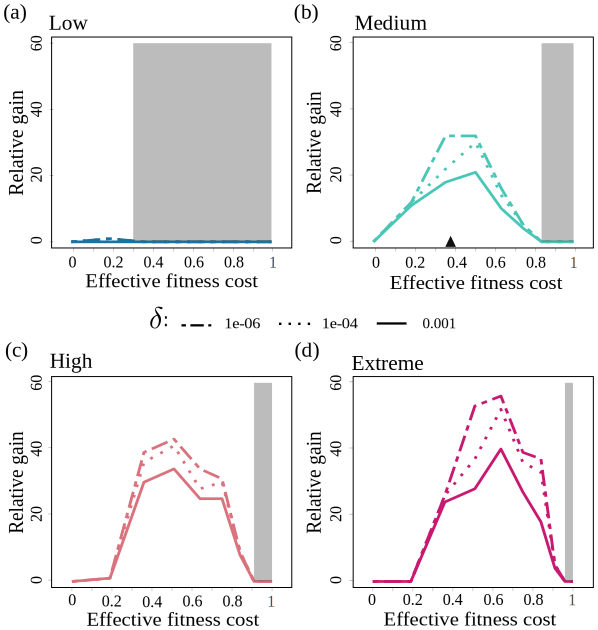
\includegraphics[width=.9\linewidth]{fig6.pdf} 
  \caption[Graphical representation of the relative gain for a
    15-season time horizon as function of epidemic scenarios]{Graphical representation of the relative gain for a
    15-season time horizon for the four epidemic scenarios
    (a-d) defined in \autoref{table2}, as a function of the effective
    fitness cost ($w^*$) and the fraction of virulent offspring
    ($\delta$). The default effective fitness cost $w^*=0.37$ is
    represented by the black triangle 
    \citep{Castagnone-Sereno2007}. Grey areas represent the values of
    $w^*$ for which the resistance was durable over the 15-season time
    horizon.}
  \label{fig6}
\end{figure}

The relative gain varied significantly according to the genetic
parameters and epidemic scenarios, except for the 
{Low epidemic scenario} where it remained close to zero
(\autoref{fig6}a). In this case, nematode infestation remained
very low so that the resistant-only strategy actually provided very
good control. The relative gain increased with {epidemic severity}
and decreased with the fraction of virulent offspring $\delta$. The
best gains were found for R-genes associated with medium to high
effective fitness costs (between $0.4$ to $0.65$). For example, an
extreme {severity} combined with a low fraction of
virulent offspring $\delta=10^{-6}$ and a fitness cost $w^*=0.65$
yielded a relative gain of up to $58\%$
(\autoref{fig6}d). Hence, {epidemic severity} tended to
increase the advantages of cultivar rotations over the resistant-only
strategy.

\subsection{Robustness of deployment strategies}

Finally, we evaluated the robustness of the optimal periodic rotation
strategies by testing their efficacy against variations in parameter
values.  \autoref{fig7} represents the relative gain when deploying
the optimal periodic strategy, computed over a 15-season time horizon
and for the default parameters corresponding to the three epidemic
scenarios, in the face of increasing levels of parameter variations.
Such variations can effectively render the computed rotation
strategies sub-optimal.

\begin{figure}[htp]
  \centering
   \includegraphics[width=.9\linewidth]{fig7.pdf} 
  \caption[Robustness of the relative gain to variations in model
    parameters]{Robustness of the relative gain to variations in model
    parameters, for three epidemic scenario (Medium, High, Extreme)
    and three levels of parameter variations ($\pm 10\%$, $20\%$,
    $30\%$, and variations in the initial nematode density as reported
    in \autoref{table1}). For each scenario, the optimal periodic
    strategy, computed for a 15-season time horizon and default
    parameters values (Tables~\ref{table1}--\ref{table2}) was
    applied. The relative gain of this strategy was computed for all
    parameter combinations within each level of parameter
    variations. In each case, the relative gains obtained for the
    default parameter values (black diamond) and for the different
    parameter combinations (2187 coloured dots) were plotted. Violin
    plots were drawn to help quantification, with horizontal bars
    indicating the median (thick line), first and third quartiles
    (thin lines). The percentages provided on the bottom line
    correspond to the fraction of parameter combinations which yield
    non positive relative gains, \textit{i.e.}\ for which the optimal
    strategy would not be acceptable (\autoref{fig3}).}
  \label{fig7} 
\end{figure}

In a large majority of cases, the relative gain remained positive,
although it declined, as expected, with the level of parameter
variations.  In the Medium epidemic scenario, most parameter
combinations decreased the relative gain below the $28\%$ gain
predicted for default parameter values (black diamond in
\autoref{fig7}). The median relative gain was between $8$ and $20\%$,
depending on the level of parameter variations. Note however
that some parameter combinations actually resulted in
higher-than-expected relative gains.  The situation was even more
favourable in the High and Extreme epidemic scenarios, for which the
decline in relative gain was less pronounced. In addition, a
significant fraction of parameter combinations caused an increase in
the relative performance of the optimal rotation strategy
(\autoref{fig7}).

Parameter combinations causing the rotation strategy to become
non-acceptable, \text{i.e.} for which the strategy failed to provide a
positive relative gain, were rare overall, especially for the most
severe epidemic scenarios. At most, these combinations represented
$18\%$ of all combinations (for $\pm 30\%$ variations in the Medium
epidemic scenario). The optimal strategy $1R+5S$, even in the face of
important parameter uncertainty, thus retained higher performance than
the resistant-only strategy in more than $82\%$ of the cases
tested. In that sense, the relative performance of the optimal
periodic strategy was globally very robust to parameter changes.


 

% *****************   SECTION DISCUSSION  ***************%

\section{Discussion}

\subsection{Crop rotation is an efficient strategy} \label{discussion:part1}

The present study was based on a new model of plant–nematode
interactions parameterized from the literature and fitted to
experimental data, so as to be representative of the tomato/root-knot
nematode system. As a key result, we found that alternating
susceptible and resistant plant cultivars in time can help limit the
proportion of virulent individuals in nematode populations and thereby
reduce crop loss substantially. According to our
simulations, relative gains as high as $40\%$ can be achieved,
compared to the baseline strategy of deploying only resistant plants,
over time horizons of 15 years or more.

The relative gain achievable with optimal crop rotations was found to
be greatest for high or extreme epidemic scenarios, \textit{i.e.}\  for
high {epidemic severities}. The latter result echoes previous findings
on the influence of epidemic intensity on resistance durability in the
context of spatial mixtures \citep{vandenBosch2003,Fabre2012}.  The
gain also increased, to a smaller extent, if the fraction of virulent
offspring in avirulent egg-clutches is smaller, and if the culture is
sustained over longer temporal horizons. Remarkably, the relative gain
obtained from virulence costs similar to those estimated for the
\textit{Mi-1} resistant gene is close to the maximum achievable gain
value (\autoref{fig5}a), suggesting that crop rotation is a
particularly promising strategy when deploying \textit{Mi-1}
cultivars.

We also found that periodic crop rotation strategies are almost as
effective as free (unconstrained) alternation strategies. This result
has considerable importance, since periodic rotation patterns are
in real-world applications much easier for crop growers to implement
than complicated unconstrained sequences. 

Few recent theoretical studies have considered the deployment of
different cultivars over time. One is
\citet{Rimbaud2018}, that compared four resistance deployment
strategies of major resistance genes: mosaics, mixtures, rotations and
pyramiding, to manage cereal rust fungi in agricultural landscapes
durably. They found cultivar rotation to be the most efficient in the
long-term, once every R-genes had been overcome. In a study of plant
virus epidemic control by mixing resistant and susceptible cultivars
in space and time, \citet{Fabre2015} identified that in more than
$20\%$ of the scenarios considered, optimal strategies involved
cultivar rotation at the landscape scale. Studies are even scarcer
regarding {root-knot nematodes}, for which the literature on cultivar rotation is
essentially experimental. For these low-dispersing soil-borne pests,
data support our modelling predictions in suggesting that rotations
are an effective way to reduce yield losses and to delay outbreaks
\citep{Tzortzakakis2000,Miller2006,McSorley2011}.  For instance,
\citet{Djian-Caporalino2014} experimentally compared the performance
of several strategies to control {root-knot nematodes} in vegetable cropping systems,
including rotations of two major R-genes in pepper cultivars, over
three years. They reported that cultivar rotation can improve
epidemic control and resistance durability. Another study by
\citet{Talavera2009} on {root-knot nematode} management compared the effects of four
crop rotations between resistant and susceptible tomato plants in a
three-year field experiment. Regarding crop yield and durability, this
study showed that the best strategy consisted in growing two resistant
cultivars, followed by one susceptible cultivar. This is strikingly
consistent with our modelling predictions, since we found that the
yield-maximising strategy, over a three-season temporal horizon, is
$2R + 1S$ (\autoref{fig4}b). Our modelling results further indicate
that the performance of crop rotations for {root-knot nematode} control would be even
more pronounced over longer time horizons.

\subsection{Crop rotation (usually) requires low ratios of resistant plants}  \label{sec:discussion-lowratio}

Interestingly, the optimal rotation strategies identified in this study
were characterised by relatively low ratios of resistant plants, as
soon as the temporal horizon exceeded seven cropping seasons (\autoref{fig5}b).
Since avirulent nematodes thrive on susceptible plants, low ratios
of resistant plants are expected to increase crop loss, especially
in the short-term. However, in the longer term, low ratios limit selection
for virulent variants, thus prolongating the efficacy of resistant
plants when those are deployed. For {root-knot nematodes}, it appears that the relatively
fast within-season epidemiological dynamics sets the optimal balance
between the two effects at a low ratio of resistant plants. Our results
are consistent with \citet{vandenBosch2003}, who showed that, in
many instances, low ratios allowed to make the most of resistance,
by reducing the selection pressure for virulent pathogens and promoting
resistance durability.

Interestingly, studies of spatial deployment strategies tend to report
higher optimal ratios of resistant plants. \citet{Fabre2012}, working
on plant resistance to viruses, demonstrated that optimal ratios were
frequently over $50\%$. For instance, for low fitness costs, the
ratio ranged between $50$ and $70\%$, depending on the epidemic
profile. Regarding phytopathogenic fungi, \citet{Papaix2014} also
found that high ratios combined with low levels of variety aggregation
provided optimal control of the fungi in agricultural landscapes.
Therefore, the selection pressure in favour of virulent variants seems
to be lower when mixing resistant and susceptible cultivars in space
compared to alternating them over time.

It should be remarked that low ratios of resistant plants are in total
contrast with the currently dominant agricultural practices, based on
the regular cropping of tomato cultivars bearing the same
\textit{Mi-1} resistance gene. Indeed, growing resistant tomatoes is
the best strategy over a single cropping season. However, be it in the
field or in experimental studies, such resistant-only strategies often
fail, and virulent {root-knot nematodes} overcoming resistance have
been observed in most tomato growing areas worldwide \citep{Seid2015}.
More specifically, experimental findings have shown that three
consecutive cropping seasons of the \textit{Mi-1} gene in tomatoes
were enough for {nematodes} to overcome the resistance
\citep{Eddaoudi1997,Verdejo-Lucas2009}.  These findings are consistent
with our results when fitness costs are not too severe, close to
available experimental estimates \citep{Castagnone-Sereno2007,
  Djian-Caporalino2011}.  The intense deployment of resistant
cultivars is thus bound to cause boom and bust cycles in this system
\citep{Brown2011}. During the boom, crop yield increases rapidly
thanks to the use of new resistant cultivar by growers and
farmers. Nevertheless, it is followed by a bust, characterised by the
rapid breakdown of the resistance by virulent variants and a drop in
crop yield. The switch to a new cultivar, carrying a fresh resistance
gene, then triggers a new cycle. To break this cycle and preserve the
efficiency of resistance genes, which are scarce and valuable
resources, cultivar rotations such as the ones proposed in this study
are a feasible and sustainable alternative. However, convincing
growers to switch from a short-term to a long-term perspective may be
an issue. It would require close interactions between scientists and
growers to co-design acceptable resistance deployment strategies.

\subsection{What makes a good resistance gene?}

We investigated the effects of varying three mechanistic parameters
characterizing how a resistance gene behaves with respect to
resistance breaking by {nematodes}: the fitness cost it imposes on the
infectivity of virulent nematodes ($w_{\beta}$), the fitness cost it
imposes on their reproduction ($w_{r}$), and the frequency of
virulence appearance in avirulent clutches ($\delta$). Obviously, one
would seek R-genes that, when overcome, would generate high values of
the first two parameters, and low values of the third, even
  though it may not necessarily be easy to evaluate.

Our results showed that the two fitness costs had interchangeable
effects in shaping the population dynamics of virulent
variants. However, the two costs interacted negatively, as the benefit
of increasing one fitness cost was reduced when the other fitness cost
is already high (\autoref{fig5}a). This original result
implies that, when evaluating the potential of resistance
genes to improve durability, breeders should seek and introgress
R-genes with maximal fitness cost on either one or the two components
of the nematode life-cycle (reproduction or infectivity), rather than
a balanced distribution of the two types of costs. To help address the
existence of two different types of fitness costs, a specificity of
our model, we derived a simple formula to synthesize the two fitness
costs into one effective fitness cost, according to which different
resistance genes can be ranked in terms of their
durability. Comparatively, the rate of production of virulent
nematodes $\delta$ had virtually no impact on the durability of
resistance genes.

Rotation strategies provided the largest relative
benefits over the resistant-only strategy for intermediate fitness
costs. Such measurements are not always easily accessible in the literature,
but this property seems to hold in a few other studies. For instance,
a reinvestigation of the simulation data on plant virus epidemics
obtained by \citet{Fabre2012} for high epidemic intensities showed
that the best relative gains were obtained for intermediate fitness
costs. Another study by \citet{Rousseau2019} showed that relative
additional gains, provided by combining quantitative and qualitative
resistances over qualitative resistances only, were most noticeable
for intermediate fitness costs. In both studies, the reasons for this
were similar to the present study: high fitness costs induced durable
resistance so that the yield could only be marginally increased, whereas
low costs induced poorly efficient resistance that did not benefit
from an optimal deployement. R-genes associated with intermediate
fitness costs are thus the ones that could benefit the most from improvements
in terms of deployment or cultivar genetic background.

\subsection{Optimal rotations in practice} \label{sec:discussion-OptRot-in-practice}
 
A major outcome of this work would be to recommend custom optimal
resistance deployment strategies to crop growers, depending on the
temporal horizon sought, but also on the epidemic context, the R-genes
to be deployed, and on the agricultural practices that determine model
parameter values. Indeed, even though optimal resistance deployment
has been proven to be efficient, quite few periodic rotation
strategies are actually ``acceptable'' and even less are ``efficient"
(\autoref{fig3}a). The pattern of the rotation, in particular the
ratio of resistant plants, is critical. In addition, soil infestation
and epidemiological or genetic parameters are particularly difficult
to estimate, and likely subject to considerable uncertainty. For
instance, \citet{Djian-Caporalino2011} found a large variability in
the fitness costs on reproduction. To address this issue, we simulated
the use of optimal periodic strategies, as computed for default
parameter values, and investigated how their performance responded to
parameter variations. We found that the relative gain was globally
robust to parameter changes. Thus, optimal periodic rotations can
outperform the resistant-only strategy in terms of crop yield even if
the relevant parameters are known imperfectly. Rotating susceptible
and resistant cultivars is not necessarily a good idea. However,
rotating wisely (optimally) can provide significant gains and is
robust to parameter uncertainties, which is a very desirable property
in practice.

There are still few studies that investigate the
robustness of resistance deployment strategies, or more generally
plant pathogen control methods. A similar analysis to parameter
misspecification was conducted by \citet{Hyatt-Twynam2017} to assess
the performance of optimal strategies to control the spread of citrus
canker in Florida, using one at a time epidemiological parameter
changes. In the context of fungicide resistance management,
\citet{Elderfield2018} found that mixtures always outperformed
alternations when parameters varied, but not the deployment
strategy. More such studies should arise to help bridge the gap
between theoretical resistance deployment strategies and their
implementation in the field.

Optimal strategies could feature high year-to-year variations in
yield, which may not be economically viable for farmers. Taking
advantage of the limited mobility of nematodes, this issue could be
adressed by implementing asynchronous crop rotation strategies in
different rows or plots, provided that contamination between those be
carefully avoided. The seasonal yield variations in each row would
average out, ensuring a more stable income for farmers while achieving
the performance of the optimal rotation strategy.

Although nematode resistance in general can be conferred by single
major genes or by combinations of genes or quantitative trait loci
(QTL), root-knot nematode resistance in solanaceous crops mainly
relies upon single major dominant genes
\citep{Barbary2015}. Currently, \textit{Mi-1} is the only resistance
gene used in tomato cultivars, which makes this study particularly
relevant for the tomato/root-knot nematode pathosystem. In pepper,
though, QTL have recently been identified \citep{Barbary2016} and
their efficiency was demonstrated in laboratory experiments
\citep{Barbary2014}. As such they could be a promising source of
resistance, alone or in combination with major R genes, which would
deserve further modelling investigations along the lines of the
present study. An ideal strategy would be to breed tomato varieties
with unbreakable resistance. In the absence of such a silver bullet, rotation of
varieties seems a viable alternative.

Provided sufficient parameter estimates are available, the model could
effortlessly be extended to simulate rotations of tomato with other
species (e.g.\ other Solanaceae or cucurbits), as is common in many
cropping systems. The present model could also readily be extended to
incorporate different R-genes and serve as a basis to evaluate more
complex resistance deployment strategies, involving rotations between
susceptible and several resistant cultivars or species, including
pyramided ones.


% ***************   ACKNOWLEDGEMENTS    ***************%

\section*{Acknowledgements}

This work was funded by INRAE and Région Sud PACA, France. It was certified by the Terralia-PASS competitiveness research cluster. The authors are grateful to the Inria Sophia Antipolis -- Méditerranée ``NEF'' computation cluster for providing resources and support.


\section*{Data availability statement}
The data that support the findings of this study are available from the corresponding author upon reasonable request.
 %sans .tex

	%%%%%%%%%%%%%%%%%%%%%%%%%%%%%%%%%%%%%%%%%%%%%%%%%%%%%%%%%%%%%%%%%%%%%%%%%%%%%%%%%%%%%%%%%%%%%
	%%									Chapitre 4						%
	%%%%%%%%%%%%%%%%%%%%%%%%%%%%%%%%%%%%%%%%%%%%%%%%%%%%%%%%%%%%%%%%%%%%%%%%%%%%%%%%%%%%%%%%%%%%%
	
	\selectlanguage{french} %ou english
	\renewcommand{\tablename}{Tableau}
	\renewcommand{\figurename}{Figure}
	
	{\chapter{Approches expérimentales de la dynamique des nématodes} \label{chapter4} 
		\label{chap:experimentation}}
	
		\minitoc
		\newpage
		
	
		
	%%%%%%%%%%%%%%%%%%%%%%%%%%%%%%%%%%%%%%%%%%%%%%%%%%%%%%%%%%%%%%%%%%%%%%%%%%%%%%%%%%%%%%%%%%%%%
	
	
\section[Dynamiques expérimentales d'infection de tomates sensibles par \textit{M.  incognita}]{Dynamiques expérimentales d'infection de tomates sensibles par \textit{Meloidogyne  incognita} dans les racines et le sol} \label{sec:experimentation}
	
	
	
\subsection{Introduction}
	
	La tomate (\textit{Solanum lycopersicum}) originaire d’Amérique du sud  est le deuxième légume le plus consommé au monde, juste après la pomme de terre.
Par exemple, il s’agit du premier légume consommé par les français en volume selon les données recensées par le Kantar Worldpanel entre 2012 et 2014.  Sa consommation moyenne annuelle  par ménage \footnote{qui représente 2,3 personnes selon Insee} était de 13,9 kg. La production mondiale de tomates a progressé régulièrement au cours du XXe siècle et s'est accrue considérablement durant les trois dernières décennies. En 2017, 182  millions de tonnes de tomates ont été produites dans plus de 170  pays  \citep{FAOstat2018}. 
	
	 Cependant, la tomate  est une espèce de plante  sensible aux attaques des nématodes
du  genre \textit{Meloidogyne} \citep{Divito1979, Seid2015}. Au niveau économique, les pertes annuelles mondiales seraient estimées à 4,3 milliards d’euros \citep{McCarter2009}. 
Plus particulièrement, les nématodes à galles de l'espèce \textit{ M. incognita }  (\textcolor{RoyalBlue}{Kofoid \& White, 1919})  peuvent causer jusqu’à 27 \% de pertes de rendements pour les cultures de tomate. La lutte la plus efficace est l'utilisation de cultivars de tomates résistantes portant un gène R (le gène \textit{Mi}). Durant ma  thèse, un des objectifs de notre travail a été de rechercher par
modélisation de la dynamique plante-nématodes les stratégies optimales de déploiement des
plantes résistantes, basées sur l'alternance dans le temps de plantes résistantes et de plantes sensibles. 
	
	Pour cela nous avons construit un modèle décrivant la dynamique saisonnière d'une
population de nématodes à galles à l'échelle d'une plante.  Les paramètres du modèle ont été obtenus à partir de données publiées (\autoref{table1} du \autoref{chapter_3}). %(\autoref{table1}).
Cependant, nous ne disposons pas de données pour 3 paramètres.
Nous avons obtenu leur valeur en procédant à l’ajustement de notre modèle aux données expérimentales, issues d’\citet{Ehwaeti1998}. Cette étude décrit l’infection de plantes de tomates sensibles \textit{cv. Moneymaker}   par des nématodes \textit{M. incognita}
	avirulents. Bien que l'ajustement de notre modèle était fidèle aux données de l'expérience, nous voulions acquérir des données supplémentaires pour tester  l'ajustement du modèle dans des conditions différentes.
	
	De même, les données sur la relation entre les densités initiales de \textit{M.
incognita} et les rendements de tomates  et /ou la densité finale de nématodes dans le sol étaient peu nombreuses \citep{Wesemael2011, Greco2010}. 
\citet{Vito1991} ont trouvé que la population finale de nématodes déclinait lorsque la densité initiale de nématodes dans le sol était plus grande.
Effectivement, quand l'infection est trop importante au commencement, la plante ne pousse presque pas, donc les nématodes ne peuvent pas se multiplier.
Les auteurs ont également montré que la densité de nématodes initiale affectait aussi négativement  le rendement des tomates ($e.g.$ taille de la tomate).
	
	Nous avons donc  conduit notre propre expérience pour produire des données pour  tester l'ajustement du modèle pour une situation épidémiologique différente.
L'objectif principal de cette section est de présenter l'expérience qui nous a permis de récolter des données expérimentales reflétant la dynamique de l'interaction entre une tomate sensible  et des nématodes avirulents.
	Plus précisément, nous avons analysé la densité finale ($P_f$)  de nématodes dans le sol et la biomasse relative ($i.e.$ la masse de racines fraîches infectées par   les nématodes divisée par la moyenne des masses de racines fraîches sans infestation) après 35 jours de culture, sur des plantes de tomates inoculées avec différentes densités initiales de \textit{M. incognita} ($P_i$).  Cette expérience est très similaire à celle de \citep{Ehwaeti1998}. 
	
\subsection{Matériel et Méthode} 
	
	
\subsubsection{Matériel végétal}
	
	Nous avons utilisé comme lignée de tomate le cultivar  sensible, Saint Pierre, d'intérêt agronomique et commercial très important.
C'est une tomate pratiquement ronde, rouge, de 100 à 140 grammes à chair ferme et très parfumée 
(\autoref{tomate}).

		\begin{figure}[H]
			\centering \includegraphics[width=0.6\linewidth]{saint_pierre.jpg}
			\caption{ Tomate de la variété Saint Pierre \protect\footnotemark.}
	        \label{tomate}
		\end{figure}
		\footnotetext{\href{https://www.jardiner-malin.fr/fiche/culture-tomate.html}{https://www.jardiner-malin.fr/ 
		fiche/culture-tomate.html}}
			  
La tomate appartenant à la famille des \textit{Solanaceae},
elle est apparentée à de nombreuses plantes  (poivron, pomme de terre, aubergine, tabac).
Ainsi dans une certaine mesure, les connaissances acquises grâce aux études menées sur la tomate peuvent être  appliquées à ces plantes.  Par ailleurs le cultivar Saint Pierre est utilisé en routine pour les élevages de nématodes à galles. La culture est donc maîtrisée et la durée du cycle de \textit{M. incognita} est connue pour cette plante.
Pour toutes ces raisons, la tomate est un excellent  modèle d'étude / matériel de recherche  pour la famille des \textit{Solanaceae}.
	
\subsubsection{Les nématodes}
	Les nématodes  utilisés dans cette étude proviennent d’une collection maintenue
	dans l'UMR ISA  (INRAE 1355 PACA, site de Sophia Antipolis; CNRS 7254; Université Côte d'Azur), dans le Sud-Est de la France. Cette
collection comprend environ 80 souches de \textit{Meloidogyne}, issues du monde entier,
représentatives des espèces les plus nuisibles. Une  souche
avirulente vis-à-vis du gène $Mi$-$1$ de la tomate a été utilisée dans cette étude. La souche \textit{M. incognita} Morelos  (espèce originaire du Mexique) a
été utilisée dans cette expérimentation  qui a pour but  de quantifier les dégâts que causent l'infestation de racines de tomates sensibles  par les nématodes.   
Pour les besoins de notre expérience nous avons au préalable produit une quantité abondante de nématodes \textit{M. incognita} (voir \Cref{secan1}). 
	
	
\subsubsection{Déroulement de l'expérience}
	Au début de l'expérience ($t=0$), nous avions à notre disposition $40$ plantes âgées de $42$ jours cultivées dans des  pots en plastique de dimension 9x9x9 cm  remplis d'un mélange de
sol stérilisé et sableux. La masse de sol dans chacun des $40$ pots   était de $470$ grammes.  
Ces plantes étaient maintenues dans une chambre climatique  en conditions contrôlées  à  
24$^{\circ}$ C, avec un éclairage artificiel ($16$ h de jour et 8 h de nuit) et une humidité relative de $60$ à $70$ \%.  L’arrosage était manuel. 
Les $32$ plus belles plantes ont été conservées pour l'essai.
Les densités de populations de nématodes initiales ($P_i$)  testées étaient de $0$; $0,6$; $8$ et
$16$  nématodes de stade J2 / g de sol (UN).   
Nous avons effectué huit réplicats par modalité d'inoculum et randomisé les positions des plantes sur le tablar.   En effet, bien que les plantes aient été placées en conditions contrôlées, des différences dans la taille des racines et des plants subsistent, pouvant entraîner des différences de mesures au sein de la même modalité d'inoculation, en interaction potentielle avec des effets de bordure, d'éclairage ou d'arrosage. En randomisant les plantes sur le tablar, ces effets étaient homogénéisés sur toutes les modalités. Les plantes  ont été récoltées  35 jours après inoculation afin d'évaluer l'effet des nématodes sur la croissance de la plante et de comparer nos données à celle de \citet{Ehwaeti1998}. Les plantes ont été repiquées dans des pots et des sols avec différentes densités de nématodes utilisés  en pièce climatique.  Nous présentons dans  \Cref{secan2} le protocole de quantification du nombre de nématodes dans la plante. 
	 
	\subsubsection{Les mesures d’intérêt} \label{mesures}
	 
	 De nombreux indices de notation existent afin d’évaluer l'infestation des plantes par les nématodes à galles. Les indices de galles (IG) \citep{Zeck1971} sont utilisés principalement sur le terrain lorsque plusieurs cycles de nématodes ont eu lieu. À partir d'indices de  galles des racines et  de 
 masses d’œufs ou taux de reproduction, \citet{Canto-Saenz1985} a classé la réponse des plantes aux nématodes à galles
comme sensibles (bonne reproduction des nématodes et apparitions  sévères de galles), tolérantes (bonne reproduction des nématodes et peu de galles)  ou résistantes (pas de galles).
Pour les tests en conditions contrôlées avec un taux d’inoculum déterminé et un seul cycle de développement (environ 35 jours à 24$^\circ$),  on compte  plutôt le nombre de pontes sur racines à l'aide d'une loupe, chaque ponte correspondant à une larve J2 ayant pénétré dans la racine. Pour réaliser le comptage, les masses d’œufs de \textit{Meloidogyne incognita}   sont colorées à l'éosine ($4,5$ g / l d'eau). La coloration confère une couleur rose très pâle à tout le système racinaire, les masses d’œufs prennent une coloration rouge plus foncée (\autoref{fig:p_m}).
	\begin{figure}
	    \centering\includegraphics[width=0.6\linewidth]{ponte1} 
	   \caption[Observation des pontes  de \textit{M. incognita} après coloration à l'éosine des racines de tomate.]{Observation des pontes  de \textit{M. incognita} après coloration à l'éosine des racines de tomate. D'après \citet{Greco2010}.}
	   \label{fig:p_m}
	\end{figure}
	Ces mesures étant destructives, elles ont  été réalisées à la fin de l'expérience, soit $35$ jours après inoculation. Les masses fraîches des parties  racinaires ont également été mesurées. % Dans cette étude, comme pour l'expérience d'\citet{Ehwaeti1998}  nous allons considérer la biomasse racinaire relative c'est à dire la masse fraîche des parties racinaires avec infestation divisé par la masse fraîche des parties  racinaires sans infestation.
	La comparaison de nos données  avec celles des données de \citet{Ehwaeti1998} a  également été réalisée afin de comparer les deux expérimentations qui diffèrent par de nombreux facteurs. Il s'agit par exemple de la souche du nématode, de l'âge des plantes et la taille initiale des plans avant inoculation, des conditions d'éclairage ou d'arrosage lors du déroulement de l'expérience et des conditions pédologiques.
	
	
	
	\subsubsection{Analyses statistiques}
	Dans un premier temps nous nous sommes intéressés aux données brutes de l'expérience après inoculation (\textit{i.e.}  les mesures effectuées n'ont pas été transformées) :
\begin{itemize}
\item la première variable analysée est le nombre de nématodes final dans la plante après 35 jours de culture,
\item la seconde variable analysée est la masse fraîche  des parties racinaires après 35 jours de culture.
\end{itemize}
	%Nous avons effectué ces transformations pour comparer ces mesures avec l'expérience d' \citet{Ehwaeti1998} dans la sous section suivante.
	
	
	
	Pour déterminer  l'effet des densités initiales d'inoculum sur le nombre de nématodes final dans la plante et la masse fraîche  des parties racinaires, deux  \glspl{anova} à un facteur ont été conduites. La première  sur la variable  expliquée (\textit{i.e} variable dépendante) le nombre final de nématodes  dans les racines   en fonction des quatre modalités (témoin, faible, intermédiaire, élevée) du facteur de densités initiales de nématodes dans le sol. Un test de Fisher a été utilisé pour tester si au moins une des moyennes du nombre final de nématodes dans la plante était significativement différente des autres. 
La seconde a été conduite sur la variable expliquée  la masse fraîche  des parties racinaires  de tomates sensibles en fonction des  quatre modalités de densités initiales de nématodes considérés dans cette expérience.  
Enfin, des tests  de Tukey \gls{anova} (post-hoc)  ont aussi été conduits sur les analyses de variance afin d'évaluer la significativité des différences entre modalités comparées deux à deux.
	
	\subsubsection{Calibration du modèle}
	
	\iffalse
	Avant même le calcul de la meilleure estimation des paramètres inconnus de notre modèle grâce à nos données, nous nous sommes demandés comment notre modèle pouvait refléter les résultats de notre expérience dans une situation expérimentale différente \citep{Ehwaeti1998}. Pour rappel, l'étude de  \citet{Ehwaeti1998} traduit l’infection de plantes de tomates sensibles  ($cv.$ $ Moneymaker$)  par des nématodes
avirulents du genre \textit{M. incognita}. Il s’agit de quatre jeux de données expérimentales reliant la densité initiale de nématodes dans le
sol (0 ; 0,03 ; 0,16 ; 0,8 ; 4 ; 20 J2 / g de sol) à leur densité finale dans la plante à la fin de 42 jours et 135 jours  de culture. La biomasse racinaire relative (\textit{i.e.}, la biomasse racinaire
divisée par la biomasse racinaire témoin sans nématode) était également
mesurée. À partir des données à 135 jours nous avons pu estimer   $x$ le facteur de conversion entre masse de racine et de site nourricier, $\beta$ le taux de contamination, $k$ le facteur de modulation de la croissance racinaire  et $y$ la masse d'une galle par rapport à un tissu sain. Les autres paramètres du modèle sont donnés par la littérature. 
Le paramètre $\beta$ qui représente le taux de contamination de l’hôte par le parasite est un  paramètre qui influence  fortement les sorties du modèle.  Nous supposons que ce taux serait plus sujet à des variations puisque nous avons mesuré des densités de nématodes finales dans la racine différentes aux données de  \citet{Ehwaeti1998}. Par ailleurs,
nous pouvons supposer que la valeur du paramètre $y$ qui contrôle la masse des galles soit plus élevée dans le cadre de notre expérimentation puisque la biomasse racinaire relative en moyenne était supérieure à 1 dans notre expérimentation.
	\fi
	
	Les mesures  de notre  expérimentation à 35 jours ont été utilisées pour calibrer notre modèle.
Nous voulions déterminer la meilleure estimation des valeurs des paramètres $x$, $\beta$, $k$, et $y$  grâce à l'ajustement du modèle  à nos données expérimentales.
Pour ce faire, la première étape de la calibration  a consisté à  transformer les données brutes émanant de notre expérimentation. Le lien qui existe entre les variables mesurées et celles considérées pour la calibration est le suivant : 
\begin{itemize}
\item  la variable nombre final de nématodes dans la plante  après 35 jours de culture a été transformée en une nouvelle  variable, la densité finale de nématodes  dans la plante  après 35 jours de culture (la nouvelle unité : nem / g de sol),
\item  la variable  masse fraîche  des parties racinaires  a été transformée en une nouvelle  variable, la biomasse racinaire relative qui correspond à la masse fraîche  des parties racinaires avec infestation divisée par la masse fraîche des parties racinaires sans infestation.
\end{itemize}
	
	Dans le cadre de notre expérience nous ne disposions pas de la valeur du paramètre $ H_0 $ : la masse initiale de racine d'une plante âgée de 42 jours~\footnote{car nous n'avons pas réalisé cette expérience}.   Par conséquent, la seconde étape de la procédure de calibration a consisté à obtenir cette valeur. 
Nous avons estimé la valeur de biomasse racinaire d'une plante de 42 jours à partir du modèle proposé par \citep{Leskovar1990}.
	
	\iffalse
	\begin{equation}
	H_0^{42}= H_0 + \mu t  \quad \text{pour } t = 42,  H_0=H_0x,
	\label{eq:H0}
	\end{equation}
\noindent dans laquelle $H_0$ est la  biomasse racinaire initiale d'une plante à $t=30$ jours  et $\mu$ la croissance racinaire en milligrammes par jour . 
	\fi
	%Les différences entre deux expérimentations peuvent être fréquentes notamment  à causes des conditions expérimentales qui diffèrent les une des autres : (i) l’espèce et l’âge  des plantes avant l'inoculation, (ii) la souche  de nématode. 
	 
	
	La troisième  étape a consisté en utilisant la même méthode de calibration  détaillée dans~\Cref{MethodsS2} du manuscrit pour les données \citet{Ehwaeti1998} à estimer les nouvelles valeurs pour les paramètres $x$, $\beta$, $k$ et $y$  en procédant à l'ajustement du modèle  cette fois-ci  pour  nos propres données expérimentales. 
Les valeurs des paramètres $\beta$, $x$, $k$ et $y$ ont donc été obtenues par ajustement du modèle 
\eqref{sys0} du \autoref{chapter_3} à l'ensemble des données expérimentales issues de notre expérience allant jusqu'à 35 jours de culture.  Pour obtenir cette estimation nous avons retenu  les valeurs de paramètres qui minimisent la distance entre la sortie du modèle et les données.  Nous avons testé plus de 1000 itérations de la fonction optim() grâce à une parallélisation \footnote{à l'aide du package snow (\href{https://CRAN.R-project.org/package=snow}{https://CRAN.R-project.org/package=snow}) de R} du code et pour des conditions initiales différentes.
	%Enfin, par ces différentes étapes nous avons pu identifier dans quelle mesure les valeurs de paramètres diffèrent les unes des autres en fonction des deux expérimentations et l'implication de ces différences en général :
	
	%\begin{enumerate}[label=\roman*., itemsep=7pt, topsep=5pt]
	%\item   pour le choix de la variation autour des  valeurs de référence des paramètres pour comprendre l'effet de chaque paramètre du modèle PHEI sur les sorties du modèle,
	%\item  pour  obtenir des scénarios épidémiologiques des plus réalistes et pertinents que possible,
	%\item pour étudier la robustesse des stratégies.
	%\end{enumerate}
	
	
	
\subsection{Résultats et Discussion} \label{sec:résultats-chapitre4}
	
	
	%\subsection*{Analyse de sensibilité sur la sortie rendement des sensibles}
	%\subsection*{Effet des coûts de fitness sur la durabilité, le gain et le ratio en fonction de beta et r}
	%\subsection*{Effet des coûts de fitness sur la durabilité, le gain et le ratio en fonction de la mutation}
	
\subsubsection{Effet de la densité initiale de nématodes dans le sol sur les données brutes de l'expérience}
	
	Deux jeux de données expérimentales ont été obtenus dans cette étude. Le premier jeu de données correspond  au nombre de nématodes par  plante à la fin de $35$ jours de culture en fonction de quatre valeurs de densités  initiales de nématodes (\autoref{tab:nem_root}). Le second jeu de données correspond à la   masse racinaire  après $35$ jours de culture selon les quatre modalités de  densités initiales de nématodes (\autoref{tab:nem_root}).  Selon nos résultats, la variation dans les moyennes du nombre de nématodes  après 35 jours, de 32 plantes inoculées avec 3 densités initiales de nématodes différentes et 8 plantes non-inoculées témoins n'est pas due au hasard, $i.e.$ on observe bien un \og effet densité initiale de nématodes significatif \fg{}  ( \textit{p-value} $=$ 5,654 $\times$ $10^{-10}$, test de Fisher). Nous observons également cet effet significatif de la variation dans les moyennes  de masse fraîche racinaire en fonction des 4 modalité de densités initiales de nématodes (\textit{p-value} $=$ $0.0006199$, test de Fisher).
	
	 	\begin{figure} 
		  \centering
			\includegraphics[width=1\linewidth]{boxplot_donnee_brute.pdf}
			\caption[Effet de la densité initiale de nématodes sur A) le nombre final de nématodes dans la racine et B) 
			la masse fraîche racinaire.]{. Box plots (A)   du nombre  final de nématodes dans la racine et (B)   des 
			masses fraîches racinaires après 35 jours de culture,  en fonction des densités initiales de nématodes dans 
		    le sol. Par convention, si deux moyennes partagent une même lettre (en minuscule) elles ne  sont pas 
            significativement différentes. En revanche, si deux moyennes ne partagent pas une même lettre alors elles   
            sont significativement différentes   (tests bilatéraux de Tukey pour un risque d’erreur de première espèce 
            $\alpha$ = $0,05$). } 
			\label{dens_bio}
		\end{figure}
		
	
	En premier lieu, on constate que  le nombre de nématodes dans la plante après $35$ jours de culture augmente avec la densité initiale de nématodes dans le sol	(\autoref{tab:nem_root}).
La plus forte valeur de nombre de nématodes dans la plante est de   $1830$ pour une densité initiale de nématodes de $16$  J2 / g de sol. %une quantité initiale de nématodes égale à 11 568 
	  D’après l'analyse de variance et  le test de Tuckey, nous avons observé  un nombre de nématode en moyenne  significativement (\textit{p-value} $< 0,05$)  différent entre la modalité de densité initiale élevée et  les autres modalités (\autoref{dens_bio}A). Par exemple, la moyenne du nombre final de nématodes  dans la plante pour une densité initiale de nématodes de $16$ J2 / g de sol était de 1372, contre une moyenne de 69 nématodes dans la plante pour une densité initiale de nématodes de 0,6 J2 /g de sol. De même, une dose d'inoculation de 8 J2 / g de sol (intermédiaire) était statistiquement différentes  des  modalités témoin et élevée (\textit{p-value} $< 0,05$). Une dose d'inoculation faible  était statistiquement semblable à une dose intermédiaire (\textit{p-value} $> 0,05$).  Ce test a permis de mettre en évidence qu'il existe bien des différence significatives entre quasiment toutes les modalités d'inoculation utilisées dans cette expérience. 
	    
	En second lieu, nous avons observé une augmentation de la masse fraîche racinaire après $35$ jours de culture lorsque  la densité initiale de nématodes dans le sol augmentait (\autoref{tab:nem_root}). La plus forte  valeur  de masse fraîche racinaire est de $12,5$ g pour la valeur la plus forte  d'inoculum initial (\textit{i.e.} 16 J2 / g de sol). La valeur moyenne de masses racinaires était de $10,7$ g toujours pour cette valeur d'inoculum initial. À titre de comparaison la masse fraîche racinaire pour le témoin non inoculé était de 7,2 g en moyenne.
	 D’après la seconde analyse de variance et  le test de Tukey, nous avons observé que cette différence de masse fraîche racinaire   entre la modalité de densité initiale élevée et  celle du  témoin non inoculé est statistiquement significative (\textit{p-value} $< 0,05$)  (\autoref{dens_bio}B).  En revanche, les deux autres modalités (faible et intermédiaire) étaient statistiquement semblables (\textit{p-value} $> 0,05$) au témoin non inoculé.  La différence observée serait potentiellement liée à la masse des galles. Cet effet semble assez marqué et sera pris en compte lors de la comparaison de notre expérience avec celle de \citet{Ehwaeti1998}. 
	 
	
	\begin{table}[ht]
	\centering
	\caption{  Masse d’œufs et  masse des parties racinaires en  moyenne  $\pm$ (SD)$^1$   par plante en fonction de $P_i$ (35 jours après inoculation).}
	  \begin{tabular}{lccc}
	\hline
	$P_i$ J2 / g de sol  & nombre total de nématodes / plante    &    masse racinaire (g) / plante  \\ \hline 	 
	0 (témoin)           & 0                                     &     7,2 $\pm$ (0,87)                                        \\
	0,6  (faible)                                                & 68,7 $\pm$ (25,8) &  8,6 $\pm$ (1,46)                                               \\
	8    (intermédiaire) & 624,9  $\pm$ (232)                    &  8,9 $\pm$ (2,00)                                      
\\
	16 (élevée)                                                  & 1371,7  $\pm$ (306)    &     10,7 $\pm$ (1,29)                                     \\ \hline
	\end{tabular}
	\label{tab:nem_root}
	  \par\medskip\footnotesize
	 ${}^1$moyenne des 8 réplicats par inoculum et  l'écart type (SD)
	\end{table}
	\subsubsection{Comparaison avec l'expérience de \citet{Ehwaeti1998}}
	 La première étape de la comparaison des deux expérimentations a consisté à  transformer les données brutes émanant de notre expérimentation pour comparer ces données transformées avec celles  de \citet{Ehwaeti1998}. La seconde étape a été de décrire, relever et analyser les principales différences entre les deux expérimentations. La dernière étape a consisté à proposer des explications  pouvant expliquer les différences de mesures identifiées.
	 
	 
	    \begin{figure}[H] \centering
		    	\includegraphics[width=1\linewidth]{Ehwaeti1998_nousExp}
			    	\caption[Comparaison des (a) densité finale de nématodes dans les racines et (b) biomasse racinaire 
			    	relative en 
			    	fonction de la densité initiale des nématodes dans le
		        le sol.]{ (a) Densité finale de nématodes dans les racines et (b) biomasse racinaire relative après 35 
		        jours  
		        (en or) et 42 jours (en bleu), en fonction de la densité initiale des nématodes dans le
		        le sol (échelle logarithmique). Les traits bleus relient les valeurs moyennes expérimentales issues de  
		        \citep{Ehwaeti1998}.  Les traits or relient les valeurs moyennes expérimentales issues de notre 
		        expérience.}
		    	\label{comp:exp}
	    \end{figure}
	    
	La figure \ref{comp:exp}a montre les données expérimentales de densités de nématodes dans la plante après 35 jours de culture (notre expérience) et 42 jours de culture  \citep{Ehwaeti1998} en fonction des densités initiales de nématodes dans le sol pour les deux expérimentations. 
En ce qui concerne nos données expérimentales, nous pouvons observer des densités de nématodes plus importantes dans la plante à 35 jours qu'à 42 jours,  en particulier pour de fortes populations initiales de nématodes (8, 16 et 20  nématodes par gramme de sol). Ceci peut s'expliquer par de nombreux facteurs (différence entre âges des plantes, cultivars, souches de nématodes) que nous allons aborder plus longuement par la suite \citep{Windham1986, Barker1991, McSorley1992}. 
	
	
	La   \autoref{comp:exp}b illustre les données de biomasse relative  en fonction de la densité initiale de nématodes dans le sol, après  35 et 42  jours de culture pour les deux expérimentations.
On observe que les données  de biomasse relative à 35 jours sont plus élevées
que celles à 42 jours, en particulier pour les fortes infestations initiales (8 et 16  nématodes par g
de sol). Tout d'abord, dans le cadre de notre expérience, nous avons  observé des biomasses racinaires relatives supérieures à 1 contrastant avec les données à 42 jours où les biomasses racinaires relatives étaient  proches de 1. Cela peut donc indiquer  que l’infestation avait peu d’impact sur la plante à ce stade dans l'expérimentation de \citet{Ehwaeti1998} par rapport à notre expérience. 
Une  mesure où la biomasse relative est supérieure à 1 est une mesure où la biomasse racinaire avec infestation est supérieure à la biomasse racinaire sans infection. L'explication la plus plausible est que la biomasse racinaire avec infestation est composée également de galles et de masses d’œufs qui sont des caractéristiques symptomatiques de l'infection par des nématodes (voir section \ref{contournement} du chapitre \ref{intro}). Par conséquent,
on peut en déduire que la masse  des galles et de masses d’œufs  était  donc beaucoup plus importante dans notre expérimentation que dans l'expérience de \citet{Ehwaeti1998}. 
	
	Un des points intéressants à noter à l'issue de  notre expérience  était que nous n'avons pas observé de perte de biomasse racinaire (i.e biomasses racinaires relatives inférieures à 1) avec l'augmentation de la densité initiale. Au contraire, plus l'infestation initiale était forte  plus la biomasse racinaire relative était grande. Ce résultat peut paraître contre intuitif en particulier pour les fortes infestations.    L'explication pour laquelle nous n'avons pas observé de perte  de masse  racinaire  à haute densité de nématode est  due potentiellement au temps d'observation post-infection.  La perte de masse racinaire pour de fortes infestations en moyenne n'était pas observable car  probablement compensée par cette masse de galles qui résultent de l'infection.  Pour une
durée où l'épidémie est courte (i.e une durée d'observation à 35 jours),  la plante peut pousser  et ainsi la population de nématodes peut se développer. À ce stade d'observation on conclut plutôt que l'augmentation de la densité initiale dans le sol a  comme effet d'augmenter la présence et la masse de galles  plutôt qu'une éventuelle observation d'une perte de biomasse racinaire liée en général à un fort impact de l'infection par les nématodes sur la croissance racinaire  \citep{Ehwaeti1998}.  
	
	 À titre de comparaison
	dans l'expérience de \citet{Ehwaeti1998} cette fois-ci conduite  jusqu'à 135 jours et pour de faibles densités de nématodes  (0,03; 0,16  nématodes par g de sol) (voir \autoref{fig2} du~\autoref{chapter_3}), nous avions aussi observé des valeurs de biomasse racinaire relative supérieures à 1. Dans ce cas de figure,
l'infection étant faible au début, la plante peut pousser  et ainsi la population de nématodes peut se développer. Comme dans le cadre de notre expérience, l'apparition des galles et de pontes en interaction avec la croissance racinaire conduit à des biomasses racinaires élevées (\textit{i.e.} supérieures à 1).  En revanche, nous avions observé une biomasse relative faible pour de fortes populations initiales de nématodes (4 et 20 nématodes par g de sol). Ainsi, on peut imaginer que la croissance de la plante ait été fortement impactée durant la saison de culture d'une durée de 135 jours. De surcroît, on peut supposer que de faibles biomasses relatives  aurait été plus visibles si nous avions conduit notre expérience plus loin dans le temps.
	
			
	
	\begin{table}[ht]
	  \centering
	      \small
	  {\renewcommand{\arraystretch}{1.2}
	  \caption{Comparaison des protocoles expérimentaux entre  notre expérience  et celle de  \citet{Ehwaeti1998} . }
	
	  \begin{tabular}{llll}
	\hline
	                      &  Ehwaeti et \textit{al} & Nous            & Unités \\ \hline
	Variété des plantes & Moneymaker & Saint Pierre & --\\
	Âges des plantes    & 30                                          & 42 & jours                      \\
	Origine souche      & ?                                           & Morelos &  --                    \\
	Température         & 24          & 24  & degrés Celsius                     \\ 
	Durée de la culture & 42 et 135                                   & 35 & jours                      \\ 
	Densités initiales de nématodes  & 0; 0,03; 0,16; 0,8; 4; 20  &  0; 0,6; 8; 16  & J2 / g de sol \\
	Dimension des pots    & 5,4                                       & 0,7                     & $dm^3$ \\ 
	Masse de sol          & 3650                                      & 470 & g \\ \hline
	\end{tabular}
	
	\label{tab:comp:exp}}
	\end{table}
		
	
	En conclusion, ces différences de mesures entre les deux expériences à 35 jours et 42 jours pourraient s'expliquer par de nombreux facteurs  (\autoref{tab:comp:exp}). Par exemple,  l'âge des plantes avant inoculation peut influencer l'épiderme des racines et la taille du chevelu racinaire. Dans l'expérience de \citet{Ehwaeti1998}, les auteurs ont infesté les pots avec différentes modalités d'inoculation pour des plans âgés d'environ 30 jours (plants de tomates avec deux  feuilles). Dans notre expérience, les plantes de tomates étaient âgées de 42 jours (plants de tomates de 5 à 6 feuilles). Ainsi nous pouvons supposer que le chevelu racinaire était plus important.
Par ailleurs, la souche de nématodes est  également source de variabilité, particulièrement  pour des composantes comme la capacité migratoire, le succès de l'infection, le taux de contamination, la mortalité du nématode et  la reproduction du nématode \citep{Pegard2005, Castagnone-Sereno2007, Djian-Caporalino2011}.
Par conséquent, ces différences justifient l'étude de différents scénarios épidémiologiques  dans le but de déterminer des stratégies optimales de rotations entres plantes résistantes et sensibles dans des conditions variées et leur robustesse (voir~\autoref{chapter_3}).  
	
	
	Dans la suite, nous avons cherché à savoir si notre modèle était capable de refléter les données expérimentales de notre expérience dont nous avons pu observer une  différence notable avec les données de \citet{Ehwaeti1998}. 
	 
\subsubsection{Calibration du modèle à nos données expérimentales}   \label{sec:calibration}

	 \begin{figure}[H]
			\centering
				\includegraphics[width=1\linewidth]{fit_exp.pdf}
				\caption[Ajustement du modèle aux données issues de notre expérience]{Ajustement du modèle aux données 
				issues de notre expérience. (a) Densité finale de nématodes dans les racines et (b)  biomasse racinaire 
				relative après 35 jours de culture, en fonction de la densité initiale de nématodes dans le sol 
				(échelle logarithmique). Les sorties du modèle sont représentées par des courbes pleines, les cercles 
				et les triangles représentent des mesures expérimentales.}
			    \label{fit:expe} 
		\end{figure}
		
	 
	    
	 La meilleure estimation des paramètres du modèle par rapport à nos données expérimentales a été retenue.
L'ajustement  a permis de reproduire  fidèlement la densité finale de nématodes  dans les racines et la biomasse racinaire, en fonction des densités initiales  de nématodes dans le sol (\autoref{fit:expe}).   
L'estimation de seulement 4 paramètres parmi 15 autres nous a permis d'obtenir un tel résultat. 
	 
	 D'autre part, compte tenu des  différences notables entre notre expérience et celle de \citet{Ehwaeti1998}, le fait que notre modèle soit capable de refléter à la fois  les données expérimentales des deux expérimentations est remarquable.  Cela indique que notre modèle peut très bien s'adapter à différentes situations épidémiologiques. Notre modèle peut prendre en compte différentes situations  en tenant compte de  de la souche du nématode  et de la plante étudiées par réajustement du paramètre $\beta$, $x$ et $y$. Ces paramètres sont donc cruciaux pour un bon ajustement du modèle aux données expérimentales sachant les autres valeurs de paramètres depuis la littérature. De plus ces paramètres estimés ont une très forte interprétation biologique. 
	 
	\subsubsection{Comparaison des valeurs de paramètres obtenues entre les deux expériences}
	 
	 La comparaison entre les valeurs de paramètres estimés  à partir de l'ajustement du modèle aux données expérimentales de notre expérience  et celles de \citet{Ehwaeti1998} est donnée dans le \autoref{comp:para}. 
Le paramètre $\beta$ qui représente le taux de contamination de l’hôte par le parasite est un  paramètre qui influence  fortement les sorties du modèle. 
Sous l’hypothèse d'une répartition aléatoire et homogène des nématodes et des racines dans le sol, la probabilité qu’un site nourricier d’une racine saine $H$ soit infecté entre un temps $t$ et un temps $t+dt$ est proportionnel
à la fréquence des nématodes dans le sol et donc à leur densité $P$. Le nombre total d’infections entre $t$
et $t+dt$ est égal à la probabilité qu’un site nourricier soit infecté multiplié par le nombre total de sites nourriciers, et est donc proportionnel à $PH$,  la constante de proportionnalité étant déterminée par le
taux de rencontre entre les racines et les nématodes. Nous supposons que ce taux serait plus sujet à des variations puisque nous avons mesuré des densités finales de nématodes  dans la racine élevées comparé à celles de  \citep{Ehwaeti1998}. Il dépend de manière implicite du taux de pénétration, du taux de contact, de l'efficacité de l'infection qui sont des paramètres variables selon les études expérimentales à cause de la composition du sol, de la souche du nématode et de la taille des racines différentes d'une expérience à l'autre. D'après nos résultats, le taux de variation entre la valeur du paramètre $\beta$ suite à l'ajustement à nos données ($\beta = 7\,10^{-5}$) et celle obtenue avec les données d'Ehwaeti ($\beta = 1.11\,10^{-4}$) est de l'ordre de  30\%.
Ce taux de variation est en accord avec le (ou les) niveau(x) de variation choisi(s) pour l'analyse de sensibilité, la définition des scénarios et l'étude de la robustesse (variations de $\pm 10 \%$, $20 \%$ et $30\%$ autour du scénario de référence) dans le \autoref{article}.  
	
\begin{table}[ht]
	\caption{Comparaison entre les valeurs des  paramètres ajustées à partir de nos données  expérimentales  et  à   
	partir des données de  \citet{Ehwaeti1998}.}
	\small
	{\renewcommand{\arraystretch}{1.5}
	%\begin{tabular}{lp{.3\linewidth}lcl}
	\begin{tabularx}{\linewidth}{lXlll}
	\hline
	Symbole & Description      &\multicolumn{2}{c}{Valeur(s)} & Unité \\
	&       & \multicolumn{1}{c}{Nous} & \multicolumn{1}{c}{Ehwaeti et \textit{al}} &   \\ \hline
	$H_0$   & Biomasse racinaire initiale                    &2760       & 1500    &   mg\\
	$\boldsymbol{x}$  &  Facteur de conversion entre masse de racine et densité de sites nourriciers & $ 1,13\,10^{-2}$      
	&  $4\,10^{-3}$   &   UR $\times$ mg de racines$^{-1}$ \\
	$y$     & Facteur de modulation de la masse des galles     & $15 $        & $4,2$ & --   \\
	$\boldsymbol{\beta}$ & Taux d'infection   & $7\,10^{-5}$   & $1,11\,10^{-4}$ & UR$^{-1}$ $\times$ jour$^{-1}$ \\
    $k$     & Facteur de modulation de la croissance racinaire &  $10,23$     &  $10,33$ &  -- \\ \hline
	\end{tabularx}
	}
	UR: nombre de sites nourriciers par gramme de sol.\\
	Les autres valeurs de paramètres sont données \autoref{table1} du~\autoref{chapter_3}.
	
	   \label{comp:para}
\end{table}
	
	
	 Dans notre étude, nous estimons que la masse relative  d'une galle par rapport à un tissu sain ($y$) pour une durée de culture à t=35 jours  est égale à 15, contre 4 pour l'expérimentation de \citet{Ehwaeti1998}, à t = 135 jours. Cette différence s'explique vraisemblablement par le fait que la masse des galles en moyenne dans notre expérience  à 35 jours soit  plus importante que l'expérience de \citet{Ehwaeti1998} à 135 jours où la présence de masse d’œufs en moyenne est moins importante car les cycles se chevauchent et que pratiquement tous les œufs ont éclos. À 35 jours de culture, la fin d'un cycle,  c'est le moment où les  femelles dans la galle et les masses d’œufs à l’extérieur de la racine sont les plus visibles et en grande  quantité, ainsi la galle est susceptible d’atteindre sa masse critique à cette durée d'observation alors que l'inverse se produit à 135 jours. Une autre explication de la différefattnce entre les valeurs de $y$  serait liée au fait que la masse de racine à 35 jours et celle à 135 sont différentes. Une racine à 135 jours de culture est beaucoup plus grosse qu'une racine à 35 jours de culture. Par conséquent, le poids relatif d'une galle par rapport à une racine de taille plus importante  peut conduire à une plus faible valeur de $y$. Inversement si le poids de la racine est faible cela peut conduire à une valeur de $y$ plus élevée.
	 
	 Enfin, nous avons observé que la valeur du paramètre $x$ dans notre expérience est 10 fois plus élevée que celle de \citet{Ehwaeti1998}. D'après nos hypothèses de modélisation cela  signifie que dans notre expérience le nématode  a besoin d'une quantité de racine 10 fois supérieure  à celle de l'expérience de \citet{Ehwaeti1998} pour constituer un site nourricier. De manière biologique cela reflète la prise en compte des différences intrinsèques qui subsistent  lors du parasitisme  des nématodes d'une plante à l'autre ou d'une racine à l'autre.
	
	\subsubsection{Conclusion} 
	 L’ajustement des paramètres de notre modèle sur les données expérimentales à 35 jours a permis de
reproduire assez fidèlement la croissance de la plante infectée par des nématodes au cours d’une saison de
culture.  Cette étude permet dans une certaine mesure de montrer que notre modèle mécaniste est suffisamment souple pour représenter des réalités expérimentales très différentes au prix de réajustements des valeurs des paramètres  puisque nous avons pu reproduire assez fidèlement deux expérimentations différentes. Cela signifie qu'à partir de notre démarche de modélisation nous pourrions simuler différentes situations épidémiologiques afin  de proposer les meilleures prédictions possibles et recommandations aux agriculteurs en fonction de la situation épidémiologique de leurs parcelles. Cette étude montre également que les valeurs de paramètres de référence   de notre modèle sont assez robustes puisque les nouvelles valeurs de paramètres estimés obtenues à l'issue de la calibration sont assez proches des valeurs de paramètres trouvées pour l'estimation avec les données de \citet{Ehwaeti1998}. 
	
\section{ Estimation de la survie des nématodes à l'intersaison en conditions de culture} 
	
	La démarche de modélisation que nous avons proposée dans ce projet de thèse nous a conduit à obtenir la valeur de tous les paramètres intrasaison  grâce à la littérature ou  par ajustement du modèle à des données expérimentales. Toutefois, nous ne disposions pas dans la littérature récente  la valeur   du paramètre $\varphi$, c'est-à-dire  la probabilité de survie du nématode à l'intersaison pendant l'hiver et en présence de culture.
Durant ma thèse, le but de notre travail a été d'estimer ce paramètre du modèle complet  (voir \eqref{sys1} et \autoref{figS1}).
Nous nous sommes donc intéressés à des données pluriannuelles de densité  de nématodes dans le sol en présence de cultures  habituellement plantées (\textit{e.g.} laitue batavia ou mâche) pendant l'hiver et en rotation avec des cultures  sensibles ou résistantes (\textit{e.g.} melon ou tomates) pendant le printemps. Ces données nous ont permis d’extrapoler une survie du nématode en présence de culture pour une durée adaptée  à notre intersaison hivernale. Ce travail a permis d’obtenir une modélisation plus réaliste du pathosystème \textit{Meloidogyne}-tomate sur le long terme.
	
	Pour traiter cet enjeu,  nous nous sommes  appuyés sur les données pluriannuelles d'un projet nommé \gls{GEDUNEM}  qui cherche à identifier de nouveaux leviers d'action dans les \og systèmes \fg{} de culture maraîchère afin d'améliorer l'efficacité et la durabilité des résistances aux nématodes. 
Ce projet d'une durée de 4 ans (2012-2016) a permis d'étudier l'impact de trois systèmes maraîchers sous abris combinant des rotations de cultures hôtes  et diverses pratiques agronomiques  (culture de plantes pièges, plantes biofumigantes et  solarisation (voir section \ref{lutte} du \autoref{intro}) pour augmenter l’efficacité du contrôle des nématodes et la durabilité des méthodes de lutte impliquant les \glspl{gene R} aux nématodes.
Le projet s'appuyait sur  un réseau d’expérimentations pluriannuelles et multi sites chez les agriculteurs de la zone méditerranéenne (Sud de la France) afin d'évaluer les systèmes de cultures retenus sur le court et moyen terme.
	
\subsection{Description des systèmes de culture} 

	Durant la saison de culture au printemps,  l'utilisation de gènes de résistance contournables (tomate-$Mi$, poivron-$Me3$) et de cultures sensibles (tomates ou poivrons ou melons) a  été alternée tous les deux ans. 
Elles étaient suivies durant l'été et selon l'année des pratiques agronomiques
suivantes : (i) engrais vert sorgho
biofumigant, (ii) engrais vert piège (piment hybride résistant combinant les gènes \textit{Me1/Me3}), (iii) solarisation. Ces traitements   avant une culture d'hiver (ou de coupure) ont été réalisés une année sur deux. Pendant l'hiver,  des salades sensibles ou plantes mauvais hôtes  sont cultivées  selon les sites et les modalités de traitement. Des systèmes témoins classiquement utilisés par les producteurs (sans les pratiques agronomiques en été et avec uniquement salade sensible en hiver) ont été aussi réalisés à titre de comparaison.    Pour plus de détails sur les systèmes de cultures et les résultats de l'application de ces prototypes de cultures voir \citet{Djian-Caporalino2019}. Nous allons maintenant revenir sur le but principal de cette section et présenter dans la suite la méthode d'estimation de la survie du nématode à l'intersaison.
	 
\subsection{ Méthode d'estimation de la survie hivernale} \label{estimation}

	Cette estimation a été possible grâce  aux données de prélèvements de densités de nématodes dans le sol réalisé  après chaque culture (ou traitement).
Dans un premier temps, nous nous sommes particulièrement intéressés à deux mesures de prélèvements   réalisés à des instants distincts : celle réalisée avant  et après  la culture d'hiver, respectivement $t_0$ et $t_h$. À partir de deux mesures de prélèvements, nous  avons donc calculé une survie efficace du nématode ($i.e.$ qui inclut une éventuelle reproduction résiduelle du nématode)  à l'intersaison hivernale ($\phi_h$)  comme étant 
la densité de nématodes dans le sol  après la culture d'hiver  $P(t_h)$ divisée   par 
la densité de nématodes dans le sol avant la culture d'hiver $P(t_0)$ :
	
	 \begin{equation} 
	 \phi_h = \dfrac{P(t_h)}{P(t_0)}
	 \label{phi1}
	 \end{equation} 
	  
	
	\noindent Nous avons pu obtenir  au total plus de 240 mesures de prélèvement disponibles soit une centaine de valeurs de survie hivernale grâce aux données de suivie. 
Dans un deuxième temps, nous avons observé que les durées de culture d'hiver (\textit{i.e.} intervalle de temps entre le début et la fin de la culture d'hiver)  étaient variables. 
En général les cultures d'hiver commencent en Septembre ou Octobre et se terminent  mi Février ou Mars.  Cette variabilité des durées entre prélèvements pouvait être observée par exemple lorsque  la plantation de la culture d'hiver était réalisée plus ou moins tardivement. Pour traiter cette problématique, nous avons  estimé un taux constant par unité de temps de mortalité hivernale $\mu$ qui nous a permis dès lors d'obtenir une survie hivernale pour n'importe quelle durée de saison hivernale choisie dans notre modélisation et par conséquent de s’affranchir de ces différences de durées entre les cultures. Cette étape intermédiaire nous a permis dans un troisième temps d'obtenir la probabilité de survie des nématodes $\varphi$ pour la durée moyenne d'intersaison hivernale calculée à partir des données \gls{GEDUNEM}. 
	
	Pour obtenir le taux de mortalité  des nématodes journaliers, on suppose que les parasites libres dans le sol meurent à un taux constant $\mu$ spécifique à cause des conditions défavorables de l'hiver :
	  \begin{equation} \label{equation_mortalite}
	    \dot{P}(t) = -\mu P(t) 
	\end{equation}
La résolution de l'équation \eqref{equation_mortalite} avec la condition initiale donnée par $P_0$, la densité de nématodes au début de la culture d'hiver ($t_0$)   conduit à l’équation suivante : 
	\begin{equation}  \label{eq_mortalite_res} 
	    P(t) =  P(t_0) e^{-\mu t} 
	\end{equation} 
Nous pouvons en déduire à partir des équations \eqref{phi1} et \eqref{eq_mortalite_res}, le taux de mortalité hivernale du nématode par jour par l'équation suivante : 
	\begin{equation}
	\mu=-\dfrac{\ln(\phi_h)}{t}
	\label{eq:mu}
	\end{equation}
Enfin, cette équation \eqref{eq:mu}  nous a permis d'estimer la survie des nématodes qui dépend d'une durée moyenne de la période hivernale. 
	\begin{equation}
	\varphi= e^{-\mu \bar{t}}
	\label{survie_inter}
	\end{equation}
	
	
\noindent  avec $\bar{t}$ la durée moyenne d'une culture d'hiver ($i.e.$ la durée moyenne  de l'intersaison hivernale).
	
	
	
\subsection{Discussion}
	
	
	La figure \ref{fig1:duree_pl} représente la survie des nématodes \textit{Meloidogyne} en fonction de la durée de la culture d'hiver et du mois de mise en place de la culture d'hiver. Nous avons obtenu un total de 120 points de survie hivernale grâce à la méthode d'estimation proposée dans la sous section~\ref{estimation} au dessus. Nous pouvons observer que la survie du nématode la plus élevée correspondait à une durée plus tardive de la culture d'hiver (en novembre).  Globalement, une culture d'hiver plantée plus tardivement en novembre  montrait chez le nématode   une survie plus élevée  en moyenne  qu'une culture  d'hiver plantée plus précocement  en septembre   ou  en octobre. Ceci pourrait s'expliquer par le fait que la plantation  tardive de culture d'hiver décale également la plantation de la culture au printemps. Les nématodes juvéniles sous formes libres dans le sol peuvent davantage se reproduire car la température augmente  au fur et à mesure que s'installe le printemps puisque les conditions climatiques s'améliorent.  La forte augmentation de la survie dans ce cas s'explique par le fait que le nombre de nématodes dans le sol peu mobile et peu infestant au début de l'hiver  augmente davantage à la fin de l'intersaison. Une autre explication d'une survie élevée du nématode pour un début de culture en novembre pourrait s’expliquer en fonction de la durée de culture. On imagine que  la survie est en proportion plus élevée pour une culture d'une durée courte  ($e.g.$ 80 jours) et mise en place tardivement    car  les nématodes juvéniles sous formes libres dans le sol ne varient pas ou peu due à la température trop basse à cette période de l’année. 
		 
	Grâce aux données de survie hivernale (\autoref{fig1:duree_pl}), et sans les modalités inférieures à 101 jours de durées de culture dans le but de ne garder que des durées inter-saisonnières réalistes, nous avons estimé en moyenne le taux journalier de  mortalité du nématode  pendant l'hiver à $0,016$. Par la suite grâce aux données d'estimation de la mortalité du nématode (\autoref{fig2:survie_mort}a) et pour une durée moyenne d'intersaison nous avons  déduit une estimation moyenne de la survie du nématode  égale à 19 \% (\autoref{fig2:survie_mort}b). À titre de comparaison,  \citet{Bergeson1959} ont trouvé  une survie de 20 \% pour les populations de nématodes  après 12 mois et pour température correspondant à 10$^{\circ}$ C. 
Certes nous avons trouvé cette valeur moyenne, mais il en ressort surtout une énorme variabilité au niveau de ce paramètre. 
	
	
		 \begin{figure}
			 \centering
		        \includegraphics[width=1\linewidth]{survie-duree-deb-culture}
				\caption[Survie efficace du nématode.]{Survie hivernale du nématode ($\phi_h$) en fonction de  la durée 
				de la culture d'hiver et du mois de mise en place de la culture d'hiver. 
				Les barres horizontales au niveau des violin plots ont été dessinés pour indiquer
		        la médiane (ligne épaisse), les premier et troisième quartiles (lignes fines).}
		       \label{fig1:duree_pl} 
	      \end{figure}

			 
	      \begin{figure}
			  \centering
	           \includegraphics[width=1\linewidth]{survie_mortalite.pdf}
		      	\caption[a) Estimation du taux de mortalité du nématode  et b) survie des nématodes à intersaison]{a) 
		      	Estimation du taux de mortalité du nématode par jour. b) Survie des nématodes à intersaison obtenue à 
		      	l'aide de l'équation \eqref{survie_inter} . Le losange bleu représente la moyenne.  Les barres 
		      	horizontales au niveau des  violin plots ont été dessinés pour indiquer
	            la médiane (ligne épaisse), les premier et troisième quartiles (lignes fines).}
	            \label{fig2:survie_mort} 
		  \end{figure}
		
		
	 Dans cette section, le paramètre $\varphi$ a été estimé pour une  durée d'intersaison moyenne et à partir d'une estimation d'un taux de mortalité hivernal du nématode  en présence de salades sensibles ou plantes mauvais-hôtes qui sont souvent utilisées en rotation avec des tomates dans les systèmes de culture maraîchers \citep{Djian-Caporalino2019}. Cette étude nous a permis non seulement  d'avoir une meilleure idée de l'estimation de référence  de la survie à l'intersaison mais également de gammes de valeurs plus représentatives de la survie  du nématode adaptées pour des séquences de rotations de culture de tomates. Cette estimation de la probabilité de survie des nématode entre deux saisons de cultures  par l'utilisation des données terrain incluant  des  situations épidémiologiques pertinentes permet d'affiner nos prédictions et de mieux évaluer l'utilisation des rotations de culture  pour  la gestion des nématodes à galles des racines. Notons  que notre modèle complet, utilisé dans cette thèse dans un contexte bien spécifique peut s'appliquer à une large gamme de pathosystèmes pendant les saisons  mais également s'adapter très facilement à différentes situations épidémiologiques entre les saisons grâce à une ré-estimation de $\varphi$ selon la présence d'une culture (ou non) donnée et la durée de l'intersaison.
	 
	Notons que dans le chapitre~\ref{article} nous avons pris comme valeur de référence $\varphi = 0,4$ plutôt que $\varphi = 0,19$ pour effectuer notre modélisation. Ceci peut s'expliquer tout d'abord par le fait que la durée entre deux saisons de cultures prise dans notre modélisation et celle prise pour estimer le paramètre $\varphi$ à partir des données pluriannuelles de \gls{GEDUNEM} sont différentes. Pour effectuer l'estimation de $\varphi$ nous avons obtenu à partir des données terrain \gls{GEDUNEM} une valeur moyenne d'intersaison hivernale égale à 135 jours. Toutefois, pour notre modélisation nous avions une durée d'intersaison plus grande (de l'ordre de 200 jours).  De ce fait, pour une durée d'intersaison plus grande  nous supposons qu'une multiplication des nématodes à la fin de cette durée d'intersaison (notamment si les conditions climatiques s'améliorent à la fin de l'hiver)  aurait conduit à une survie plus élevée.
	
	Ensuite, nous avons montré dans l'analyse de sensibilité  pour une variation de $\pm{30}$ \% de ce paramètre autour de sa valeur de référence qu'il influence peu le rendement des cultures dans les rotations sur le long terme (voir \Cref{ans}). Enfin dans une étude ultérieure, suite à l'acquisition de ces nouvelles informations, nous avons pu démontrer  que la survie du nématode dans des gammes de valeurs se situant entre  10 et 52 \%  influence peu la durabilité des résistances par rapport aux scénarios épidémiologiques et au coût de fitness  (\autoref{survie_annexe}).  %Autrement dit, la variabilité de ce paramètre pour une gamme réaliste de survie du nématode entre les saisons n'aurait pas de conséquences très importantes pour les prédictions.
Cependant, on a constaté par le bais de notre modélisation qu'une survie très faible en moyenne (proche de  1 à 5 \%)  grâce à l'utilisation de traitements à l'intersaison, telles la solarisation et l'utilisation de plantes pièges pour éviter la multiplication de nématodes, pourraient améliorer la durabilité et protéger les résistances facilement contournables.	
	  
 %sans .tex

%%%%%%%%%%%%%%%%%%%%%%%%%%%%%%%%%%%%%%%%%%%%%%%%%%%%%%%%%%%%%%%%%%%%%%%%%%%%%%%%%%%%%%%%%%%%%
%%									Chapitre 5                      						  % 
%%%%%%%%%%%%%%%%%%%%%%%%%%%%%%%%%%%%%%%%%%%%%%%%%%%%%%%%%%%%%%%%%%%%%%%%%%%%%%%%%%%%%%%%%%%%%
	
\renewcommand{\tablename}{Tableau}
\renewcommand{\figurename}{Figure}
%\newcommand{\corriger}[1]{\textcolor{red}{#1}}
\newcommand{\sncom}[1]{{\color{black}{\textsf{[para  #1]}}}}
\newcommand{\sncomc}[1]{{\color{Blue}{\textsf{[com :  #1]}}}}
\chapter{Conclusions et perspectives} \label{chapter_5}
	
	\minitoc
	\newpage
		
\section{Modélisation et calibration}
	Dans cette thèse, nous avons proposé un modèle semi-discret décrivant la dynamique de racines des plantes et des nématodes au sein et entre les saisons de
cultures.  À partir d’un modèle  épidémiologique simple,  nous avons pu  décrire la dynamique d’infection d’une plante saine par
des nématodes sur une saison. L’ajustement des paramètres de notre modèle à des données expérimentales disponibles dans la littérature \citep{Ehwaeti1998} nous a permis de
reproduire assez fidèlement la croissance de la plante infectée par les nématodes. Nous avons  réitéré cette démarche sur nos propres données expérimentales (section~\ref{sec:experimentation}  et \Cref{secanchap4}). Le modèle s'est très bien ajusté  aux données expérimentales de cette seconde expérimentation (voir \ref{sec:résultats-chapitre4}.\autoref{sec:calibration}).  Cette étude permet ainsi de montrer que notre modèle mécaniste peut représenter des conditions expérimentales très différentes grâce à des réajustements des valeurs des paramètres. En outre, les valeurs des paramètres estimées à partir des deux expériences sont globalement comparables (voir  \autoref{comp:para}), en particulier le taux d'infection qui a un fort impact sur les sorties de notre modèle.  Ce résultat nous permet d'être plus confiants sur la valeur des paramètres inconnus que nous avons utilisés dans cette étude et renforce les conclusions du \autoref{article}.
	  
	Notre  modèle est donc suffisamment  générique pour  s'adapter à différentes interactions plantes--nématodes.
Pour cela, il faut estimer   les paramètres spécifiques à la plante, au nématode et au contexte cultural ou agronomique considéré. Par exemple pour  la plante, il faut calibrer  la masse initiale et le taux de croissance des racines. Chez le nématode, il faut  estimer le taux de contamination, le taux de reproduction, les coûts de fitness, \textit{etc}.   Avec des modifications mineures, notre modèle pourrait  également s'adapter à d'autres pathogènes ou bioagresseurs telluriques (champignons, virus, bactéries).   On pourrait par exemple prendre en compte les infections secondaires qui sont caractéristiques de nombreux pathosysthèmes impliquant les parasites telluriques de plantes  \citep{Cunniffe2011,Mailleret2012}. A l'avenir, nous espérons que ce type de modèle contribuera à une plus grande
considération du rôle des processus biologiques et évolutifs dans le cadre de la modélisation de la dynamique d'interaction  hôte--parasite.
	
	     
	Pour notre étude, nous disposions de trois points de mesures dans le temps pour suivre l'infection de tomates par les nématodes (42  et 135 jours post-inoculation pour l'expérience de \citet{Ehwaeti1998} et 35 jours pour notre expérimentations). Il serait intéressant d'acquérir davantage de données de suivis temporels, afin d'avoir une meilleure vision de la dynamique d'infestation. 
Il s'agirait par exemple de mettre en place une expérience en serre permettant de mesurer les densités de nématodes dans le sol et dans les racines (les pontes, indices de galles) régulièrement (par exemple toutes les deux semaines)  sur  un cycle de culture. Une  telle expérience  nécessiterait un grand nombre de plants et de nématodes, car toutes ces mesures sont destructives. Elle engendrerait également un travail de suivi et de mesure conséquent. C'est sans doute ce qui explique le peu de données de ce type rencontrées dans la littérature.
	 
	Obtenir de nouvelles  données pour des cultures d'espèces différentes de la tomate (\textit{e.g.} melon, poivrons, salades)  permettrait d'autre part d'enrichir notre modèle et d'ouvrir vers d'autres perspectives également très intéressantes comme la rotation d'espèces plutôt que la rotation de variétés. La calibration  de notre modèle pour différentes espèces de cultures intra-saisonnières  (culture de cucurbitacées ou solanacées) et  inter-saisonnières permettrait d'avoir une modélisation plus pertinente des rotations  de cultures  pratiquées chez les agriculteurs du sud de la France. 
Par exemple, de plus en plus d'agriculteurs ont un intérêt marqué pour les systèmes de cultures du projet  \gls{GEDUNEM}, qui montre que la combinaison de pratiques agronomiques avec la rotation de différentes espèces hôtes de plantes  améliorent l’efficacité du contrôle des nématodes et la durabilité des méthodes de lutte exploitant les \glspl{gene R} aux nématodes \citep{Djian-Caporalino2019}. 
	 
	 Enfin, outre les données expérimentales utilisées dans cette thèse, nous pourrions acquérir de nouvelles données (\textit{e.g.} nombre et taille des fruits) pour quantifier l'impact des nématodes sur la production végétale, ou encore l'effet des  pratiques agriculturales, comme la solarisation ou l'utilisation de mauvais hôtes, de plantes
biofumigantes ou de plantes  pièges (données en partie présentes dans \gls{GEDUNEM}).
	
\section{Les critères d'optimisation}
	
\subsection{L’intérêt de notre critère}
	
	Dans cette étude, nous cherchons à maximiser le rendement moyen saisonnier d'une plante. Nous approximons le rendement saisonnier  par la densité de racines saines cumulée au cours du temps. C'est le pendant en surface \og verte\fg{} ou saine de l'\glsname{AUDPC} (\og area under the disease progress curve\fg{}). Ce critère est assez simple et est largement utilisé en épidémiologie végétale \citep{Jeger2004, Rimbaud2018}, y compris pour un pathosystème impliquant un autre nématode des racines \citep{Tankam-Chedjou2020}. 
Cette quantité est similaire à la durée de la surface foliaire saine ($HAD$),
l'intégrale de la surface des feuilles saines pendant une saison de croissance,
utilisée par de nombreux auteurs pour les pathogènes aériens \citep{Waggoner1987,Gooding2000,vandenBosch2003,LoIacono2012,Elderfield2018,Papaix2018}.
	 
\subsection{Les améliorations possibles}
	
	Notre critère d'optimisation se heurte à certaines limitations :  1) c'est une approximation certes courante, mais néanmoins assez grossière du rendement total  de la plante ; 2) l'optimisation de ce critère génère une forte variabilité temporelle du rendement ;  3) ce critère ne permet pas d'optimiser  de manière explicite la durabilité  des gènes majeurs de résistance.
	
	Premièrement,  nous pourrions améliorer le proxy que nous avons utilisé pour le rendement des cultures en représentant les interactions entre racines et croissance des fruits. Un couplage de notre modèle épidémiologique avec un modèle écophysiologique prenant en considération les parties végétative et racinaire de la plante, à l'instar des travaux de Valentina Baldazzi qui travaille dans notre équipe M2P2 et en collaboration avec l'équipe IPN,  permettrait de passer à un rendement plus pertinent pour de futures investigations. Des premiers résultats intéressants ont été obtenus lors d'un stage de Master 2 \citep{Breniere2018}.
	
	Deuxièmement, nous pourrions améliorer ou modifier notre critère de différentes manières pour pallier la forte variabilité temporelle du rendement, induite par les
rotations entre  cultures résistantes et  sensibles. Par exemple, nous
pourrions définir un seuil de rendement satisfaisant économiquement et pénaliser dans notre critère toutes les rotations menant à des rendements annuels plus bas que ce seuil.
Tout en maximisant le rendement, nous pourrions aussi minimiser la variance du rendement, afin d'assurer des revenus stables aux agriculteurs. 
	
	Troisièmement, la maximisation du rendement, même avec des rotations alternant plantes résistantes et sensibles, n'a pas pour objectif d'optimiser la durabilité de la résistance des plantes.
Un critère visant à préserver la durabilité tout en utilisant le potentiel de la résistance pour réduire les dégâts engendrés par les nématodes, pourrait par exemple consister à maximiser le rendement moyen saisonnier sous la contrainte de ne pas dépasser un seuil de nématodes virulents (90\% par exemple, comme proposé par \citet{vandenBosch2003}}). \citet{Fabre2015}, grâce à un critère quasi-similaire,  ont déterminé des stratégies optimales maximisant le rendement tout en préservant la durabilité des résistances des plantes.  Par ailleurs, on pourrait aussi utiliser un critère visant à maximiser le rendement des cultures au cours des saisons de culture et à minimiser la proportion de virulents à la fin de l’horizon temporel. Cela permettrait de ne pas recourir massivement au déploiement de la résistance lors des dernières saisons considérées, ce qui pourrait mener à un contournement massif de la résistance peu après la fin de cet horizon temporel.
	
\selectlanguage{french} %ou english
	
\section{La résistance des plantes aux nématodes}
	
\subsection{Gènes majeurs tardifs et précoces} \label{sec:compR-resistance-precoce-tardive}
	
	 Dans la famille des \textit{Solanaceae}, il existe deux types de \glspl{gene R}
	avec différents modes d'action : le gène \textit{Me3} du piment, comme le gène \textit{Mi-1} de la tomate, engendrent une \gls{HR} précoce lorsque le nématode pénètre dans le système racinaire ; le gène  \textit{Me1}, qui lui engendre une \gls{HR} tardive lorsque le nématode crée son site nourricier \citep{Castagnone-sereno2001,Pegard2005, Djian-Caporalino2011}. 
Dans le \autoref{article},  nous nous sommes basés sur le gène \textit{Mi-1} de la tomate. Cependant, nous avons vu que la résistance tardive est plus durable que la résistance précoce (section~\ref{sec:gene-R-piment}.\ref{sec:mécanisme-contournement}). Une des hypothèses concernant la plus grande durabilité de ce \gls{gene R} serait liée au fait que les réactions de défense provoquées plus profondément dans la racine bloqueraient irréversiblement le développement de tout autre nématode, empêchant ainsi la sélection d'un génotype virulent. 
	
	Nous avons ainsi mené une étude préliminaire pour comparer ces deux types de \glspl{gene R}. Nous avons tout d'abord comparé le déploiement optimal de chaque plante résistante en alternance avec une plante sensible, en utilisant le critère fondé sur le rendement en section~\ref{sec:hrd}. Pour cela, nous avons utilisé deux versions de notre modèle d'interactions plante--nématodes : celle présentée en \ref{sec:introduction-virulents}.\autoref{sec:model-resistance-precoce} correspondant à une résistance précoce et une version avec un gène de résistance tardif, qui induit une \og immunité \fg{} de la plante. Dans ce dernier modèle, nous supposons qu'un nématode avirulent peut pénétrer dans la racine d'une plante avec résistance tardive, mais qu'il est bloqué avant l'initiation de son site nourricier ; une fraction de la racine qu'il occupe n'est alors plus disponible aux autres nématodes, d'où la notion d'immunité. Ce modèle est décrit plus en détails en \Cref{annexeChap5}. Dans cette étude, nous avons également comparé la durabilité de la résistance pour chacun des \glspl{gene R}, la durabilité étant définie comme le nombre de saisons au bout duquel le déploiement de plantes résistantes engendre une perte de rendement supérieure à un seuil prédéfini par rapport au rendement initial. Ces réponses différentielles de la plante liées à la capacité des pathogènes à contourner ou pas les gènes, peuvent avoir des conséquences importantes sur l’utilisation et la gestion des gènes R au champ, puisque quelques gènes majeurs robustes pourraient être déployés  à l’inverse de gènes R plus facilement
contournables.
	
\subsubsection{Rotations optimales avec gènes majeurs précoces ou tardifs}
	
	Tout d'abord, nous avons comparé l'efficacité des rotations périodiques alternant plantes résistantes et sensibles, entre les deux modèles avec résistance tardive et précoce. Nous avons pour cela utilisé les paramètres de référence décrits dans le~\autoref{table1}, les paramètres spécifiques à la résistance tardive étant présentés en~\autoref{tab:parametresRtardive}. La \autoref{fig:compaR-hrd} représente le rendement annuel moyen ($\overline{HRD}$), défini en équation  \eqref{hrp}, des stratégies périodiques optimales, résistantes pures et sensibles pures en fonction de l'horizon temporel. La \autoref{fig:compaR-rotations} représente le rendement annuel moyen  de toutes les stratégies périodiques pour un horizon temporel de 15 ans.
	
   \begin{figure}
	 \centering \includegraphics[width=1\linewidth]{fig5_1}
	  \caption[Rendement annuel moyen en fonction de l'horizon temporel pour les modèles avec résistance précoce et 
	  tardive]{Rendement annuel moyen ($\overline{HRD}$) en fonction de l'horizon temporel des rotations périodiques 
	  optimales (en jaune), ainsi que des stratégies résistantes (en bleu) et sensibles (en magenta) pures,  pour les 
	  modèles avec résistance précoce (\textbf{à gauche}) et tardive (\textbf{à droite}).}
	  \label{fig:compaR-hrd}
   \end{figure}
	
   \begin{figure}
	 \centering
	  \includegraphics[width=1\linewidth]{fig5_2bis}		
	  \caption[Rendement annuel moyen de toutes les rotations périodiques sur un horizon de 15 ans pour les modèles 
	  avec résistance précoce et tardive]{Rendement annuel moyen ($\overline{HRD}$, gradient de couleur) de toutes les 
	  rotations périodiques sur un horizon de 15 ans,  avec en abscisse le nombre de saisons de plantes sensibles et en 
	  ordonnée celui de plantes résistantes (R), pour les modèles avec (\textbf{a}) résistance précoce  et (\textbf{b}) 
	  tardive. Les rendements des stratégies résistantes et sensibles pures, sont indiquées sur l'échelle de couleur. 
	  Ils sont sensiblement identiques pour les deux modèles. La stratégie encadrée en rouge correspond à la rotation 
	  périodique optimale.}
	  \label{fig:compaR-rotations}
   \end{figure}
	
	
	On constate que le type de résistance, précoce ou tardif, n'a quasiment aucun impact, ni sur le rendement annuel moyen, ni sur la stratégie périodique optimale, qui sur 15 ans est composée dans les deux cas d'une saison avec plantes résistantes suivie de cinq saisons avec plantes sensibles.
	
	Dans le modèle avec résistance tardive, on s'attendrait à ce que les nématodes avirulents, en pénétrant dans les racines de la plante résistante, induisent une immunité de la plante et ainsi la protègent partiellement des nématodes virulents. C'est le cas, mais ce phénomène est négligeable, car les nématodes avirulents ne peuvent pas se reproduire sur la plante résistante et leur population décroît alors rapidement. Sur la plante sensible, de par les coûts de virulence affectant les nématodes virulents, les nématodes avirulents prennent l'avantage.
	
\subsubsection{Durabilité des gènes majeurs précoces et tardifs}
	
	Nous avons ensuite comparé la durabilité (en nombre d'année) des deux résistances en fonction du coût de fitness efficace, défini en \eqref{eff_w} pour le modèle avec résistance précoce et de manière similaire (en remplaçant $w_{\beta}$ par $w_{\lambda}$) pour le modèle avec résistance tardive.
	
   \begin{figure}
	 \centering
	  \includegraphics[width=1\linewidth]{fig5_3}		
	  \caption[Durabilité des résistances en fonction du coût de fitness efficace pour les modèles avec résistance 
	  précoce et tardive]{Durabilité des résistances en fonction du coût de fitness efficace $w$ pour les modèles avec 
	  résistance \textbf{(a)} précoce et \textbf{(b)} tardive.}
	  \label{fig:compaR-durab}
   \end{figure}
	 
	De nouveau, le type de résistance n'a pas d'impact sur les résultats (\autoref{fig:compaR-durab}). La résistance n'est  durable  que  pour de forts coûts de fitness. D'après la littérature, les résistances tardives sont connues pour être plus durables que les résistances précoces \cite{Castagnone-Sereno2002,Pegard2005,Djian-Caporalino2011,Barbary2014,Djian-Caporalino2014}.  Cette étude préliminaire suggère ainsi que la plus forte durabilité du gène de résistance tardive pourrait être liée non pas aux mécanismes de résistance seuls, mais à des coûts de fitness plus élevés par rapport au gène de résistance précoce.  Une explication plausible serait que le nématode a plus de \og serrures \fg{} à déverrouiller face à une plante avec une résistance tardive.
	 
	En conclusion, aucune  différence  entre les deux types de résistances n'a pu être observée dans cette étude, ni sur les rotations optimales et leur performances, ni sur leur durabilité, essentiellement parce que les nématodes avirulents ne peuvent pas se développer sur les plantes résistantes.
	
	
\subsubsection{Introduction d'un réservoir de plantes sensibles non cultivées} \label{sec:plante-reservoir}
	
	Nous avons donc poursuivi l'étude sur la durabilité en introduisant  un \og réservoir \fg{}  de plantes sensibles aux modèles de résistance tardive et précoce, présenté dans l'\Cref{annexeChap5}.
Ce réservoir correspond à des plantes sauvages, adventices ou à des débris de racines, présents toute l'année, mais ne présentant pas d'intérêt agronomique. C'est une situation qui  se rencontre dans de nombreux  systèmes de culture, notamment avec les virus \citep{Fabre2012}. Ce réservoir permet le maintien de nématodes avirulents dans la population globale, même lors d'une culture de plante résistante.
Dans le cas du modèle avec résistance tardive, une compétition avec les virulents pour les ressources de la plante pourrait être observée et fournir un effet bénéfique sur la durabilité des résistances. 
Notamment, le  maintien de variants avirulents dans la population grâce à la présence  d'un \og réservoir \fg{}  de plantes sensibles ne favorise pas la transmission de l'infection des nématodes virulents sur  des plantes résistante à \gls{HR} tardive car cette transmission se retrouve réduite à cause de la présence de nématodes avirulents qui occupent des sites nourriciers disponibles et immunisent la plante résistante.} Cela s'apparente au mélange de variétés (voir~\ref{durabilite_sub}.\ref{subsubsec:mel}).
	
   \begin{figure}
	 \centering \includegraphics[width=1\linewidth]{fig5_4}
	  \caption[Durabilité des résistances en fonction du coût de fitness efficace pour les modèles avec résistance 
	  précoce et tardive en présence d'un réservoir]{Durabilité des résistances en fonction du coût de fitness efficace 
	  $w$ pour les modèles avec résistance \textbf{(a)} précoce et \textbf{(b)} tardive  en présence d'un réservoir de 
	  plantes sensibles non cultivées.}
	  \label{fig:compaR-durab}
   \end{figure}
	
	
	
	Une fois encore, nous n'avons pas observé de différences notables sur la durabilité entre les deux modèles de résistance (\autoref{fig:compaR-durab}). 
	
	Nous avons alors étudié l'influence de différents facteurs sur la durabilité : la taille du réservoir à l'équilibre ($S_{eq}$), qui était de 6~UR dans la~\autoref{fig:compaR-durab},  et pour le modèle avec résistance tardive, le taux de nécrose induit par une plante résistante pour bloquer un nématode avirulent après pénétration dans la racine. Plus précisément,   nous supposons  dans notre modèle de  résistance tardive qu'un nématode avirulent peut pénétrer
dans le système racinaire de la plante et induire des cellules géantes, mais ils sont interrompues 2 jours
après l'initiation de ces cellules géantes par les tissus nécrosés des racines de la plante \citep{Pegard2005}.  Le taux de nécrose ($1-\psi$) est  donc la perte d'une fraction de racine saine au niveau d'un site nourricier pour interrompre le développement d'un nématode avirulent.
	   
   \begin{figure}
	 \centering \includegraphics[scale=0.8]{fig5_5.pdf}
	  \caption[Durabilité des résistances en fonction de la taille du réservoir]{Durabilité des résistances en fonction 
	  de la taille du réservoir de plantes sensibles non cultivées $(S_{eq})$, pour différents taux de mutation ($
	  \delta$), pour les modèles avec résistance  \textbf{(a)} précoce et  \textbf{(b-d)} tardive avec différents taux 
	  de nécrose ($1-\psi$) induits par les nématodes avirulents dans la plante résistante.}
	  \label{fig:compaR-durab-Seq}
   \end{figure}
	
	
	
	Les résultats sont présentés \autoref{fig:compaR-durab-Seq}. La taille du réservoir de plantes sensibles non cultivées n'a quasiment pas d'effet sur la durabilité de la résistance précoce.
	
	En revanche, la taille du réservoir a un effet sur la résistance tardive, accentué pour de faibles taux de nécrose. Sans nécrose ($\psi=1$), cet effet est très bénéfique, mais seulement à partir d'un seuil donné. Cela peut s'expliquer ainsi : quand le réservoir est \og assez grand \fg{}, la population de nématodes avirulents peut se maintenir à une taille suffisante pour attaquer et immuniser les racines de la plante résistante. Sans nécrose induite par les nématodes avirulents dans la plante résistante, le rendement est alors optimal. La nécrose  qui se définie comme une perte ou destruction  d'une fraction de racine saine au niveau d'un site nourricier pour bloquer un nématode avirulent tempère, voire annule cet effet bénéfique : les attaques de la plante résistante par les nématodes avirulents favorisent certes l'immunité des racines, mais elles les détruisent aussi. La destruction de racines dans une saison a une influence sur la durabilité car elle se définit précisément : comme le nombre de saisons au bout duquel le déploiement de plantes résistantes engendre une perte de racines saines cumulées supérieure à 1\% par rapport à celles cumulées sur la saison initiale. C’est pourquoi la durabilité commence par augmenter avec la taille du réservoir,
puis chute.  Par exemple, si on considère la \autoref{fig:compaR-durab-Seq}c   la durabilité est de 17 saisons pour une taille de réservoir inférieur à $5,8$. À partir de ce seuil la résistance est extrêmement durable, c'est-à-dire que nous n'avons pas observé une perte de densités de racines saines cumulées supérieure à 1\% au moins sur 100 saisons par rapport à celles cumulées lors de la première saison. Mais cette durabilité chute pour une grande taille de réservoir. Au bout de deux saisons successives du déploiement de la résistance, nous avons observé  une perte de densités de racines saines cumulées supérieure à 1\% par rapport à celles obtenues lors de la première saison d'introduction de la résistance.
	 
	En conclusion, notre étude a permis de montrer l'importance d'une bonne compréhension des interactions hôte-pathogène afin de fournir une gestion plus durable des résistances. 
Bien que des expériences en laboratoire et en champs n'aient pas mis en évidence  de contournement  du  gène \textit{Me1} tardif du piment \citep{Djian-Caporalino2011, Djian-Caporalino2014} cela ne signifie pas qu'il ne  faut pas protéger cette résistance car tôt ou tard une évolution des pathogènes est possible \citep{Parlevliet2002}.  Il serait intéressant de confronter nos résultats théoriques à l'expérimentation, pour vérifier si un apport d'avirulents peut réduire le développement de nématodes virulents sur une plante résistante.
	
	
	 
\subsection{Résistance quantitative}
	
	La lutte génétique contre les nématodes à galle consiste principalement à utiliser des gènes majeurs de résistance (résistance qualitative ou totale). Ce n'est que  très récemment que quatre \glspl{QTL} ont été identifiés dans le piment \citep{Barbary2016}. Ces \glspl{QTL} réduisent le nombre 
des masses d'œufs produites sur les racines de cultivars résistants \citep{Barbary2014} et donc
peuvent réduire le risque d'émergence et de sélection ultérieure de nématodes virulents. \citet{Sanchez-Solana2017} ont également fait état de l'existence d'une résistance quantitative vis-à-vis des nématodes à galles chez les variétés de piments (\textit{Capsicum}) et ont conclu que cette résistance peut éviter l'émergence et éviter la sélection de pathogènes non adaptés, lui conférant une certaine durabilité à la fois par elle-même et en combinaison avec les principaux gènes \textit{Mi}
	
	Notre modèle met en œuvre une résistance qualitative, car il s'appuie sur l'exemple de la tomate, dont le gène \textit{Mi-1} confère une résistance totale \citep{Milligan1998} et est le seul gène présent actuellement dans les variétés commercialisées.
Nos travaux se concentrent sur des résistances qualitatives qui agissent comme un
mécanisme de « tout ou rien », qui implique une reconnaissance du gène d’avirulence du parasite par le
gène de résistance de la plante, qui bloque le parasite. Du fait que des \glspl{QTL} contrôlant différents traits de vie aient été identifiés dans les piments résistants, il nous semble intéressant d’exploiter  les résistances quantitatives comme c'est le cas dans de nombreux pathosystèmes (voir section \ref{sec:quantitatives}).
	
	
	Notre cadre de modélisation est assez souple pour  nous permettre d'étudier une résistance  polygénique partielle.
	Son intégration dans notre modèle peut se faire en modifiant la valeur de certains paramètres, en particulier le succès de l'infection, qui ne serait alors plus du tout ou rien mais qui pourrait prendre des valeurs intermédiaires. Cela rejoindrait par exemple les travaux de  \citet{Leonard1977} ou  \citet{Tellier2007, Tellier2011}, dans lesquels
l'efficacité de la résistance contre les agents pathogènes avirulents  peut prendre un continuum  de valeurs.
On peut citer également les travaux de \citep{Rousseau2019} qui ont étudié la durabilité d'un gène majeur de résistance lorsqu’il est en présence d’un fond génétique conférant un niveau de résistance quantitative dans le cas des virus. Ces travaux se concentrent sur des résistances qui agissent sur des traits tels que la capacité à infecter les plantes porteuses du gène majeur de résistance,
la taille efficace de population virale, ainsi que le coefficient de sélection et l’accumulation virale.
Dans notre cas, des traits du pathogène pourraient également être modifiés, comme par exemple le taux de reproduction et le taux d'infectivité, en fonction de la résistance déployée.
	
\subsection{Rotations et pyramidage}
	
	Nous avons étudié dans cette thèse des stratégies d'alternance entre plantes sensibles et plantes porteuses d'un gène de résistance majeur. En termes de perspectives, il serait pertinent d’explorer, à partir de ce cadre de modélisation, d'autres scénarios de déploiement des résistances fondés sur des rotations et/ou du pyramidage de gènes. En effet, les mélanges variétaux et mosaïques, autres stratégies de déploiement (voir section~\ref{durabilite_sub}), semblent peu efficaces pour protéger les cultures des nématodes, notamment à cause de la faible dispersion de ce parasite \citep{Djian-Caporalino2014}.
Parmi les stratégies d'intérêt important, nous pouvons citer : (i) l'alternance dans le temps de deux gènes majeurs de résistance ; (ii) le pyramidage de deux gènes majeurs ou l'introgression d'un gène majeur dans un fonds génétique avec une résistance quantitative ; (iii) l'alternance entre une variété portant deux \glspl{gene R} pyramidés et des variétés porteuses d'un des deux gènes. Notre modèle permettrait, dans chacun de ces cas, de déterminer des stratégies de déploiement optimisant l'efficacité et la durabilité des résistances. Le but serait de fournir des recommandations sur quelles résistances utiliser et comment les déployer, selon différents facteurs tels que l'intensité de l'infestation, la pré-existence de nématodes virulents, \textit{etc.} En particulier, on pourrait déterminer quand l’utilisation d’un seul gène de résistance est plus efficace, ou dans quelles conditions le pyramidage des gènes
peut être défaillant.  On pourrait déterminer quelles résistances quantitatives sont les plus
bénéfiques à combiner avec un gène majeur et lesquelles au contraire il pourrait être moins intéressant d’associer.
\citet{Rimbaud2018a} ont en effet montré que dans le cas de la rouille sur des céréales, il était parfois préférable d’alterner plutôt que pyramider deux gènes majeurs de résistance, en particulier s'ils avaient déjà été contournés auparavant.
	
\section{Acceptabilité des stratégies par les agriculteurs}
	
	Dans cette étude nous avons proposé des stratégies  de rotation  alternant des plantes résistantes et sensibles d'une même espèce.  
	
	Nous avons montré que pour maximiser le rendement annuel moyen sur le long terme,  il était préférable d'utiliser de faibles ratios de plantes résistantes  (voir section~\ref{sec:discussion-lowratio}). À titre d'exemple, pour un horizon temporel de 15 ans, les meilleures rotations en termes de rendement moyen ne mettent en œuvre que 20 à 27\% de plantes résistantes. De plus, ces stratégies sont robustes aux variations et incertitudes sur les valeurs des paramètres, ainsi qu'aux variations des  taux d'infestations des sols (voir section~\ref{sec:discussion-OptRot-in-practice}).
	
	Cependant,  ces stratégies se heurtent à deux principales limites en matière d'acceptabilité par les agriculteurs.  Premièrement, ces stratégies  peuvent  entraîner de fortes variations de rendement au fil du temps. Des années à faibles rendements peuvent se succéder et entraîner des pertes économiques conséquentes pour les agriculteurs. Deuxièmement, les agriculteurs sont peu enclins à utiliser une variété sensible quand il existe une variété résistante de la même plante. Ainsi, les agriculteurs dans le sud de la France acceptent l'alternance de tomates résistantes et de melons sensibles, mais plus difficilement l'alternance de tomates résistantes et sensibles. Cette stratégie pourrait être mieux adaptée chez les agriculteurs au Maroc car ce que nous avons modélisé est pratiqué dans ce pays. 
Nous pouvons donc proposer les meilleures stratégies  possibles pour gérer les nématodes à galles sur le long terme mais,  si elles se heurtent à un problème d'acceptabilité, elles ne seront pas appliquées.
	
	Pour pallier ces problèmes d'acceptabilité, il existe plusieurs solutions. Elles consistent d'abord à réconcilier l'usage des stratégies classiquement  utilisées à court terme par les agriculteurs (culture d'une variété agronomique résistante) et celles recommandées pour préserver un rendement moyen intéressant à long terme. Une de ces solutions serait  de tirer profit de la faible mobilité des nématodes afin de proposer des rotations de cultures  asynchrones dans différentes parcelles agricoles. Pour ce faire, il faudrait décaler d'une année ou plus la stratégie optimale dans les différentes parcelles de l'exploitation. Après plusieurs années consécutives de cultures sensibles, les rendements baissent notablement, puis augmentent à nouveau quand la résistance est introduite. Idéalement, il faudrait qu'au moins une parcelle soit cultivée avec des plantes résistantes chaque année. Mais une attention particulière devrait être portée à la mise en œuvre  de bonnes pratiques agricoles  pour éviter la contamination entre les parcelles, essentiellement liées au travail du sol. À l'échelle de l'exploitation, cela permettrait de lisser les variations saisonnières de rendement et d'assurer un revenu plus stable aux agriculteurs.  Pour aller plus loin,  il faudrait également viser  une optimalité  du déploiement spatio-temporel des rotations, tout en respectant des contraintes socio-économiques de rentabilité et de maintien d’un niveau de revenu
minimal au long des saisons. 
	
	Enfin, au-delà de l'asynchronisation des systèmes de culture décrite ci-dessus et des différentes rotations de résistances pyramidées ou non présentées précédemment, une perspective de notre travail consisterait à élargir nos rotations à différentes espèces maraîchères, plus ou moins bons hôtes pour les nématodes à galles.  
Des producteurs du sud de la France ont mis en place un réseau pour mieux gérer la résistance et contrôler les nématodes à galles à travers différents projets (projet Gedunem 2012-2016,
Projet européen GONEM 2018-2021). Par exemple,  la tomate porteuse du gène \textit{Mi-1}  ou le poivron porteur du gène \textit{Me-3} peut être cultivé tous les deux ans, en rotation avec des cucurbitacées en été et des salades en hiver \citep{Talavera2009, Gine2017}.
Ces systèmes, très similaires à notre étude, pourraient être modélisés et étudiés dans le but de déterminer des stratégies  optimales de  déploiement de la résistance des plantes. Les recommandations issues de ces travaux pourraient être  mieux acceptées par les agriculteurs impliqués dans ces différents projets, puisqu'ils implémentent déjà  des stratégies similaires à court et moyen termes dans leurs propres parcelles. % Pour contribuer à améliorer l'acceptabilité des stratégies théoriques proposées et face aux forces en présence, un dialogue entre les scientifiques et les professionnels de l'agriculture doit être omniprésent pour passer d'une agriculture traditionnelle vers une agriculture plus durable, sociale, environnementale et économiquement stable.
	
	%%% Local Variables:
	%%% mode: latex
	%%% TeX-master: "these_main"
	%%% End:
 %sans .tex
%% Etc.

%% BIBLIOGRAPHIE


\selectlanguage{french} %ou english
\recto
\phantomsection
\addstarredchapter{\bibname}
\markboth{\bibname}{\bibname}
%\bibliographystyle{apa-good_ST} %style biblio sans .bst
\bibliographystyle{newphy} %style biblio sans .bst
\singlespacing
\bibliography{these_biblio} %fichiers de la bibliographie (sans . bib)



%% ANNEXES
\appendix
\recto
\phantomsection
\addstarredpart{Annexes}
\part*{Annexes}

%% Annexe

\recto




\chapter{Informations supplémentaires pour le chapitre \ref{article}} 



\noindent \textit{Evolutionary Applications} Supporting Information for:
\bigskip
\bigskip

\noindent  \textbf{Multiseasonal modelling of plant-nematode interactions  reveals efficient plant resistance deployment strategies}
\bigskip

\noindent Samuel Nilusmas$^1$, Mathilde Mercat$^1$, Thomas
Perrot$^1$, Caroline Djian-Caporalino$^1$,
Philippe Castagnone-Sereno$^1$, Suzanne Touzeau$^{1,2,*}$, Vincent
Calcagno$^{1,*}$,  and Ludovic Mailleret$^{1,2,*}$
\bigskip

\noindent{\footnotesize $^1$Université Côte d'Azur, INRAE, CNRS, ISA, France;\\
$^2$Université Côte d'Azur, Inria, INRAE, CNRS, Sorbonne Université,
BIOCORE, France \\[1ex]
$^*$These authors should be considered joint senior author.}
\bigskip

\noindent
{\small April 2020}
\bigskip

%\vspace{3\baselineskip}

  
\noindent The following Supporting Information is available for this article:

\begin{description}
\item[Fig. S1 ] Diagram representing the plant-nematode interaction
  model for two successive cropping seasons of resistant and
  susceptible plants.

\item[Fig. S2 ] Ratio of resistant plants as a function of the time
  horizon, for different deployment strategies: susceptible-only,
  resistant-only, optimal periodic rotation and optimal unconstrained
  (average value and range).

\item[Fig. S3 (within Methods S3)] Global sensitivity indices on
  the healthy root density (a yield proxy) for the optimal periodic rotation
  strategy over a 15-season time horizon.

\item[Methods S1] Computation of the season-to-season basic
  reproduction numbers $R_0$ for avirulent and virulent nematodes.

\item[Methods S2] Model fitting to experimental data describing the
  infection dynamics of susceptible tomato roots by avirulent
  nematodes during a cropping season.
    
\item[Methods S3] Sensitivity analysis to assess the parameter
    impact on the healthy root density (a yield proxy) for a susceptible-only
  strategy over a 15-season time horizon. 
\end{description}


\begin{figure}[p]
  \centering
  \includegraphics[width=\linewidth]{figS1.pdf}
  \caption[Plant-nematode interaction model for two successive cropping
    seasons of resistant  and susceptible
    plants]{Compartmental diagram representing the
    plant-nematode interaction model for two successive cropping
    seasons of resistant (superscript $X=R$) and susceptible
    (superscript $X=S$) plants. Healthy plant roots ($H^X$) are
    infected by virulent (subscript $v$) and avirulent (subscript $a$)
    nematodes in the soil ($P$), before becoming latently infected
    ($E=E_a +E_v$) and then infectious ($I=I_a + I_v$) feeding
    sites. Between cropping seasons (shaded area), free living
      nematodes remain in the soil. Parameters are described in Table~1 (main text).}
  \label{figS1}
\end{figure}

\begin{figure}[p]
  \centering
  \includegraphics[width=.5\linewidth]{figS2.pdf}
  \caption[Ratio of resistant plants as a function of the time
    horizon, for different deployment strategies]{Ratio of resistant plants as a function of the time
    horizon, for different deployment strategies: susceptible-only
    (pink), resistant-only (blue), optimal periodic rotation (yellow)
    and optimal unconstrained (black). Different unconstrained optimal
    strategies (yielding the same $\overline{HRD}$) were identified,
    so the ratio is represented by its range (shaded area) and its
    average value (black solid curve). Default parameter values were
    used (Table~1 in main text).}
  \label{figS2}
\end{figure}



\clearpage
\section{Methods S1. Computation of the season-to-season basic reproduction numbers $R_0$} 

Season-to-season basic reproduction numbers quantify the multiplication rate of a pathogen from the beginning of a cropping season to the beginning of the next season, when pathogen densities are vanishingly low\footnote{Mailleret, L., Castel, M., Montarry, J., Hamelin, F. M. (2012). From elaborate to compact seasonal plant epidemic models and back: Is competitive exclusion in the details? \emph{Theoretical Ecology}, 5, 311--324.}.

To evaluate the basic reproduction number of avirulent nematodes $P_a$ on susceptible plants, we assumed that the dynamics of infected feeding sites $E_a$ and $I_a$ were fast and that the fraction of virulent  offspring $\delta$ tended to 0. Under these approximations, the dynamics of free living nematodes $P_a$ becomes:
\begin{equation*}
\dot{P}_a(t)=P_a(t) \left(  \beta\left( \frac{ \epsilon_a^S r}{\alpha}-1\right) H^S(t) - \eta \right),
\end{equation*}
so that:
\begin{equation*}
  P_a (\tau)= \exp\left(\int_{t=0}^{t=\tau} \left(\beta\left(\frac{ \epsilon_a^S r}{\alpha}-1\right) H^S(t)  - \eta\right) dt\right)P_a(0).
\end{equation*}
Healthy roots  grow linearly in the absence of nematodes so that at time $t$ during the course of a season $H^S(t) = H_0 + \mu x t$. Therefore:
\begin{equation*}
  P_a(\tau) = \exp\left(\beta\left( \frac{\epsilon_a^S r}{\alpha}-1\right) \left( H_0 \tau+\frac{\mu x \tau^2}{2}\right)-\eta \tau\right)P_a(0).
\end{equation*}
Taking into account between-season survival $\varphi$, the season-to-season basic reproduction number of avirulent nematodes on susceptible plants therefore reads:
\begin{equation*}
  R_{0,a}^S= \varphi \exp\left(\beta\left( \frac{\epsilon_a^S r}{\alpha}-1\right) \left( H_0 \tau+\frac{\mu x \tau^2}{2}\right)-\eta \tau\right).
\end{equation*}

One can proceed in a very same way to compute the basic reproduction number of avirulent nematodes on resistant plants, accounting for the absence of free living nematodes produced during such a season. This yields:
\begin{equation*}
  R_{0,a}^R= \varphi \exp\left(-\beta \left( H_0 \tau+\frac{\mu x \tau^2}{2}\right)-\eta \tau\right),
\end{equation*}
which is clearly lower than $1$.

Finally, since virulent nematodes develop similarly on resistant and susceptible plants, their basic reproduction number is the same on both plants. Applying the method described above and taking into account the presence of fitness costs $w_\beta$ and $w_r$, this leads to:
\begin{equation}
R_{0,v} = \varphi \exp\left(\beta\left( \frac{(1-w_\beta)(1-w_r)\epsilon_v r}{\alpha}-1\right) \left( H_0 \tau+\frac{\mu x \tau^2}{2}\right)-\eta \tau\right). \label{R0v}
 \end{equation}
Introducing the effective fitness cost $w^*=1-(1-w_\beta)(1-w_r)$, one gets:
\begin{equation*}
  R_{0,v} = \varphi \exp\left(\beta\left( \frac{(1-w^*)\epsilon_v r}{\alpha}-1\right) \left( H_0 \tau+\frac{\mu x \tau^2}{2}\right)-\eta \tau\right).
\end{equation*}


\clearpage
\section{Methods S2. Model fitting to experimental data} \label{MethodsS2}

Three parameters could not be set from published data: the infection rate ($\beta$), the conversion factor between root biomass and density of feeding sites ($x$) and the plant
growth scaling factor ($k$). To estimate these parameters, data obtained by Ehwaeti \textit{et al.}\footnote{Ehwaeti, M. E., Phillips, M. S., Trudgill, D. L. (1998). Dynamics of damage to tomato by Meloidogyne incognita. \emph{Fundamental and Applied Nematology}, 21(5), 627–635.} were used. They describe the infection dynamics of susceptible tomato (cv \textit{Moneymaker}) roots by avirulent  nematodes \textit{Meloidogyne incognita}, which were initially inoculated in the soil at five controlled densities ($P_0(i)$ with $i=1,\ldots,5$). The nematode density in the roots  ($N_\text{data}$) was measured after 42 days and 135 days of cultivation. The relative root biomass ($B_\text{data}$), \textit{i.e.}\ the root biomass  of an infected plant divided by the root biomass of an uninfected plant, was also measured. Both measures were reported as a mean over five replicates, for each initial nematode density. Only final measures after 135 days of cultivation were used to estimate the parameters (measures after 42 days were used to assess the model validity).

Model fitting was performed by finding the  $x, k, \beta$ and $y$ parameter values that minimised the distance between the model output and the data using on a weighted square metric:
\begin{equation*}
J(x,k,\beta) = \sum_{i=1}^{5} \left(\dfrac{N_\text{model}(i,x,k,\beta) -N_\text{data}(i)}{\text{mean}_i(N_\text{data}(i))} \right)^2 
+\sum_{i=1}^{5}  \left(\dfrac{B_\text{model}(i,x,k,\beta,y) -B_\text{data}(i)}{\text{mean}_i(B_\text{data}(i))} \right)^2.
\end{equation*}
Parameter $y$ was introduced to take into account the extra root mass corresponding to the root-knot galls caused by nematodes. It was estimated along with the three other parameters. $N_\text{model}(i,x,k,\beta)$ and $B_\text{model}(i,x,k,\beta)$ were computed, based on model~(Eqn~3.1, main text) integrated at time $t=135$ days, as follows:
\begin{align*}
  N_\text{model}(i,x,k,\beta)&= E_a(135)+I_a(135),\\
  B_\text{model}(i,x,k,\beta,y)&= \frac{H^S(135)+y\,E_a(135)+y\,I_a(135)}{H^{S*}(135)},
\end{align*}
with the initial nematode density in the soil  $P_a(0)=P_0(i)$, except for $H^{S*}$ which was computed with $P_a(0)=0$, and with given parameters $x,k,\beta$ and $y$ (remaining parameter values can be found in Table~1, main text).

Division by the means made both $N$ and $B$ terms dimensionless so they could be summed. The computation of the parameter values that minimised $J$ was achieved using the optim function of R with the default Nelder-Mead method.


\clearpage
\section{Methods S3. Sensitivity analysis} \label{ans}

We performed a global sensitivity analysis to assess the parameter impact on the healthy root density ($\overline{HRD}$) for the $1R+5S$ optimal periodic rotation strategy over a 15-season time horizon. The method used is based on factorial design and analysis of variance (ANOVA). The $\overline{HRD}$ was considered as the output (or observation), the parameters as factors.

We first explored the parameter space  by varying  all parameters, except the nematode infection success $\epsilon_y^X$ (a Boolean)  and the duration of a cropping season $\tau$. We chose three levels per parameter: the default value found in the literature or estimated according to Supporting Information Methods~S2 and $\pm 30\%$ variations, except for $P_0$ for which larger variations were chosen (Table~1, main text). A full factorial design, defined as all possible combinations of the three parameter levels, corresponds to $3^{14}=4,782,969$ combinations and would have required the same number of simulations to compute the corresponding $\overline{HRD}$. To reduce this number, we implemented a fractional factorial design (a subset of the full design), chosen in order to estimate all parameter main effects  and two-way interactions. The fractional factorial design was obtained using the \textsc{planor} R package (\href{https://CRAN.R-project.org/package=planor}{https://CRAN.R-project.org/package=planor}) and consisted of 2187 parameter combinations, yielding as many simulations.

By means of an ANOVA, we then proceeded with the observed variance decomposition and estimated the sum of squares associated with each factorial term, main effect $SS_i$ or the two-way interaction $SS_{i,j}$. According to the sparsity-of-effects principle, a system is usually dominated by main effects and low order interactions, so neglecting  higher interactions can still provide good estimates. Denoting by  $SS_{T}$ the total sum of squares, the total sensitivity index of parameter $p_i$ is defined as follows:
\begin{equation}
\label{si}
tSI_i=\frac{\overbrace{SS_{i}}^{\text{main effect}}+\overbrace{ \sum_{j\neq i} SS_{i,j}}^{\text{two-way interactions}}}{SS_{T}}.
\end{equation}
It represents the fraction of the output variability explained by parameter $p_f$. 
We used the \textsc{multisensi} R package (\href{https://CRAN.R-project.org/package=multisensi}{https://CRAN.R-project.org/package=multisensi}) for this analysis.

The results of the global sensitivity analysis are shown in \autoref{figS3}. 
Interactions had little impact, so  parameter main effects largely explained the output variability. Parameters that most influenced the $\overline{HRD}$ were 
the infection rate $\beta$ ($tSI_\beta=30\%$ ), the nematode reproduction rate $r$ ($tSI_r=28\%$), as well as the nematode mortality rates in the soil $\eta$ ($tSI_\eta=23\%$) and in the plant $\alpha$ ($tSI_\alpha=18\%$). The other parameters had little impact on the output.

\begin{figure}[ht]
  \centering
  \includegraphics[width=.5\linewidth]{figS3.pdf}
  \caption[Global sensitivity indices on the performance for the optimal periodic rotation strategy over a 15-season time horizon]{Global sensitivity indices on the healthy root density ($\overline{HRD}$) for the optimal periodic rotation strategy over a 15-season time horizon.  Total sensitivity indices for the 14 parameters are ranked in descending order and split in main effect (black bar) and two-way interactions (grey bar) according to \eqref{si}.}
\label{figS3}
\end{figure}



%%%%%%%%%%%%%%%%%%%%%%%%%%%%%%%%%%%%%%%%%%%%%%%%%%%%%%%%%%%%%%%%%%%%%%%%%%%%%%%%%%%%%%%%%%%%%
%%									ANNEXES 											    	  %
%%%%%%%%%%%%%%%%%%%%%%%%%%%%%%%%%%%%%%%%%%%%%%%%%%%%%%%%%%%%%%%%%%%%%%%%%%%%%%%%%%%%%%%%%%%%%

\selectlanguage{french} %ou english
\chapter{Informations supplémentaires pour le chapitre \ref{chap:experimentation}}  \label{secanchap4}


%\minitoc
%\recto


%%%%%%%%%%%%%%%%%%%%%%%%%%%%%%%%%%%%%%%%%%%%%%%%%%%%%%%%%%%%%%%%%%%%%%%%%%%%%%%%%%%%%%%%%%%%%

	
\section{Production de larves  \textit{Meloidogyne  incognita}} \label{secan1}


\hspace{-8mm}
	  \includegraphics[scale=0.8]{protocoleA}
     
        
        
\noindent \textbf{ \underline{Objectif} }: production massive de larves de nématodes du genre \textit{Meloidogyne}.

\noindent \textbf{ \underline{Protocoles cités} }: protocole PROT-BIOL-N4 « Extraction des œufs de \textit{ Meloidogyne}  et éclosion en condition quasi
\og stérile \fg .

\noindent \textbf{ \underline{Matériels et réactifs} }:

\vspace{-5mm}
\begin{minipage}[c]{0.85 \linewidth}
		\begin{itemize}[leftmargin=0cm]
		\item racines lavées de tomates infestées avec galles et masses d'œufs apparentes,
		\item seaux de 5 litres percés à 2 cm du fond, 
		\item tamis à mailles de  \SI{10}{\micro\metre} .
		 \end{itemize}
\end{minipage}
 \hspace{3mm}
\begin{minipage}{0.5 \textwidth}
		\begin{figure}[H]          
		\includegraphics[width=0.5\textwidth]{tamis}  
			\begin{minipage}{0.5 \textwidth}
			\caption{ tamis à mailles de  \SI{10}{\micro\metre} et 1 mm}
			\label{tamis}
			\end{minipage} 
	    \end{figure}
\end{minipage} 
        
        
\noindent \textbf{ \underline{Hygiène et Sécurité} } : aucun risque. 

\noindent \textbf{ \underline{Déroulement de l'expérience} } : 


\begin{itemize}[ label=\ding{172}]
\item les racines de tomate (\textit{Solanum lycopersicum}) de la variété Saint Pierre (variété sensible aux nématodes)  
     inoculées préalablement (1,5 mois à 25$^{\circ}$ C) sont récoltées après l'apparition de galles formées de masses    
     d’œufs. Par la suite, les racines sont  soigneusement
     lavées.
\end{itemize}

\begin{itemize}[ label=\ding{173}]
\item Les racines de tomates sensibles inoculées sont récupérées, coupées, broyées 1 minute  dans une solution de javel 
    (NaOCI) à 1 \%. Ce traitement a pour effet de libérer les œufs enveloppés dans une gangue
	gélatineuse. Ces œufs sont répartis dans des éclosoirs  contenant des  tamis à maille de 10 \si{\micron}
	(\autoref{tamis}). Les tamis sont posés sur de l'eau aérée par système de bulleur (type bulleur d'aquarium).
\end{itemize}

\begin{itemize}[ label=\ding{174}]
\item  Les larves juvéniles de deuxième stade (J2s) qui  émergent traversent  ce tamis à maille de 10  \si{\micron} et
	se retrouvent en suspension dans l'eau (\autoref{J2}).  Ceci permet de récupérer
	500 J2 dans 1 ml de solution pour effectuer les tests d’infestation. La première récolte de larves dans l’eau se 
	fait après une semaine. Elles
	peuvent se conserver une semaine à 4$^{\circ}$ C. En outre,   pour réaliser une bonne inoculation, il est 
	préférable de sortir les larves du frigo et de les
	laisser 2 à 3 heures à température ambiante avant de commencer les infestations. Néanmoins, l'idée du stockage des 
	larves est une solution alternative. Il est préférable d'utiliser des larves fraîches pour faire les inoculations. 
	Des larves de J2 fraîchement écloses (24-48h maximum) en suspension dans l'eau sont utilisées pour des inoculations 
	des plantes.
\end{itemize}

\begin{figure}[H]
	\centering \includegraphics[scale=0.5]{J2_oeufsA.pdf}
	\caption[ (A) Larves en suspension dans l’eau et (B) œufs libérés de la masse
     	mucilagineuse entourant la ponte.]{ \textbf{A} Larves en suspension dans l’eau et \textbf{B} œufs libérés de la 
	    masse mucilagineuse entourant la ponte par
	    vortexage 10 mn dans une solution de javel à 1 \% de chlore actif.}
    \label{J2}
\end{figure}


	
\section[Quantification du nombre de nématodes dans la plante]{Quantification du nombre de nématodes à galles (du genre \textit{Meloidogyne}) dans la plante} \label{secan2}


\hspace{-8mm}
\includegraphics[scale=0.8]{protocoleB}
             
\noindent \textbf{ \underline{Objectif} }: Quantifier le nombre de nématodes à galles (\textit{Meloidogyne spp.}) dans la plante.

\noindent \textbf{ \underline{Protocoles cités} }: protocole PROT-BIOL-N7  \og Coloration des masses d’œufs de \textit{Meloidogyne spp.} (coloration à l’éosine) pour comptage \fg .


\noindent \textbf{ \underline{Matériels et réactifs} }:
\begin{itemize}
\item chambre climatique  (cycle des nématodes = 35 environs  à 24$^{\circ}$C),
\item  pots de dimension  9x9x9,
\item sol sableux stérile (470 g par pot),
\item tomates sensibles aux nématodes, St Pierre par exemple (une plante par pot), 
\item pour quantification précise des nématodes : 
{\small \begin{enumerate}
\item[$\bullet$] poudre d’éosine B,  
\item[$\bullet$] 1 bouteille en verre ou plastique pour conserver la solution à 1g/l à température ambiante,  
\item[$\bullet$] récipients de 1 litre type bécher.
\end{enumerate}}
\end{itemize}


 
\noindent \textbf{ \underline{Déroulement de l'expérience} } : 


\begin{description}
\item[jour J0] : semis de 40 plantes de tomates en pots.

\item[J+ 42 jours] : 4 modalités d'inoculation par plante : 0, 433, 5784 et 11568 J2, soit un total d'environs 150 000 J2.

\item[J + 77 jours] :
	{\small \begin{itemize}[itemsep=15pt, topsep=5pt]
	\item après un cycle du nématodes de 35 jours à 24$^{\circ}$C. Arracher les tomates numérotés selon la dose 
	      d'inoculation, éliminer les partie aériennes, rincer délicatement les racines à l'eau (\autoref{racines}),\\
		\begin{minipage}[c]{0.70 \textwidth}
				\begin{figure}[H]     
				\centering \includegraphics[width=1\textwidth]{racines}
				\caption{ Racines de tomates numérotés selon la dose d'inoculation initiale.}
				\label{racines}
				\end{figure}
		\end{minipage}
	\item compter le nombre de pontes en les colorant à l’éosine (PROT-BIOL-N7): \\
	      Chaque ponte correspond à 1 nématode ayant pénétré dans la racine (\autoref{eosine}). 
		   \begin{minipage}[c]{0.70 \textwidth}
			   \begin{figure}[H]     
			   \centering \includegraphics[width=1\textwidth]{eosine}
			   \caption{ Coloration des  racines de tomates à l’éosine.}
			   \label{eosine}
			   \end{figure}
		\end{minipage}
	\end{itemize}}

\end{description}



\iffalse
\includepdf[scale=0.9, pages=1,pagecommand=\section{Les systèmes de cultures du Projet SMaCH GEDUNEM} \label{secan3}
,offset=0 -1.5cm]{Djian_Caporalino2019_ProjetSMaCH_GEDUNEM.pdf}
\includepdf[scale=0.9,pages=2-6,pagecommand={},offset=0 0.5cm]{Djian_Caporalino2019_ProjetSMaCH_GEDUNEM.pdf}
\fi
	
\section{Figure supplémentaire pour le chapitre \ref{chapter4}}  \label{secan4}

		\begin{figure}[H]
		\centering
			\includegraphics[width=1\linewidth]{Gain_all_sce_phi.pdf}
			\caption[Gain relatif  
			en fonction de 6 scénarios épidémiologique, du coût de fitness efficace, la fréquence de l'émergence 
			d'avirulents à virulents et la survie intersaison.]{Représentation graphique du gain pour 6 scénarios 
			épidémiologiques en fonction du coût de fitness efficace ($w$), la fréquence de l'émergence d'avirulents à 
			virulents ($\delta$) et la survie des nématodes entre les saisons ($\phi$). La zone grise représente
			la zone de durabilité.}
		\label{survie_annexe} 
		\end{figure}




	
	
\selectlanguage{french} %ou english
\renewcommand{\tablename}{Tableau}
\renewcommand{\figurename}{Figure}
\chapter{Informations supplémentaires pour le chapitre~\ref{chapter_5}}
\label{annexeChap5}
	

  
\section{Un modèle d'interactions plante -- nématodes avec résistance tardive}
\label{diff_mod}


\begin{wrapfigure}[6]{L}{0.2\textwidth}
  \vspace{-\baselineskip}
  \includegraphics[width=\linewidth]{pimentMe3.png}
\end{wrapfigure}
\noindent
Dans la \autoref{sec:introduction-virulents} et le \autoref{chapter2} \eqref{sys1}, nous avons présenté un modèle d'interaction plante-nématodes, dans lequel les plantes peuvent être porteuses d'un gène \textbf{résistance précoce}, tel que \textit{Mi-1} chez la tomate ou \textit{Me3} chez le piment. Quand un nématode avirulent sous sa forme libre J2  tente de pénétrer dans la racine,  il est piégé au niveau du cortex racinaire de la plante dès le premier jour.
\bigskip

\begin{wrapfigure}[6]{L}{0.2\textwidth}
  \vspace{-\baselineskip}
  \includegraphics[width=\linewidth]{pimentMe1.png}
\end{wrapfigure}
\noindent
Il existe également des gènes de \textbf{résistance tardive}, tels que \emph{Me1} chez le piment. Lorsqu'elle porte ce type de gène, la réponse de la  plante se produit plus tard, quelques jours après que le nématode a pénétré et migré dans la racine. La plante inhibe le développement des cellules géantes qui servent de site nourricier au nématode, bloquant ainsi son développement.

Dans le chapitre de conclusion, en \autoref{sec:compR-resistance-precoce-tardive}, nous comparons les deux types de résistance. Nous présentons ci-dessous le modèle avec résistance tardive qui a servi à obtenir nos résultats.

\paragraph{Interactions plante sensible --  nématodes avirulents}

Dans ce modèle, les interactions entre plantes sensibles (exposant $^S$) et nématodes avirulents (indice $_a$) sont les mêmes que dans le modèle précédent à la \autoref{sec:nos-hypotheses}  et le \autoref{chapter2} \eqref{eq:planteS-nemavir} :
\begin{equation*}
  \left\{
    \begin{aligned}
      \dot{P_a} &=- \beta H^S P_a - \eta P_a + r I_a,\\
      \dot{H^S} &= \mu x f(H^S,E_a,I_a)- \epsilon \beta P_a H^S,\\
      \dot{E_a} &= \epsilon \beta P_a H^S- \lambda E_a,\\
      \dot{I_a} &= \lambda E_a - \alpha I_a,
    \end{aligned}
  \right.
\end{equation*}
avec $f(H^S,E_a,I_a)= e^{-k \pi}$ et $\pi=\frac{E_a +I_a}{H^S+E_a+I_a}$.

$\mu x f$ représente toujours la croissance de la plante, qui est freinée par la prévalence $\pi$ des unités de racines infectées. $\beta$ est le taux de contamination des racines saines et sensibles $H^S$ par des nématodes avirulents sous forme libre $P_a$. $\epsilon$ est le taux de conversion entre unité de racine et densité de nématodes ($\epsilon=1$). Le nématode $E_a$ établit son site nourricier dans la racine, puis au bout d'un temps $1/\lambda$ se transforme en femelle mature $I_a$ qui se reproduit à un taux $r$. $\eta$ et $\alpha$ sont les taux de mortalité des nématodes.

\paragraph{Interactions plante sensible --   nématodes avirulents et virulents}

L'introduction de nématodes virulents (indice $_v$) dans le modèle à résistance tardive est peu différente de \eqref{eq:mod-sensible} : 
\begin{equation}
  \left\{
    \begin{aligned}
      \dot{P_a} &=- \beta H^S P_a - \eta P_a + (1-\delta) r I_a,&\\
      \dot{P_v} &=- \beta H^S P_v - \eta P_v + \delta r I_a + (1-w_{r}) r I_v,\\
      \dot{H^S} &= \mu x f(H^S,E_a,E_v,I_v,I_a) - \epsilon \beta H^S (P_a + P_v),\\
      \dot{E_a} &= \epsilon \beta H^S P_a - \lambda E_a,\\
      \dot{E_v} &= \epsilon \beta H^S P_v - \lambda E_v,\\
      \dot{I_a} &= \lambda E_a - \alpha I_a,\\
      \dot{I_v} &= (1-\textcolor{navyblue}{w_{\lambda}}) \lambda E_v -\alpha I_v,
    \end{aligned}
  \right.
  \label{eq:planteS-nemav}
\end{equation}
avec $f(H^S,E_a,E_v,I_a,I_v)= e^{-k \pi}$ et $\pi=\frac{E_a+E_v+I_a+I_v}{H^S+E_a+E_v+I_a+I_v}$.

$\delta$ représente toujours la fraction de nématodes virulents issus de nématodes avirulents et $w_r$ le coût de fitness sur la reproduction. En revanche, le coût de fitness sur l'infection $w_\beta$, qui affecte le taux d'infection $\beta$ dans le modèle à résistance précoce, est remplacé ici par un coût de fitness $\textcolor{navyblue}{w_\lambda}$, qui intervient plus tardivement dans la racine. 

\paragraph{Interactions plante résistante --  nématodes avirulents et virulents}

Sur une plante résistante, les nématodes virulents ont le même développement que sur une plante sensible. Ce n'est pas le cas pour les nématodes avirulents. Leurs interactions avec une plante résistante diffèrent notablement selon que la résistance est précoce ou tardive. Dans ce second cas, les nématodes avirulents sous forme libre $P_a$ peuvent pénétrer dans la racine avec le taux d'infection $\beta$ utilisé pour les plantes sensibles, ce qui n'est pas le cas dans le modèle avec résistance précoce ($\epsilon_a^R=0$) pour la résistance précoce, alors que $\epsilon_a^R=\epsilon=1$ pour la résistance tardive). Cependant, au bout d'un temps assez court $\textcolor{navyblue}{1/\sigma}$ (2 jours environ), la plante bloque leur développement.

Nous supposons dans ce modèle qu'une attaque par un nématode avirulent déclenche les défenses de la plante et prévient ainsi localement toute autre attaque par un nématode. Le site nourricier initié par le nématode $E_a$ n'est alors plus disponible pour les autres nématodes. Il passe alors dans un état $\textcolor{navyblue}{G}$ \og immunisé \fg{}. Comme les défenses de la plante provoquent une nécrose au niveau du site nourricier, on suppose que seule une fraction $\textcolor{navyblue}{\psi}$ redevient de la racine saine (fonctionnelle) et immunisée $G$.

Le modèle ainsi obtenu diffère notablement du modèle \eqref{eq:ResistanceP-nemavir-nemvir} 
 avec résistance précoce (\autoref{fig:resistance_tardive}a). Il est décrit dans la \autoref{fig:resistance_tardive}b et s'écrit comme suit :

\begin{figure}[h]
   \includegraphics[width=1.1\linewidth]{mod_resistance-precoce-tardive.pdf}
  \caption[(a)  Schéma du modèle d'interactions plante avec résistance tardive -- nématodes]{Schéma du modèle d'interactions ~\eqref{eq:ResistanceP-nemavir-nemvir} entre une plante \textbf{avec résistance précoce} et des nématodes avirulents (indice $_a$) et virulents (indice $_v$).  (b)  Schéma du modèle d'interactions plante avec résistance tardive -- nématodesSchéma du modèle d'interactions ~\eqref{eq:resistance-tardive} entre \textbf{une plante avec résistance tardive} et des nématodes avirulents (indice $_a$) et virulents (indice $_v$).}
  \label{fig:resistance_tardive}
\end{figure}

\begin{equation}
  \left\{
    \begin{aligned}
      \dot{P_a} &=- \beta H^R P_a - \eta P_a,\\
      \dot{P_v} &=- \beta H^R P_v - \eta P_v  + (1-w_{r}) r I_v,\\
      \dot{H^R} &= \mu x f(H^R,E_a,E_v,I_v) - \epsilon \beta H^R (P_a + P_v),\\
      \dot{E_a} &= \textcolor{navyblue}{\epsilon} \beta  H^R P_a - \textcolor{navyblue}{\sigma} E_a,\\
      \dot{E_v} &=  \epsilon \beta H^R P_v - \lambda E_v,\\
      \dot{I_v} &= (1-\textcolor{navyblue}{w_{\lambda}}) \lambda E_v -\alpha I_v,\\
      \dot{\textcolor{navyblue}{G}} & \textcolor{navyblue}{= \psi \sigma E_a},
    \end{aligned}
  \right.
  \label{eq:resistance-tardive}
\end{equation}
avec $f(H^R,E_a,E_v,I_v)= e^{-k \pi}$ et $\pi=\frac{E_a+E_v+I_v}{H^R+E_a+E_v+I_v+G}$.
 
	
\paragraph{Modèle général : résistance tardive avec immunité}

Le modèle général s'écrit alors ainsi, pour une plante sensible ($X=S$ et $\textcolor{navyblue}{\xi^S_a=1}$) ou résistante ($X=R$ et $\textcolor{navyblue}{\xi^R_a=0}$) :
\begin{equation}
  \left\{
    \begin{aligned}
      \dot{P_a} &=- \beta H^X P_a - \eta P_a + (1-\delta) r I_a,\\
      \dot{P_v} &=- \beta H^X P_v - \eta P_v + \delta r I_a + (1-w_{r}) r I_v,\\
      \dot{H^X} &= \mu x f(H^X,E_a,E_v,I_v,I_a) - \epsilon \beta H^X (P_a +  P_v),\\
      \dot{E_a} &= \textcolor{navyblue}{\epsilon} \beta H^X P_a - \textcolor{navyblue}{(1-\xi^X_a) \sigma}  E_a - \textcolor{navyblue}{\xi^X_a} \lambda E_a,\\
      \dot{E_v} &=  \epsilon \beta H^X P_v - \lambda E_v,\\
      \dot{I_a} &= \textcolor{navyblue}{\xi^X_a} \lambda E_a - \alpha I_a ,\\
      \dot{I_v} & = (1-\textcolor{navyblue}{w_{\lambda}}) \lambda E_v - \alpha I_v,\\
      \dot{\textcolor{navyblue}{G}} & \textcolor{navyblue}{= (1- \xi^X_a) \psi \sigma E_a},
    \end{aligned}
  \right.
  \label{RT_im}
\end{equation}
avec $f(H^X,E_a,E_v,I_a,I_v)= e^{-k \pi}$ et $\pi= \frac{E_a+E_v+I_a+I_v}{H^X+E_a+E_v+I_a+I_v+G}$.
	

À la fin de chaque saison, les plantes sont arrachées. Au début de la saison suivante, on suppose que les nouvelles plantes sont saines avec la même densité qu'au temps initial. Les nématodes présents dans le sol sous forme libre correspondent à une fraction $\varphi$ des nématodes présents à la fin de la saison précédente, comme pour le modèle avec résistance précoce, décrit en \eqref{eq:intersaison-nemavir-nemvir}.

\paragraph{Paramètres}

Les conditions initiales et les valeurs des paramètres utilisées sont les mêmes que celles du modèle avec résistance précoce présenté en \autoref{table1}, à l'exception des paramètres spécifiques présentés en  \autoref{tab:parametresRtardive} et de la condition initiale pour les racines immunisées $G(0)=0$.



\begin{table}[ht]
  \small
  \caption{Paramètres spécifiques du modèle de résistance tardive}
  \begin{tabular}{@{}l@{ }l@{ }l@{ }l@{ }l@{ }l@{}}
    \hline
    Symbole & Description                      & Valeur(s) & & Unité & Référence.\\
    \hline
    $\psi$  & Fraction de racine saine non nécrosée & $0,95$ & $(0,85;0,95;1)$ & --& -- \\
    $\sigma$ & Taux de passage entre $E_a$ à $G$ & $0,5$ &  & jour$^{-1}$ & \citet{Pegard2005} \\
    $w_\lambda$ & Coût de virulence sur l'infection  & $0,09$ &  & -- & -- \\    
    \hline
  \end{tabular}
    \label{tab:parametresRtardive}
  \par\medskip\footnotesize
 Les autres paramètres du modèle de résistance tardive et leur valeur sont les mêmes que les paramètres de référence du modèle de résistance précoce décrit dans le~\autoref{table1}.
\end{table}


\section{Un modèle avec réservoir de plantes sensibles non cultivées}

Dans le chapitre de conclusion, en~\ref{sec:compR-resistance-precoce-tardive}~\autoref{sec:plante-reservoir}, nous comparons plus particulièrement la durabilité des deux types de résistance lorsque l'on déploie uniquement des plantes résistantes. Comme les nématodes avirulents ne peuvent pas se reproduire sur les plantes résistantes, nous avons introduit un « réservoir » de plantes sensibles correspondant à des plantes sauvages, adventices ou à des débris de racines, présents toute l’année, mais ne présentant pas d’intérêt agronomique.

\paragraph{Modèle avec résistance tardive}

Pour le modèle avec résistance tardive, le réservoir se comporte comme la plante sensible décrite par~\eqref{eq:planteS-nemav}, mis à part la croissance des racines saines $S$. On suppose également que la croissance linéaire, mais  avec un taux $vx$ sans impact de l'infection, et on ajoute un terme de mortalité des racines avec un taux $\omega$. En notant $E'_a$ et $E'_v$ les racines occupées du réservoir par des nématodes respectivement avirulents et virulents en train d'initier leur site nourricier,  $I'_a$ et $I'_v$ les racines occupées par des nématodes matures, $P_a$ et $P_v$ représentant toujours les densités de nématodes sou forme libre dans le sol, on obtient le modèle suivant pour le réservoir :
\begin{equation}
  \left\{
    \begin{aligned}
      \dot{P_a} & =- \beta S P_a - \eta P_a + (1-\delta) r  I'_a,\\
      \dot{P_v} & =- \beta S P_v - \eta P_v + \delta r  I'_a + (1-w_{r}) r I'_v,\\
      \dot{S} &= v x - \epsilon \beta S (P_a + P_v) - \omega S,\\
      \dot{E'_a} &= \epsilon \beta S P_a - \lambda  E'_a,\\
      \dot{E'_v} &= \epsilon \beta S P_v - \lambda E'_v,\\
      \dot{I'_a} & = \lambda E_a' - \alpha I'_a,\\
      \dot{I'_v} & = (1-w_{\lambda}) \lambda E'_v - \alpha I'_v.
    \end{aligned}
  \right.
  \label{eq:reservoir0}
\end{equation}

  
La densité de racines saines de la plante réservoir à l'équilibre sans nématodes est :  
\begin{equation}
  S_{eq} = \dfrac{vx}{\omega}.
  \label{eq:Seq}
\end{equation}
On utilise cette quantité pour mesurer la taille du réservoir.

Pendant l'intersaison, on considère que la dynamique du réservoir est négligeable (pas de croissance, pas d'attaques de nématodes). En notant $T$ la durée d'une année et $\tau$ la durée d'une saison, la densité de racine saine $S$ en début de chaque saison est calculée de la manière suivante : 

	
\begin{equation}
	\left\{
		\begin{aligned}
		S((n+1)T)    &=S(nT+\tau),\\    
		E'_a ((n+1)T) &= 0,\\
		I'_v ((n+1)T) &= 0.
		\end{aligned}
	\right.
\label{eq:intersaison-plante-reservoir}
\end{equation}


Si l'on couple le modèle du réservoir ci-dessus avec le modèle d'interactions plantes-nématodes avec résistance tardive~\eqref{RT_im}, on obtient le modèle suivant :
\begin{equation}
  \left\{
    \begin{aligned}
      \dot{P_a} &= - \beta (H^X + S) P_a - \eta P_a + (1-\delta) r (I_a + I'_a),\\
      \dot{P_v} &= - \beta (H^X + S) P_v - \eta P_v + \delta r (I_a + I'_a) + (1-w_{r}) r (I_v + I'_v),\\
      \dot{H^X} &= \mu x f(H^X,E_a,E_v,I_a,I_v) - \epsilon \beta  H^X (P_a + P_v),\\
      \dot{E_a} &= \epsilon \beta H^X  P_a - (1-\xi^X_a) \sigma  E_a - \xi^X_a \lambda E_a,\\
      \dot{E_v} &= \epsilon \beta H^X P_v - \lambda E_v,\\
      \dot{I_a} &= \xi^X_a \lambda E_a  - \alpha I_a ,\\
      \dot{I_v} &= (1-w_{\lambda}) \lambda E_v - \alpha I_v,\\
      \dot{G} &= (1- \xi^X_a) \psi \sigma  E_a,\\
      \dot{S} &= v x - \epsilon \beta S (P_a + P_v) - \omega S,\\
      \dot{E'_a} &= \epsilon \beta S P_a - \lambda E'_a,\\
      \dot{E'_v} &= \epsilon \beta S P_v - \lambda E'_v,\\
      \dot{I'_a} &= \lambda E_a' - \alpha I'_a ,\\
      \dot{I'_v} &= (1-w_{\lambda}) \lambda E_v' - \alpha I'_v .
    \end{aligned}
  \right.
  \label{reservoir}
\end{equation}


\paragraph{Modèle avec résistance précoce}

Le modèle du réservoir sensible est très similaire pour le modèle avec résistance précoce, car seul change le coût de virulence de l'infection, qui affecte le taux d'infection $\beta$ et non le taux de passage $\lambda$ de $E$ vers $I$ pour les nématodes virulents.

Le modèle couplé résultant, qui se déduit de \eqref{sys1} et \eqref{eq:reservoir0}, est alors.
\begin{equation}
  \left\{
    \begin{aligned}
      \dot{P_a} &= - \beta (H^X + S) P_a - \eta P_a + (1-\delta) r (I_a + I'_a),\\
      \dot{P_v} &= - \beta (H^X + S) P_v - \eta P_v + \delta r (I_a + I'_a) + (1-w_{r}) r (I_v + I'_v),\\
      \dot{H^X} &= \mu x f(H^X,E_a,E_v,I_a,I_v) - \epsilon_a^X \beta  H^X P_a - \epsilon \beta (1-w_{\beta})  H^X P_v,\\
      \dot{E_a} &= \epsilon_a^X \beta H^X  P_a - \lambda E_a,\\
      \dot{E_v} &= \epsilon (1-w_{\beta}) \beta H^X P_v - \lambda E_v,\\
      \dot{I_a} &=  \lambda E_a  - \alpha I_a ,\\
      \dot{I_v} &= \lambda E_v - \alpha I_v,\\
      \dot{S} &= v x - \epsilon \beta S (P_a + P_v) - \omega S,\\
      \dot{E'_a} &= \epsilon \beta S P_a - \lambda E'_a,\\
      \dot{E'_v} &= \epsilon \beta (1-w_{\beta}) S P_v - \lambda E'_v,\\
      \dot{I'_a} &= \lambda E_a' - \alpha I'_a ,\\
      \dot{I'_v} &= \lambda E_v' - \alpha I'_v .
    \end{aligned}
  \right.
  \label{eq:reservoir-precoce}
\end{equation}

\paragraph{Paramètres}

On utilise toujours les valeurs les conditions initiales et les valeurs des paramètres des Tableaux \ref{table1} et \ref{tab:parametresRtardive}.
Les valeurs des paramètres spécifiques au réservoir sont indiquées dans le  \autoref{tab:planteReservoir}. La condition initiale pour le réservoir est similaire à celle de la plante cultivée : $S(0)=H_0$ et $E'_a(0)=E'_v(0)=I'_a(0)=I'_v(0)=0$.

\begin{table}[h]

  \caption{Variable et Paramètres spécifiques du modèle de la plante réservoir}
  \begin{tabular}{@{}l@{ }l@{ }l@{ }l@{ }l@{ }l@{}}
    \hline
    Symbole & Description                      & Valeur & & Unité & Référence \\
    \hline   
    $S$  & Densité de plante réservoir  &          & & UR   & \\
       \hline
    $S_0$  & Densité de plante réservoir initiale & $6$ &  & UR & -- \\
    $\omega$  & Taux de mortalité de la plante réservoir & $0,07$ &  & jour$^{-1}$  & -- \\
    $v\,x$  & Taux de croissance racinaire & 0.42 &  & UR jour$^{-1}$& [1*] \\
    $S_{eq}$  & Densité de plante réservoir à l'équilibre & $6$ &  & UR & -- \\
    \hline
  \end{tabular}
  \label{tab:planteReservoir}
  \par\medskip\footnotesize
  UR : nombre de sites nourriciers par gramme de sol \\
   \textbf{Sources}: [1] \citet{Leskovar1990}; [*] Estimé.
\end{table}

\thispagestyle{empty} 
%%% Local Variables:
%%% mode: latex
%%% TeX-master: "these_main"
%%% End:
 %sans .tex

\newpage{\thispagestyle{empty}}
%% Etc.




\end{document}
